\documentclass[numbers=noenddot]{mythesis}
\usepackage{mythesis}

% my packages
\usepackage{color}
\usepackage[printonlyused]{acronym}
\usepackage{hyperref}
\usepackage{slashed}
%\usepackage{draftwatermark}
%\SetWatermarkScale{8.}
%\SetWatermarkLightness{0.9}
%\SetWatermarkFontSize{60cm}
\usepackage{multirow}
\usepackage{tabulary}
\usepackage{rotating}
\usepackage{cleveref}
\usepackage{graphicx}
\usepackage{multirow}
\usepackage{tabularx}
\usepackage{fancyhdr}
%\usepackage{geometry}
%\usepackage{subcaption}

\captionsetup[figure]{labelformat=simple, labelsep=colon}
\captionsetup[table]{labelformat=simple, labelsep=colon}

% my commands
\newcommand{\rnine}{\ensuremath{R_{9}}\xspace}
\newcommand{\pToM}{\ensuremath{p_{T}/m_{\gamma\gamma}}\xspace}
\newcommand{\comm}[1]{\textcolor{red}{#1}\xspace}
\newcommand{\Hgg}{\ensuremath{H\rightarrow\gamma\gamma}\xspace}
\newcommand{\mH}{\ensuremath{m_{H}}\xspace}
\newcommand{\fb}{\ensuremath{\mathrm{fb^{-1}}}\xspace}
\newcommand{\mgg}{\ensuremath{m_{\gamma\gamma}}\xspace}
\newcommand{\HZZ}{\ensuremath{H\rightarrow ZZ^{*} \rightarrow l^{+}l^{-}l^{+}l^{-}}\xspace}
\newcommand{\Zee}{\ensuremath{Z\rightarrow e^{+}e^{-}}\xspace}
\newcommand{\Zmumu}{\ensuremath{Z\rightarrow \mu^{+}\mu^{-}}\xspace}
\newcommand{\Zmumugamma}{\ensuremath{Z\rightarrow \mu^{+}\mu^{-}\gamma}\xspace}
\newcommand{\ET}{\ensuremath{E_{T}}\xspace}
\newcommand{\gjet}{\ensuremath{\gamma+}jet\xspace}
\newcommand{\ptga}{\ensuremath{p_{T}^{\gamma}(1)}\xspace}
\newcommand{\ptgom}{\ensuremath{p_{T}^{\gamma_{1}}/m_{\gamma\gamma}}\xspace}
\newcommand{\mjj}{\ensuremath{m_{\j\j}}\xspace}
\newcommand{\dmom}{\ensuremath{\Delta m/m_{H}}\xspace}
%\renewcommand{\pT}{\ensuremath{p_{T}}\xpsace}
\newcommand{\red}[1]{\textcolor{red}{#1}\xspace}
\mathchardef\mhyphen="2D
\newcommand{\pp}{\ensuremath{p \mhyphen p}\xspace}
\newcommand{\pizero}{\ensuremath{\pi^{0}}\xspace}
\newcommand{\MET}{\ensuremath{\slashed{E}_{T}}\xspace}
\newcommand{\graviton}{\ensuremath{2_{m}^{+}}\xspace}
\newcommand{\POWHEG}{\textsc{powheg}\xspace}
\newcommand{\PYTHIA}{\textsc{pythia}\xspace}
\newcommand{\JHU}{\textsc{JHU}\xspace}
\newcommand{\SHERPA}{\textsc{sherpa}\xspace}
\newcommand{\MADGRAPH}{\textsc{MadGraph}\xspace}
\newcommand{\GEANT}{\textsc{Geant4}\xspace}
\renewcommand{\GeV}{GeV\xspace}
\renewcommand{\TeV}{TeV\xspace}
\renewcommand{\j}{\ensuremath{\mathrm{j}}\xspace}
\newcommand{\ea}{\ensuremath{\epsilon\times\alpha}\xspace}
\newcommand{\sigeff}{\ensuremath{\sigma_{\mathrm{eff}}}\xspace}
\newcommand{\sigFW}{\ensuremath{\sigma_{\mathrm{FW}}}\xspace}
\newcommand{\fbinv}{fb\ensuremath{^{-1}}\xspace}
\newcommand{\NLL}{\ensuremath{-2\Delta\mathrm{LL}}\xspace}
\newcommand{\musm}{\ensuremath{\sigma/\sigma_{\mathrm{SM}}}\xspace}
\newcommand{\RF}{\ensuremath{\mu_{ggH,ttH}}\xspace}
\newcommand{\RV}{\ensuremath{\mu_{VBF,VH}}\xspace}
\newcommand{\costhetastar}{\ensuremath{\cos(\theta^{\ast}_{\mbox{\tiny{CS}}})}\xspace}
\newcommand{\abscostheta}{\ensuremath{|\cos(\theta^{\ast}_{\mbox{\tiny{CS}}})|}\xspace}
\newcommand{\absetamax}{\ensuremath{|\eta|_{\mbox{\tiny{max}}}}\xspace}
\newcommand{\qqbar}{\ensuremath{q\bar{q}}\xspace}
\newcommand{\fqqbar}{\ensuremath{f_{q\bar{q}}}\xspace}
\newcommand{\zerop}{\ensuremath{0^{+}}\xspace}
\newcommand{\twomp}{\ensuremath{2^{+}_{m}}\xspace}
\newcommand{\sqrts}{\ensuremath{\sqrt{s}}}

\newcommand{\plotupdate}{\red{PLOT NEEDS UPDATING}}
\newcommand{\refrqd}{\red{[REF!]}}
% --- acros ---
\renewcommand{\LHC}{\ac{LHC}\xspace}
\renewcommand{\CMS}{\ac{CMS}\xspace}
\newcommand{\ECAL}{\ac{ECAL}\xspace}
\newcommand{\HCAL}{\ac{HCAL}\xspace}
\newcommand{\PbWO}{\ac{PbWO}\xspace}
\newcommand{\APDs}{\ac{APD}s\xspace}
\renewcommand{\APD}{\ac{APD}\xspace}
\newcommand{\VPTs}{\ac{VPT}s\xspace}
\newcommand{\PF}{\ac{PF}\xspace}
\newcommand{\MC}{\ac{MC}\xspace}
\newcommand{\GED}{\ac{GED}\xspace}
\renewcommand{\QCD}{\ac{QCD}\xspace}
\newcommand{\MVAs}{\ac{MVA}s\xspace}
\newcommand{\MVA}{\ac{MVA}\xspace}
\newcommand{\BDT}{\ac{BDT}\xspace}
\newcommand{\BDTs}{\ac{BDT}s\xspace}
\newcommand{\DT}{\ac{DT}\xspace}
\newcommand{\DTs}{\ac{DT}s\xspace}
\newcommand{\CiC}{\ac{CiC}\xspace}
\newcommand{\MFM}{\ac{MFM}\xspace}
\newcommand{\SMVA}{\ac{SMVA}\xspace}
\newcommand{\ggH}{\ac{ggH}\xspace}
\newcommand{\VBF}{\ac{VBF}\xspace}
\newcommand{\VH}{\ac{VH}\xspace}
\newcommand{\WH}{\ac{WH}\xspace}
\newcommand{\ZH}{\ac{ZH}\xspace}
\newcommand{\ttH}{\ac{ttH}\xspace}
\newcommand{\FWHM}{\ac{FWHM}\xspace}
\newcommand{\POI}{\ac{POI}\xspace}
\newcommand{\QFT}{\ac{QFT}\xspace}
\renewcommand{\VEV}{\ac{VEV}\xspace}
\renewcommand{\SM}{\ac{SM}\xspace}

%% You can set the line spacing this way
%\setallspacing{double}
%% or a section at a time like this
%\setfrontmatterspacing{double}

%% PDF metadata
\makeatletter
\@ifpackageloaded{hyperref}{%
\hypersetup{%
pdftitle = {Properties of the Higgs-like state around 125 GeV in its decay into two photons at the CMS experiment},
pdfsubject = {Matthew Kenzie's PhD thesis},
pdfkeywords = {Higgs,CMS,photons,gamma gamma,decay,spin,properties},
pdfauthor = {\textcopyright\ Matthew Kenzie},
colorlinks = false,
%linkcolor = blue,
%citecolor = blue
}
}{}
% --- for acronym package -----
\def\uplabel#1{{\normalfont{\textsf{#1}}\hfill}-}
\renewenvironment{acronym}[1][1]{%
   \providecommand*{\acro}{\AC@acro}%
   \providecommand*{\acroplural}{\AC@acroplural}%
   \long\def\acroextra##1{##1}%
   \def\@tempa{1}\def\@tempb{#1}%
   \ifx\@tempa\@tempb%
      \global\expandafter\let\csname ac@des@mark\endcsname\AC@used%
      \ifAC@nolist%
      \else%
         \begin{list}{}%
                {\settowidth{\labelwidth}{\normalfont{\textsf{#1}}\hspace*{1em}}% change according to your needs
                \setlength{\leftmargin}{\labelwidth}%
                \addtolength{\leftmargin}{\labelsep}%
                \renewcommand{\makelabel}{\uplabel}}
      \fi%
   \else%
      \begin{AC@deflist}{#1}%
   \fi%
  }%
  {%
   \ifx\AC@populated\AC@used\else%
      \ifAC@nolist%
      \else%
          \item[]\relax%
      \fi%
   \fi%
   \expandafter\ifx\csname ac@des@mark\endcsname\AC@used%
      \ifAC@nolist%
      \else%
        \end{list}%
      \fi%
   \else%
      \end{AC@deflist}%
   \fi}%
\renewenvironment{AC@deflist}[1]%
        {\ifAC@nolist%
         \else%
            \raggedright\begin{list}{}%
                {\settowidth{\labelwidth}{\normalfont{\textsf{#1}}\hspace*{1em}}% change according to your needs
                \setlength{\leftmargin}{\labelwidth}%
                \addtolength{\leftmargin}{\labelsep}%
                \addtolength{\leftmargin}{1cm}
                \renewcommand{\makelabel}{\uplabel}}%
          \fi}%
        {\ifAC@nolist%
         \else%
            \end{list}%
         \fi}%

\makeatother

%% Define the thesis title and author
\title{Properties of the Higgs-like state around 125 GeV in its decay into two photons at the CMS experiment}
\author{Matthew Kenzie}

%% Start the document
\begin{document}

% Line numbers
%\runninglinenumbers

%% Define the un-numbered front matter (cover pages, rubrik and table of contents)
\begin{frontmatter}
  %% Title
\titlepage[Imperial College London \\ Department of High Energy Physics]%
{A dissertation submitted to Imperial College London\\
  for the degree of Doctor of Philosophy}

%% Abstract
\begin{abstract}%[\smaller \thetitle\\ \vspace*{1cm} \smaller {\theauthor}]
  %\thispagestyle{empty}
  Results are presented of a search for the \acf{SM} Higgs boson decaying into two photons at the \acf{CMS} experiment housed at the \acf{LHC}, CERN. An excess of events is observed over the background expectation with a local significance of $5.7\sigma$, where the \ac{SM} expectation is $5.2\sigma$, constituting a standalone discovery of the particle first observed by the ATLAS and \CMS experiments in July 2012. Measurements of the particle's signal strength, mass and couplings are presented along with an analysis of its spin. The results show a high level of compatibility with the predictions for a \SM Higgs boson. The observed state's signal strength relative to the \SM expectation is found to be $\musm=1.14^{+0.26}_{-0.23}$. The observed state's mass is found to be $124.72\pm 0.35$~GeV. The signal strength relative to the \SM expectation when probing production mechanisms through fermionic modes only is $1.13^{+0.37}_{-0.31}$, and from bosonic production modes only is $1.16^{+0.63}_{-0.57}$. A spin-2 graviton, produced entirely by gluon fusion, is excluded at 94\%~C.L.~(92\% expected) and a spin-2 graviton, produced entirely by quark-antiquark annihilation, is excluded at 85\%~C.L.~(83\% expected).
\end{abstract}


%% Declaration
\begin{declaration}
  This dissertation is not the result of entirely my own work. The concepts and ideas described in Chapters~\ref{chap:theory} and~\ref{chap:cms}, whilst my own words, are based on the work of others. Considerable parts of Chapters~\ref{chap:common_analysis_components} and~\ref{chap:selection_and_categorisation}, specifically Sections~\ref{sec:photon_energy},~\ref{sec:vtx_reco},~\ref{sec:photon_presel} and~\ref{sec:event_selection}, are produced in collaboration with other members of the \acs{CMS} \Hgg group and wider \acs{CMS} collaboration. Consequently some of the techniques and ideas presented are not entirely my own. The majority of everything presented in Chapters~\ref{chap:analysis} and~\ref{chap:results} is my own work. Where appropriate ideas from others are referenced and figures from other sources are labelled with ``\Hgg", ``LHC" or ``CMS" and the source is referenced in the figure captions.

  This dissertation has not been submitted for another qualification to this or any other university and does not exceed the word limit for the respective Degree Committee.

The copyright of this thesis rests with the author and is made available under a Creative Commons Attribution Non-Commercial No Derivatives licence. Researchers are free to copy, distribute or transmit the thesis on the condition that they attribute it, that they do not use it for commercial purposes and that they do not alter, transform or build upon it. For any reuse or redistribution, researchers must make clear to others the licence terms of this work

  \vspace*{1cm}
  \begin{flushright}
    Matthew Kenzie
  \end{flushright}
\end{declaration}


%% Acknowledgements
\begin{acknowledgements}
  Firstly I would like to thank my supervisor Paul Dauncey, mainly for the numerous meals, coffees and beers he has bought me but also for his exceptional academic mentoring, shared knowledge and personal support. Cheers for putting up with my laziness especially in administrative matters and paperwork. Thanks also to my other (unofficial) supervisor Chris Seez for his advice, both scientific and political, and for many stimulating discussions, even though I have still not been invited to share a cigar! I owe a huge amount to Nick Wardle for his close collaboration and help over the years. I would also like to thank the CMS \Hgg group, some of whose hard fought analysis techniques and figures are used in this thesis. The many interesting discussions (arguments) and ideas have dictated my enjoyment of particle physics and desire to stay in the field. Thanks to the Science and Technology Facilities Council (STFC) and the Grundy Educational Trust for funding my PhD.

  Thank you to all of my friends, who have endured my dreadful sense of humour and general lack of respect for punctuality, tidiness and organisation. I can't ``name check" everyone but to Darren, Patrick and Andrew - thanks for your time. To Emma, thank you so much for putting up with me, especially over long distance, and thanks for allowing me to follow my passion whilst still maintaining a (semi) functional relationship with you. Lastly, to my family. My brothers have helped me see the amusing side of ``a post-doc" and without the support of my parents I would simply not have had the opportunity to do this. For that, and all the other countless things, I will be eternally grateful.

\end{acknowledgements}


%% Preface
%\begin{preface}
%  Blah blah blah
%\end{preface}

%% Strictly optional!
\frontquote{For my father}{}

\frontquote%
  {Data! data! data! I cannot make bricks without clay}
  {The Adventures of Sherlock Holmes, Sir Arthur Conan Doyle}

%% ToC
\tableofcontents
\listoffigures
\listoftables
\newpage
\addcontentsline{toc}{chapter}{List of Acronyms}
\chapter*{List of Acronyms}
\phantomsection
\begin{acronym}[AAAAAA]
\acro {BDT} [BDT] {Boosted Decision Tree}
\acro {BDTs} [BDTs] {Boosted Decision Trees}
\acro {CERN} [CERN] {European Organization for Nuclear Research}
\acro {CMS} [CMS] {Compact Muon Solenoid}
\acro {ECAL} [ECAL] {Electromagnetic calorimeter}
\acro {HCAL} [HCAL] {Hadronic calorimeter}
\acro {LHC} [LHC] {Large Hadron Collider}
\acro {MVA} [MVA] {Multivariate analysis}
\acro {MVAs} [MVAs] {Multivariate analyses}
\acro {CiC} [CiC] {Cuts in Categories}
\acro {MFM} [MFM] {Mass Factorized MVA}
\acro {MBM} [MBM] {Mass Blind MVA}
\acro {SMVA} [SMVA] {Sideband MVA}
\acro {SM} [SM] {Standard Model}
\acro {PbWO} [PbWO$_{4}$] {lead tungstate}
\acro {APD} [APD] {avalance photodiode}
\acro {APDs} [APDs] {avalance photodiodes}
\acro {VPTs} [VPTs] {vacuum phototriodes}
\acro {GED} [GED] {global event description}
\end{acronym}





\newpage
\thispagestyle{empty}
\mbox{}

\end{frontmatter}

%% Start the content body of the thesis
\begin{mainmatter}
  \chapter{Introduction}
\label{chap:intro}

The discovery of a new particle with a mass around 125~\GeV in the search for the \SM Higgs boson was announced simultaneously by the ATLAS and CMS collaborations in July 2012~\cite{ATLASDiscovery,CMSDiscovery}. Since then, about three times more data has been taken at the \LHC before the running period including 2011 and 2012 (referred to as ``Run 1") terminated in December 2012 for scheduled maintanence and upgrades. One of the primary goals of the Higgs groups at the \LHC is now to study the properties of this new resonance and determine whether it is the \SM Higgs boson or not. Some of the work in this thesis contributed towards the discovery in 2012 but much of the work detailed here builds upon that and focuses on measuring the properties of the new state in its decay into two photons. 

Chapter~\ref{chap:theory} gives a description of the fundamental constituents of matter and the forces that govern their interactions. The framework which underlies our theoretical predictions is known as the \SM of particle physics and the concepts behind the theory, in the context of local gauge symmetries, is explained. The mechanism by which the fundamental particles acquire a mass, spontaneous symmetry breaking (or alternatively the Higgs mechanism), is summarised and serves as a motivation for the existence of, and consequent desire to search for, the Higgs boson. The chapter concludes by discussing Higgs boson production at the \LHC and its decay into two photons with a focus on the predominant backgrounds for this search and how one can measure its spin.

In Chapter~\ref{chap:cms} the main apparatus for the analysis, the \CMS detector, is detailed. There is an explanation of the main detector subsystems with a particular focus on the \ECAL which is used to measure photon energies. A short description of some of the physics object reconstruction essentials is also given; particle flow, jets, isolation and pileup.

This thesis presents two complimentary analyses and an additional analsysis tailored to seperate between different Higgs spin hypotheses. Chapter~\ref{chap:common_analysis_components} gives a description of the common analysis elements which are shared by all three. The topics covered include the datasets and \MC simulation, photon energy measurement and primary vertex location of the Higgs decay. There are also some other useful preliminary topics discussed; the use of \BDTs and the use of the \Zee decay as a control source for the \Hgg analyses.

Chapter~\ref{chap:selection_and_categorisation} gives a description of the event selection used in the three analyses and explains how the events are split into categories in order to improve sensitivty and help to reduce the errors on Higgs couplings measurements.

The full details of the statistical treatment of the data are explained in Chapter~\ref{chap:analysis}, which also includes a description of the signal and background modelling and the treatment of systematic uncertainties.

The results are presented and discussed in Chapter~\ref{chap:results} and there are final comments and conclusions in Chapter~\ref{chap:conclusions}.

  \chapter{Theory}
\label{chap:theory}
\chapterquote{All science is either physics or stamp collecting.}
{Ernest Rutherford}

This chapter explains the theoretical motivation for the Higgs boson, how it is produced at the \LHC and its decay into two photons. The convention $c=\hbar=1$ is assumed everywhere. Four vector indices are labelled by $\mu$ and $\nu$, whilst $i$, $j$, $k$ are used to label $SU(2)$ generators and $a$, $b$, $c$ used to label $SU(3)$ generators.

\section{The Standard Model}
\label{sec:standardmodel}

The \SM of Particle Physics is one of the crowning achievements of 20th century science. Its accuracy under high precision tests and prediction of subsequently observed phenomena in high energy physics is testament to its sucess. It is a gauge \QFT which provides a description of the fundamental particles of matter and three of the four known forces which govern their interactions; electromagnetism, the weak force and the strong force. Gravity is not included in the \SM but given the small scale nature of particle interactions and the relative weakness of gravity in comparison to the other forces its exclusion has a neglible impact on the predictive power of the \SM, at the energy scales of all experiments so far. 

\subsection{Fundamental particles and forces}

The fundamental matter particles described by the \SM, which compose all of the known matter in the universe, are spin-1/2 fermions which obey the Dirac equation,
\begin{equation}
  (i\gamma^{\mu}\partial_{\mu}\-m)\psi=0
  \label{eq:dirac}
\end{equation}
where $\gamma^{\mu}\gamma^{\nu}+\gamma^{\nu}\gamma^{\mu}=2\eta^{\mu\nu}$ and $\eta^{\mu\nu}$ is the Minkowski metric $(+,-,-,-)$~\cite{Halzen}.

The matter particles fall into two broad categories, those which interact with the strong force, the \textit{quarks}, and those which don't, the \textit{leptons}. When examining these particles in a table it is apparent there is some symmetry and beauty in their structure. There are six \textit{leptons}; the electron ($e$), muon ($\mu$), tau ($\tau$) and their corresponding neutrinos ($\nu_{e}$, $\nu_{\mu}$, $\nu_{\tau}$), and six \textit{quarks}; known as up, down, strange, charm, bottom and top ($u$, $d$, $s$, $c$, $b$, $t$). Each of them has a corresponding antiparticle equal in mass but with opposite charge. The \textit{quarks} are distinguished by their interaction with the strong-force which by its nature confines quarks to bound states. The strong force potential between two quarks contains a term linear in the distance between them, $r$. This overpowers the $1/r^{2}$ term, analagous to that in electromagnetism, such that the more energetically favorable solution for overcoming the potential is the creation of a new quark anti-quark pair. Consequently, quarks are never observed as free states but as composite particles (\textit{hadrons}) of two types; \textit{mesons}, which consist of a quark, anti-quark pair, and \textit{baryons}, which consist of quark triplets. The conserved current of the strong force, analagous to the electromagentic charge, is colour charge which are denoted red, green or blue. One realisation of quark confinement is that free observable states are colourless; mesons containt colour anti-colour pairs and baryons contain a quark of each colour. A summary of the matter fermions along with their masses and their electromagnetic charge is given in Table~\ref{tab:particles}.

\begin{table}[htb]
  \begin{tabular}{c | c l r | c l r }
  & \multicolumn{3}{c}{\textit{Leptons}} & \multicolumn{3}{c}{\textit{Hadrons}} \\
  Family & Particle      & Mass (MeV)  & Charge &  Particle      & Mass (MeV)  & Charge   \\
  \hline
  \multirow{2}{*}{I}    & $e^{-}$       & 0.511       & -1     &  $u$           & 2.3       & +2/3      \\
                        & $\nu_{e}$     & ~0          & 0      &  $d$           & 4.8         & -1/3       \\
  \multirow{2}{*}{II}   & $\mu^{-}$     & 105         & -1     &  $s$           & 95         & +2/3      \\
                        & $\nu_{\mu}$   & ~0          & 0      &  $c$           & 1.275~GeV          & -1/3       \\
  \multirow{2}{*}{III}  & $\tau^{-}$    & 1777        & -1     &  $b$           & 4.18~GeV        & +2/3      \\
                        & $\nu_{\tau}$  & ~0          & 0      &  $t$           & 173~GeV          & -1/3       \\
  \end{tabular}
  \caption{The fundamental matter particles. Each particle is spin-1/2 and also has a corresponding anti-particle. All values taken from Ref.~\cite{pdg}.}
  \label{tab:particles}
\end{table}

The fundamental forces in the \SM act via the exchange of a spin-1 vector boson. For the electromagnetic force it is the photon, \gamma, for the weak force the $W^{\pm}$ and $Z$ bosons and for the strong the force the gluons, $G^{a}$, of which there are 8. The force carrying particles are summarised in Table~\ref{tab:forces}. One noticeable difference is that the photon and gluons are massless whilst the $W^{\pm}$ and $Z$ have a large mass. This becomes something of a problem when trying to unify the electromagnetic and weak forces as we somehow need to generate mass terms for the heavy bosons without doing so for the photon whilst maintaining the symmetry in the system. In turns out this can be done using spontaneous symmetry breaking which gives rise to one other particle in the \SM which has not been mentioned yet, the Higgs boson. The next part of this chapter considers the symmetries involved in the \SM, how they can be broken, why it is necessary that they are and why this necessitates the existence of a massive scalar particle.

\begin{table}
  \begin{tabular}{c | c c c}
  Force & Particle & Mass (GeV) & Charge \\
  \hline
  Electromagnetic & $\gamma$ & 0 & 0 \\
  \multirow{2}{*}{Weak} & $W^{\pm}$ & 80.4 & $\pm$1 \\
                        & $Z$   & 91.2 & 0 \\
  Strong                & $G^{a}$   & 0 & 0 \\   
  \end{tabular}
  \caption{A summary of the fundamental force carrying particles in the \SM. All values taken from Ref.~\cite{pdg}.}
  \label{tab:forces}
\end{table}

\subsection{Gauge Theories}

Symmetry, and the mathematical dynamics of symmetry, are an incredibly important tool for describing fundamental physical principles. In 1918 Emmy N\"{o}ether proved that for each symmetry of the action of a physical system which can be written in the Lagrangian formalism there is a corresponding conserved quantity~\cite{noether,noether_trans}. Energy and momentum conservation are two typical examples of this which are particularly appropriate, and desirable, for particle physics. For any theory which is invariant under spatial translations (we should certainly demand that a physical principle follows the same laws anywhere in space) then N\"{o}ether's conserved quantity is momentum. For any theory which is invariant under time translations (we should also demand that a physical principle follow the same laws now, in the past and in a hundred years time) then the conserverd quantity is energy. Symmetry plays a particularly important role in the \SM because it is apparent that there are considerably more profound symmetries than those associated with space-time and furthermore that some of them can be broken. By demanding that any theory describing the particle structure of the universe has the appropriate conservation properties, the dynamics of theory can be constructed in the Lagrangian formalism by requiring that is invariant under the relevant symmetries. 

The \SM is a quantised gauge theory, which is to say that the \SM Lagrangian is invariant under certain local transformations. These are known as \textit{gauge symmetries} which form a symmetry group, also called a gauge group. For each independent degree of freedom in the symmetry group there exists a generator of the group which manifests itself in the theory as a vector field, also known as a gauge field, and for a quantum theory these are spin-1 bosons. These gauge fields must be included in the mathematical formalism of the Lagrangian to ensure its invariance under the local gauge transformations~\cite{Guidry}. This is manifested mathematically by substituing the derivative, $\partial^{\mu}$, in the Dirac equation (Eq.~\ref{eq:dirac}) for a covariant derivative,
\begin{equation}
  \partial_{\mu} \rightarrow D_{\mu} = \partial_{\mu}-igA_{\mu},
\end{equation}
where $A_{\mu}$ represents the gauge field required to maintain local invariance. In the \SM we recognise these gauge fields as the force-carrying particles described in Table~\ref{tab:forces}. This means that for each fundamental force present in the \SM there must be a corresponding symmetry which has the same number of independent group generators as there are gauge bosons. The \SM symmetry group is,
\begin{equation}
  SU(3) \otimes SU(2) \otimes U(1).
\end{equation}

The vector field required to maintain invariance under the $U(1)$ subgroup is labelled $B_{\mu}$, and the vector fields required to maintain invariance under the $SU(2)$ subgroup are labelled $W^{i}_{\mu}$, for $i=1,2,3$. Naively one might associate these to the \SM gauge bosons in Table~\ref{tab:forces}, however in reality nature is not as compartmentalised as this. For the proper physical description one needs to unify these two forces into the electroweak force, whose symmetry group is simply $SU(2)_{L}\otimes U(1)_{Y}$~\cite{Glashow,Weinberg,Salam}.  The physical states are written as,
\begin{align}
  & W_{\mu}^{\pm} = \frac{1}{\sqrt{2}}(W^{1}_{\mu}\mp iW^{2}_{\mu})\\
  & Z_{\mu} = \cos(\theta_{W})W^{3}_{\mu}-\sin(\theta_{W})B_{\mu}\\
  & A_{\mu} = \sin(\theta_{W})W^{3}_{\mu}+\cos(\theta_{W})B_{\mu}\\
\end{align}
where $A^{\mu}$ is the photon field and $\theta_{W}$ is known as the Weinberg angle which relates the coupling strengths of the weak, $g_{2}$, and electromagnetic, $g_{1}$, interactions,
\begin{equation}
  \frac{g_{1}}{g_{2}} = \frac{\sin(\theta_{W})}{\cos(\theta_{W})}.
\end{equation}
The generators for the $SU(2)$ part of the group are $T_{i}=\tau_{i}/2$, where $\tau_{i}$ for $i\in{1,2,3}$ are the Pauli spin matrices. There is one additional generator for the $U(1)$ part of the group, $Y$. The corresponding conserved quantities for these symmetries are weak isospin, $t_{1,2,3}$ and hypercharge, $y$ which are related to the electromagnetic charge, $Q$, by the relation, 
\begin{equation}
  Q = t_{3}+y/2,
\end{equation}
 and the factor of 2 is chosen by convention. The remaining $SU(3)$ sector requires 8 independent vector fields, the gluons $G_{\mu}^{a}$ for $a=1,2,3...8$, whose generators are given by the Gell-Man matrices, $\lambda_{a}$ for $a\in{1,2,...,8}$, with the corresponding convserved quantity being colour charge. Thus the full covariant derivative is written as,
\begin{equation}
  D_{\mu} = \partial_{\mu}-ig_{1}\frac{Y}{2}B_{\mu} -ig_{2}\frac{\tau_{i}}{2}W_{\mu}^{i} -ig_{3}\frac{\lambda_{a}}{2}G_{\mu}^{a}.
  \label{eq:cov_der}
\end{equation}

\subsection{Quark and Lepton states}

The matter particles are spin-1/2 fermions and consequently labelled by spinor fields, $\psi$. These can be split into their left and right-handed chiral constituents using the projection operators, $P_{L}$ and $P_{R}$, such that $\psi_{L}=P_{L}\psi$ and $\psi_{R}=P_{R}\psi$.
The electroweak is a distinctly chiral force. Left and right-handed states transform differently under $SU(2)$ electroweak transformations. The former are electroweak singlets and the latter are electroweak doublets and for the first generation of leptons are written as,
\begin{align}
  \psi_{1} & = e_{R} &:SU(2)\;\;\;\;\mathrm{singlet} \\
  \psi_{2} & = L = \begin{pmatrix} \nu_{e} \\[-0.05cm] e \end{pmatrix}_{L} &:SU(2)\;\;\mathrm{doublet} 
\end{align}

Note that there is no right handed neutrino. The quarks are labelled in a similar way,
\begin{align}
  \psi_{3} & = u_{R\alpha} \\
  \psi_{4} & = d_{R\alpha} \\
  \psi_{5} & = Q_{L\alpha} = \begin{pmatrix} u_{\alpha} \\[-0.05cm] d_{\alpha} \end{pmatrix}_{L}  
\end{align}
where the additional index $\alpha$ describes the quark transformations in $SU(3)$ colour space. The convention is that whenever terms in the covariant derivative, Eq.~\ref{eq:cov_der}, act on fermion terms of a different matrix form they give zero. This allows the \SM fermion interaction Lagrangian to be written as,
\begin{equation}
  \mathcal{L} = \bar{\psi}i\gamma^{\mu}D_{\mu}\psi,
\end{equation}
where there is an implicit sum over the fermion types, $\psi_{i}$ for $i\in{1..5}=e_{R}, L, u_{R}, d_{R}, Q_{L}$, and a sum over the fermion generations. The kinetic term is simply written as,
\begin{equation}
  \mathcal{L} = -\frac{1}{4}F_{\mu\nu}F^{\mu\nu} = -\frac{1}{4}\biggl( B_{\mu\nu}B^{\mu\nu} + \mathrm{Tr} (W_{\mu\nu}W^{\mu\nu}) + \mathrm{Tr} (G_{\mu\nu}G^{\mu\nu}) \biggr),
\end{equation}
where $X^{a}_{\mu\nu} = \partial_{\mu}A^{a}_{\nu}-\partial_{\nu}A^{a}_{\mu}+gf^{abc}A^{b}_{\mu}A^{c}_{\nu}$ and $f^{abc}$ is the structure constant of the particular group in question (one of $U(1)$, $SU(2)$ or $SU(3)$) and describes the commutation relationship between the group generators. %This is what makes the \SM a Yang-Mills gauge theory~\cite{YangMills}.

\subsection{Electroweak symmetry breaking}

As presented so far the \SM Lagrangian has no mass terms included in it but this is clearly in contention with our observation that most of the fundamental fermions and bosons have masses. Including mass terms by hand, of the form $m\bar{\psi}\psi$ for the fermions and $\frac{1}{2}m^{2}B^{\mu}B_{\mu}$ for the bosons, would explicitly break the $SU(2)$ invariance and consequently is not a good solution. The reason for this is that the electroweak is specifically a left handed force; there is no electroweak coupling to right handed fermions. An $SU(2)$ doublet, $\phi$, is required so that one can include a mass term which looks like $m\bar{L}\phi e_{R}$ and preserves invariance under $SU(2)$. There is a way to include a field exactly like this by spontaneously breaking the symmetry such that the Lagrangian itself is still invariant whilst its vacuum state, and hence particle spectrum, is not. It turns out that this mechanism generates a mass for the massive gauge bosons whilst leaving the photon massless and predicts the existence of a massive scalar particle. One can then introduce a coupling term for this new particle with the matter fermions which dictates the size of their masses. This is known as the Higgs mechanism.

An additional term is required in the \SM Lagrangian which introduces the Higgs field, an $SU(2)$ doublet, $\phi$,
\begin{equation}
  \mathcal{L} = T - V = (D^{\mu}\phi)^{\dagger}(D_{\mu}\phi) + \mu^{2}\phi^{\dagger}\phi - \lambda(\phi^{\dagger}\phi)^{2},
  \label{eq:higgs_potential}
\end{equation}
where $T$ and $V$ are the kinetic and potential terms respectively. We can study the particle spectrum by first finding the minimum of the potential, i.e. the vacuum state, and then expanding around this. By requiring that $\mu^{2}<0$ and $\lambda>0$ it is apparent that the potential is a Mexican hat shape whose minimum is non-zero and maps out a circle in the $SU(2)$ phase space. The vacuum state can be chosen as any one of these equivalent solutions, which lie along the circle, but the convention is to pick a direction, which anyway doesn't matter as the potential only contains terms in $\phi^{\dagger}\phi$, and define the \VEV as,
\begin{equation}
  \bra{0}\phi\ket{0} = \begin{pmatrix} 0 \\ \sqrt{-\dfrac{\mu^{2}}{2\lambda}} \end{pmatrix} = \frac{1}{\sqrt{2}} \begin{pmatrix} 0 \\ v \end{pmatrix}.
\end{equation}
The \VEV now breaks the $SU(2)$ invariance although the extra Lagrangian term introduced in Eq.~\ref{eq:higgs_potential} does not. The convention then considers small pertubations around the \VEV,
\begin{equation}
  \phi = \dfrac{1}{\sqrt{2}}\begin{pmatrix} 0 \\ v+H \end{pmatrix}.
\end{equation}
Inserting this defintion of the field \phi into the Lagrangian given in Eq.~\ref{eq:higgs_potential}, where the covariant derivative, $D^{\mu}$, is defined in Eq.~\ref{eq:cov_der} (recall that the notation used was such that the $SU(3)$ operators $\lambda^{a}G^{a}_{\mu}$ operating on an $SU(2)$ state, such as \phi, gave zero) gives,
\begin{align}
  \mathcal{L} = & \frac{1}{2}(\partial^{\mu}H)(\partial_{\mu}H) - \mu^{2}H^{2} + \frac{1}{8}g_{2}^{2}v^{2}\Bigl(|W_{\mu}^{+}|^{2}+|W_{\mu}^{-}|^{2}\Bigr) +\frac{1}{8}g_{2}^{2}v^{2}\biggl[1+\Bigl(\frac{g_{1}}{g_{2}}\Bigr)^{2}\biggr]|Z^{0}_{\mu}|^{2} \nonumber\\ 
  & + \mbox{interaction terms} 
\end{align}
Only the relevant kinematic and mass terms here have been kept and all others are simply referred to as ``interaction terms". The spontaneous symmetry breaking mechanism has given rise to:

\begin{itemize}
  \item A scalar field, $H$, with mass, $m_{H} = \sqrt{-2\mu^{2}}$
  \item Two charged gauge boson fields, $W^{\pm}$, with the same mass, $m_{W} = g_{2}v/2$
  \item A neutral gauge boson field, $Z$, with mass, $m_{Z} = m_{W}\sqrt{1+\Bigl(g_{1}/g_{2}\Bigr)^{2}}$
  \item Notice that the neutral gauge boson field, $A_{\mu}$, has no mass term
\end{itemize}

Consequently a mass term has been generated for the $W^{\pm}$ and $Z$ bosons whilst the photon has been left massless. There is also the prediction of the \SM Higgs boson. By adding $SU(2)$ invariant Yukawa coupling terms in the Lagrangian, the fermion masses can also be generated by the Higgs boson. These terms are of the form,
\begin{equation}
  \mathcal{L} = k_{e} \Bigl( \bar{L}\phi e_{R} + \phi^{\dagger}\bar{e}_{R} L \Bigr) + \Biggl[ k_{d}\bar{Q}_{L}\phi d_{R} + k_{u}\bar{Q}_{L}(-i\tau_{2}\phi^{\star})u_{R} + \mathrm{h.c.} \Bigg],
\end{equation}
where h.c.~represents the hermitian conjugate of the preceeding terms in brackets and $k_{e,u,d}$ are the Higgs-fermion couplings which are directly related to the mass of the fermions by $m_{f}=k_{f}v/\sqrt{2}$. The value of these couplings nor even the presence of such terms is not determined by gauge principle but they allow the theory to accomodate non-zero fermion masses via the Higgs boson. The relationship between the experimentally observed fermions masses and these couplings allow indirect constraints and properties of the Higgs boson to be calculated. The full \SM Lagrangian can be written by summing all the terms previously discussed and simplified to,
\begin{equation}
  \mathcal{L} = -\frac{1}{4}F_{\mu\nu}F^{\mu\nu} + \bar{\psi}i\gamma^{\mu}D_{\mu}\psi + |D\phi|^{2} +\mu^{2}|\phi|^{2} -\lambda|\phi|^{2} + [ \psi_{i}k_{ij}\psi_{j}\phi + \mathrm{h.c} ].
\end{equation}


This last section summarises the work of many: Higgs, Englert, Brout, Guralnik, Hagen, Kibble, Anderson, Nambu and Goldstone on spontaneous symmetry breaking and mass emergence~\cite{englert-brout,HagenKibble,Higgs:1964ia,Higgs,Nambu,Goldstone,Anderson}, Glashow, Weinberg and Salam on the electroweak model~\cite{Glashow,Weinberg,Salam} and t'Hooft and Veltman on the renormalisability and unitarity of the \SM~\cite{tHooft:1972fi,Hooft1971167}. It is quite amazing that using this model of electroweak symmetry breaking allowed Glashow, Weinberg and Salam to predict the existence, and the masses, of the $W^{\pm}$ and $Z$ bosons. These were experimentally observed by UA1 and UA2 experiments in 1983~\cite{ua1,ua2}. The theory also predicts the existence of a massive scalar boson known as the Higgs. Whilst its mass could not be directly predicted by the theory, various precision measurements made in the run up to \LHC operation suggested its mass would be light enough to be found, if the \SM was to be believed, at the energy scale of the \LHC. The rest of this chapter concentrates on Higgs production at the \LHC and its decay to two photons. 

\section{Higgs production at the \LHC}

The \LHC is predominantly a proton-proton collision machine capable of centre-of-mass energies far greater than any previous experiments. The dataset used for this thesis is taken at centre-of-mass energies, $\sqrt{s}=7$ and 8~\TeV. One of the experimental aims of the \LHC was to find the Higgs boson or provide clues about why it cannot be seen or does not exist. Theoretical constraints, before \LHC data taking, set an upper bound on the \SM Higgs mass of $\mH\leq710\pm60$~\GeV~\cite{upper-higgs-bound}. Previous searches by the \LEP experiment suggest a lower bound of $\mH\geq114.4$~\GeV at the 95\% confidence level~\cite{lep-higgs}. The \LHC should be very capable of producing \SM Higgs bosons anywhere in this mass range. The global electroweak precision fit for the Higgs mass prior to \LHC data suggested a \SM Higgs boson in the $1\sigma$ interval $[69-183]$~\GeV~\cite{ewfits}.

At the \LHC \SM Higgs bosons are produced predominantly in one of four ways: \ggH, \VBF\footnote{sometimes also referred to as qqH}, \VH\footnote{sometimes also split into \WH and \ZH separately} and \ttH. The Feynman diagrams for these processes are shown at leading order in Fig.~\ref{fig:feyn_prod}. As the Higgs only couples to mass, the gluon fusion production is apparent through a top loop. This is the most dominant production process, nearly 90\% of Higgs bosons produced at the \LHC come from gluon fusion, and provides a good measure of the Higgs coupling to fermions. The other three production modes are much smaller in cross section. However in these cases the production is in association with other particles which can be ``tagged" to provide additional sensitivity to an analysis by reducing the background rate. The \VBF production mode has a very specific topology. The assoicated quarks emitted in the production typically produce two high momentum but very forward jets which have a large separation in \eta (in other words are back-to-back). The Higgs produced by this mechanism also typically has a large transverse momentum. The \VH production modes are associated with a $W^{\pm}$ or $Z$ boson so can be probed by searching for Higgs decays which also contain leptons and neutrinos, measured at the \LHC as missing transverse energy (\MET). The \ttH production mode is associated to a pair of top quarks so can be probed by searching for Higgs decays containing $b$ quarks, leptons and MET, as the typical decay chain for a top quark is $t\rightarrow bW(\rightarrow l\nu)$.

\begin{figure}
  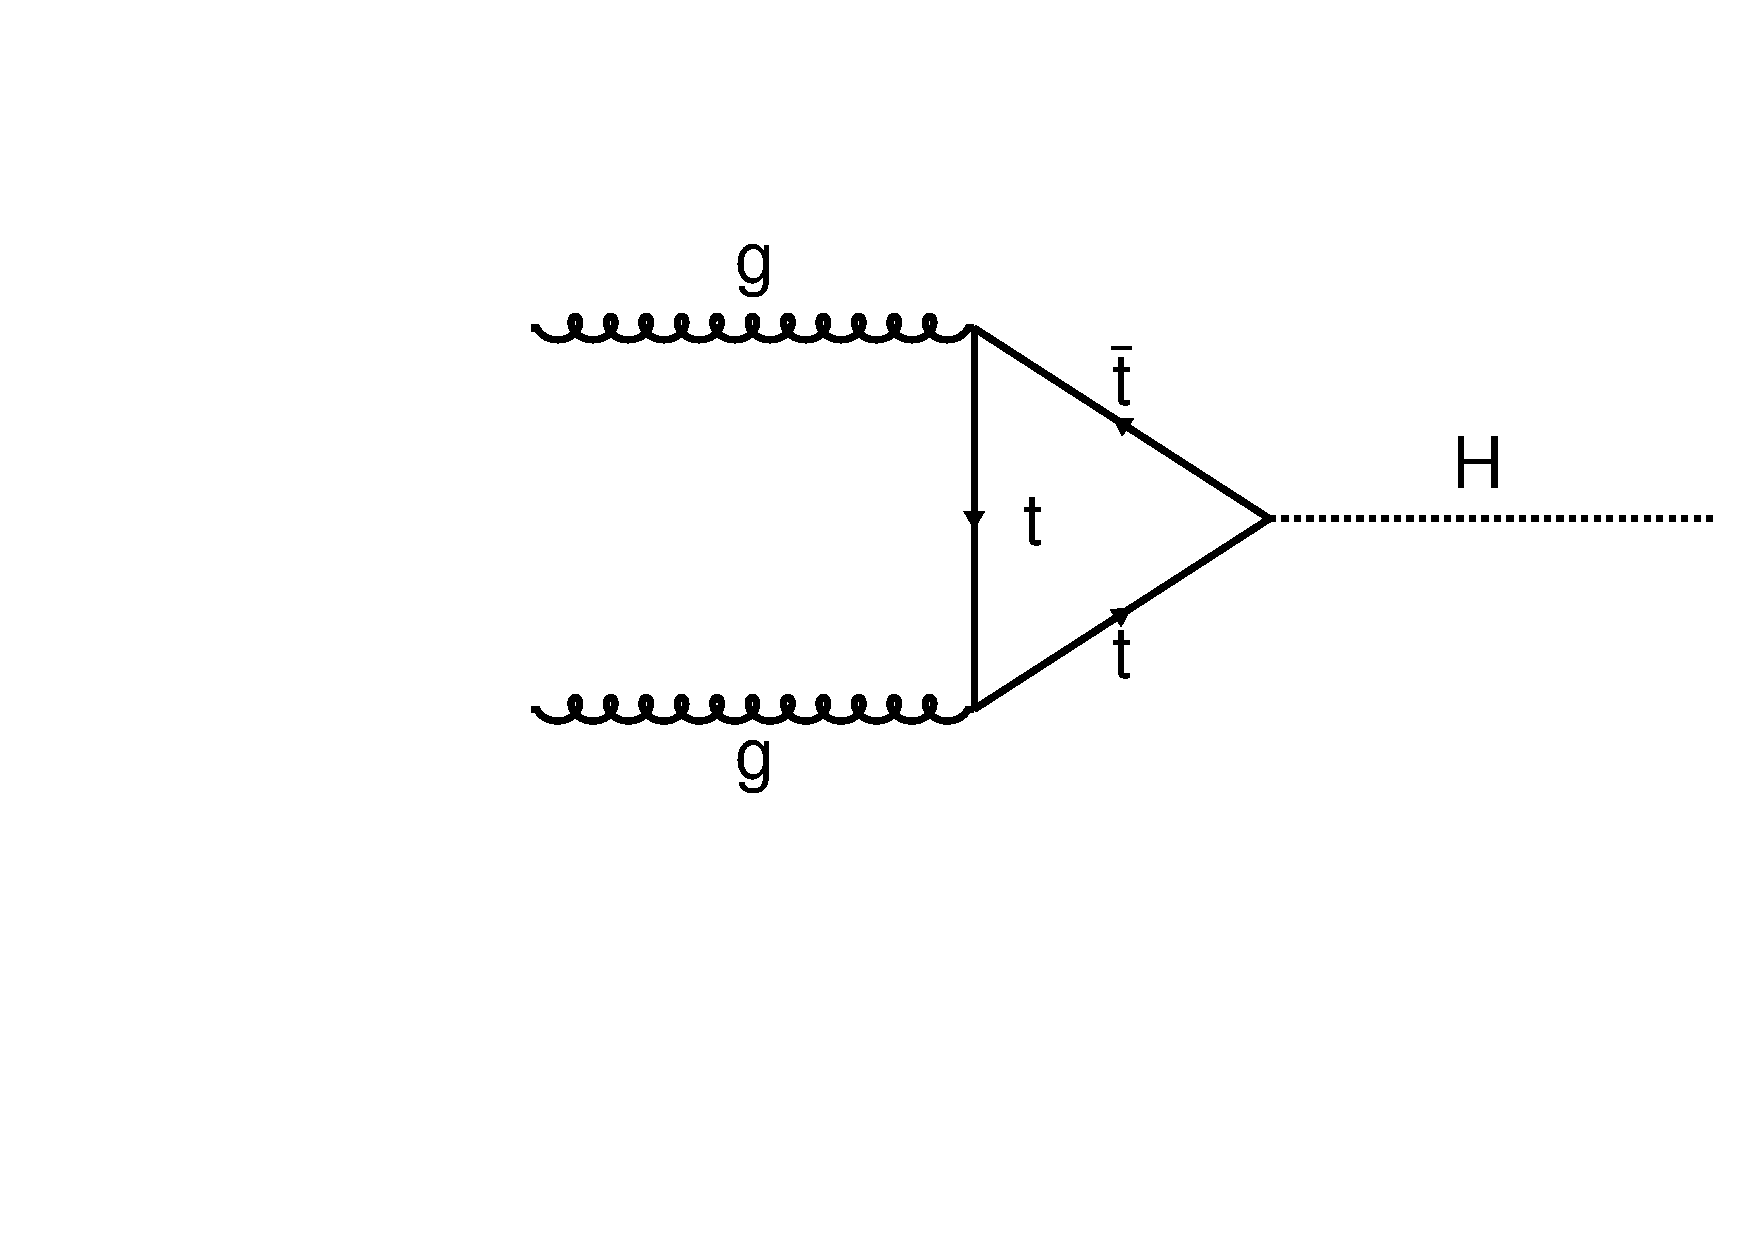
\includegraphics[width=0.45\textwidth]{theory/plots/ggh.pdf}
  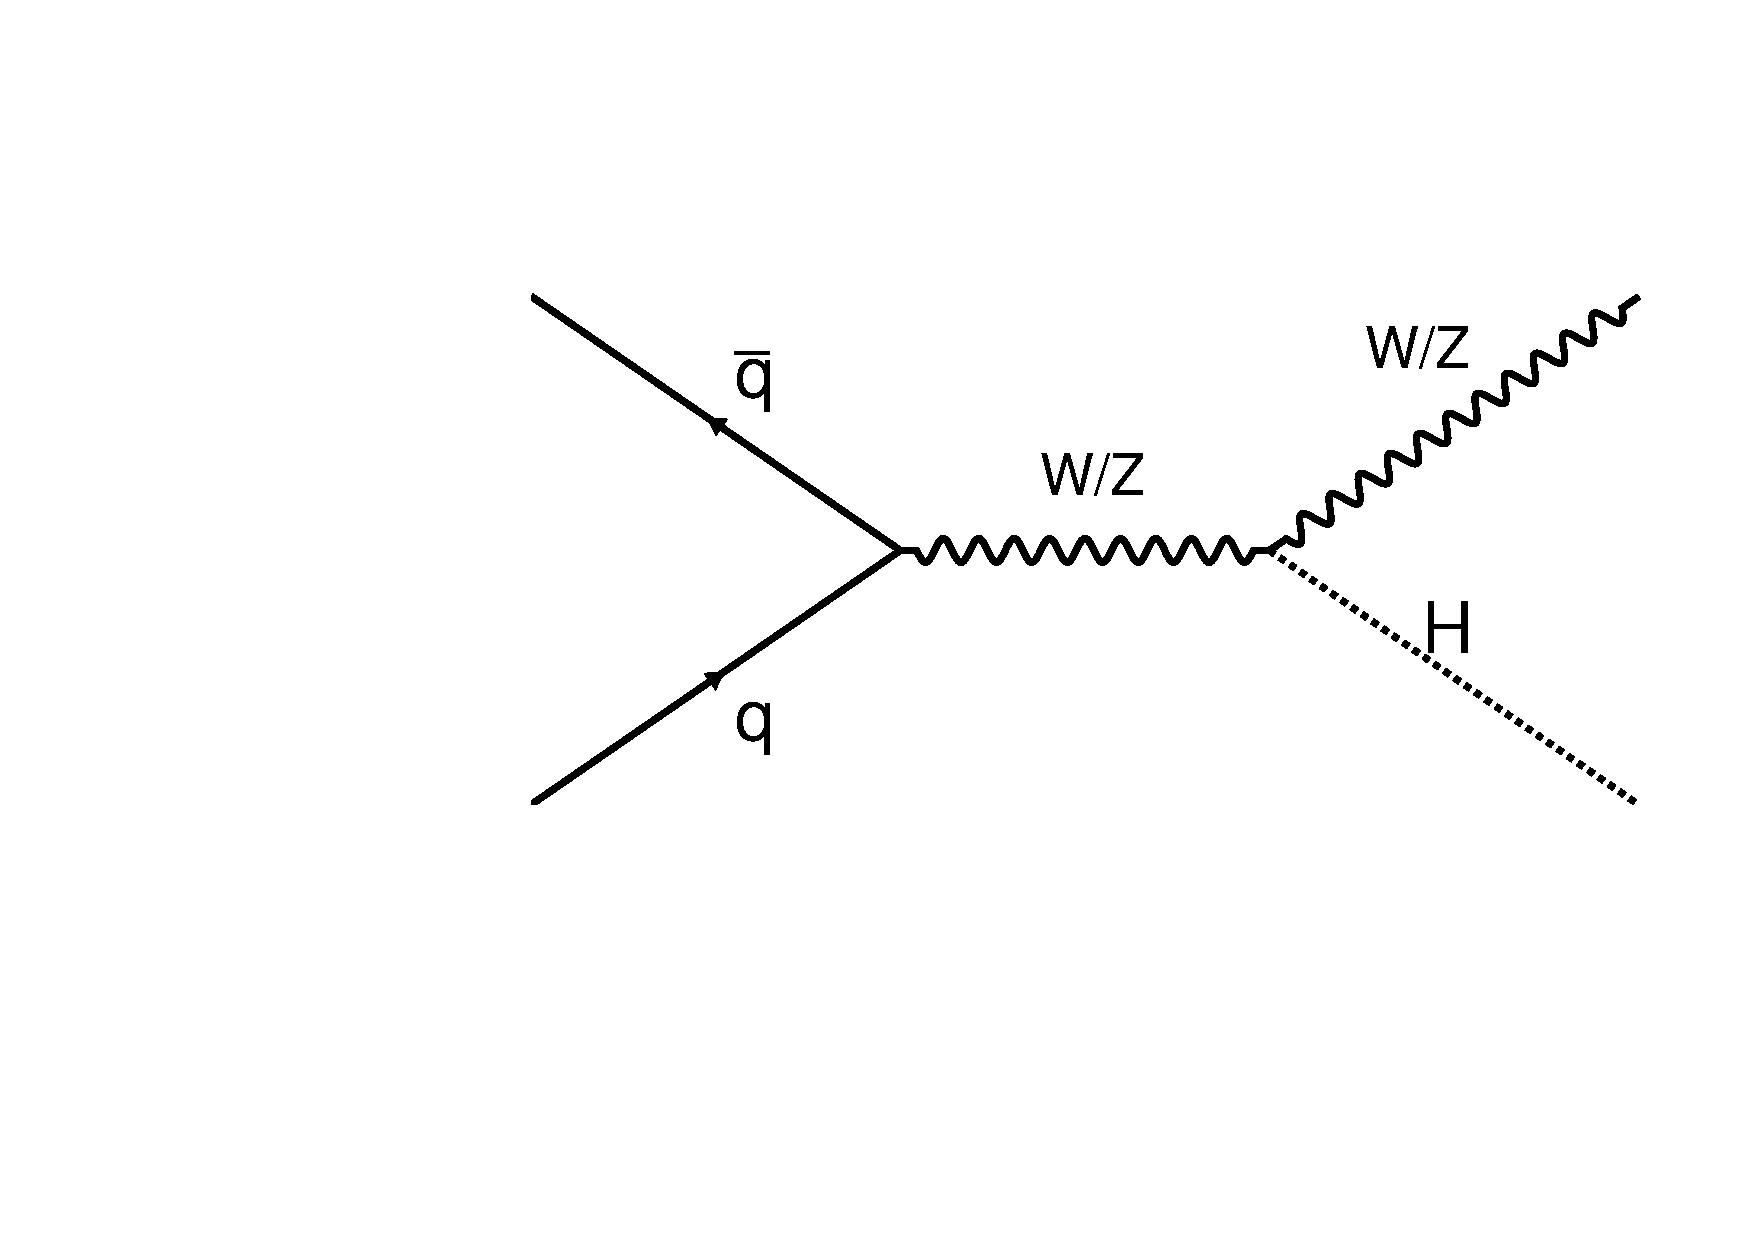
\includegraphics[width=0.45\textwidth]{theory/plots/vh.pdf}\\
  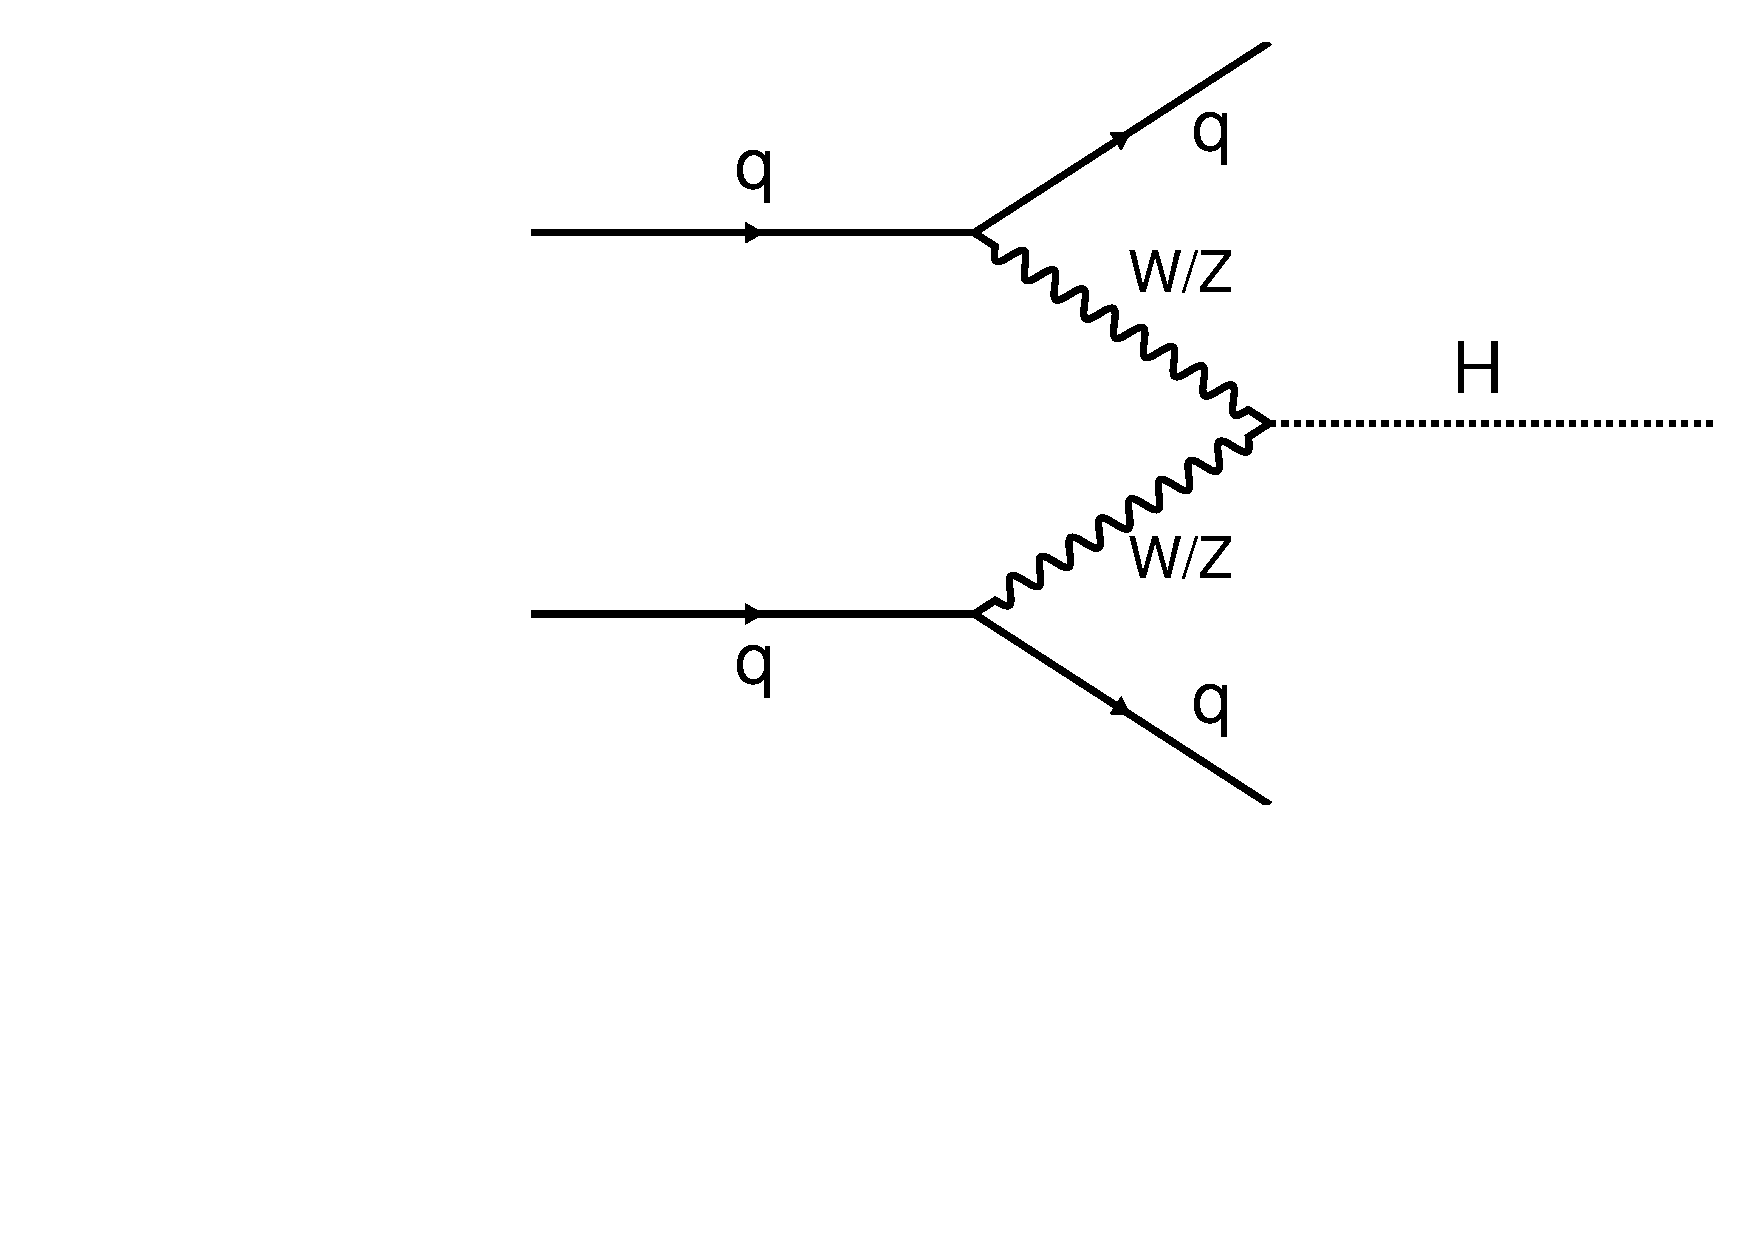
\includegraphics[width=0.45\textwidth]{theory/plots/qqh.pdf}
  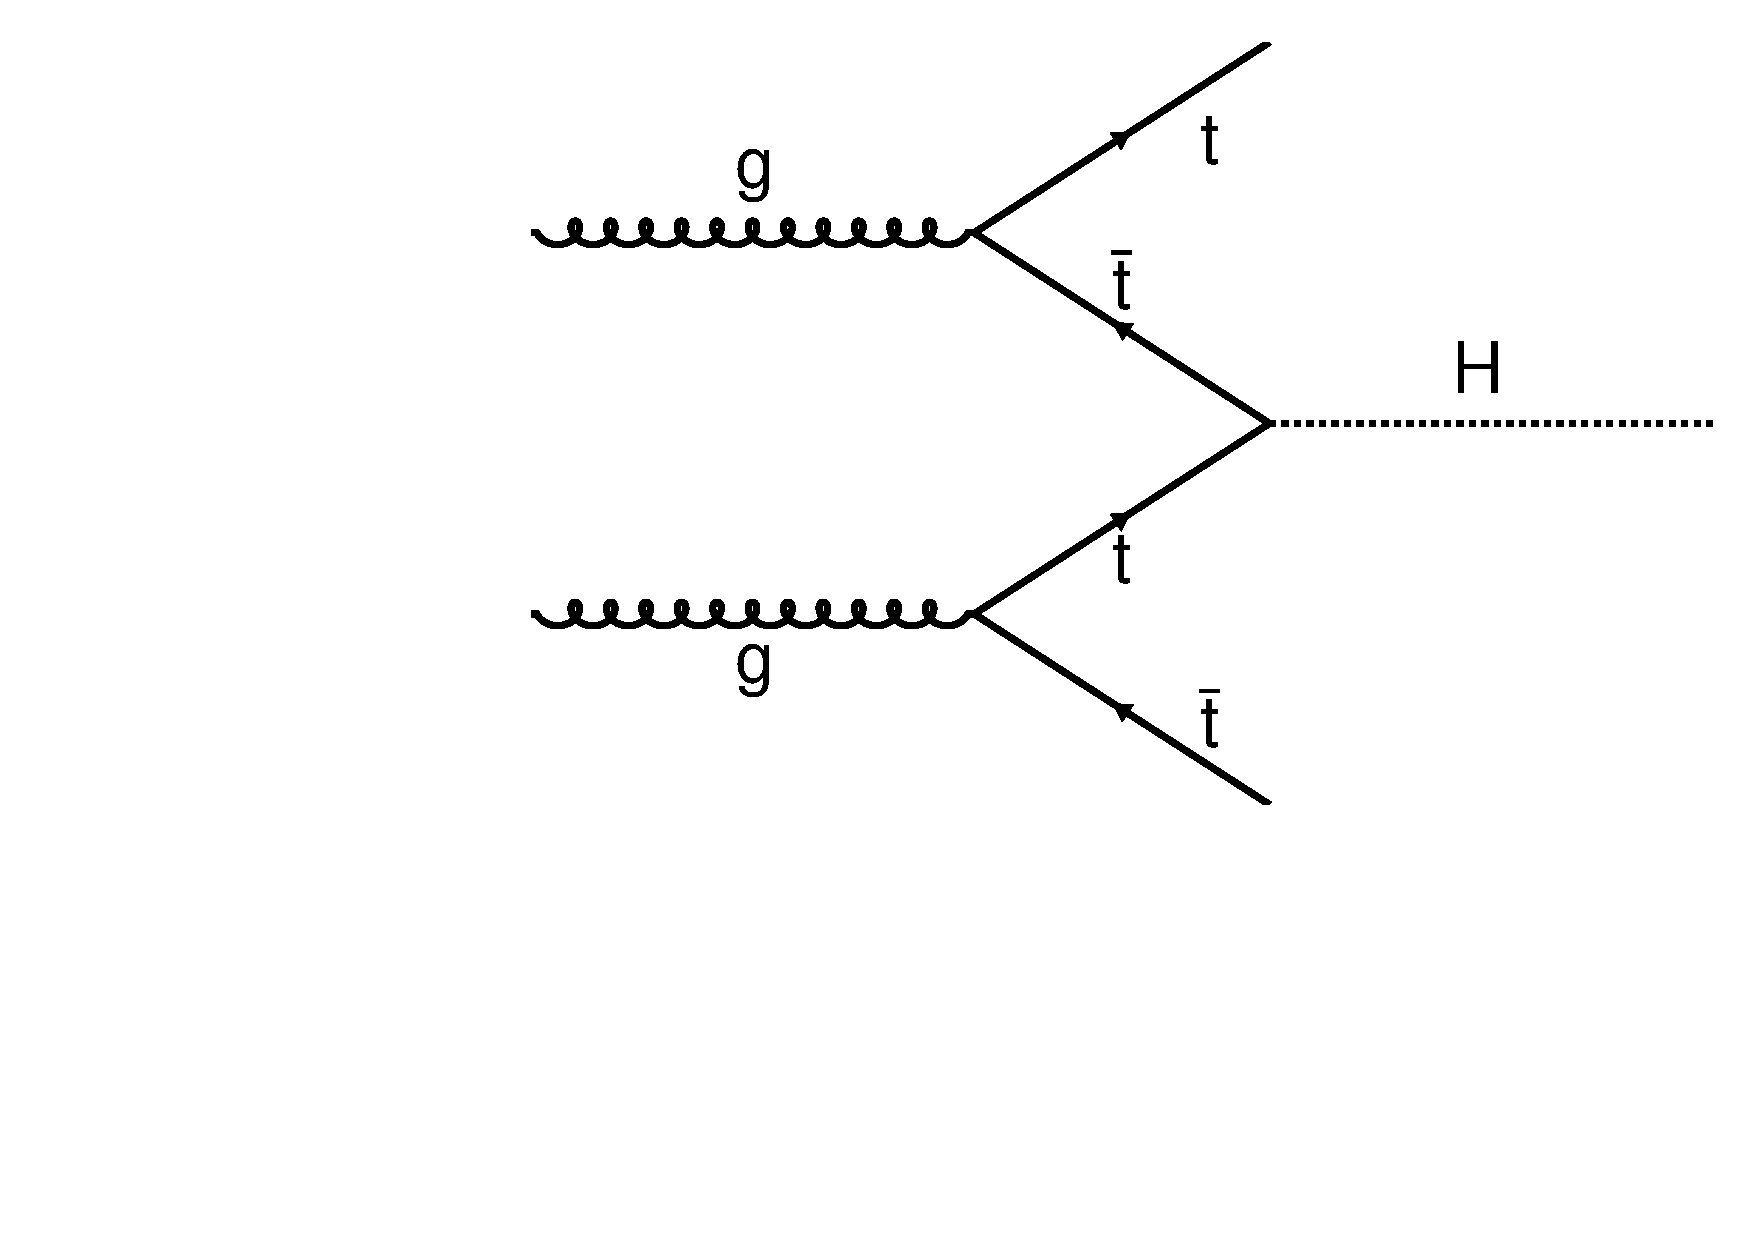
\includegraphics[width=0.45\textwidth]{theory/plots/tth.pdf}
  \caption[Feynman diagrams for \acs{SM} Higgs production at the \acs{LHC}]{The four main \SM Higgs production mechanisms at the LHC: gluon fusion (top left), vector boson fusion (bottom left), $W^{\pm}$ and $Z$ boson associated production (top right) and top anti-top annihilation (bottom right). The cross sections for each of these processes in proton-proton collisions is show in Fig.~\ref{fig:higgs_xs}.}
  \label{fig:feyn_prod}
\end{figure}

A demonstration of the differences between \ggH and \VBF signal is shown in Fig.~\ref{fig:gen_level}. The generator level distributions of these two signals are shown as a function of the generated Higgs transverse momentum and generated Higgs pseudorapidity, \eta, defined as $\eta=-\ln\tan(\theta/2)$, where $\theta$ is the polar angle measured from the beam axis. 
\begin{figure}
  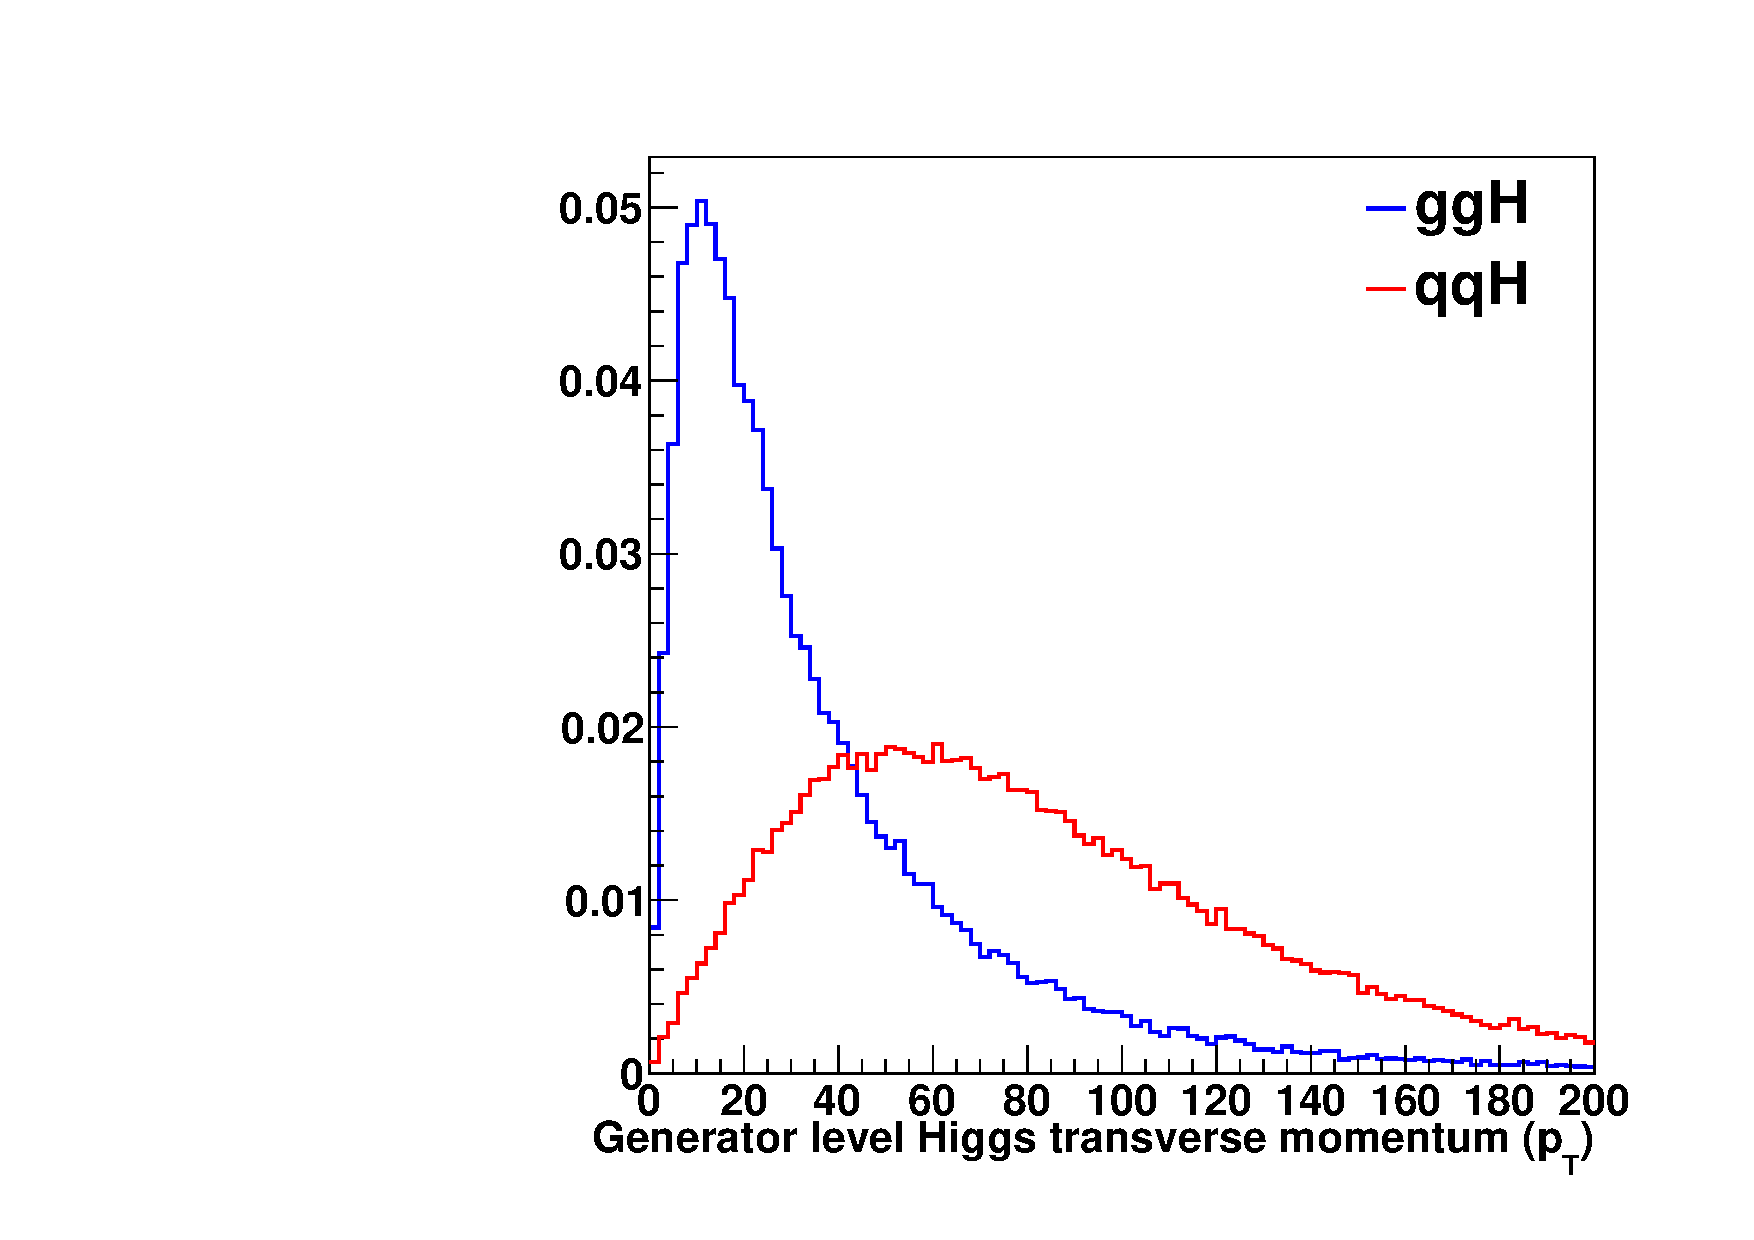
\includegraphics[width=0.45\textwidth]{theory/plots/genPT.pdf}
  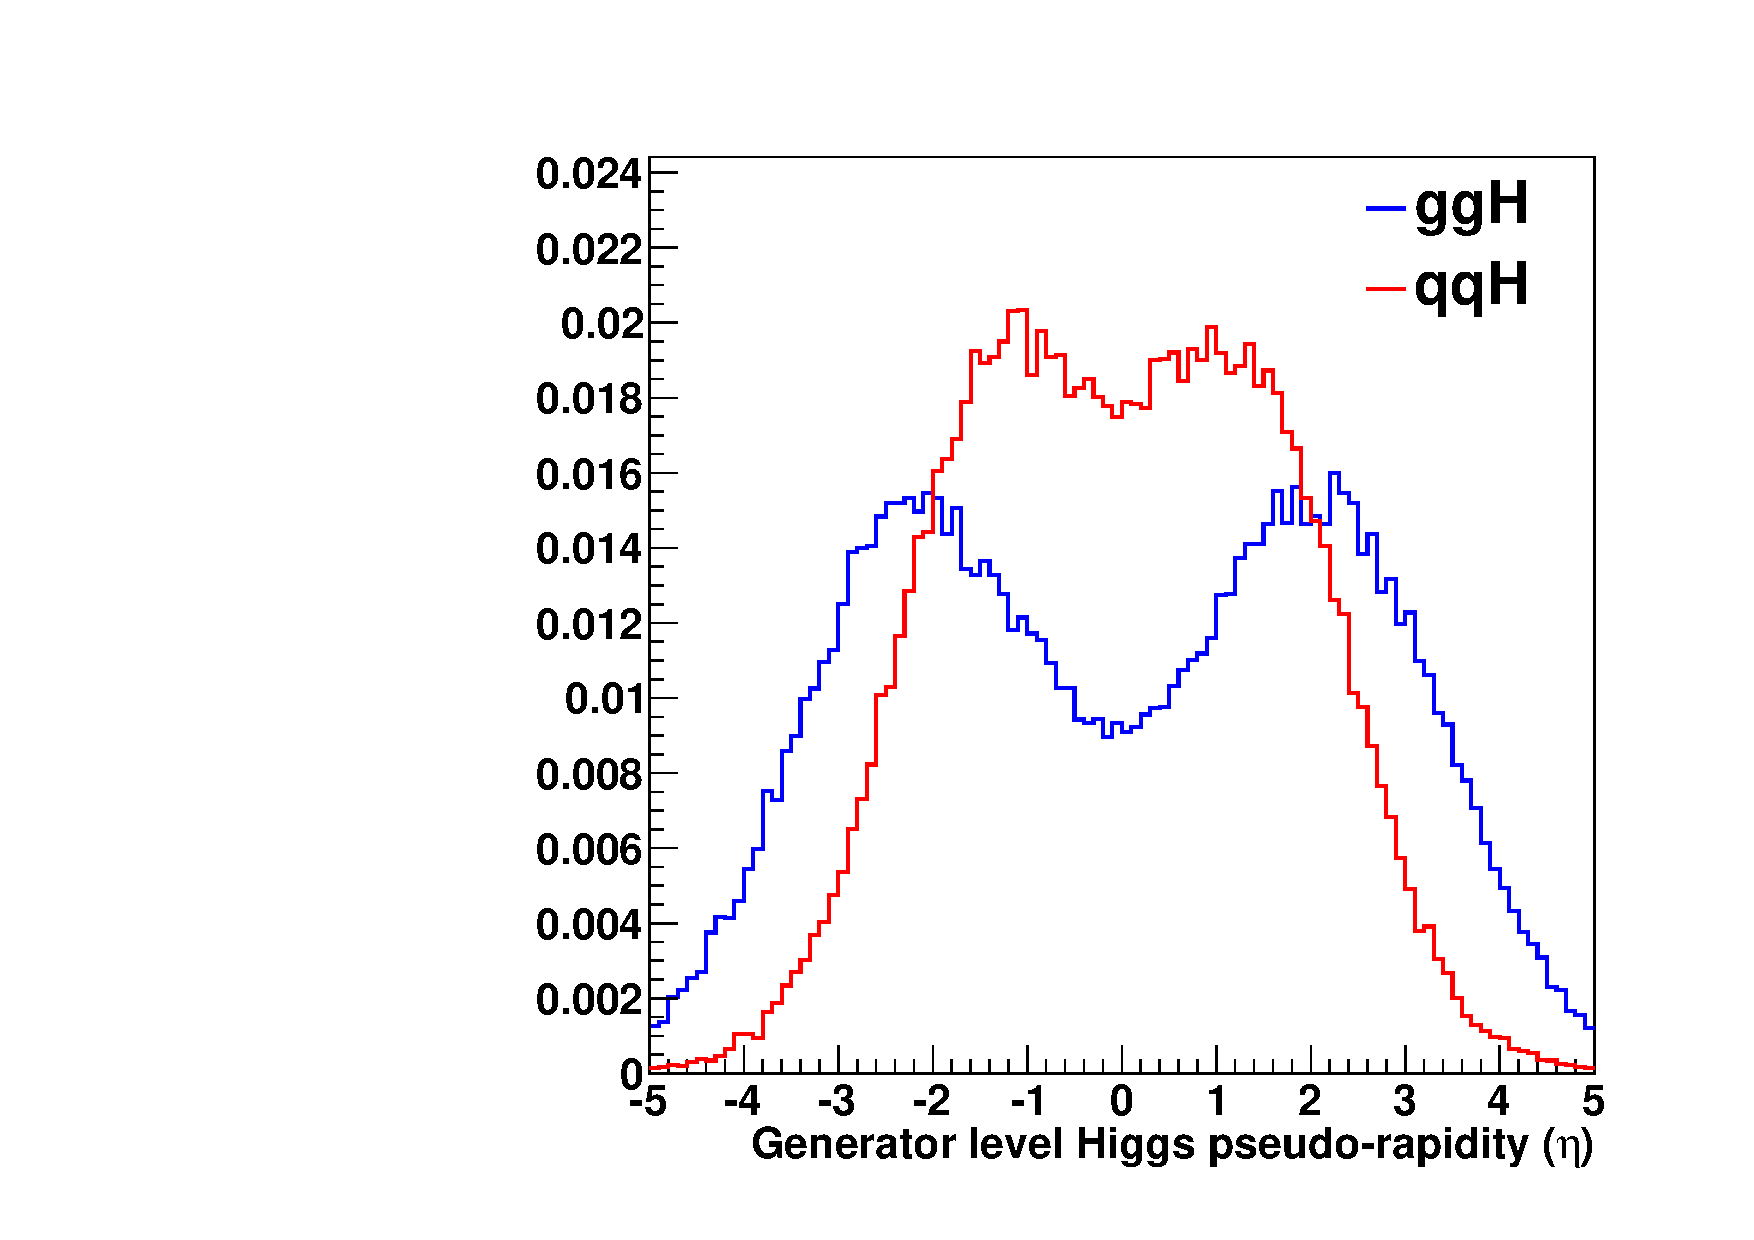
\includegraphics[width=0.45\textwidth]{theory/plots/genEta.pdf}
  \caption[Generator level Higgs distributions]{Generator level Higgs distribution in transverse momentum (left) and pseudorapidity (right) for production via gluon fusion (blue) and vector boson fusion (red).}
  \label{fig:gen_level}
\end{figure}

The \SM Higgs production cross section as a function of the Higgs mass, \mH, is shown for the low mass region $90\leq\mH\leq 300$~\GeV in Fig.~\ref{fig:higgs_xs} for centre-of-mass energies, $\sqrt{s}=7$ and 8~\TeV as provided by the LHC Higgs Cross Section Working Group~\cite{LHCHiggsCrossSectionWorkingGroup3}. It is clear that the production is dominated by \ggH but also that this mechanism has a large theoretical uncertainty. Once the statistics of the \LHC data become very high, this theoretical uncertainty becomes one of the dominant uncertainties in a \Hgg analysis. For a \SM Higgs boson with mass \mH=125~\GeV the cross section is about 18 (22)~pb for $pp$ collisions at $\sqrt{s}=$7 (8)~\TeV.

\begin{figure}
  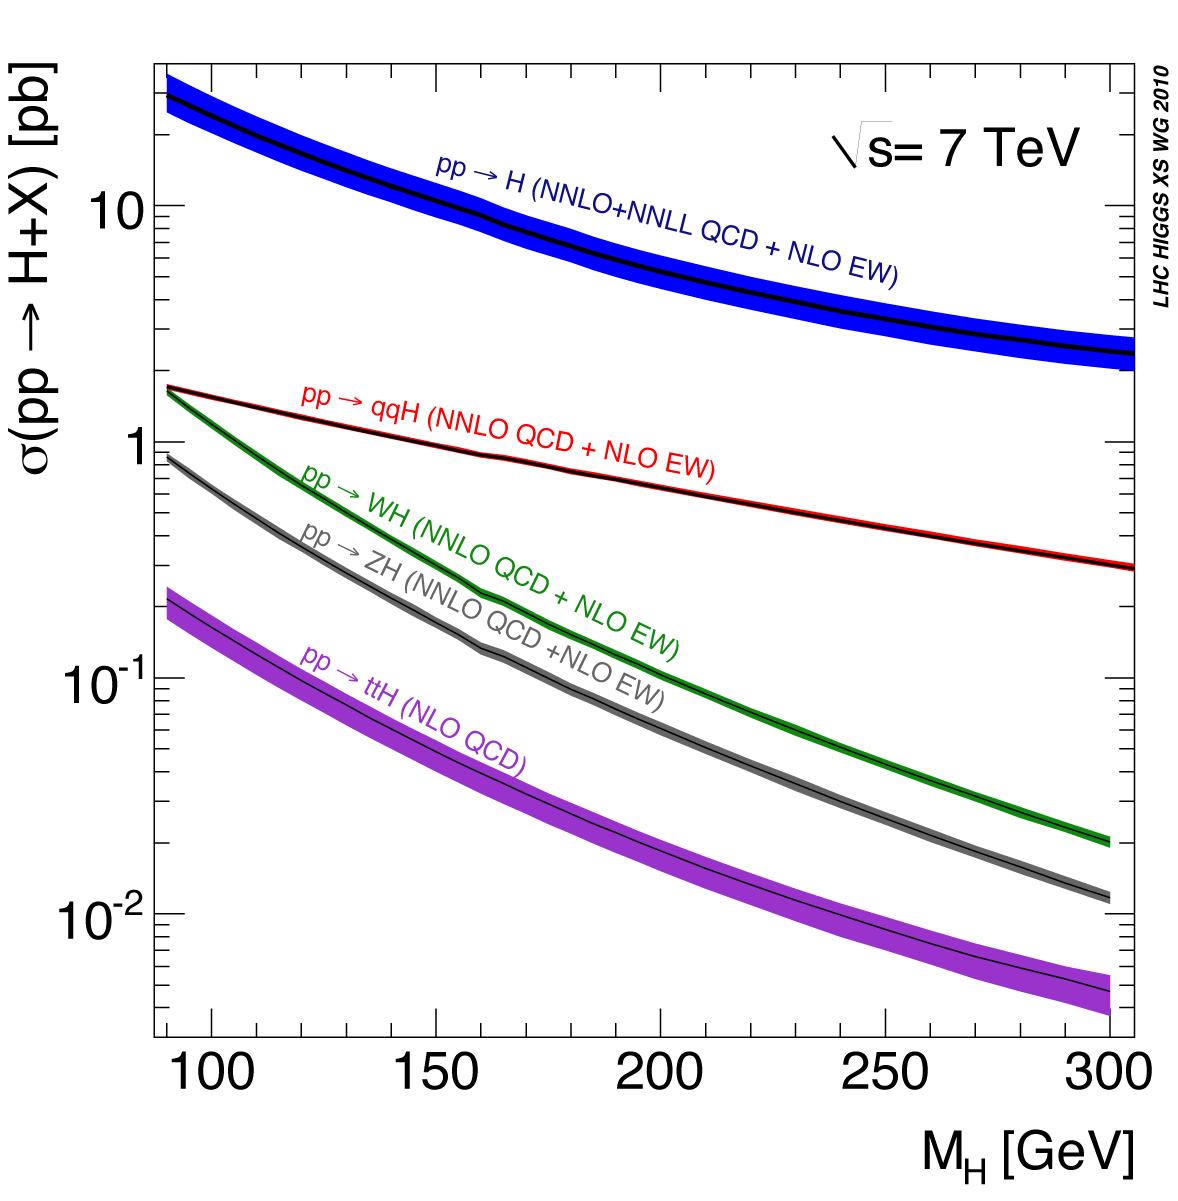
\includegraphics[width=0.48\textwidth]{theory/plots/Higgs_XS_7TeV_LM}
  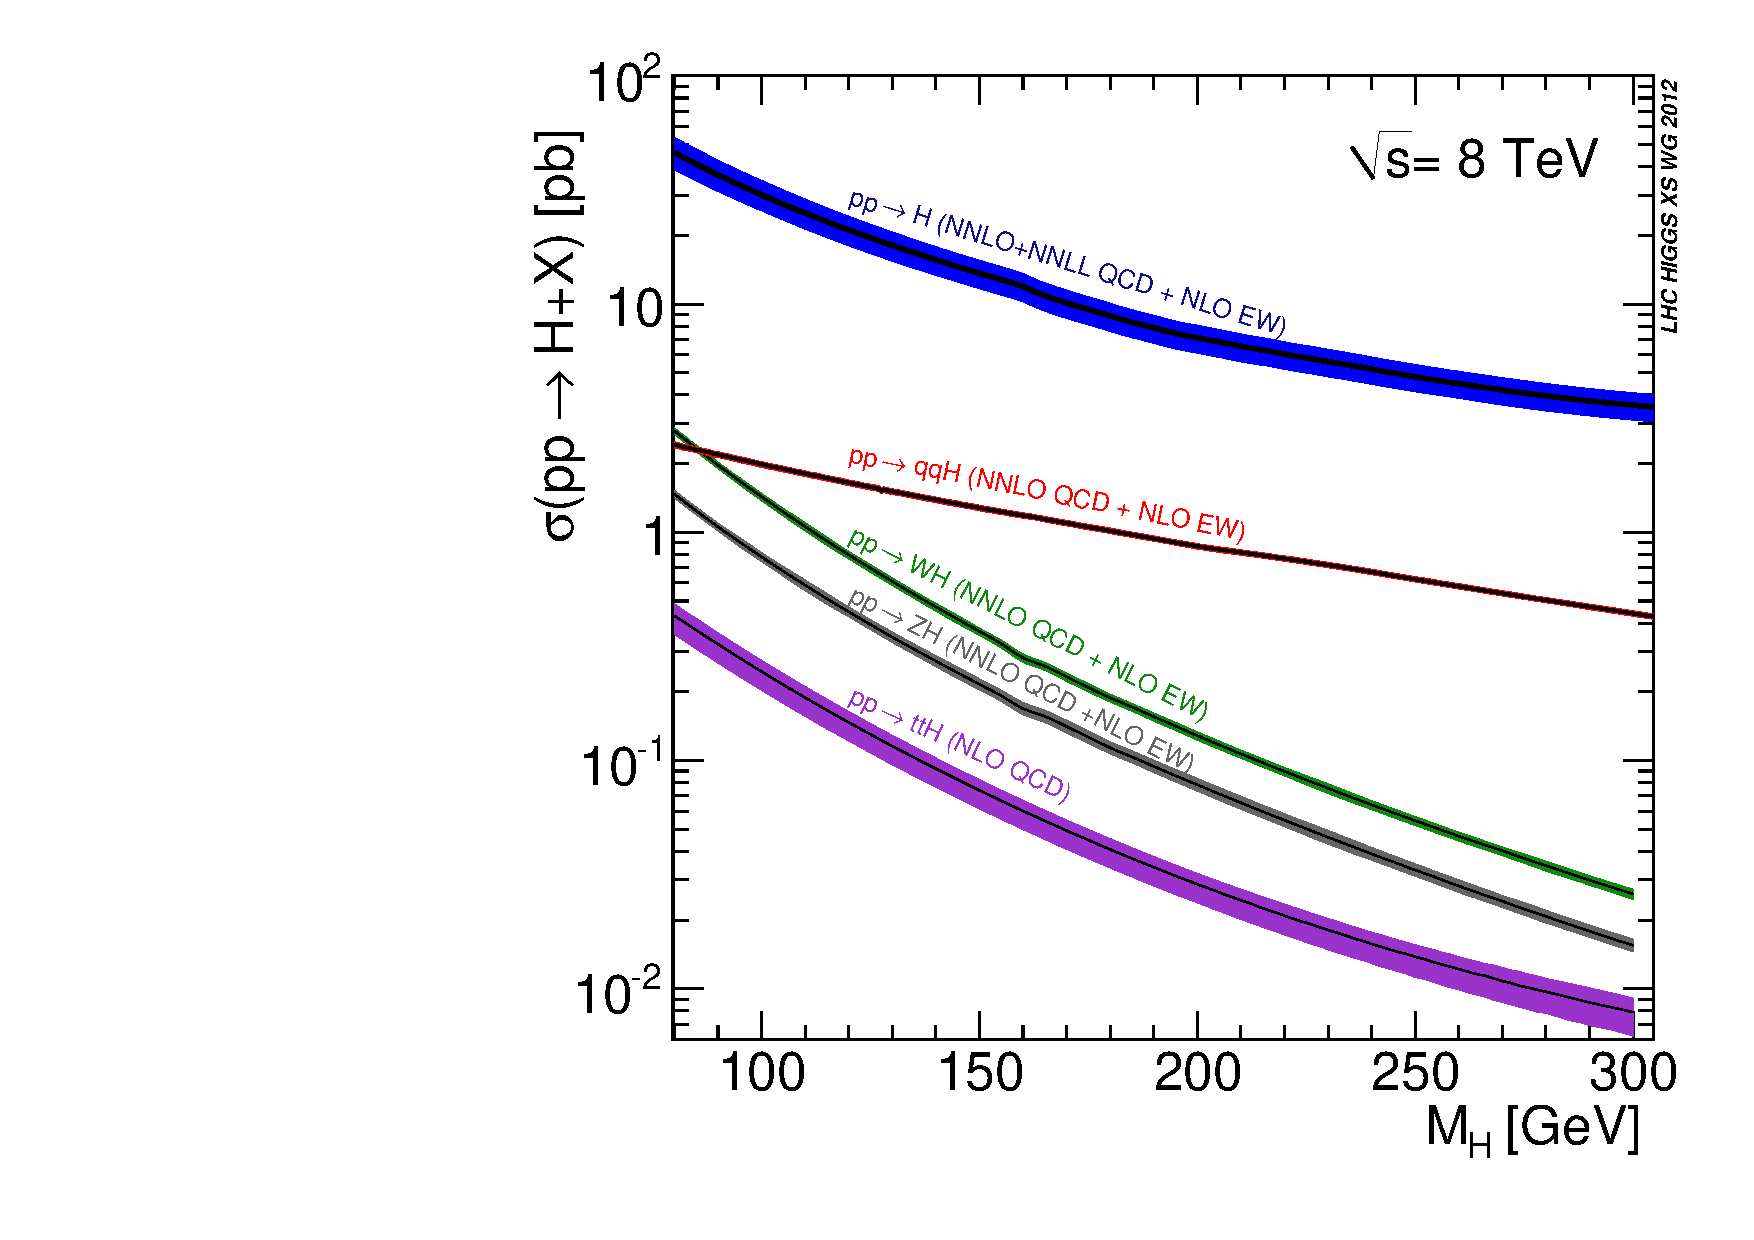
\includegraphics[width=0.48\textwidth]{theory/plots/Higgs_XS_8TeV_LM}
  \caption[\acs{SM} Higgs production cross section at the \acs{LHC}]{The \SM Higgs production cross section in proton-proton collisions at the \LHC for centre-of-mass energies of $\sqrt{s}=7$~\TeV (left) and $\sqrt{s}=8$~\TeV (right). The theoretical uncertainties on the values are shown as the coloured bands. Lines are shown for \ttH production (purple), \ZH production (grey), \WH production (green), \VBF production (red) and \ggH production (blue)~\cite{LHCHiggsCrossSectionWorkingGroup3}.}
  \label{fig:higgs_xs}
\end{figure}

\section{Higgs decay into two photons}

The Higgs couplings are proportional to the mass of the coupling object. Given the photon is massless there is no direct coupling between it and the Higgs. Consequently Higgs decays to photons occur via loop diagrams with $W$ bosons or quarks, of which only the top quark loop need be considered given that the coupling is proportional to the mass and the top quark is considerably heavier than any of the other quarks. The Feynman diagrams for these processes at leading order are shown in Fig.~\ref{fig:feyn_hgg_decay}.

\begin{figure}
  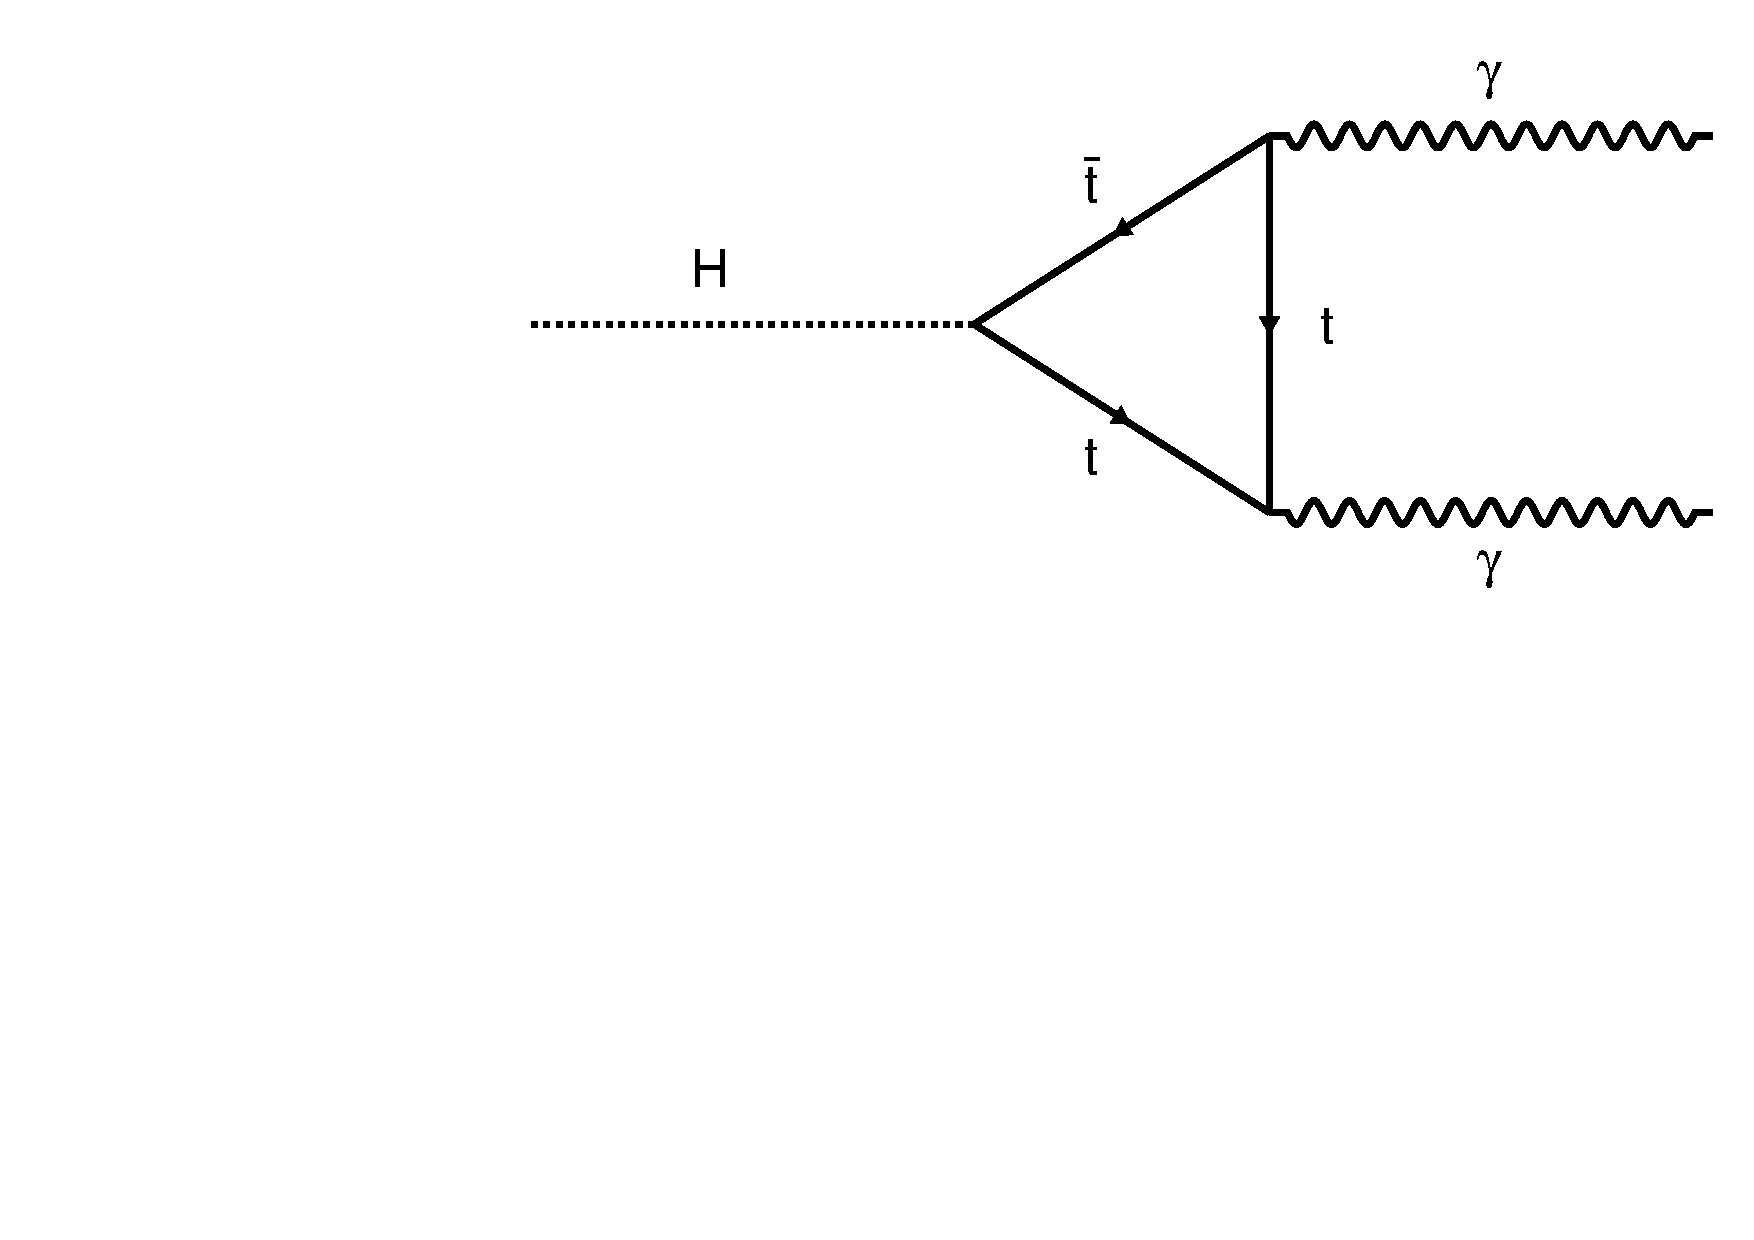
\includegraphics[width=0.32\textwidth]{theory/plots/Htgg.pdf}
  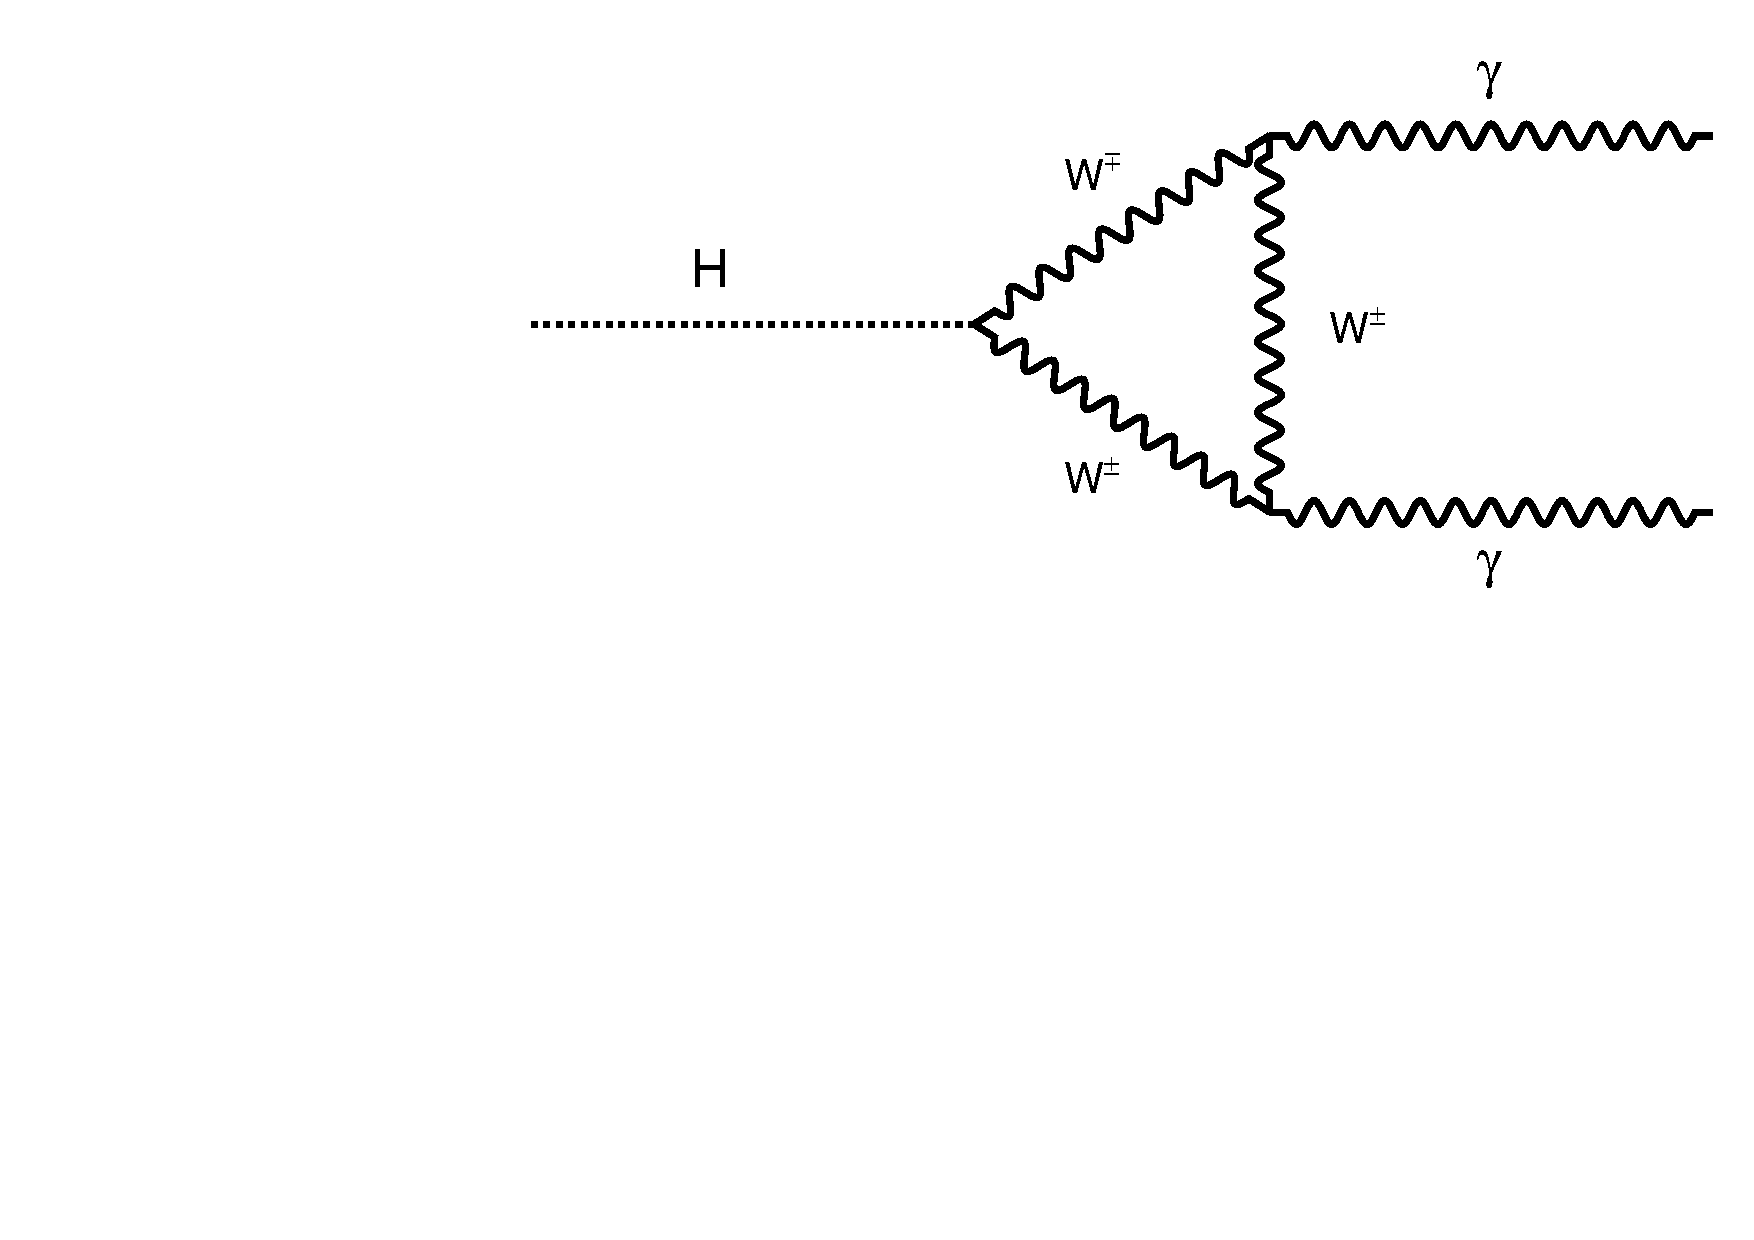
\includegraphics[width=0.32\textwidth]{theory/plots/HWgg.pdf}
  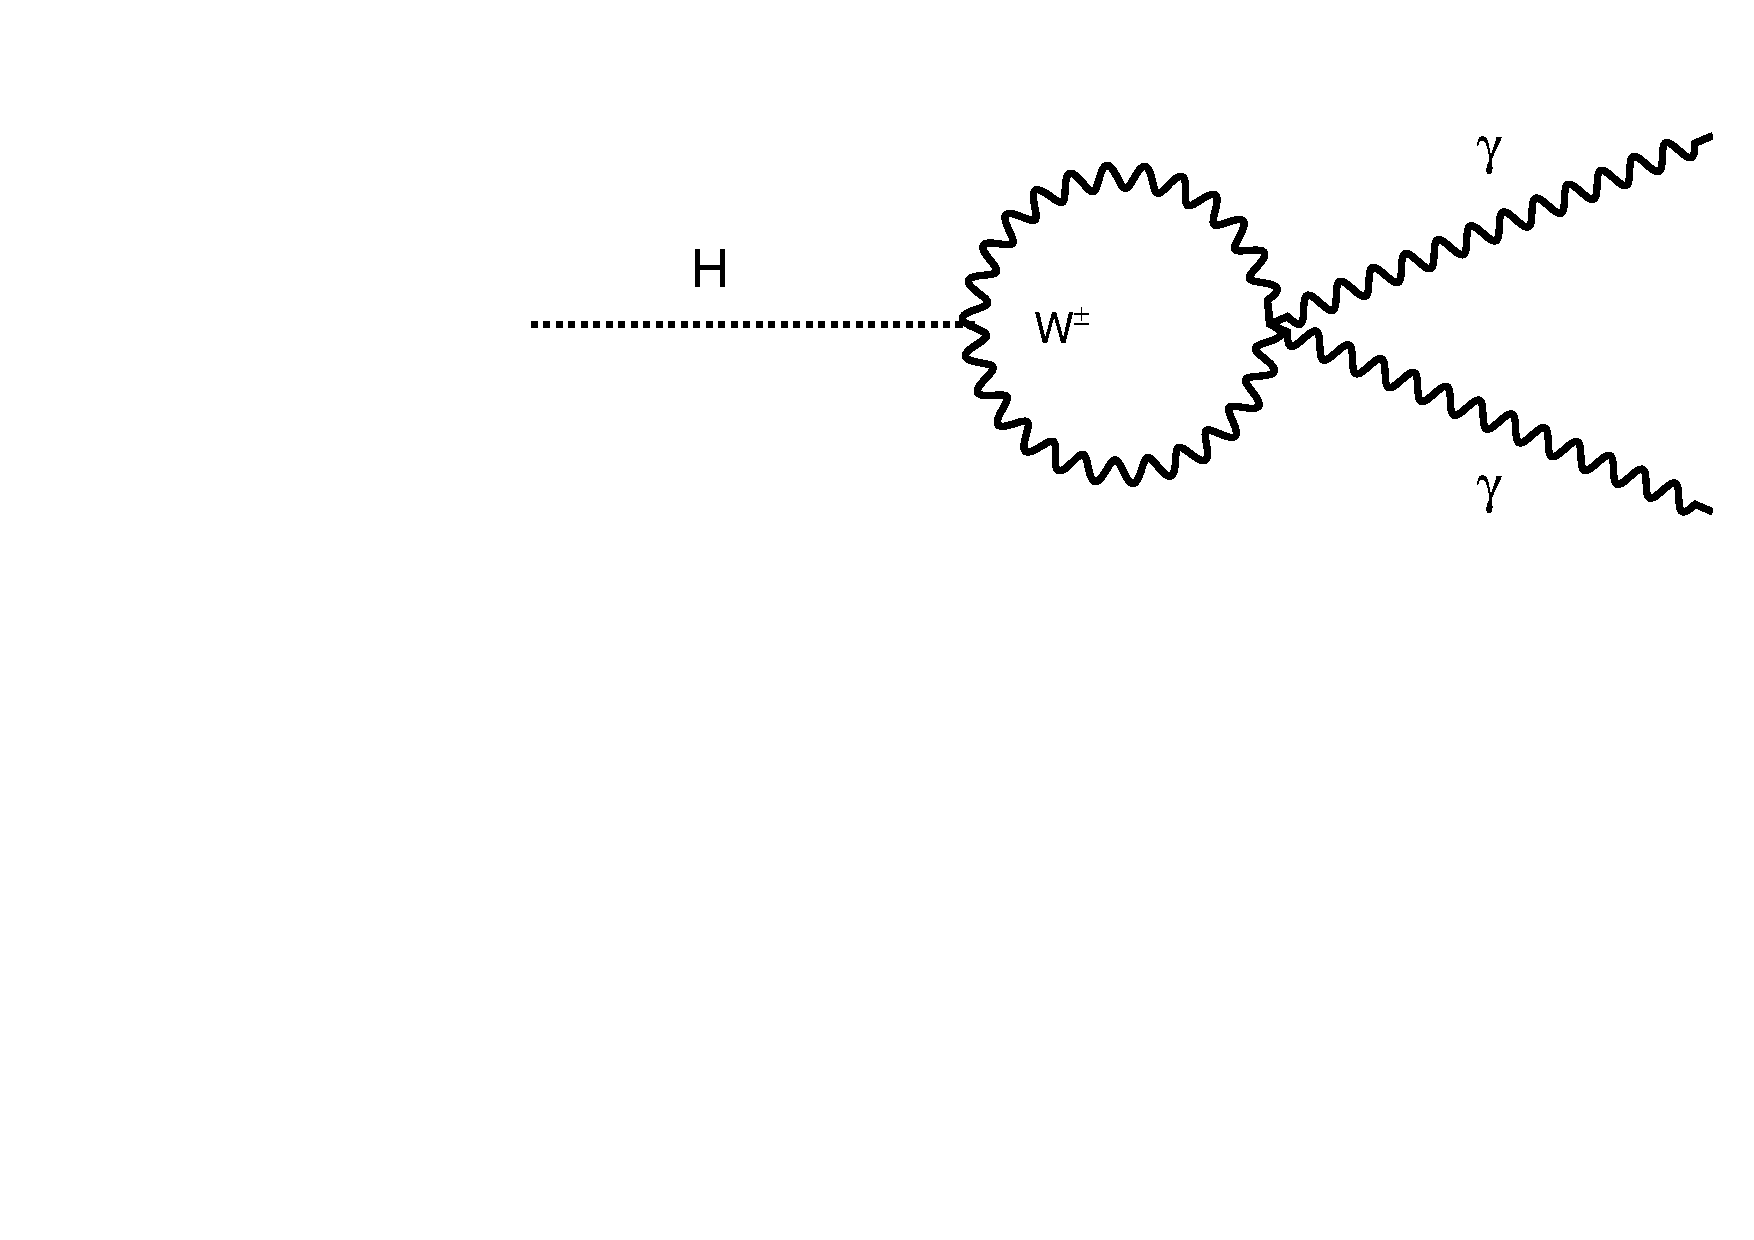
\includegraphics[width=0.32\textwidth]{theory/plots/HWgg4.pdf}
  \caption{Feynman diagrams for the \acs{SM} Higgs to two photon decay at leading order.}
  \label{fig:feyn_hgg_decay}
\end{figure}


The \SM Higgs branching ratio for each set of decay products is shown as a function of the Higgs mass, \mH, for the low mass region $80\leq\mH\leq 200$~\GeV in Fig.~\ref{fig:higgs_br} as provided by the LHC Higgs Cross Section Working Group~\cite{LHCHiggsCrossSectionWorkingGroup3}. The work in this thesis focuses on the Higgs decay into two photons (\Hgg) whose branching fraction is shown by the pink line. It is apparent that \Hgg decays are rare. There is only a small window of Higgs masses in which \Hgg decay is even feasible (\mH$<\sim185$~\GeV) and the peak of the branching fraction ($120<\mH<130$~\GeV) only allows a \SM \Hgg decay 0.2\% of the time. Given that the \LHC Run 1 dataset used in this thesis consists of 5.1\fbinv at \sqrts=7~\TeV and 19.7\fbinv at \sqrts=8~\TeV one can expect about 1/2 million \SM Higgs boson to be produced (assuming a value of \mH=125~\GeV) of which only about 1000 decay into two photons. 

\begin{figure}
  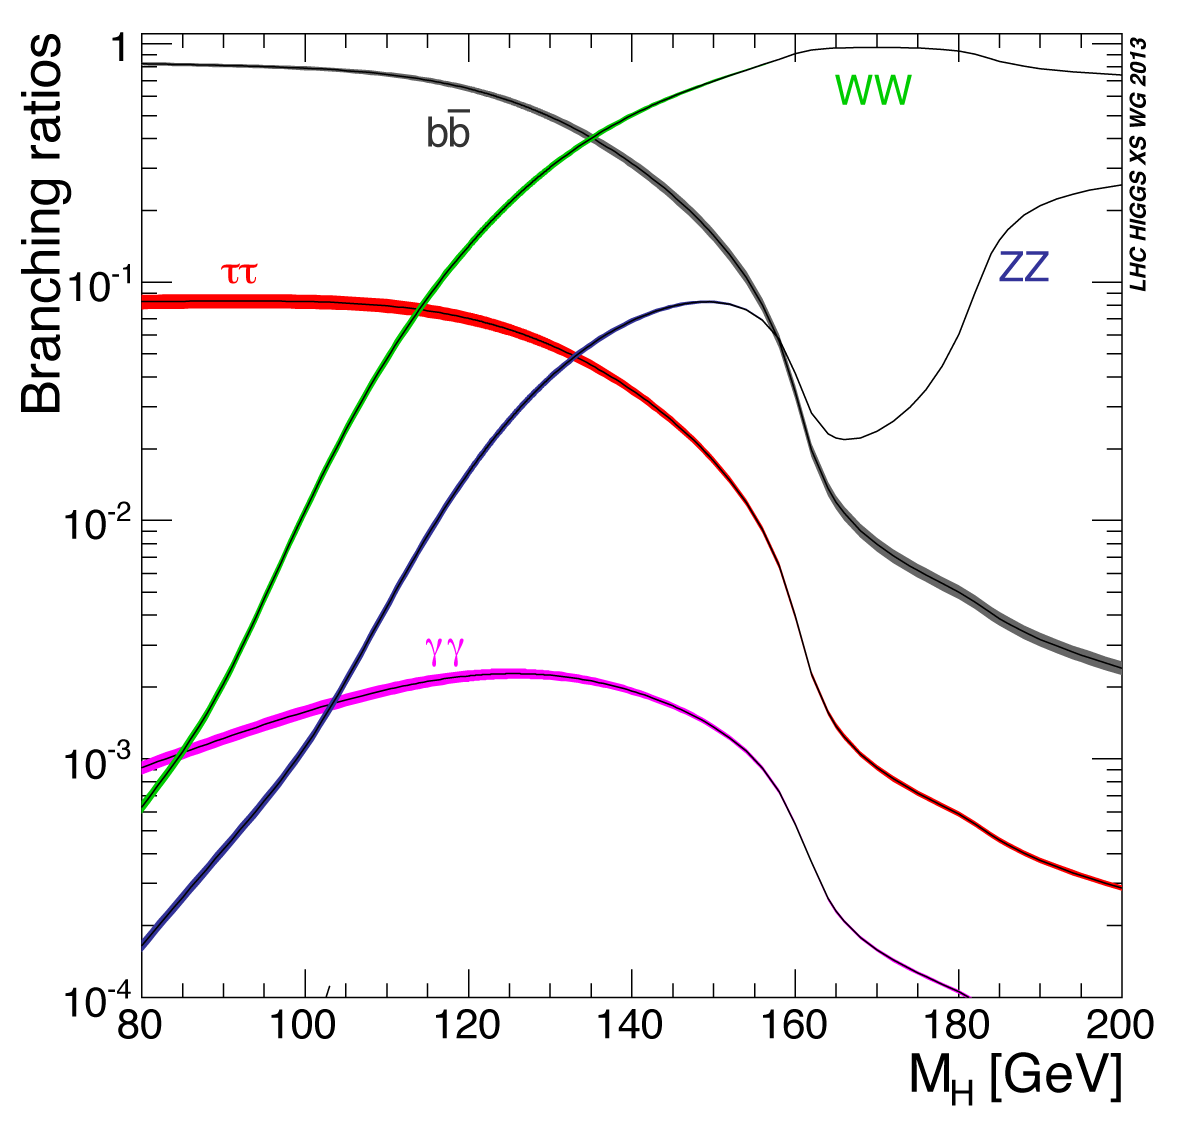
\includegraphics[width=0.6\textwidth]{theory/plots/Higgs_BR_LM}
  \caption[\acs{SM} Higgs branching fraction]{A plot showing the branching ratio of the \SM Higgs boson into various decay products as a function of the Higgs mass \mH. The theoretical uncertainties are shown as the coloured bands. Only the primary search channels are left on this figure (Higgs decaying into $b\bar{b}$, $ZZ$, $WW$, $\tau\tau$ and $\gamma\gamma$) for ease of viewing, there are several other possibilities left out (Higgs decaying into $gg$, $c\bar{c}$, $Z\gamma$, $\mu\mu$). This thesis concentrates on the \Hgg decay shown as the pink line~\cite{LHCHiggsCrossSectionWorkingGroup3}.}
  \label{fig:higgs_br}
\end{figure}

\subsection{Backgrounds to the \Hgg decay at the \LHC}

Aside from the very low signal rate of Higgs decays to two photons, further complications arise by considering the incredibly high rate of the background processes for two photon production in proton-proton collisions. A pair of real (prompt) photons is predominantly produced by \QCD interactions from a proton-proton initial state via two diagrams; the so called Born ($q\bar{q}\rightarrow\gamma\gamma$) and the box ($gg\rightarrow\gamma\gamma$), collectively known as \textit{prompt-prompt} background. These two backgrounds are referred to as irreducuble as they fake signal with two real photons. By using the specific kinematics of Higgs decays these backgrounds can be somewhat suppressed but the main challenge of the analysis is estimating the contamination of these processes in the signal region. The other type of background arises from final state neutral hadrons faking photons. Predominantly these are $\pi^{0}$s decaying into two almost collinear photons which fake the single photon signal. This can happen in association with one real photon, \gjet (known as \textit{prompt-fake}), or where both photons are faked by jet signals (known as \textit{fake-fake}). Nearly all of the \textit{fake-fake} background can be removed using the analysis techniques described in Chapters~\ref{chap:common_analysis_components} and~\ref{chap:selection_and_categorisation} such that the final analysis consists of about 70\% prompt-prompt, 30\% prompt-fake and $<1\%$ fake-fake. The Feynman diagrams for Born, box and \gjet production are shown in Fig.~\ref{fig:feyn_bkgs}.

\begin{figure}
  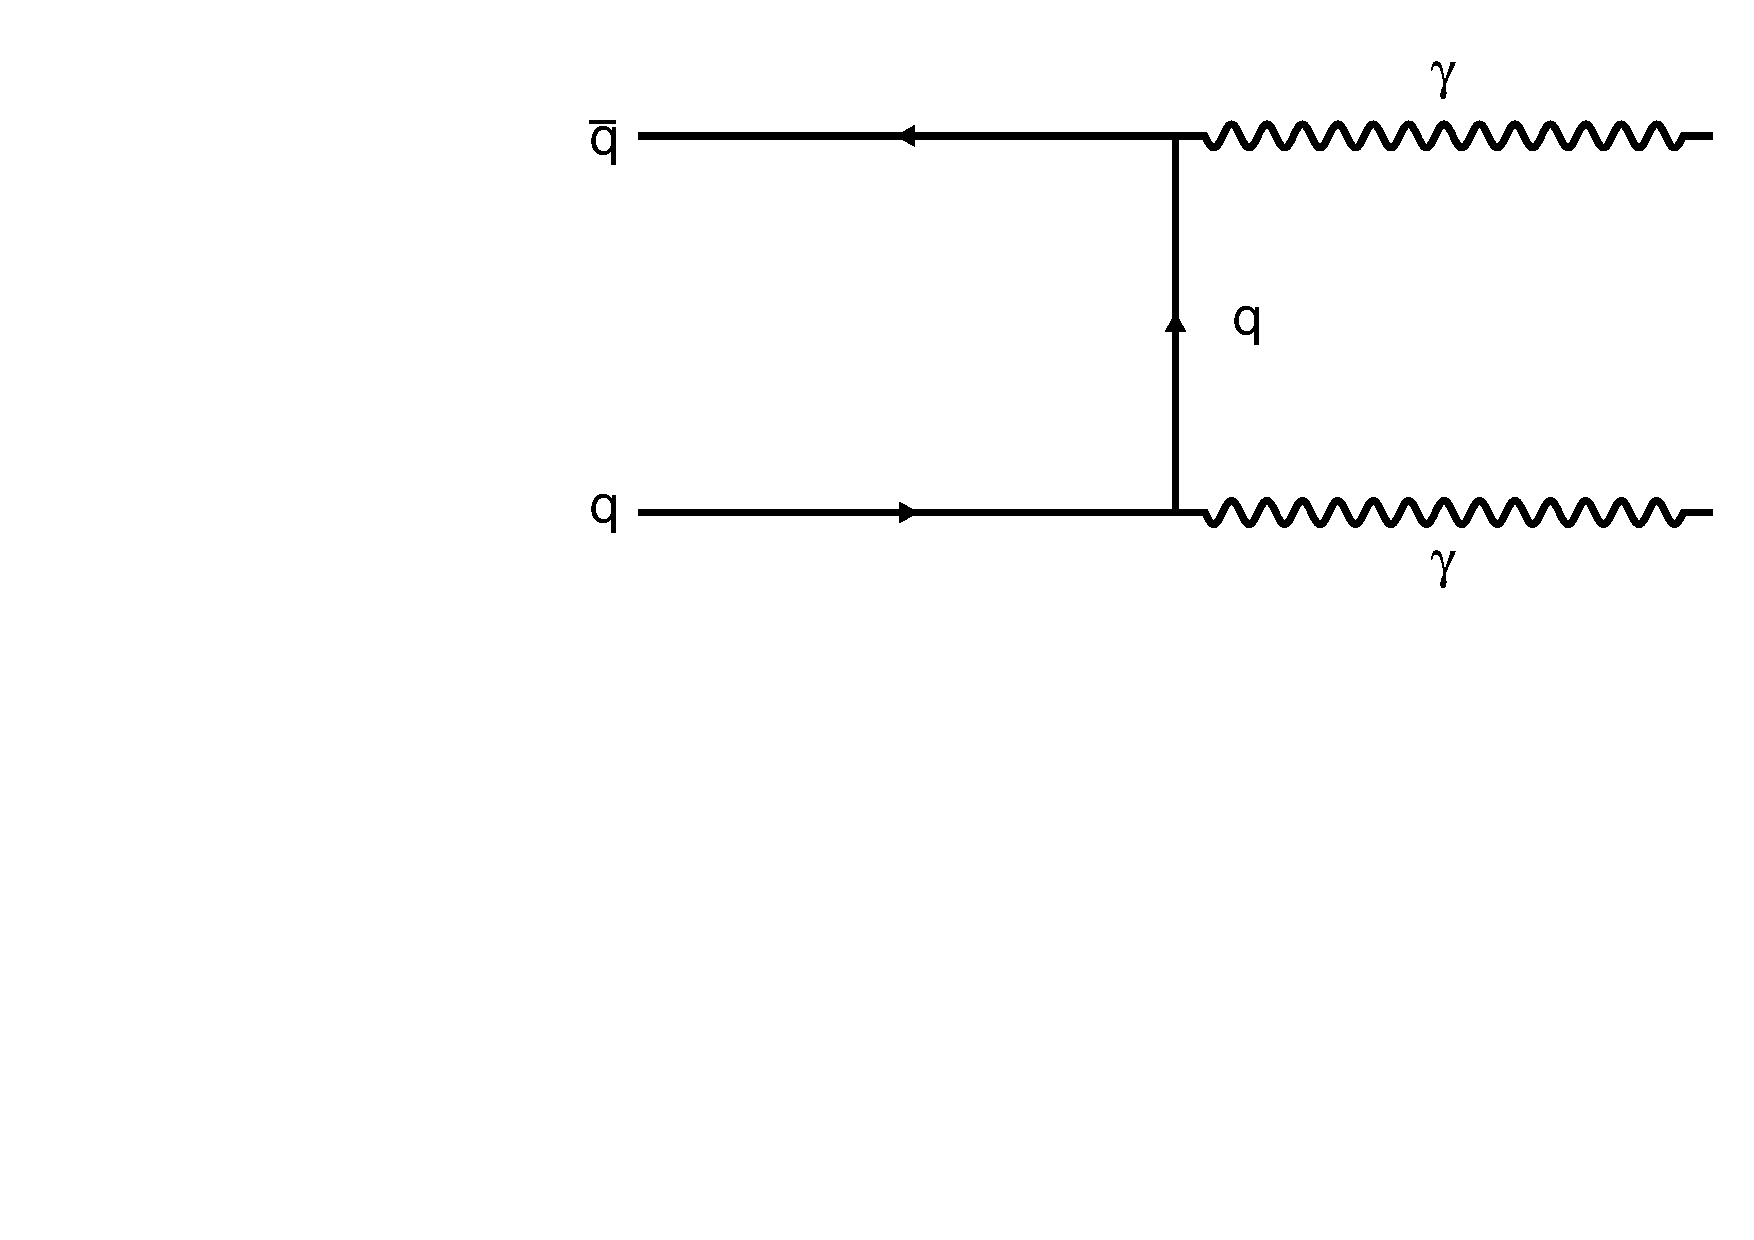
\includegraphics[width=0.32\textwidth]{theory/plots/Born.pdf}
  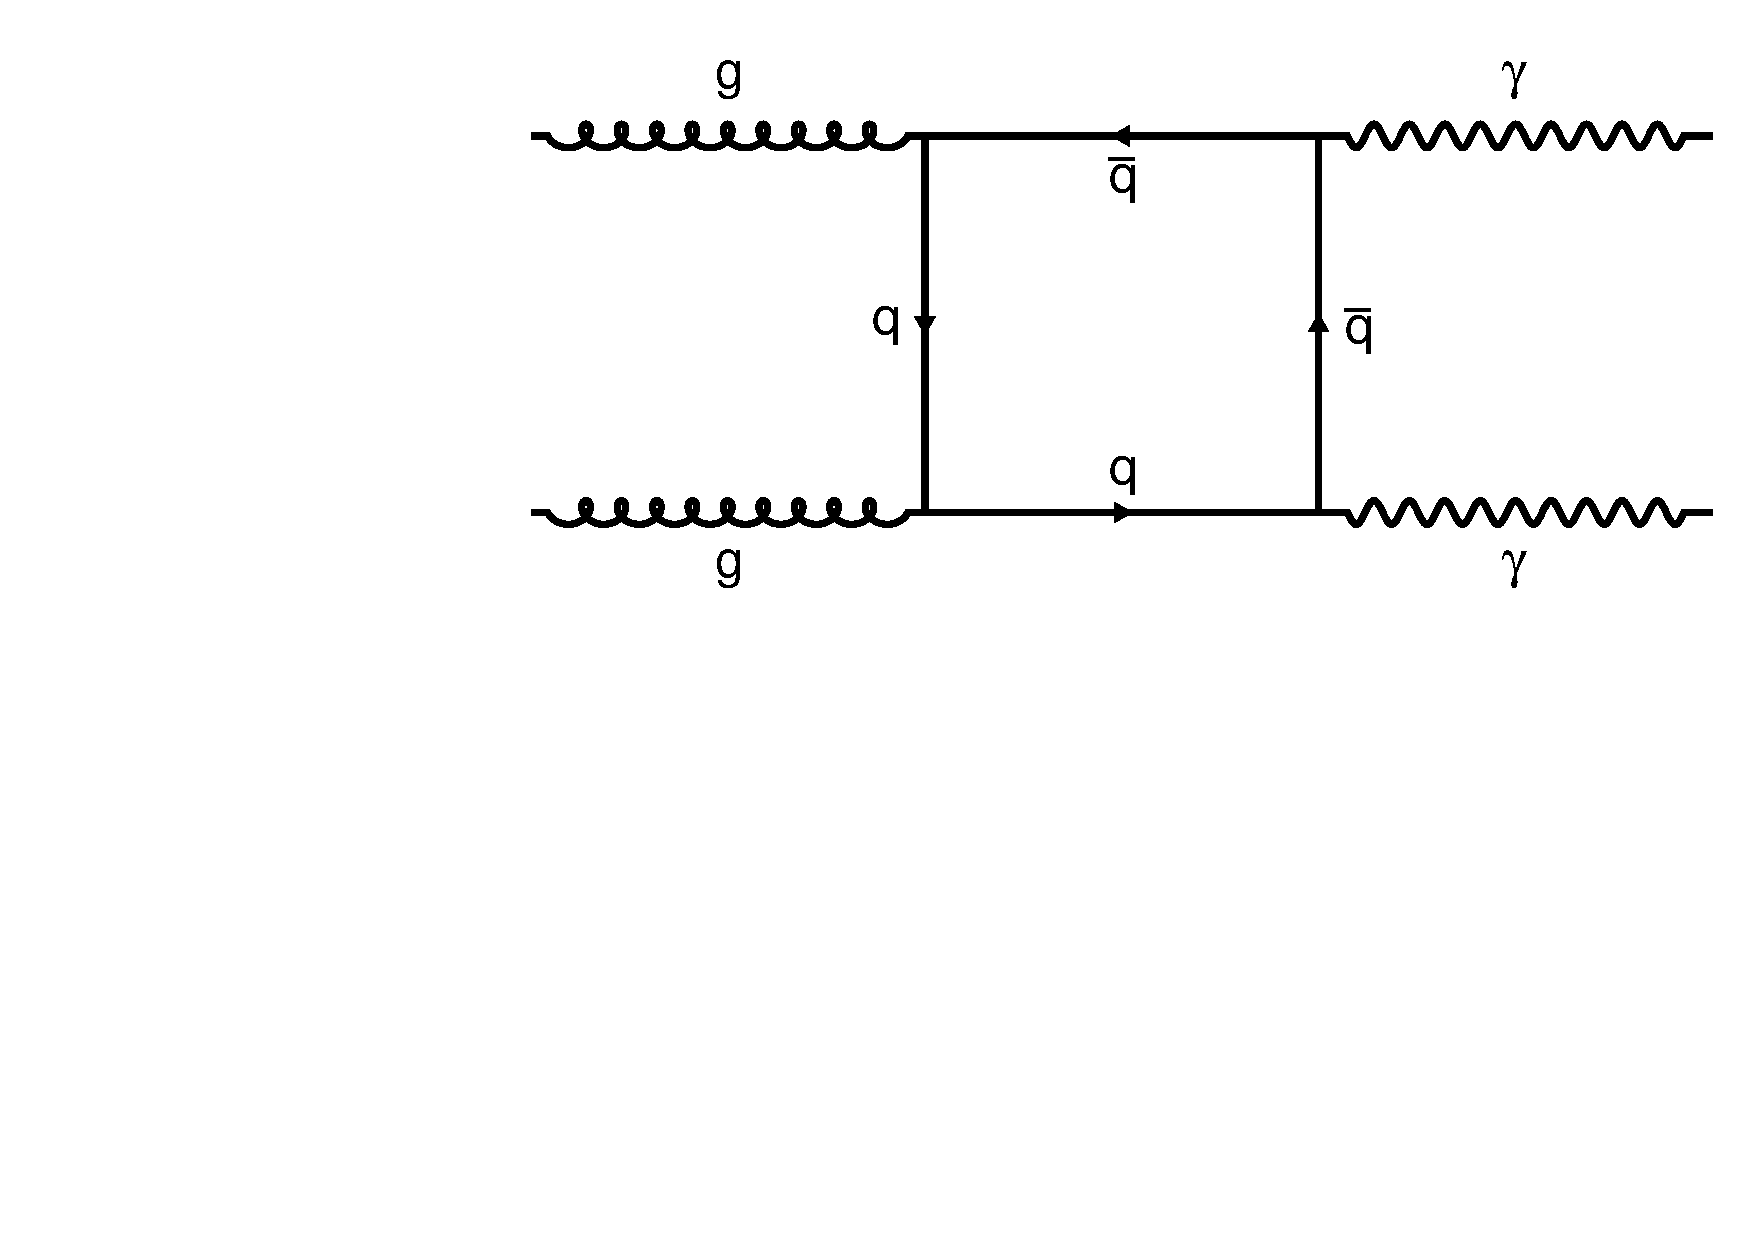
\includegraphics[width=0.32\textwidth]{theory/plots/Box.pdf}
  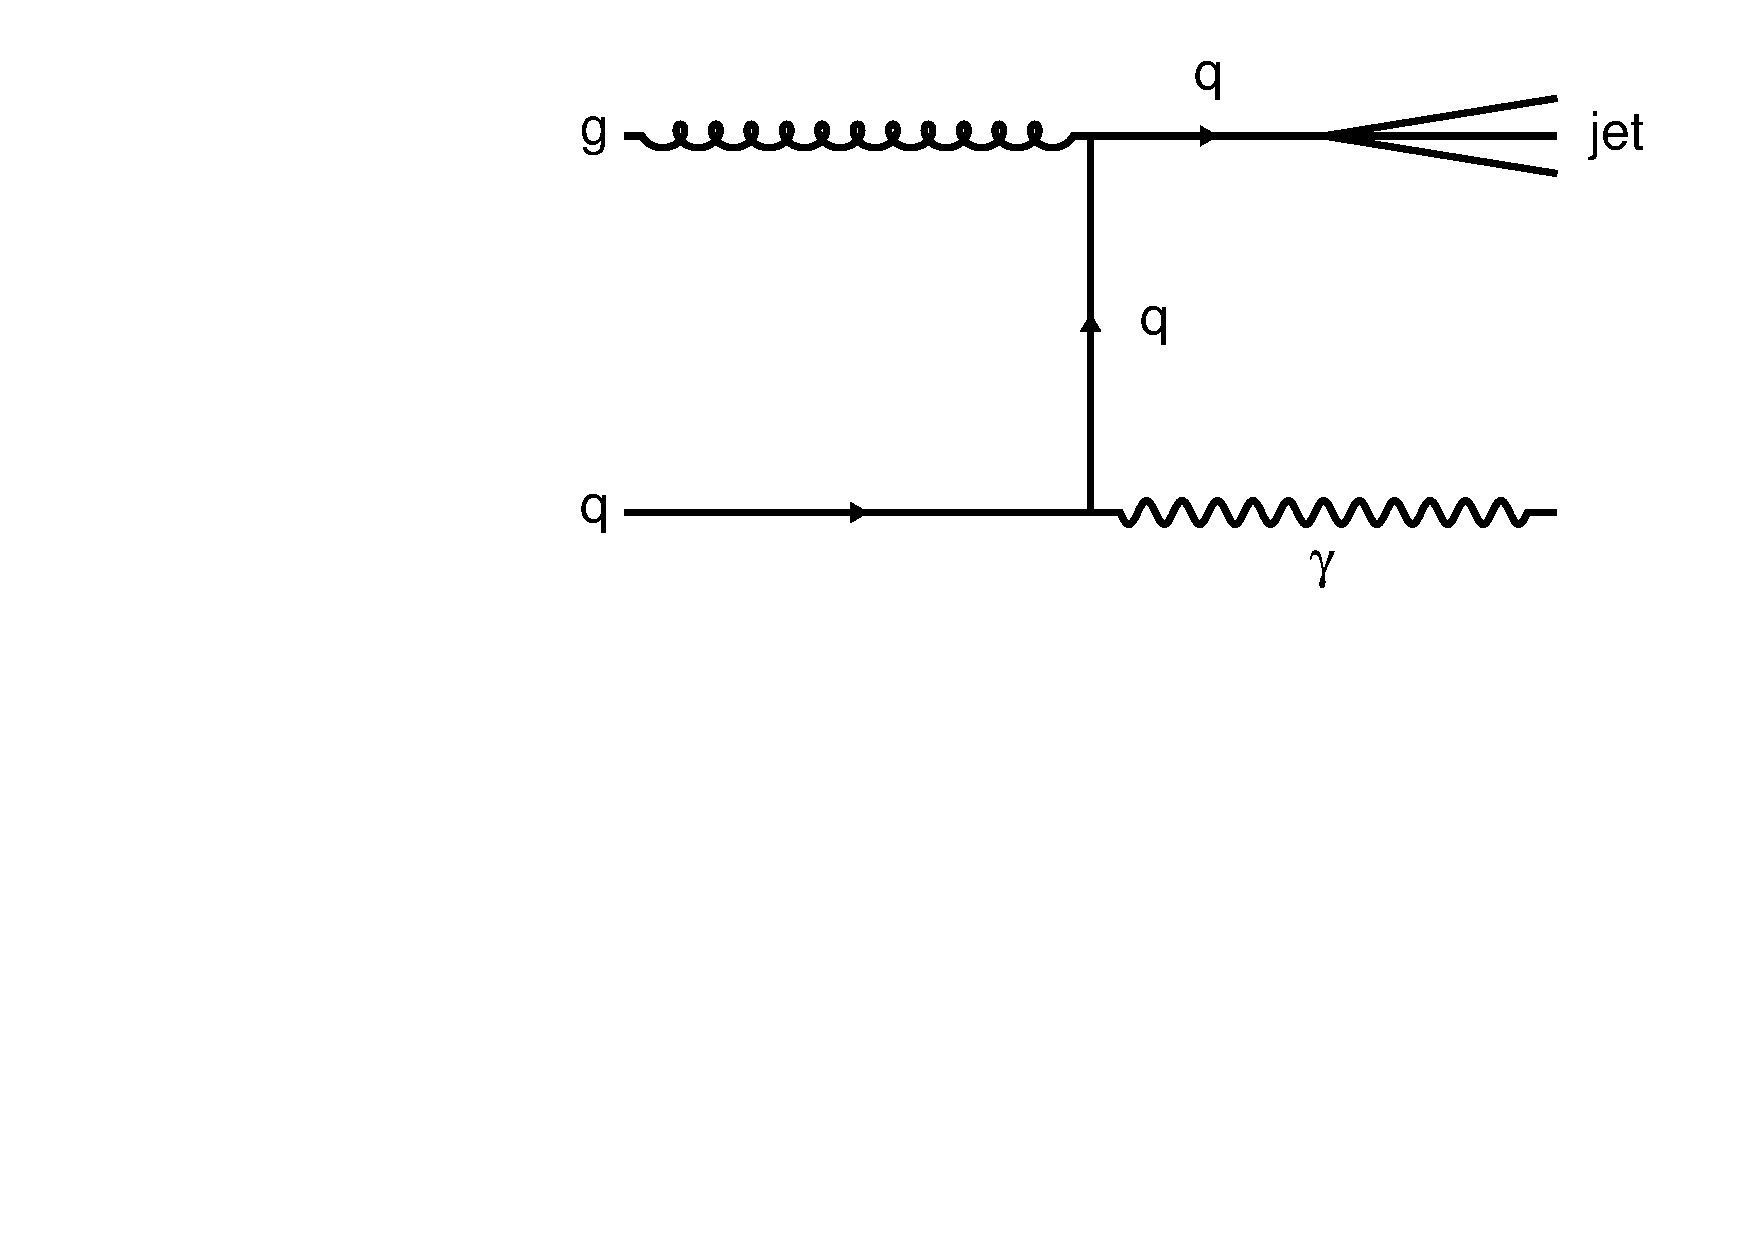
\includegraphics[width=0.32\textwidth]{theory/plots/GJet.pdf}
  \caption[Higgs to two photon backgrounds at the \acs{LHC}]{The prompt-promt and prompt-fake Feynman diagrams contributing to the \Hgg background via the Born mode (left), box mode (middle) and \gjet mode (right).}
  \label{fig:feyn_bkgs}
\end{figure}

One of the most important variables used in the analysis is the invariant mass of the two photons, which for signal is equivalent to the reconstructed Higgs mass. The invariant mass distribution for background is expected to be a smoothly falling continuum whereas the signal is expected to be a narrow resonance centred at the Higgs mass. The difference between these is heavily exploited in the analysis. The diphoton invariant mass is reconstruced using,
\begin{equation}
	m_{\gamma\gamma} = \sqrt{2E_{\gamma1}E_{\gamma2}(1-\cos(\alpha))},
\label{eq:invmass}
\end{equation}
where $E_{\gamma1}$ and $E_{\gamma2}$ are the energies of the two photons, and $\alpha$ is the angle between them.

The remainder of this thesis will concentrate on the details of an analysis of Higgs events decaying into two photons at the \CMS experiement at the \LHC. Many of the features discussed in the last section will be exploited using sophisticated computing, analysis and statistical techniques which ultimately culminate in a standalone observation of a resonance near 125~\GeV and subsequent measurements of this particles properties.


  \chapter{The CMS experiment}
\label{chap:cms}
\chapterquote{You need something to open up a new door, \\
To show you something you seen before, \\
But overlooked a hundred times or more.}
{Bob Dylan}

\section{The LHC}

The \LHC is an octagonal 27km ring (large) proton-proton (hadron) particle collider. Using a multistage acceleration process two beams of protons are circulated in opposite directions at a centre-of-mass energy in excess of $\sqrt{s}$=7~TeV. The protons are sourced from Hydrogen and circulate the collider in bunches.  


The \LHC ring consists of eight straight line segments, in which the charged beams are accelerated by an oscillating electric field using radio frequency (RF) cavities, and eight arc segments, which are filled with superconducting magnets whose effect is to circulate the beam of protons around the ring. The average spacing between bunches is 50~ns for the data used in this thesis, although the \LHC can operate at a bunch spacing of 25~ns, and there are about 100 million protons per bunch. Precision magnetic fields can control the position and intensity of the beams such that they can be focused into a small space (around 64 microns at the interaction point) and collided together. The result is about 20 collisions per crossing. For the data used in this thesis the \LHC operated at centre-of-mass energies of $\sqrts=7$ and 8~TeV. 

There are four points around the ring where the beams can be forced to intersect producing high energy proton-proton collisions. Particle detectors are constructed around these points such that the collision can be reconstructed with the purpose of measuring physical properties and processes, calibrating the detectors with already known processes and searching for new physics. The remainder of this chapter concentrates on a description of one of these detectors, \CMS, which the author has worked on.

\section{The CMS detector}

The \CMS detector, pictured in Fig.~\ref{fig:cms_diagram}, is a multipurpose experiment designed for the measurement of and search for a multitude of different processes. We will primarily discuss its function as a Higgs finding machine. A more detailed description can be found in Ref.~\cite{CMS_JINST}. It has a cylindrical shape consisting of a barrel segment, 21.6~m long, and two endcaps, 14.6~m in diameter, aligned along the beam direction with its centre at the beam interaction point. The endcaps are nearer the beam line and so the materials in these components typically have to be able to withstand higher amounts of radiation and therefore tend to have worse performance. Many of the features of \CMS exploit what one would expect for measuring Higgs decays: it has almost full coverage of the area around the collision point so that nearly every particle emanating from the collision can be reconstructed and it has many complimentary subsystems (or layers) designed to measure different specific particles so that Higgs bosons can be detected through a multitude of decay modes. 

\begin{figure}
  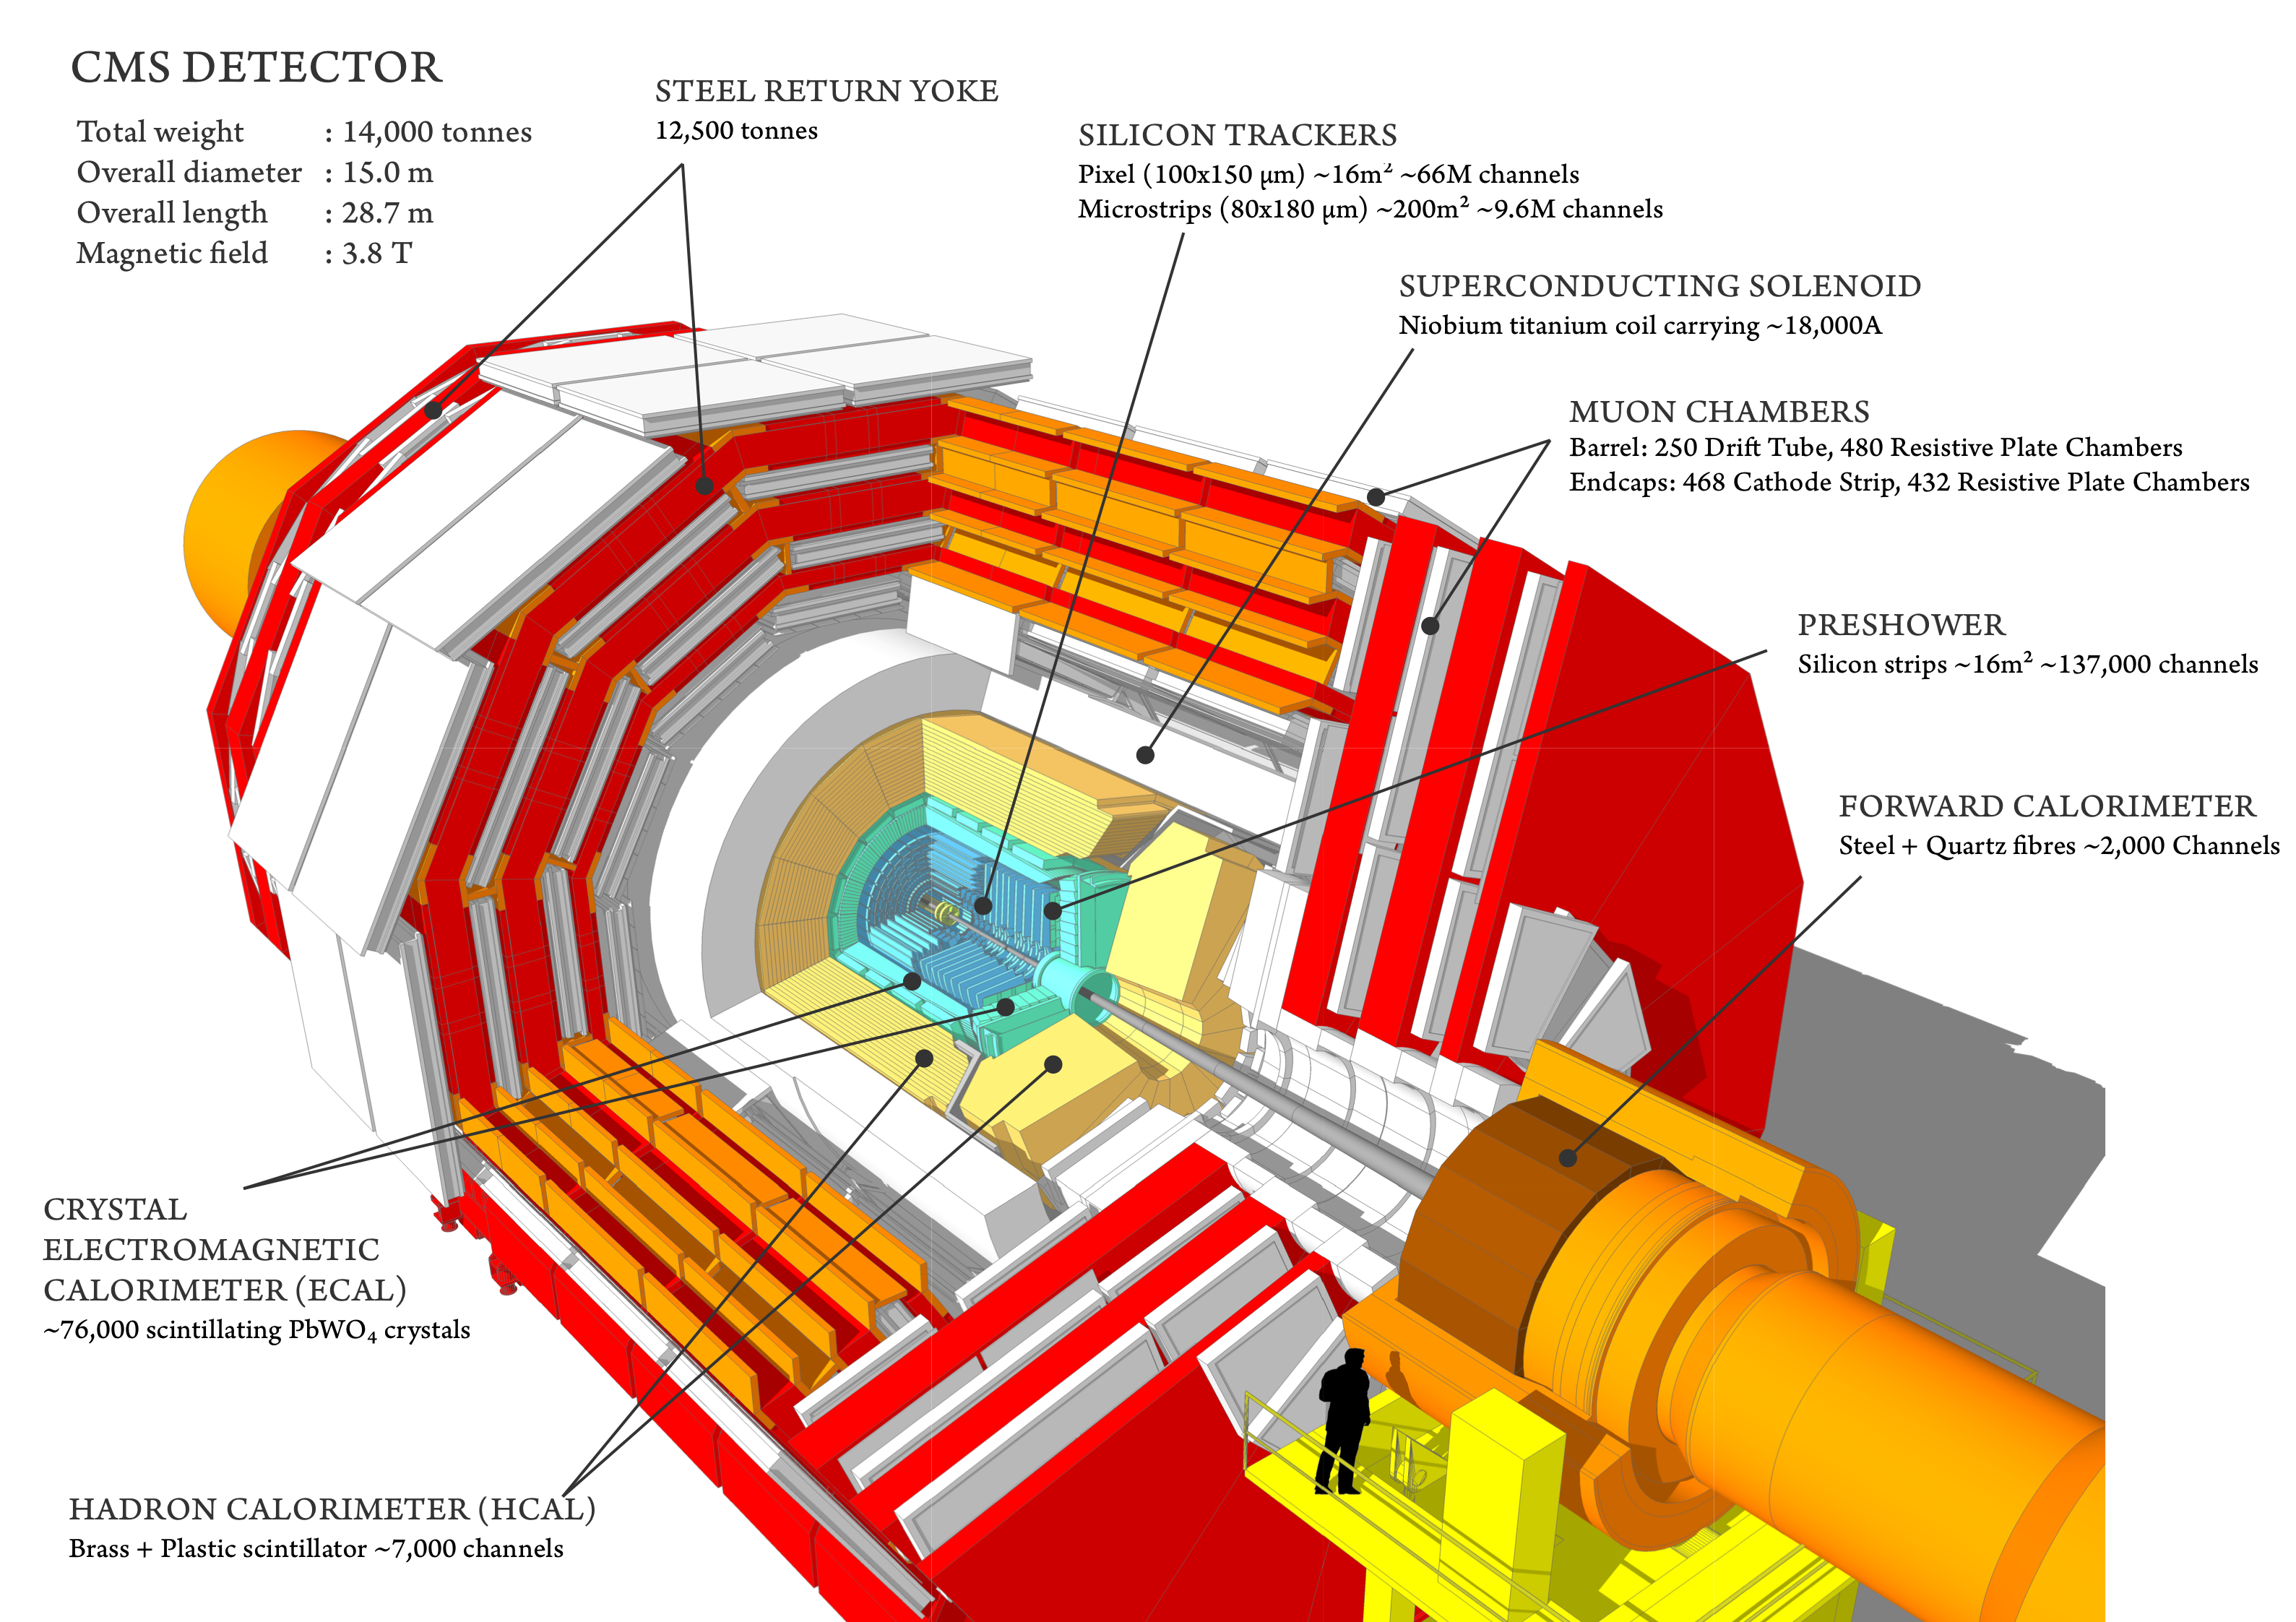
\includegraphics[width=0.8\textwidth]{cms_experiment/plots/cms_diagram.png}
  \caption[\acs{CMS} diagram]{This is a schematic representation of \CMS showing the layered structure of subdetectors; tracking system, calorimeters, magnet and muon system.}
  \label{fig:cms_diagram}
\end{figure}


For a Higgs with an intermediate mass ($100 - 200$~\GeV) the high resolution (narrow peak) channels are $H\rightarrow ZZ^{*}$ \footnote{A $^{*}$ denotes that one $Z$ can be off mass shell} $\rightarrow l^{+}l^{-}l^{+}l^{-}$ and \Hgg so good energy resolution and identification of electrons and muons is desirable down to very low \pT ($\sim O(10$\GeV)) as well as good resolution and identification of high energy photons. 

The central design feature of \CMS is the very powerful superconducting magnet which produces an axial magnetic field of 4T. The size of this field, as well as the density of the calorimeter materials, allows for a compact and economical design (much more so than its sister detector, ATLAS). Outside of the magnet lie the muon stations which also serve as a return yoke for the magnetic field. The muon chambers in the barrel consist of alternating layers of drift tubes and resistive plate chambers which provide both accurate timing and hit location, in order to reconstruct muons down to low energies. In the endcap the drift tubes are replaced with cathode strip chambers. Combining information from the muon subsystem with information from the inner tracking system (described below) allows muons at \CMS to be reconstructed down to $p_{T}<10$~GeV with a resolution of $\sim1\%$. The other three main subsystems at \CMS, the tracking system and the two calorimeters, are located inside the magnet

The first layer, moving outwards from the interaction point, is the tracking system which is used to reconstruct the momentum of any outgoing charged particles and to locate the primary and secondary vertices. This is surrounded by the calorimeters, the \ECAL and the \HCAL. The first is a single layer of dense, transparent crystals which collects deposits of energy left by electrons and photons which shower inside the material. The second compliments this by providing a measurement of the energy deposited by hadrons (reconstructed as objects known as jets) through nuclear interactions. The \HCAL is a sampling calorimeter in which the active material (plastic scintillator) is sandwiched between a dense absorbent material (brass or steel). This extends the radiation length of the calorimeter (clearly accommodating the compact design) and provides pointing information but degrades the resolution of reconstructing jets. 

\CMS uses a right-handed Cartesian coordinate system with the origin at the interaction point and the $z$-axis pointing along the beam line. The $x$-axis points towards the centre of the \LHC ring and the $y$-axis points vertically upwards. The azimuthal angle, $\phi \in [-\pi,\pi]$, is defined with respect to the $x$-axis in the transverse $(x-y)$ plane. The polar angle $\theta$ is measured from the $z$-axis. Commonly, the direction of an outgoing particle is defined by $\phi$ and its pseudo-rapidity $\eta$,
\begin{equation}
	\eta = -\ln\tan\biggl(\frac{\theta}{2}\biggr).
\end{equation}
The \LHC is capable of producing 40M bunch collisions per second, and each can result in several $p$-$p$ collisions, although many of these are not hard interactions, the result being that the outgoing particle debris follows the beam line. A hard (and therefore interesting) collision is characterised by the amount of energy produced in the transverse ($x-y$) plane. Therefore particles are commonly characterised by the projection of their momentum onto this plane, their transverse momentum,
\begin{equation}
	p_{T} = \sqrt{p_{x}^{2}+p_{y}^{2}},
\end{equation}
and the corresponding transverse energy, $E_{T} = E\sin(\theta)$.

% --------- TRACKER ----------
\subsection{Tracking system}
\label{sec:tracker}

During nominal \LHC running conditions in 2012 there are on average over 1000 particles from up to 50 overlapping \pp collisions (pileup) per bunch crossing (every 50 ns). The tracker is designed to efficiently and precisely reconstruct all charged particle trajectories, and thus their position and momentum, which are known as tracks. Due to the vast number of tracks emanating from multiple vertices in typical \LHC collisions, the tracking material and electronics are required to have high granularity, a fast response and be radiation hard. This conflicts with another important design feature of the tracker which is the aspiration to use the minimal amount of material in order to reduce multiple scattering, bremsstrahlung, photon conversion and nuclear interactions before particles reach the calorimeters. These criteria motivate the choice of silicon throughout the \CMS tracking system. The structure of the \CMS tracker is shown in Fig.~\ref{fig:cms_tracker} and consists of a central pixel detector (PIXEL) surrounded by layers of silicon strips aligned parallel to the beam line in the barrel (TIB and TOB) and perpendicular to the beam line in the endcap (TID and TEC). The total active surface of the tracking system is about 300~m$^{2}$ and is intrumented with 12$\times10^{6}$ channels~\cite{tracker_project}.

By making multiple precise measurements of tracks as they pass through the pixel and silicon layers the track trajectories can be reconstructed and their momentum calculated using their curvature in the \phi plane due to the axial magnetic field. Tracks are grouped together (requiring that their separation is less than 1~cm in the $z$ coordinate at the point of closest approach to the beamline) and assigned to a common point or origin (the primary vertex). The vertex resolution is driven both by the number of tracks originating from a particular vertex and how large their average \pT is. This is shown in Fig.~\ref{fig:tracker_vertex_resolution} for preliminary data taken in 2010 at $\sqrt{s}=7$~TeV.

\begin{figure}
  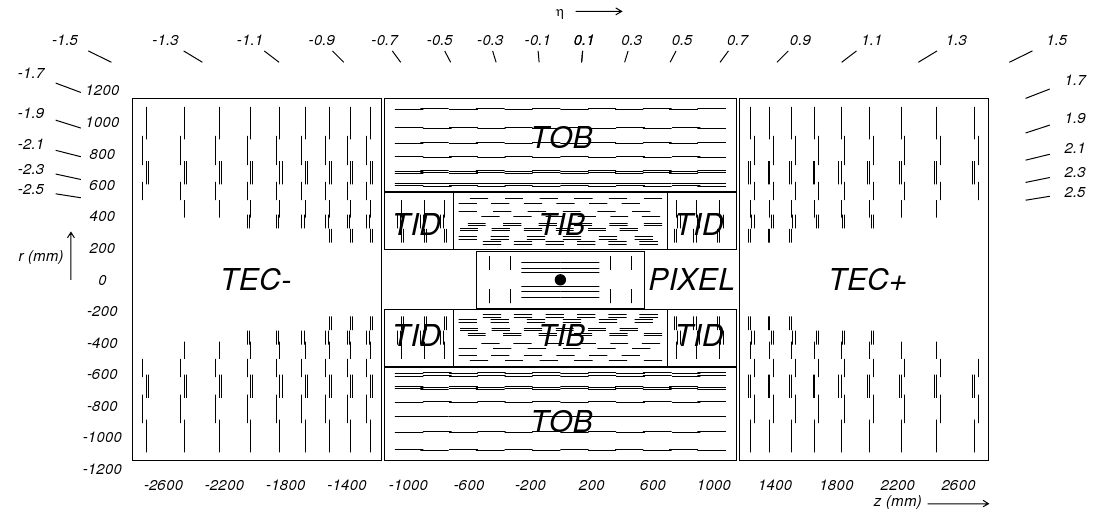
\includegraphics[width=0.9\textwidth]{cms_experiment/plots/fig_cmstracker.png}
  \caption[\acs{CMS} tracker]{A diagram of the \CMS tracking system showing the PIXEL detector and outer silicon strip layers~\cite{CMS_JINST}.}
  \label{fig:cms_tracker}
\end{figure}

\begin{figure}
  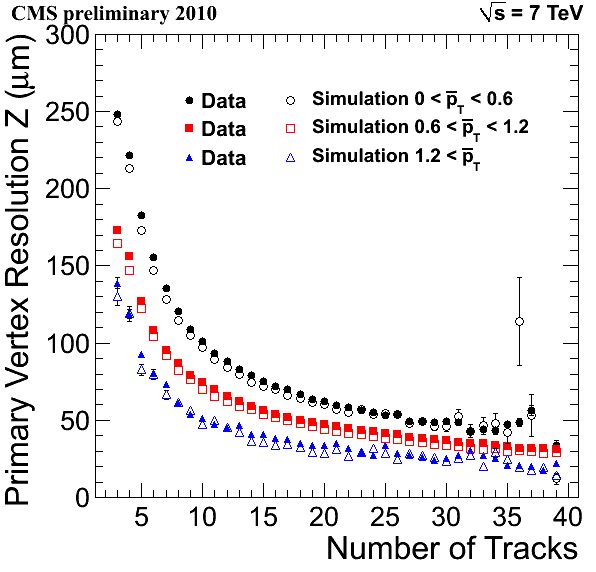
\includegraphics[width=0.48\textwidth]{cms_experiment/plots/ResZ_byPt.png}
  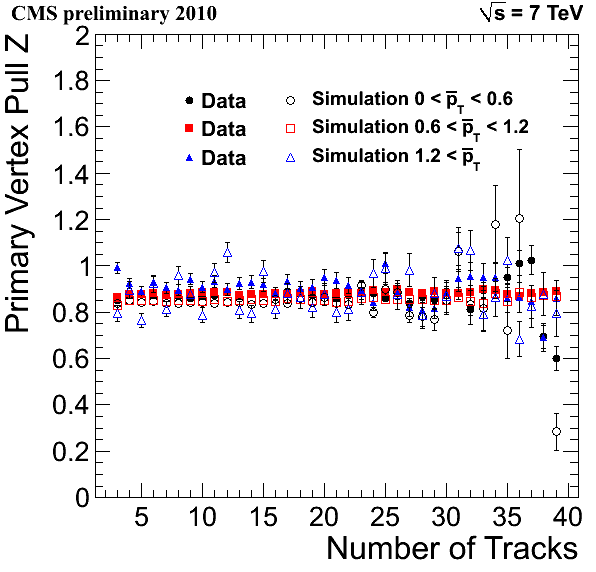
\includegraphics[width=0.48\textwidth]{cms_experiment/plots/PullZ_byPt.png}
  \caption[Vertex resolution]{A demonstration of the vertex position resolution in Z as a function of the number of tracks originating from that vertex. The different colours respresent three different bins in the average track \pT where data is shown as solid points and simulation as open points~\cite{cms-tracker-performance-2010}.}
  \label{fig:tracker_vertex_resolution}
\end{figure}

The amount of material in the tracking system is shown in Fig.~\ref{fig:tracker_material} which demonstrates as a function of \eta which subsystems of the tracker, beam pipe and servicing contribute to material inbetween the interaction point and the calorimeters in radiation lengths (X$_{0}$) and nuclear interaction lengths ($\lambda_{I}$). As shown in Fig.~\ref{fig:cms_tracker} the tracker has full coverage in \phi and up to $|\eta|\leq2.5$. As we will see later the tracking system is very important for the \Hgg search at \CMS as without it locating the primary vertex would be practically impossible.

\begin{figure}
  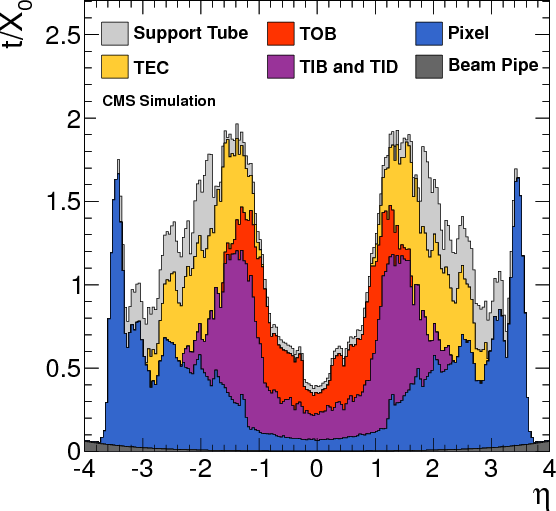
\includegraphics[width=0.48\textwidth]{cms_experiment/plots/tracker_material.png}
  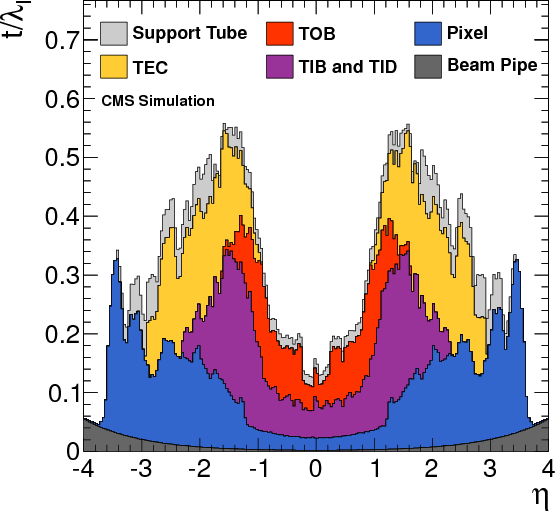
\includegraphics[width=0.48\textwidth]{cms_experiment/plots/tracker_material_lambda.png}
  \caption[\acs{CMS} tracker material budget]{The amount of \CMS tracker material in radiation lengths (X$_{0}$) on the left and in nuclear interaction lengths ($\lambda_{I}$) on the right as a function of $\eta$ for the different tracking subsytems~\ref{tracker_material}.}
  \label{fig:tracker_material}
\end{figure}

% --------- ECAL SECTION ----------
\subsection{Electromagnetic calorimeter}
\label{sec:ecal}
The \ECAL is used to reconstruct the energy of electrons and photons which deposit their energy via electromagnetic showers inside the calorimeter material. The shower inside the crystal produces photons whose total energy is proportional to the energy of the incoming particle. Hence the light output from the shower, which can be measured by photodiodes at the back of each crystal, in turn provides a measurement for the energy of the original particle. The \ECAL has almost full hermetic coverage of the interaction point and consists of a single layer of \PbWO crystals. The crystals are laid out in a quasi-projective geometry such that they point towards the interaction point with an offset of 3$\degree$ making it much less likely that a photon, or electron, will pass straight through a gap between crystals. The \ECAL consists of a barrel section and two endcap disks which are preceded by a preshower (to aid with \pizero rejection), a schematic is shown in Fig.~\ref{fig:cms_ecal}. There is a fiducial region between the barrel and endcap (to prevent reconstruction of showers which overlap both subsystems) yielding an \ECAL coverage of $|\eta|<2.5$ but not in the range $1.444<|\eta|<1.556$ and full coveraege in \phi. Typical crystal dimensions are ~$2.2\times 2.2$cm at the \ECAL face, with a depth of 23~cm (which amounts to 25.8~X$_{0}$) implying that practically the whole depth of the shower is contained within this single layer~\cite{ecal_project}. 
\begin{figure}
  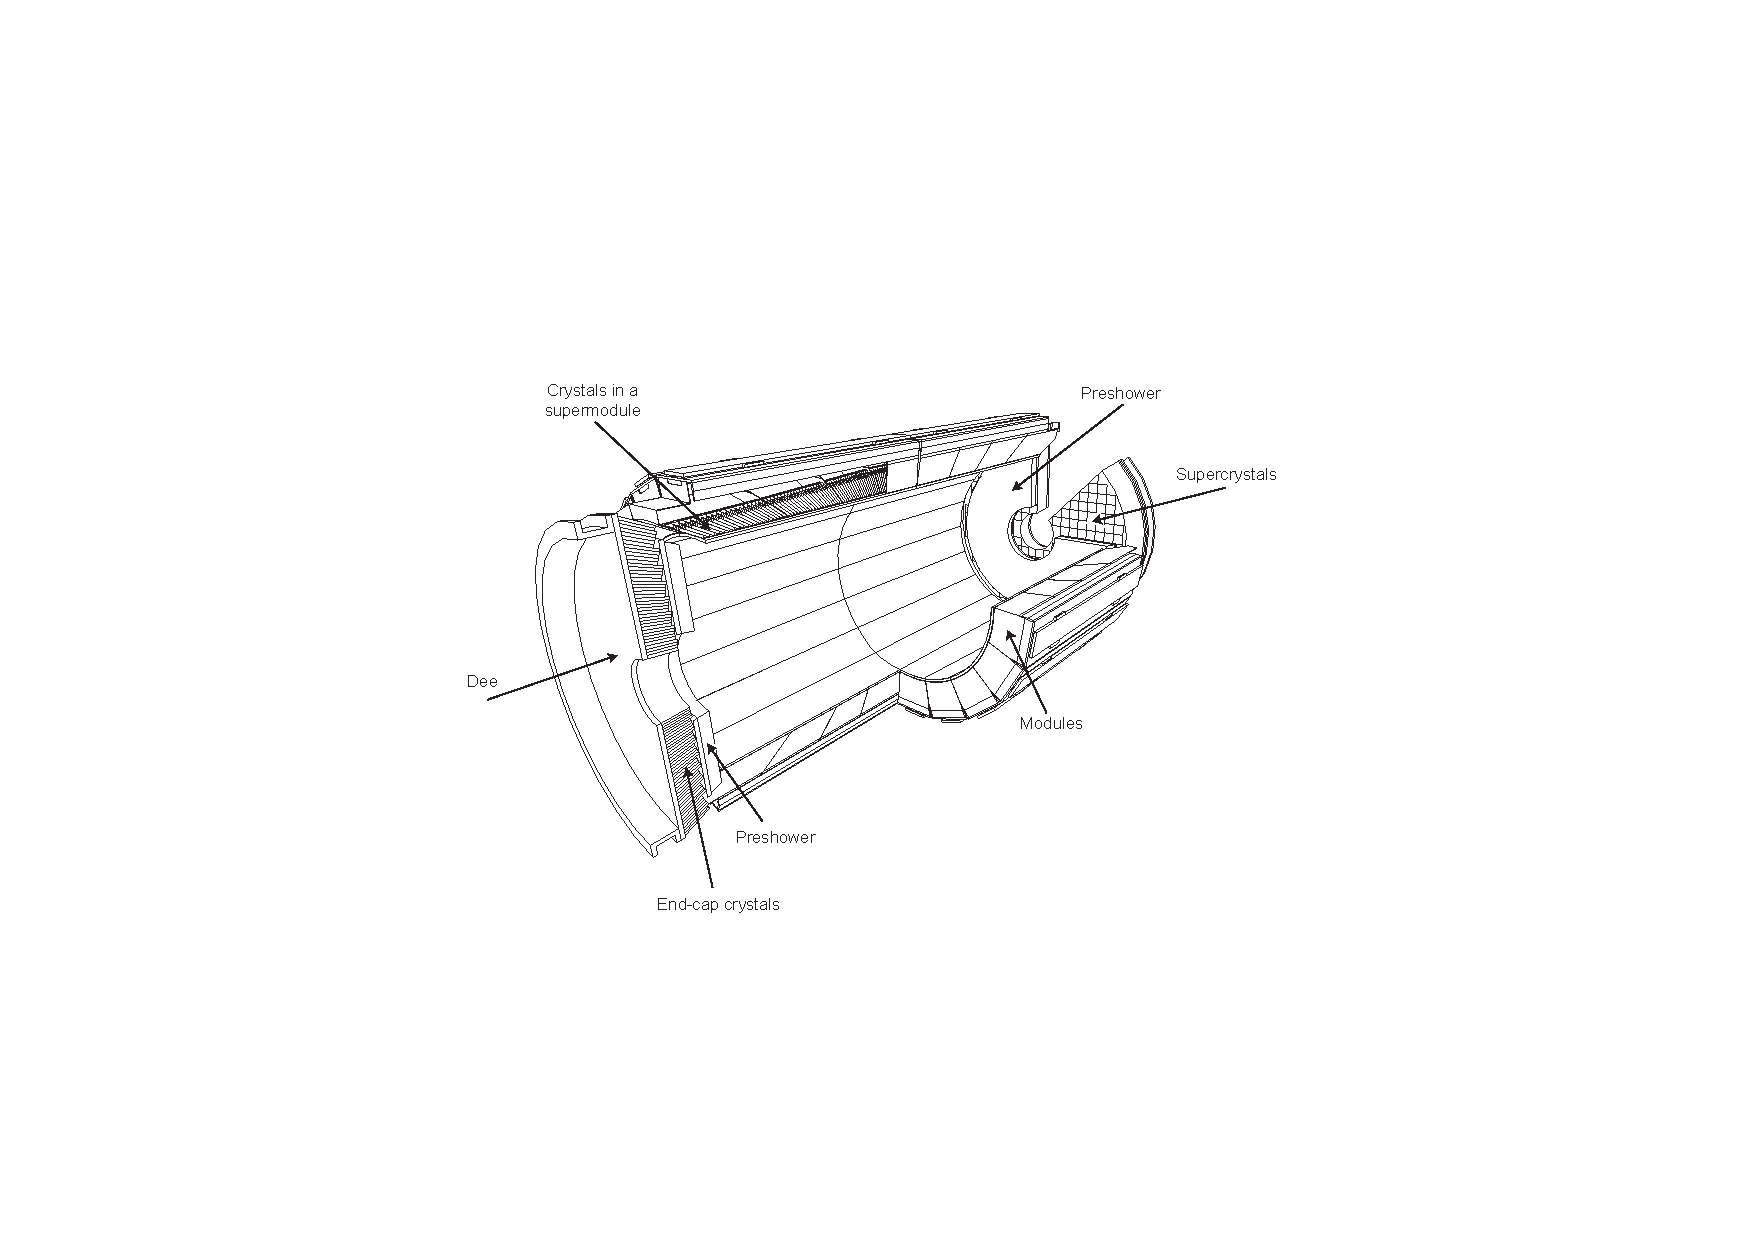
\includegraphics[width=0.7\textwidth]{cms_experiment/plots/cmsecal.pdf}
  \caption[\acs{CMS} \acs{ECAL} schematic]{A schematic drawing of the \CMS \ECAL layout showing the ``modules" of crystals in the \ECAL barrel and the ``Dees" of crystals in the \ECAL endcap~\cite{CMS_JINST}.}
  \label{fig:cms_ecal}
\end{figure}

\PbWO has some attractive properties for an electromagnetic calorimeter especially when considering \Hgg decays. In order to acheive good energy resolution it is desirable to have a design in which most of the electromagentic shower from an incoming photon or electron is contained within a single crystal, as less of the shower (and therefore energy) is lost in cracks and gaps in-between crystals. \PbWO has a short radiation length ($X_{0}=0.89$~cm), which compliments a compact design as the entire depth of the shower can be contained in a crystal which is not very long, and it has a small Moli\`{e}re radius (1.96~cm) which means that the lateral size of the shower is small. This generally means that the cross-sectional size of a crystal can be small (yielding high granularity of the detector) whilst still containing a large percentage of the shower. It has a very short scintillation time decay constant (85\% of the light is collected in 25~ns), in other words it is very ``fast", allowing the energy in the shower to be collected and measured very quickly. This is clearly desirable in an environment like the \LHC when collisions are happening up to every 25~ns. One draw back of \PbWO (apart from expense) compared to other crystal materials is its relatively low light yield at room temperature ($\sim$50-80 photons/MeV). This is overcome at \CMS with the use of silicon \APDs in the ECAL barrel and \VPTs in the endcap, which amplify the signal enough to make accurate measurements of the original photons energy. 
\subsubsection{Energy resolution}
As we have seen previously the diphoton invariant mass is given by,
\begin{equation}
  m_{\gamma\gamma} = \sqrt{2E_{1}E_{2}(1-\cos\alpha)},
  \label{eq:dipho_inv_mass}
\end{equation}
where $E_{1}$ and $E_{2}$ are the energy of the two photons and $\alpha$ is the angle between them. Therefore the mass resolution has terms that depend on the photon energy resolution and angular resolution,
\begin{equation}
  \frac{\sigma_{M}}{M} = \frac{1}{2} \Biggl[ \frac{\sigma_{E_{1}}}{E_{1}} \oplus \frac{\sigma_{E_{2}}}{E_{2}} \oplus \frac{\sigma_{\alpha}}{\tan(\alpha/2)} \Biggr],
  \label{eq:mass_res}
\end{equation}
where $\sigma$ denotes the resolution and $\oplus$ the quadratic sum. It is therefore desirable to have both good energy resolution and good position resolution for photons (accurate position measurements at the \ECAL face alongside knowledge of the primary vertex can be used to calculate the individual photons' direction and ergo the angle between them). The energy resolution is usually then further parametrised as,
\begin{equation}
  \frac{\sigma_{E}}{E} = \frac{a}{\sqrt{E}} \oplus \frac{b}{E} \oplus c,
  \label{eq:energy_res}
\end{equation}
where $a$ is the stochastic term, $b$ the noise term and $c$ a constant term. In order to acheive the best possible resolution, all three of these terms need to be of a similar order and as small as possible. The size of these terms has been determined from test beam data in Ref.~\cite{CMS_JINST}. The stochastic term is driven by the material choice and detector type so cannot be improved once the machine is built. The main contributions to this term are lateral shower containment fluctuations, photostatistics and fluctuations in the energy deposited in the preshower absorber. For a fully active calorimeter (the \CMS \ECAL is not a sampling calorimeter) made of \PbWO the size of this term is good ($a=0.028\pm0.003~$GeV$^{\frac{1}{2}}$). The constant term, which depends on non-uniformity of longitudal light, intercalibration errors and energy leakage from the back of the crystal, can be minimzed by use of \emph{in situ} calibration of individual crystals and amounts to $c=0.26\pm0.05\%$. The noise term which has contributions from electronics noise (including signal digitisation) and event pile-up (additional particles causing overlapping signals) is measured as $b=126$MeV. The ECAL energy resolution, $\sigma_{E}/E$, as a function of electron energy is shown in Fig.~\ref{fig:sigma_e_test_beam} as measured from a beam test~\cite{CMS_JINST}. 
\begin{figure}
  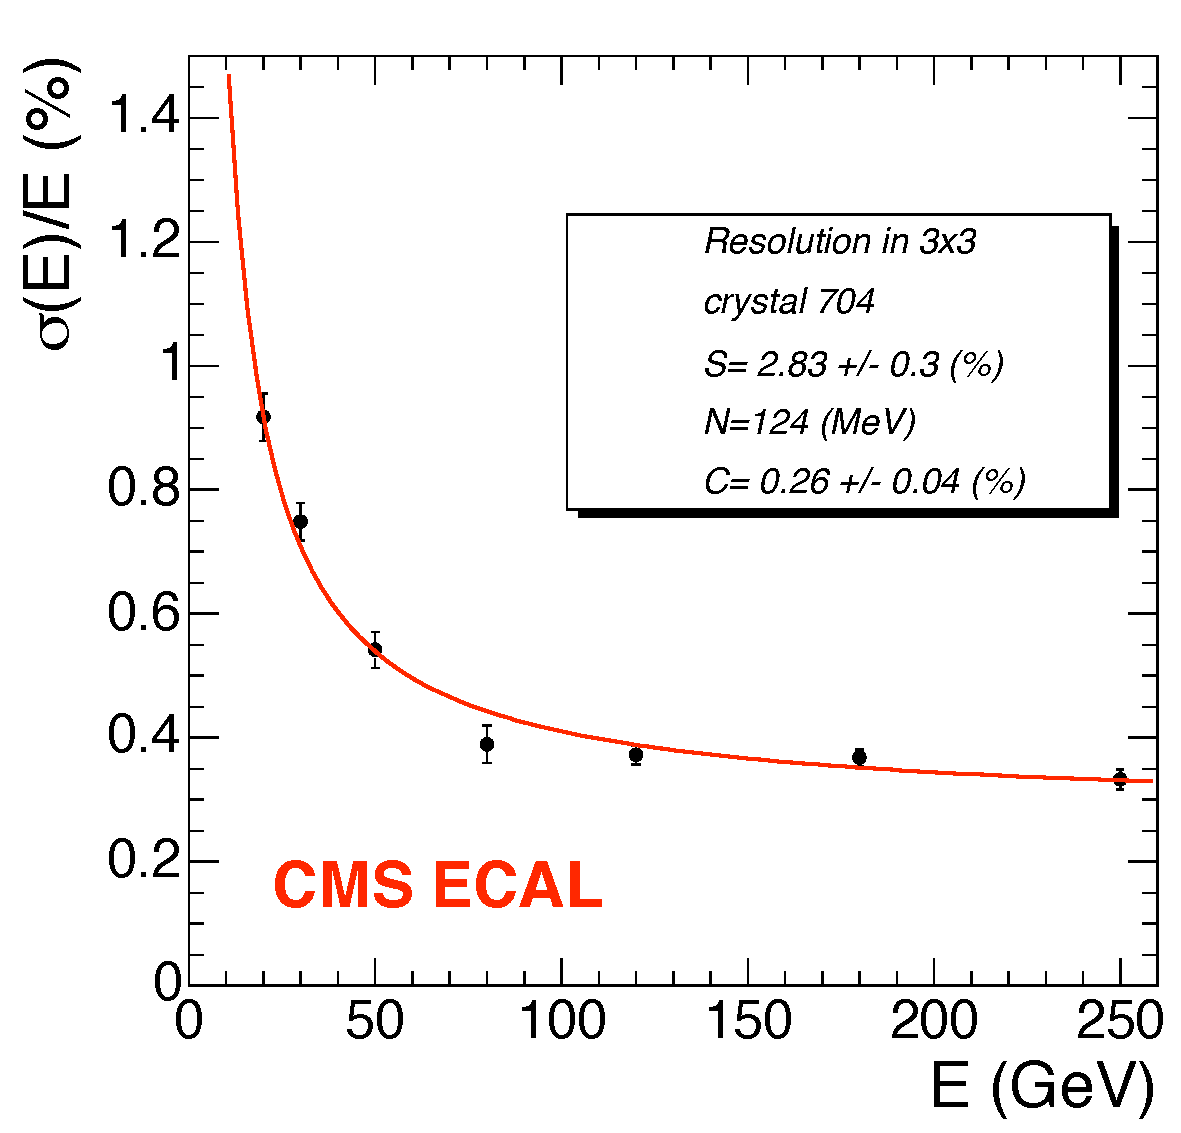
\includegraphics[width=0.6\textwidth]{cms_experiment/plots/ecal_sigma_e_test_beam.pdf}
  \caption[\acs{ECAL} energy resolution]{The \ECAL energy resolution, $\sigma_{E}/E$, as a function of electron energy measured from test beam data. The energy is measured in a 3$\times$3 array of crystals centered on the crystal of electron impact~\cite{CMS_JINST}.}
  \label{fig:sigma_e_test_beam}
\end{figure}
\subsubsection{Transparency corrections}
Due to the high particle flux present at \CMS the \ECAL crystals and electronics have to be radiation hard, especially in the endcap. This is another motivating factor for using \PbWO as the crystal material. The crystals are additionally doped with Nb to improve the induced absorption coefficient. Over time and long exposure to radiation the crystals lose their transparency, although there is considerable natural recovery during down periods. An important part of the \ECAL monitoring and calibration comes in the form of transparency corrections to compensate for these losses. At regular intervals during \LHC running laser pulses are injected into the crystals to measure the crystal response. Two different wavelengths of laser are used, one blue ($\lambda=440$~nm) which is very similar to the scintillation emission peak and therefore expected to be affected by transparency changes in a similar way to typical scinitillation light, and one red ($\lambda=796$~nm) which is far from the scinitillation emission peak and affected very little by the changes in transparency. Hence, by comparing the red and blue laser light response, time and $\eta$ dependent corrections for crystal transparency loss can be calculated. A closure test for these corrections, in 2012 data, is shown in Fig.~\ref{fig:ecal_laser_corrs} which shows the ratio of electron energy (calculated from the \ECAL) to electron momentum (calculated from the tracker) before and after transparency (or laser) corrections. 
\begin{figure}
  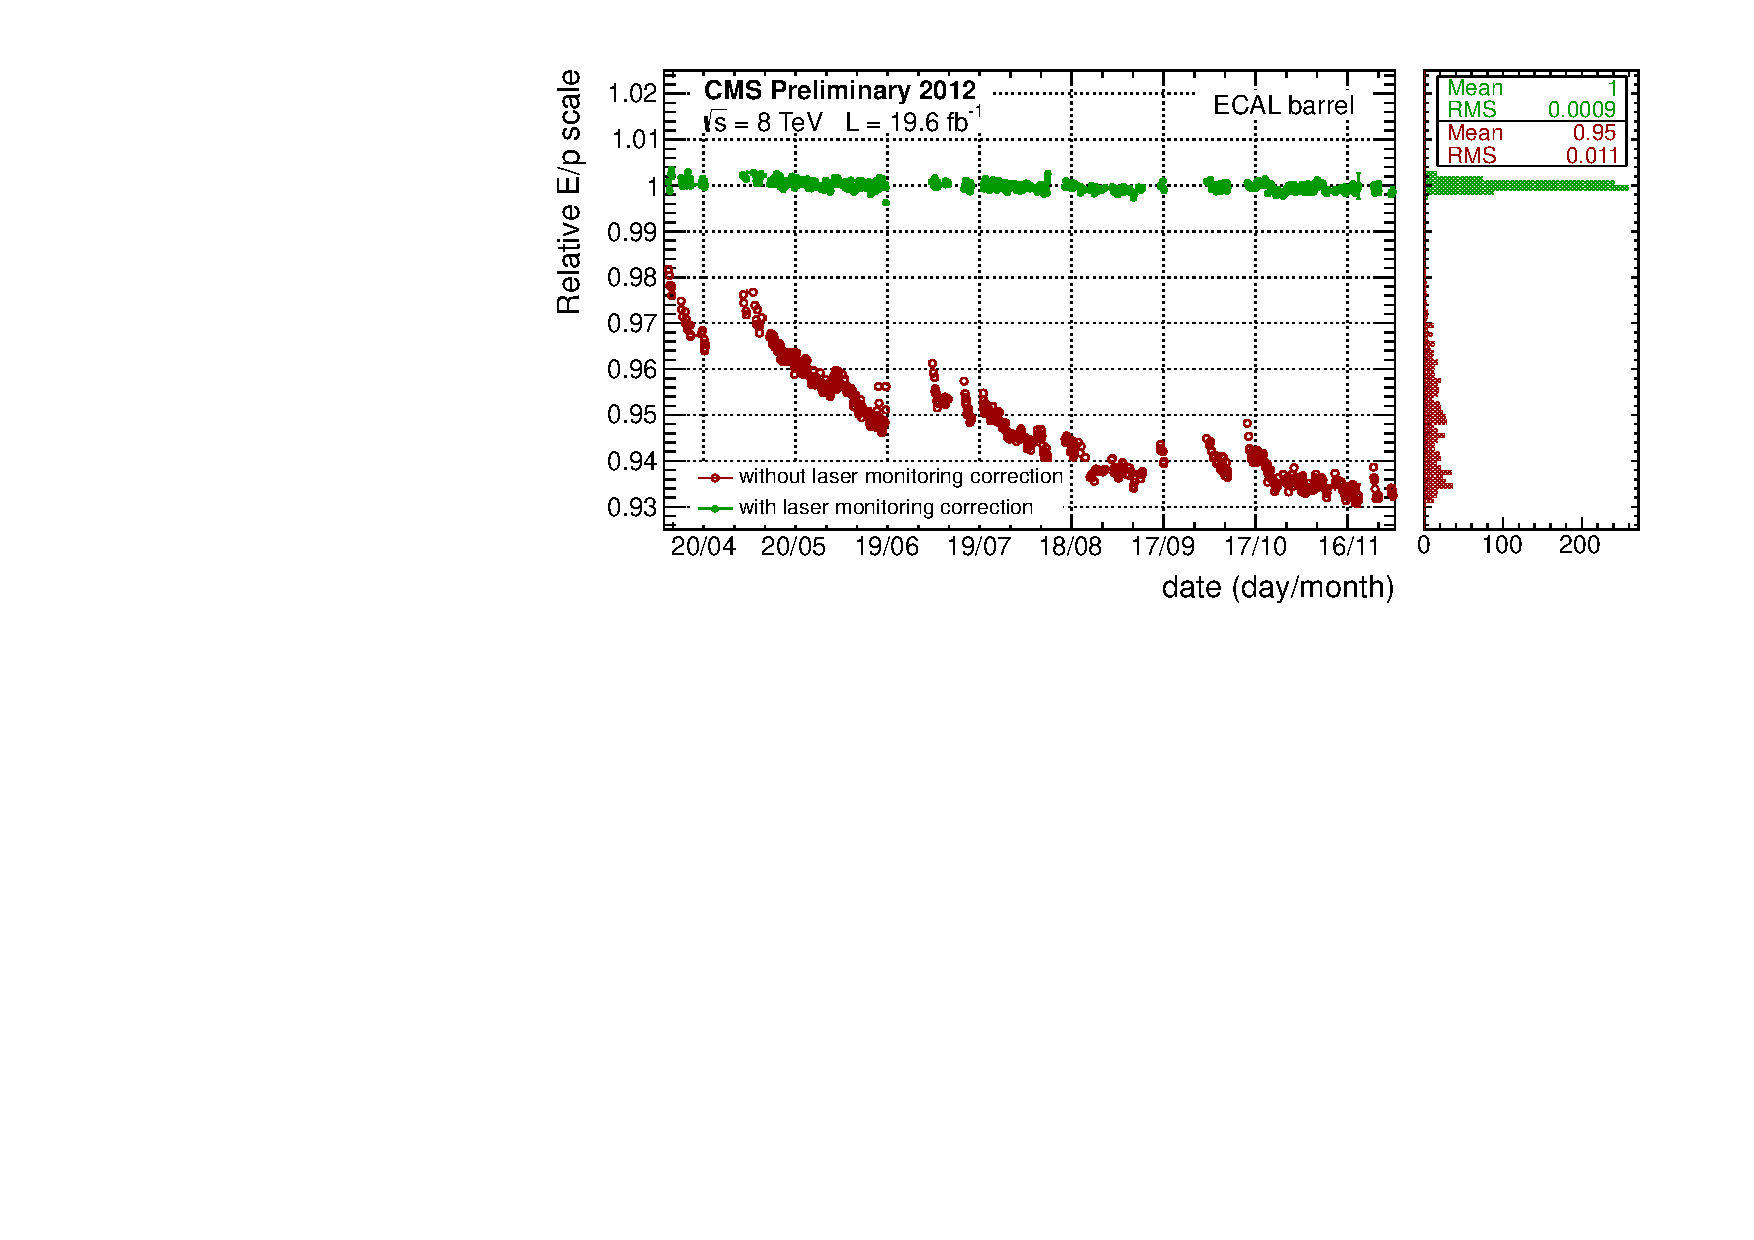
\includegraphics[width=\textwidth]{cms_experiment/plots/ecal_EB_lasercorrs.pdf} \\
  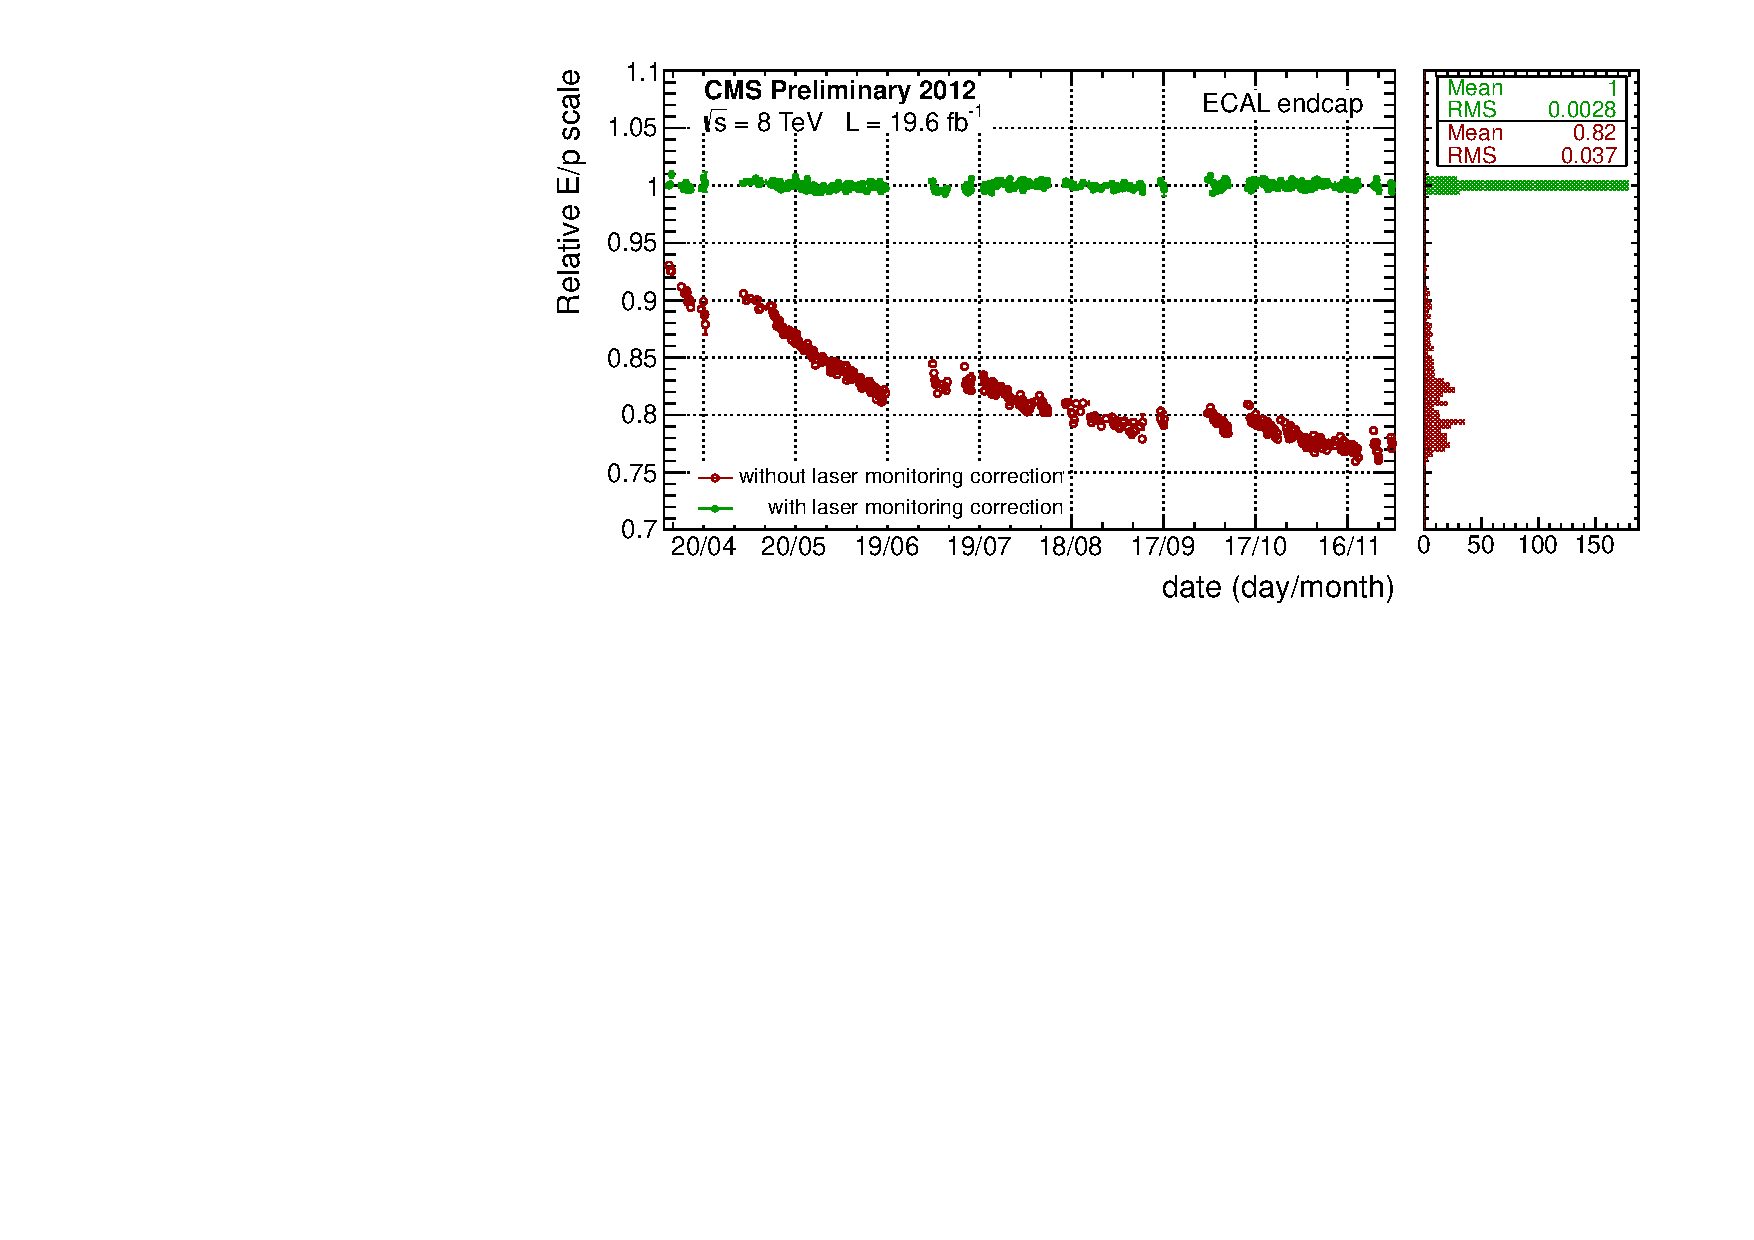
\includegraphics[width=\textwidth]{cms_experiment/plots/ecal_EE_lasercorrs.pdf} 
  \caption[\acs{ECAL} laser corrections]{Ratio of the electron energy, $E$, to the electron momentum, $p$, measured in the \CMS barrel (top) and endcap (bottom) for 2012 data. The open red (solid green) points show the performance before (after) the laser monitoring derived corrections~\cite{cms-ecal-performance-2012}.}
  \label{fig:ecal_laser_corrs}
\end{figure}
\subsubsection{Preshower}
The dominant source of background to high energy photon signals are neutral mesons, mainly pions (\pizero), which sometimes decay into two approximately collinear photons and can therefore look very much like a single high energy photon. The \ECAL endcap is preceded by a preshower to specifically target this and provide the endcap with a higher granularity. The higher granularity helps to discriminate $\pi^{0}$ decays from direct photons using the spatial separation of the two photons from the $\pi^{0}$. The preshower is a sampling calorimeter which consists of two layers: a lead plate, to initiate the shower, in front of a fine grained silicon detector which has two layers of orthogonal strips. There are many other characteristics of \pizero decays which can help in differentiating them from real (``prompt") photons, these include isolation (discussed later in this Chapter in Sec.~\ref{sec:iso}) and the shower shape (discussed in Chapter~\ref{chap:selection_and_categorisation} in Secs.~\ref{sec:cic} and~\ref{sec:pho_id_mva}).

% --------- HCAL SECTION ----------
\subsection{Hadronic calorimeter}
\label{sec:hcal}

Surrounding the \ECAL, but still inside the magnet, is a sampling \HCAL which has geometric coverage up to $|\eta|<5.0$ when including the specialised forward components. It consists of alternating layers of brass plates and plastic scintillators (where in the very forward region the brass is replaced with steel). The \HCAL thickness constitutes around 10-15 nuclear interaction lengths ($\lambda_{I}$) depending on \eta. Any outgoing hadrons from the interaction (of which there are many for a typical event with high \ET) get reconstructed as objects known as ``jets" by amalgamating information from the tracking system, the \ECAL and the \HCAL. This process, in which individual hadrons are first reconstructed and then collected to form jets, is described in more detail in the particle flow section below (section~\ref{sec:pflow_jets}).  

% --------- Muon system ----------
\subsection{Muon Chambers}
\label{sec:muons}
Outside of the magnet lie the \CMS muon chambers. These consist of alternating layers of drift tube chambers (cathode strip chambers) in the barrel (endcap) and resistive plate chambers which also act as a return for the magentic flux. The muon detector has coverage up to $|\eta|<2.4$ and given the particularly conspicuous signature of muons (several hits in the tracker and hits in each muon station layer) the reconstruction efficiency and momentum resolution of muons is very good even down to low \pT. The muon resolution as a function of \pT is shown in the left hand plot of Fig.~\ref{fig:muon_jet_res} for simulated data at $\sqrt{s}=7$~TeV.

\section{Photon reconstruction}
\label{sec:photon_reco}
Calculating an incoming photon's energy amounts to summing the energy deposited by the electromagnetic shower which is initiated by the photon impact at the crystal face. Due to the presence of material in the beam pipe and tracking system (see Fig.~\ref{fig:tracker_material}) about 60\% of photons will convert into an electron-positron pair before they reach the \ECAL. If this is the case the shower will spread out in \phi due to the presence of the magnetic field; the photon converts to electrons which bend and Bremsstrauhlung radiate additional photons, and can be distributed among multiple (up to hundreds of) crystals. Consequently clustering (pattern matching) algorithms are deployed to calculate the ``raw" photon energy. Corrections to this energy are subsequently applied to account for any energy loss as explained in Sec.~\ref{sec:photon_energy}. The shower will appear as a local maximum amongst a spatial neighbourhood of crystal energy deposits and so the algorithms used search first for the most energetic crystals (known as the ``seed" crystals) and then extend to amass as a large a fraction as possible of the original shower energy. There are three cases to include which are i) photons which reach the \ECAL without interacting with any of the intermediate material in the beam pipe and tracking system (referred to as unconverted photons), ii) photons which convert into an electron-positron pair inside the tracker and shower in the barrel, iii) photons which convert and shower in the endcap.
We will first consider the case of converted photons in the barrel. This is so similar to the case of a real electron that the identical algorithm is used for electrons as well. The method used is known as the ``Hybrid" algorithm, depicted in Fig.~\ref{fig:hybrid_algo}, which makes clusters of clusters known as a ``supercluster": a cluster being a set of crystals which pick up an electron or a photon produced by bremstrahlung and a cluster of clusters being a set of these which make up all the electrons and photons radiated from the original object. The algorithm can be described as a five step process as follows:
\begin{enumerate}
  \item{Locate the seed crystal which is the maximum energy crystal in the search region, not already in a cluster, and which must satisfy the threshold condition, $E_{T}>1$~GeV.}
  \item{Extend in \eta to construct a ``domino" which is 1$\times$3 crystals in $\phi\times\eta$. If the energy of the central crystal in the 1$\times$3 domino is greater than 1~GeV then extend this to a $1\times5$ domino in $\phi\times\eta$. Note that for the first domino this condition is always true but as the algorithm extends out in \phi (see following steps) it is not always the case that the central crystal of a domino has $E_{T}>1$~GeV.}
  \item{Traverse along \phi, up to a maximum of 17 crystals in both directions, adding dominoes in this way. If a domino has less energy than 0.1~GeV then it is excluded.}
  \item{Of the clusters of adjacent dominoes the seed domino (most energetic) must have energy greater than 0.35~GeV.}
  \item{Repeat starting from Step 1 to build a new supercluster.}
\end{enumerate}
In this way a collection of dominoes are clustered in \phi creating a ``supercluster" of smaller clusters (which has a maximum area of $5\times35$ in $\eta\times\phi$). A similar but slightly modified algorithm is used for photons and electrons in the endcap. This is known as the ``Multi5$\times$5" algorithm and proceeds:

\begin{enumerate}
  \item{Locate the seed crystal which is the maximum energy crystal in the search region, not already in a cluster, and which must satisfy the threshold condition, $E_{T}>180$~\MeV.}
  \item{The $5\times5$ array of crystals surrounding the seed are summed to make a cluster.}
  \item{Crystals at the edge of the cluster can seed new overlapping $5\times5$ clusters if they are local maxima compared to their neighbouring crystals.}
  \item{Proceed in this way in any direction building an overlapping collection of $5\times5$ clusters to create a supercluster.}
  \item{Repeat starting from Step 1 to build a new supercluster.}
\end{enumerate}

\begin{figure}
  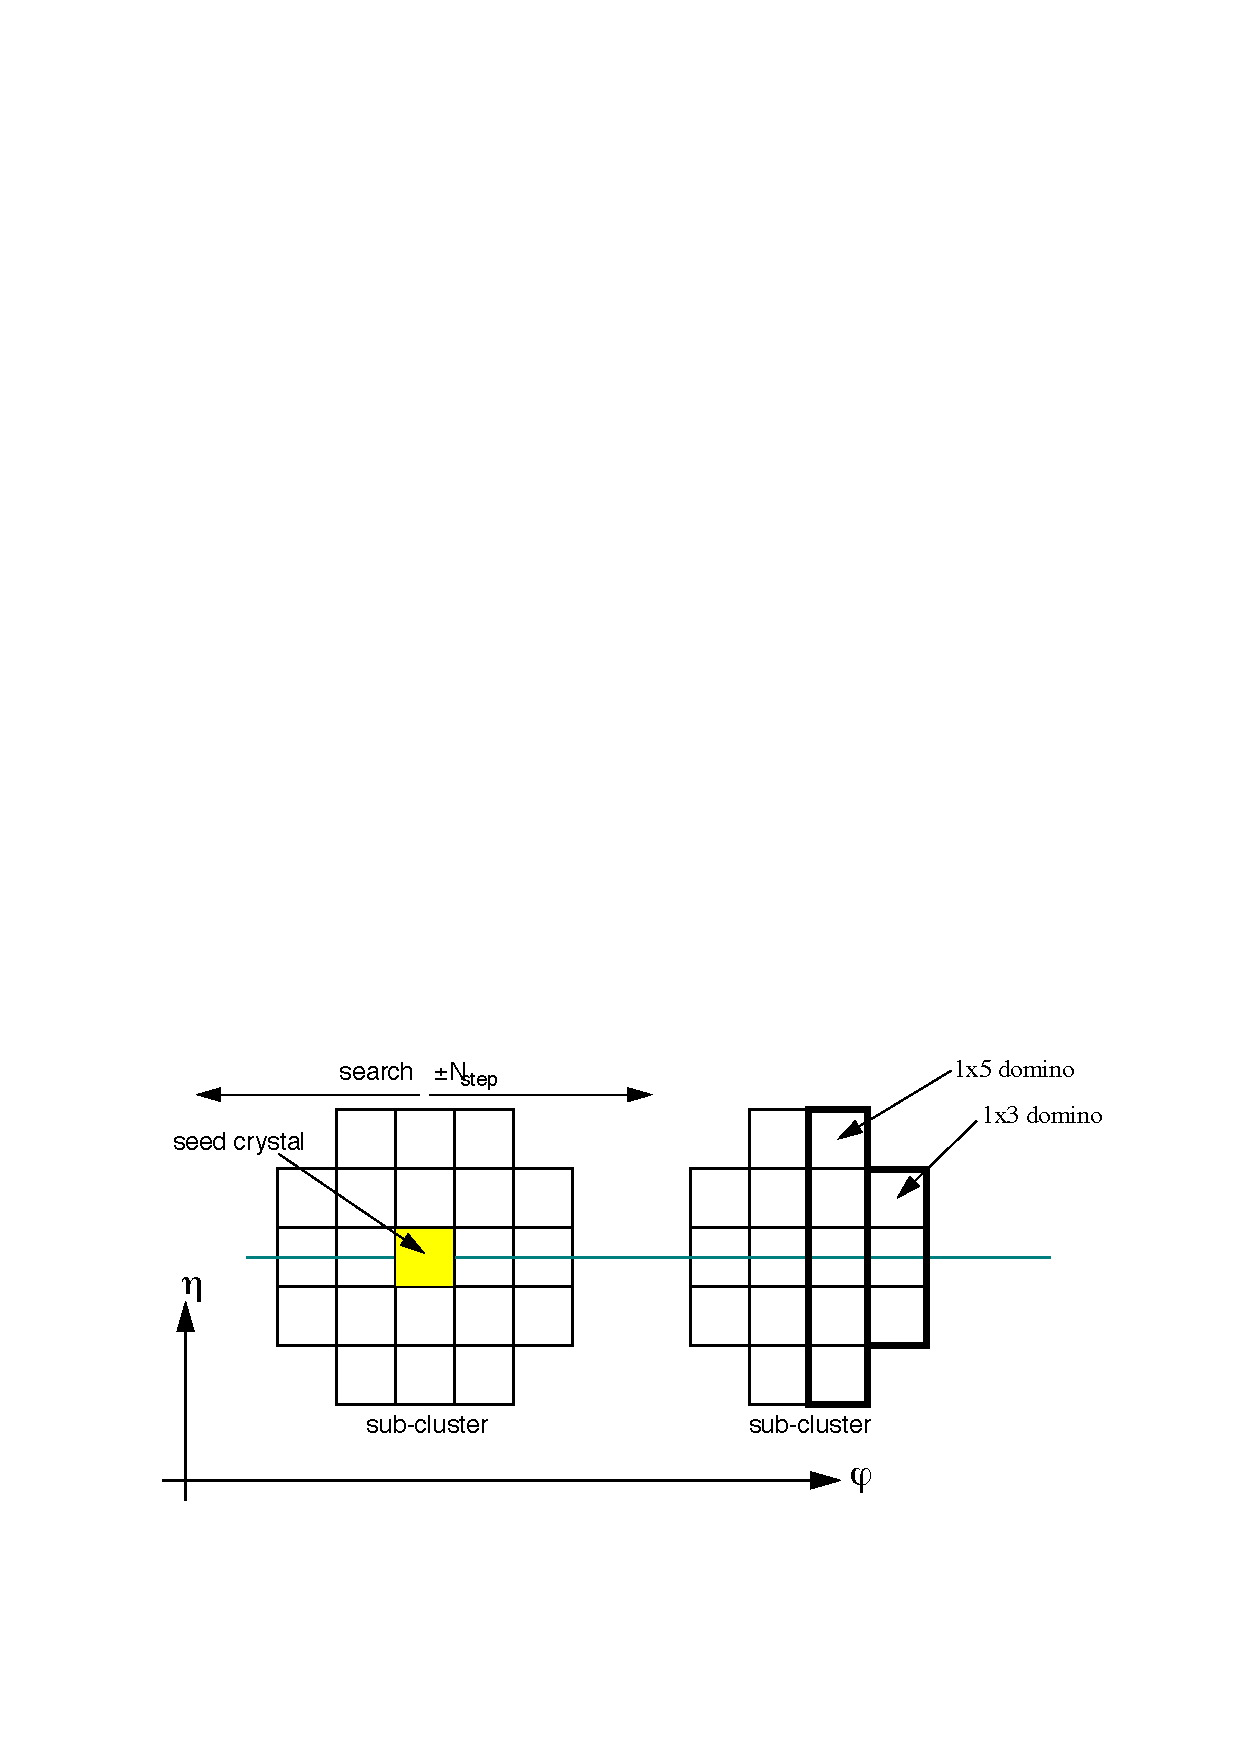
\includegraphics[width=0.8\textwidth]{cms_experiment/plots/hybrid_clustering.pdf}
  \caption[A schematic of the domino clustering algorithm]{The domino construction setup of the hybrid clustering algorithm~\cite{ecal_electron_reco}.}
  \label{fig:hybrid_algo}
\end{figure}

The final case concerns photons which reach the \ECAL without converting. These have a shower that is much more localised in \eta and \phi; about 94\% of its energy is deposited in an area of 3$\times$3 crystals and more than 97\% in an area of 5$\times$5 crystals. This provides a definition for the conversion variable, \rnine, such that, 
\begin{equation}
	R_{9} = \frac{E_{3\times3}}{E_{SC}} 
	\begin{cases}
		\text{unconverted if } R_9\geq0.94 \\
		\text{converted otherwise}.
	\end{cases}
  \label{eq:rnine}
\end{equation}
where $E_{SC}$ is the energy of the supercluster. If a photon fufills the unconverted requirement given above (Eq.~\ref{eq:rnine}) the photon energy is reconstructed as the sum of all energy deposited in the 5$\times$5 array of crystals which surround the most energetic crystal. It has been shown that using a fixed window for non-converting photons yields a better energy resolution than any clustering procedure~\cite{ecal_electron_reco}.

The location of a supercluster is determined as the energy-weighted mean position of the crystals in the supercluster. This gives a position resolution which is much smaller than the size of an individual crystal ($\sim20\times20$~mm$^{2}$). Values for an electron of $\pT=35$~GeV in the \ECAL barrel, in the absence of pileup, are $\sigma_{\eta}=1.0\times10^{-3}$, $\sigma_{\phi}=1.6$~mrad.

\subsection{Electron and photon differences}

It is clear that when only considering the \ECAL there is no difference between electrons and photons. Consequently at the level of the calorimetry there is no distinction between them, simply the idea of a supercluster which can apply to both. In the case of an electron, information from the tracker can be included using a Gaussian sum filter algorithm~\cite{tracker_electron_reco}, where a series of compatible track hits are associated to the supercluster. This is used to provide a supplementary measurement of the electrons momentum and consequently improve the energy resolution of electrons. When considering photons for an analysis an electron veto must be applied requiring that no track hits should be found close to the interaction point near the photon direction (see Chapter~\ref{chap:common_analysis_components}). An important feature of supercluster reconstruction at \CMS is that when all track information is ignored electrons and photons are identical. This is a principal ingredient in the \Hgg analysis which allows data driven calibration, validation and efficieny measurements of photons using electrons from $Z$ decays (see Sec.~\ref{sec:zee}).

% -------- PFLOW ---------
\section{Particle flow and jets}
\label{sec:pflow_jets}
A traditional approach to detector-based reconstruction is to consider the objects we measure as opposed to the underlying physics objects. These are often known as calorimeter objects, for example, a track, an electromagnetic shower or a calorimeter jet. A more modern approach is to couple information in all of the subdetector systems together to reconstruct more physical objects. For example, a charged hadron will leave a track, deposit some energy in the \ECAL and deposit the rest of its energy in the \HCAL. This technique of reconstruction is known as \PF\footnote{The offcial name inside \CMS is \GED although this is rarely used} and is particularly useful when considering jets. Whilst an electron, photon or muon have fairly characteristic signatures, hadrons often do not. The abundant number of gluons and quarks, produced in \LHC collisions, hadronise via the strong interaction as they travel away from the interaction. As they have typically high momentum the hadronistation occurs in a collimated fashion leaving a signature of several tracks and an \HCAL cluster. The \PF reconstruction algorithm can be simplistically viewed as the following procedure (more details given in Ref.~\cite{cms_pf_algo}):

\begin{enumerate}
  \item{Make small clusters from each subdetector component; tracks, \ECAL and \HCAL clusters to create a list of unassociated objects.}
  \item{Match tracks and clusters together and associate them to a newly reconstructed particle known as a \PF candidate:}
  \begin{itemize}
    \item{Tracks and clusters associated with hits in the muon chambers are tagged as \emph{muons} and removed from the list.}
    \item{Tracks and clusters associated with electrons, including bremsstrauhlung photons, are tagged as \emph{electrons} and removed from the list.}
    \item{Tracks associated to an \HCAL cluster are tagged as \emph{charged hadrons}, assigned an energy ascertained from a weighted average of the cluster energy and track momentum and subsequently removed from the list.}
    \item{Any excess cluster energy in the \HCAL is assigned as a \emph{neutral hadron} and removed from the list.}
    \item{If an \ECAL cluster is associated to an \HCAL cluster and a track, it is assigned as a \emph{charged hadron} with the appropriate weighted energy and removed from the list.}
    \item{If an \ECAL cluster is associated to an \HCAL cluster with no track, it is assigned as either a \emph{photon} or a \emph{neutral hadron} depending on the \HCAL to \ECAL energy ratio and removed from the list.}
    \item{Any remaining unlinked candidates are assigned as \emph{photons} or \emph{neutral hadrons} depending on whether they are \ECAL or \HCAL clusters.}
  \end{itemize}
  \item{In this way all information in the detector is used to create a list of candidates which can be any of a muon, electron, photon, charged hadron or neutral hadron.}
  \item{These are then used to construct composite detector objects such as jets if necessary.}
\end{enumerate}

Particle flow jets are constructed using the anti-$k_{T}$ algorithm~\cite{anti_kt_algo}. This algorithm is both infrared and collinear (IRC) safe and preferentially clusters soft (low \pT) jets with hard (high \pT) jets to be robust in the \LHC pileup conditions. These jets can then be additionally tagged as $b$ or $c$ (i.e.~those containing a bottom or charm quark respectively) using techniques of the type described in~\cite{b_tag}. There are also energy corrections applied to jets to account for pileup ($\rho$ subtraction technique as described in section~\ref{sec:pileup}), non-uniform detector response (\pT and \eta dependent corrections derived from \MC simulation) and data-MC differences (residual \pT and \eta corrections derived from $\gamma+$jet and $Z+$jet samples in data), see Ref.~\cite{jet_e_corrs} for details. The clustering, and subsequent energy correction, of jets in this way also provides a measure of the missing transverse energy (\MET), the amount of energy in an event taken away by undetectable particles such as neutrinos. A comparison of the jet energy resolution, as a function of jet \pT, for calorimeter jets and particle flow jets is shown in Fig.~\ref{fig:muon_jet_res} for simulated data at $\sqrt{s}=7$~TeV.

A \PF photon is quite different to the photons used in the analysis, whose reconstruction is decribed above in Sec.~\ref{sec:photon_reco}. \PF is useful for tagging physics objects like tau's or b's and for isolation sums (see following Sec.~\ref{sec:iso}) but is not necessarily the best for reconstructing well measured objects like photons, electrons and muons.

\begin{figure}
  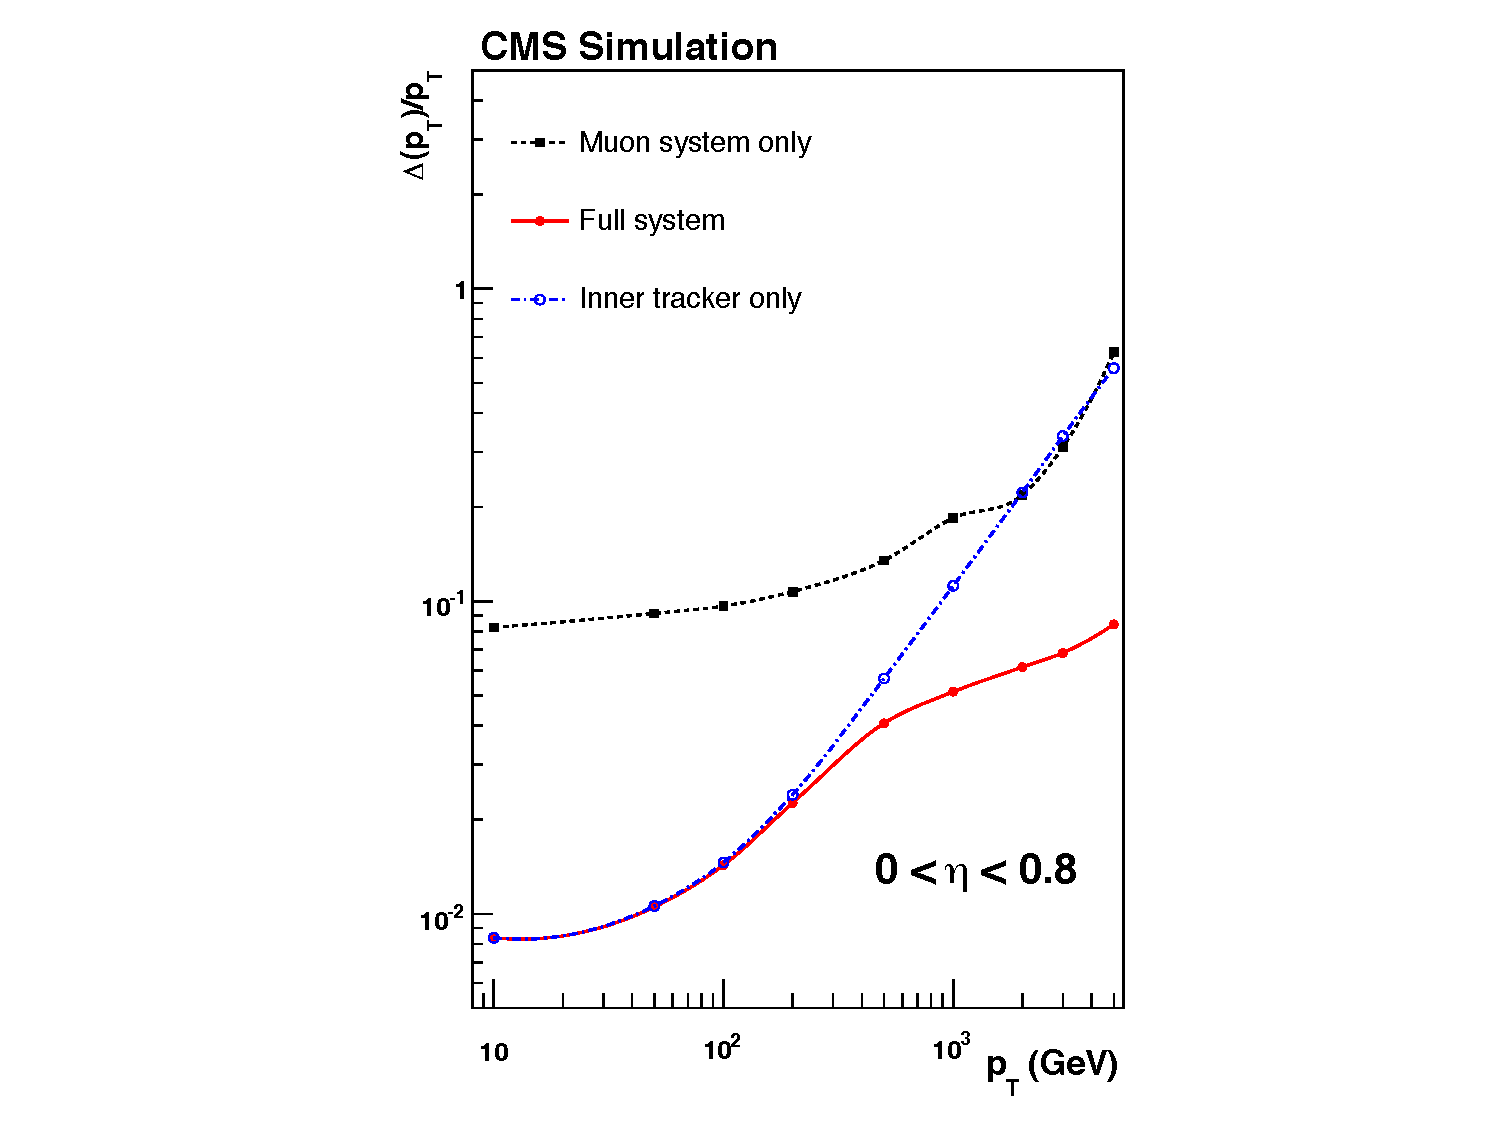
\includegraphics[height=0.4\textwidth]{cms_experiment/plots/MuonResolution_fix.pdf}
  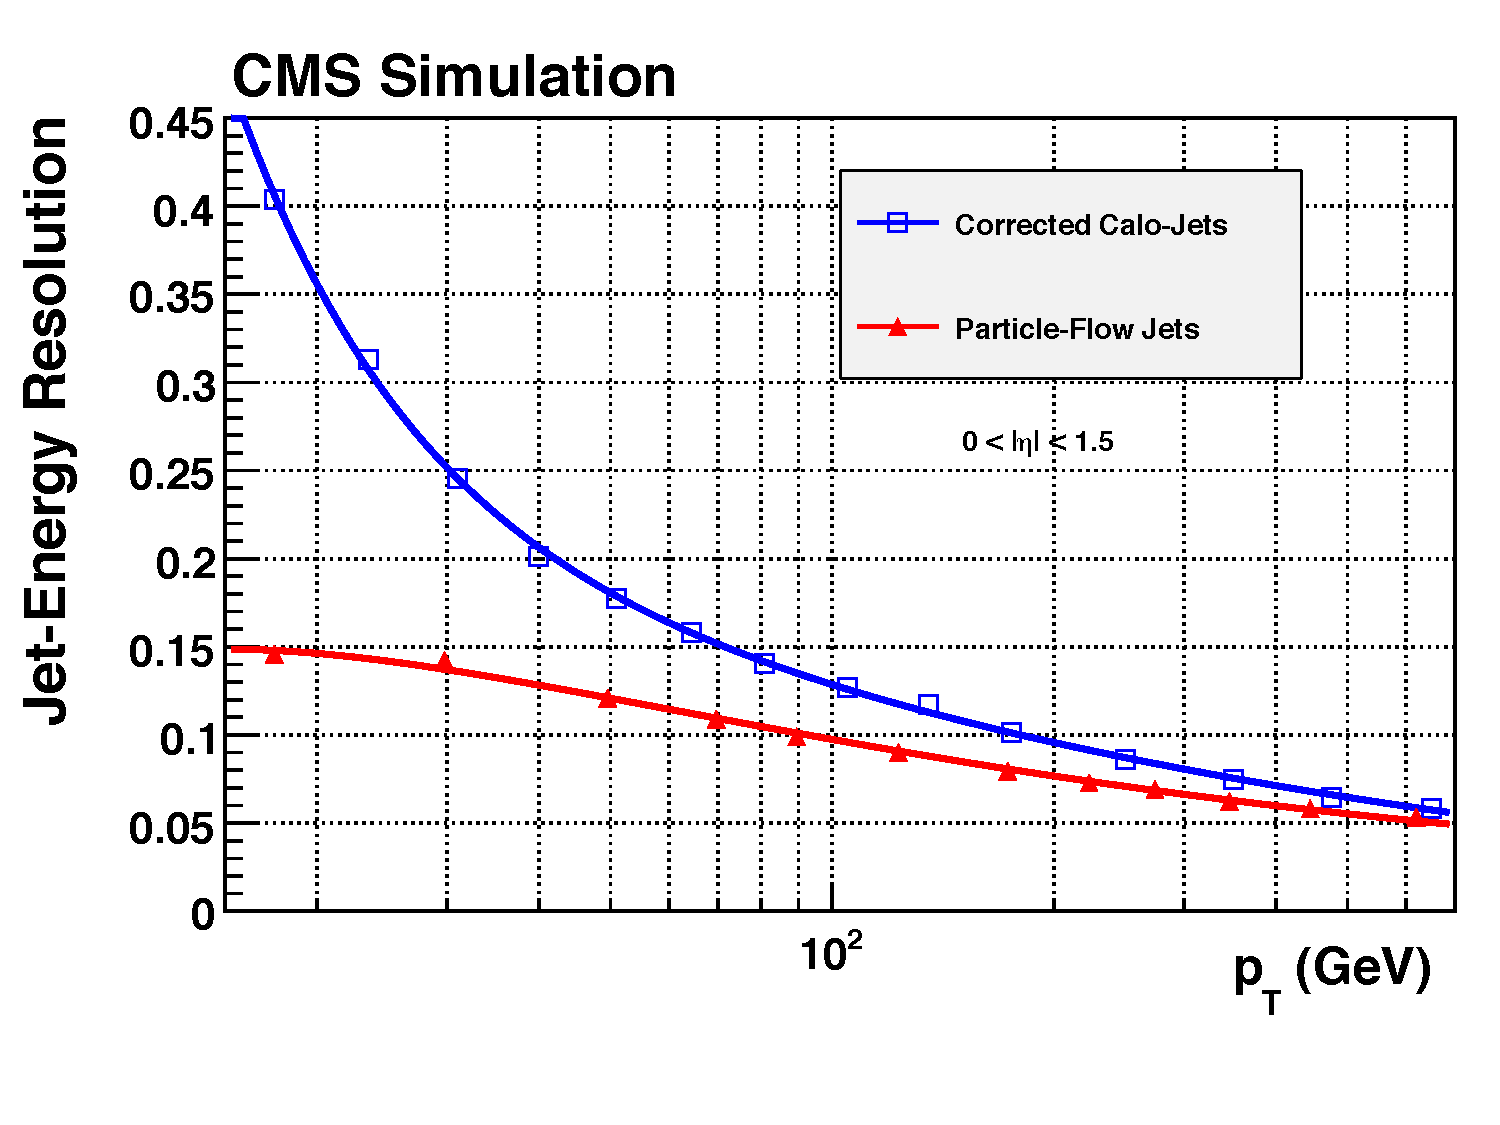
\includegraphics[height=0.4\textwidth]{cms_experiment/plots/BarrelResolutionPFAndCalo_fix.pdf}
  \caption[Particle flow jet resolution]{\textbf{Left:} The muon \pT resolution, in \MC simulation, as a function of \pT for muons in the range $0<|\eta|<0.8$ when using only the muon system (black), only the tracking system (blue) and using both (red)~\cite{CMS_JINST}. \\ \textbf{Right:} The jet energy resolution, in \MC simulation, as a function of jet \pT when using \PF jets as compared to calo jets~\cite{cms_pf_performance}.}
  \label{fig:muon_jet_res}
\end{figure}

\section{Isolation}
\label{sec:iso}

One way of differentiating between real (prompt) photons from Higgs decays and fakes is the use of isolation. One would expect that in the absence of pileup a photon from a Higgs is not in a jet and therefore would be isolated, which is to say there are no other particles (detector activity) in its vicinity. For a jet faking a photon (which is nearly always a \pizero) this is not the case and one would expect the \pizero to be surrounded by additional hadronised particles (detector activity in the tracker, \ECAL and \HCAL). In the \CMS \Hgg analysis isolation sums are used to distinguish prompt photons from fakes. Three variables are used which consider the isolation of each photon relative to activity in the surrounding environment. The procedure is to create a hollow cone around the photon candidate (of outer radius $\Delta R_{O}$ and inner radius $\Delta R_{I}$, where $\Delta R = \sqrt{\Delta\eta^{2}+\Delta\phi^{2}}$) and sum the energy contained in that cone of \PF candidates; charged hadrons, neutral hadrons and electrons/photons. These three variables are defined in the following way:

\begin{itemize}
  \item{\textbf{Charged hadron isolation:} Sum of charged hadron \PF candidates \ET in cone of $\Delta R_{O}=0.3$ and $\Delta R_{I}=0.02$.} 
  \item{\textbf{Neutral hadron isolation:} Sum of neutral hadron \PF candidates \ET in cone of $\Delta R_{O}=0.3$ and $\Delta R_{I}=0.0$.}
  \item{\textbf{$e/\gamma$ isolation:} Sum of $e/\gamma$ \PF candidates \ET in cone of $\Delta R_{O}=0.3$ with a central \eta strip of 0.070 (0.015) removed for barrel (endcap) photons.}
\end{itemize}

\section{Pileup}
\label{sec:pileup}

There can be up to $1.1\times10^{11}$ protons in each bunch at the \LHC which results in multiple interactions (which can be as many as 50 primary vertices) per bunch crossing. This effect is known as pileup and can present a challenge when finding the primary vertex. This effect produces additional energy in each event which originates from somewhere other than the primary vertex. To combat the latter of these two effects a technique called $\rho$ subtraction is used to correct the energy of jets and isolation sums for pileup. $\rho$ is defined as a per event quantity and is computed by summing the energy in all the calorimeters and dividing by the calorimeter area and thus represents the average energy density in the detector per event. The quantity \rho can then be used to subtract energy from isolation sums or alternatively its correlation with isolation sums in background samples can be exploited by multivariate analysis techniques.





  \chapter{Common analysis components}
\label{chap:common_analysis_components}

This thesis describes three complementary analyses in the Higgs to two photons search at CMS. These differ in their photon selection, event selection, event classification (or categorisation) and statistical methods for extracting results. They are described in the following chapter (Chapter~\ref{chap:selection_and_categorisation}). However, there are many components which they share. These are detailed below.

As we have seen in Eq.~\ref{eq:invmass} and~\ref{eq:dipho_inv_mass}, repeated below in Eq.~\ref{eq:invmass2} for convenience, the diphoton invariant mass is constructed from the two photon energies and the angle between them. 
\begin{equation}
  m_{\gamma\gamma} = \sqrt{2E_{1}E_{2}(1-\cos\alpha)}
  \label{eq:invmass2}
\end{equation}
Consequently, important considerations for this analysis are photon energy resolution and good opening angle resolution. The latter is completely dominated by the vertex resolution, as the position resolution of the photons (the location at which they hit the \ECAL) is negligible in comparison. Details of how this is exploited in the analyses are given at the end of this chapter in Sections~\ref{sec:photon_energy} and~\ref{sec:vtx_reco}. The selection of events is described in the chapter after this (Chapter~\ref{chap:selection_and_categorisation}) alongside the categorisation, or binning, scheme whereby events which share similar signal to background ratios are collected into different classes of event, which take advantage of areas of phase space which share similar signal to background ratios.
After a preliminary discussion of multivariate analysis techniques, the datasets, the triggering and the \MC simulation are discussed.

\section{Boosted Decision Trees}
\label{sec:bdts}
Multivariate analyses (\acs{MVA}) are commonly used in High Energy Physics analyses to extract the maximum possible signal sensitivity in cases where the background rates are high. The advantage of \MVAs is that given a set of input variables a selection scheme can be built, to classify or correct events, in a multidimensional phase space to exploit differences between the signal and background in these variables and importantly in the correlations between them. A particular type of \MVA which is used widely in this analysis is the \BDT. \BDTs are preferred because they are more robust to the inclusion of variables which have little or no discriminating power. There are two broad types of \BDT used, one is known as a regression \BDT and the other as a classification \BDT~\cite{bdt,bdt2,bdt3}. 

\subsection{Classification \acs{BDT}}
A classification \BDT will, given a set of input variables, assign a value (typically between $-1$ and $1$) to each event based on how signal-like that event is. This serves to collapse all the event information into one discriminating variable which can be used to classify differences between the signal and background. The input is provided as the probability distributions (which can be supplied as binned or unbinned data samples or as a functional form) of the background and signal for a set of ``input variables". The process involves construction of a series of \aclp{DT} (\acs{DT}) complemented by a ``boosting" step which serves to mitigate against ``overtraining" on fluctuations within the training samples. This analysis chooses a particular type of decision tree boosting known as ``gradient" boosting because it is more robust against outliers or mislabelled data points~\cite{TMVA}.

The \DT is built by applying sequential cuts to the input variables and assessing the relative signal purity, $p$, in the sub-sample remaining after each cut
\begin{equation}
  p = \frac{N_{s}}{N_{s}+N_{b}},
\end{equation}
where $N_{s}$ and $N_{b}$ are the sum of weights of the signal and background remaining in each sub-sample. A threshold criterion, known as the Gini index~\cite{TMVA} $p(1-p)$, is applied to decide whether to split the sample further. The process continues and the splitting is curtailed when either the threshold or the user defined maximum tree depth (number of subsamples allowed) is reached. The value of each cut is varied such that the signal purity, $p$, in each sub-sample is maximised. An event is assigned a value of $-1$ or $+1$ depending on whether it falls into a sub-sample with $p>$0.5 or not. Clearly some fraction of events will be misclassified where the actual number which get misclassified will depend on the discriminatory power available from the chosen input variables. In order to reduce this effect a series of \DTs are trained and each assigned a weight derived by the ``boosting" process. 

We assign each \DT as a member of a family of $M$ functions, $f(\vec{x};\vec{a}_{m})$, which depend on the input variables, $\vec{x}$, and the set of cuts in that tree, $\vec{a}_{m}$. The object is to construct an overall decision tree which consists of the weighted average of each \DT,
\begin{equation}
  F(\vec{x};\vec{\beta},\vec{a}) = \sum_{m=0}^{M} \beta_{m}f(\vec{x},\vec{a}_{m}) \;\;\;\;\; \textrm{where} \;\; \vec{\beta} = (\beta_{0},\beta_{1}...\beta_{M}).
\end{equation}
For the ``adaptive" boost algorithm the input events for training the proceeding tree are reweighted by the fraction that get misclassified in the previous tree. I.e.~the background events get reweighted by the total fraction of background events which were classified as signal in the previous tree and the signal events get reweighted by the total fraction of signal events which were classified as background in the previous tree. In the ``gradient" boosting procedure, which constitute the majority of \BDTs used in this thesis, the weight for sucessive trees is obtained by minimising the deviation in the loss function (Eq.~\ref{eq:bdt_loss_fcn}) each time a new tree is added\footnote{ Friedman showed that for certain choices of loss function the ``gradient" boost and ``adaptive" boost procedures are identical, although this is not the case for a general loss function, nor the loss function of the form used in this thesis, shown in Eq.~\ref{eq:bdt_loss_fcn}~\cite{bdt3}.}. The loss function, between the weighted tree response $F(\vec{x};\vec{\beta},\vec{a})$ and the true output $y$ obtained from the training sample, in this case is
\begin{equation}
  L(F,y) = \ln(1+e^{-2F(\vec{x})y}).
  \label{eq:bdt_loss_fcn}
\end{equation}
A common procedure when constructing a \BDT to check for overtraining is to split both the background and signal into two independent samples. One is used to \emph{train} the \BDT and one is used to \emph{test} the response of the output. Clearly one requires that both the training and independent test sample look the same in the output variable. This is usually quantified by use of a Kolmogorov-Smirnov test, which broadly speaking ascertains the probability that the training and test samples originate from the same underlying distribution~\cite{kol_smir}. 

In this way the output of $F(\vec{x};\vec{\beta},\vec{a})$ for a classification \BDT will be a ``semi-continuous" output\footnote{ In the sense that each decision tree will give a discrete output of either signal-like or background-like such that the boosted output of the numerous trees in the forest contains several hundred (depending on the number of trees) discrete values in the range $[-1,1]$.} from $-1$ to $+1$ with signal events in general given a higher score than background events.

\subsection{Regression \acs{BDT}}
A regression \BDT is used to estimate the true value of some variable given the values and correlations of several other variables. They are commonly used for correcting the energy of a particular object, for example a photon. Given a \MC source of photons the ``true" energy is regressed from the position, shape and raw energy of the supercluster. For regression \BDTs the output $F(\vec{x};\vec{\beta},\vec{a})$ represents the estimated corrected energy and the boosting procedure targets minimising the deviation between this and the true energy in \MC events. 

\section{Data samples and triggering}

The data consists of two independent samples of proton-proton collisions collected by the CMS experiment at the \LHC in 2011 and 2012 with a centre-of-mass energy, $\sqrt{s}$, of 7 and 8 TeV, respectively. The total integrated luminosity of the two samples is 5.1~\fb and 19.7~\fb in 2011 and 2012, respectively, and they are collectively referred to as \LHC Run 1. The response of the detector has changed considerably over this period and much of the variation is modelled by the \MC simulation. Figure~\ref{fig:intlumi} shows the integrated luminosity delivered to and recorded by \CMS during \LHC Run 1.

\begin{figure}
  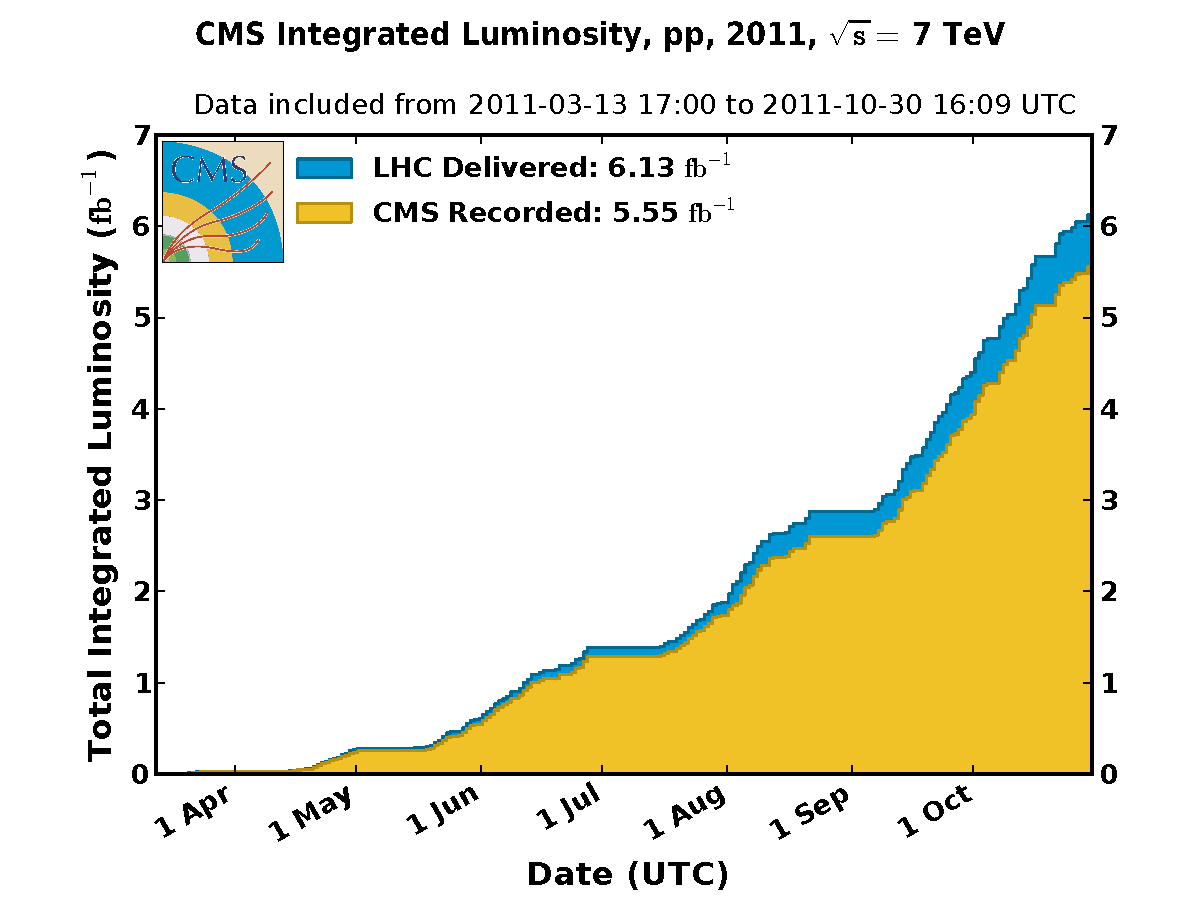
\includegraphics[width=0.49\textwidth]{analysis_comps/plots/int_lumi_2011.pdf}
  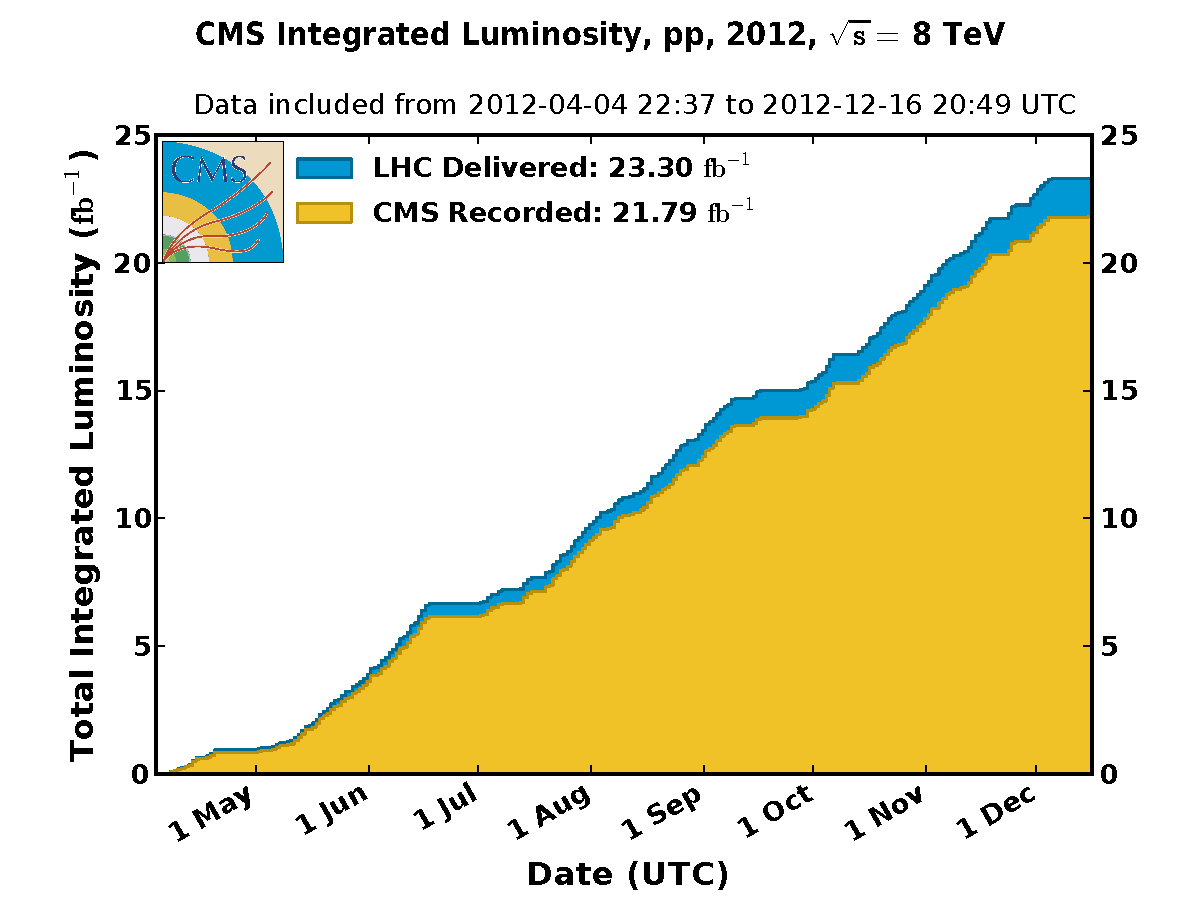
\includegraphics[width=0.49\textwidth]{analysis_comps/plots/int_lumi_2012.pdf}
  \caption[The total integrated luminosity delivered to and recorded by \acs{CMS} during the 2011 and 2012 run periods]{The total integrated luminosity delivered to and recorded by CMS during the 2011 (left) and 2012 (right) run periods. Due to down time of various subsystems in \CMS during run periods, particularly the \ECAL, the recorded luminosity given here is not exactly equivalent to the integrated luminosity of the datasets used in the analysis~\cite{lumi1,lumi2}.}
  \label{fig:intlumi}
\end{figure}

Events are selected for the analysis by requiring they pass an asymmetric diphoton trigger with \ET thresholds of 26 (18) and 36 (22) GeV for the leading (trailing) photon in the 2011 and 2012 runs, respectively. The candidates are also required to have either a high value of \rnine or to pass a loose calorimetric identification and isolation requirement. High trigger efficiency is achieved by selecting photon candidates which pass either requirement. The efficiency of the trigger for the analysis preselection is 99.5\%.

\subsection{Monte Carlo Simulation}
\label{sec:mc}

Accurate simulation of detector effects and efficiency is highly important. Knowledge of the expected Higgs signal shape is clearly essential and although the size and shape of the \mgg background is entirely data driven when extracting results, simulating the kinematics, shower shape and resolution properties of the background is important when training the selection and optimising the categorisation of events. 

As explained in Chapter~\ref{chap:theory} the two main production mechanisms for a \SM Higgs boson at the \LHC are \ggH and \VBF. Typically the latter is produced at much higher Higgs \pT and this feature is exploited in the analysis (see Fig.~\ref{fig:gen_level}). Consequently, it is important to model the \pT distribution of these two production modes accurately. The signal samples for these two processes are generated using \POWHEG~\cite{powheg1,powheg2} at NLO interfaced with \PYTHIA~\cite{pythia} including a reweighting factor which matches their \pT spectrum to that when including the NNLO and NNLL terms. For the associated production modes, with a $W^{\pm}$, $Z$ or $t$ quarks, (\VH and \ttH) only \PYTHIA is used. The \SM Higgs boson cross sections and branching fractions, and their uncertainties, are taken from Ref.~\cite{LHCHiggsCrossSectionWorkingGroup3}

The spin-2 graviton with minimal couplings, \graviton, has two production mechanisms, one via gluon-fusion ($ggX$) and one via quark-antiquark annihilation ($q\bar{q}X$). The graviton samples are generated using the \JHU generator~\cite{jhu}. In these samples the signal events are reweighted such that the graviton \pT spectrum matches the Higgs \pT spectrum in the \SM signal samples. The kinematic properties of a spin 2 \textit{graviton-like} Higgs are not well defined and can depend on the specifics of the model in question. Matching the \pT spectrum of the spin-2 samples with the \SM spin-0 ensures that no discrimination arising from model dependence of the \pT distribution will arise. 

The simulated background samples are used solely for cut and category optimisations and training of multivariate discriminants. The background which contains the \QCD continuum of prompt photons (referring back to Chapter~\ref{chap:theory} these are produced by Born and box diagrams) is simulated using \SHERPA~\cite{sherpa} at 8~\TeV and \MADGRAPH~\cite{madgraph} at 7~\TeV. The prompt-fake and fake-fake backgrounds, in which one or both photons are faked by a neutral meson (usually a \pizero) reconstructed as a photon, are generated using \PYTHIA. Samples of \Zee, \Zmumu and \Zmumugamma used for data/MC comparisons are generated with \POWHEG.

All of these \emph{generator level} samples are then run through the full \CMS detector simulation using \GEANT~\cite{geant}. This includes the effect of overlapping vertices (pileup) and detector effects (such as noise and crystal degradation) in four time periods; Run2011 (5.1~\fb), Run2012AB (5.3~\fb), Run2012C (7.1~\fb) and Run 2012D (7.3~\fb).


\subsection{Pileup and beamspot reweighting}
\label{sec:pileup_beamspot}

An important difference between the simulated samples and the data which can have a large impact on the analysis is the distribution of the number of primary vertices. The \emph{pileup} in the event affects many important analysis variables, for example photon shower shape and photon isolation as well as the diphoton invariant mass if the chosen vertex is wrong. Consequently the \MC events are reweighted such that the pileup distribution matches that in data. The reweighting technique is validated using \Zmumu events as shown in Fig.~\ref{fig:pileup} for the 7 and 8~\TeV samples. 

\begin{figure}
  \begin{center}
  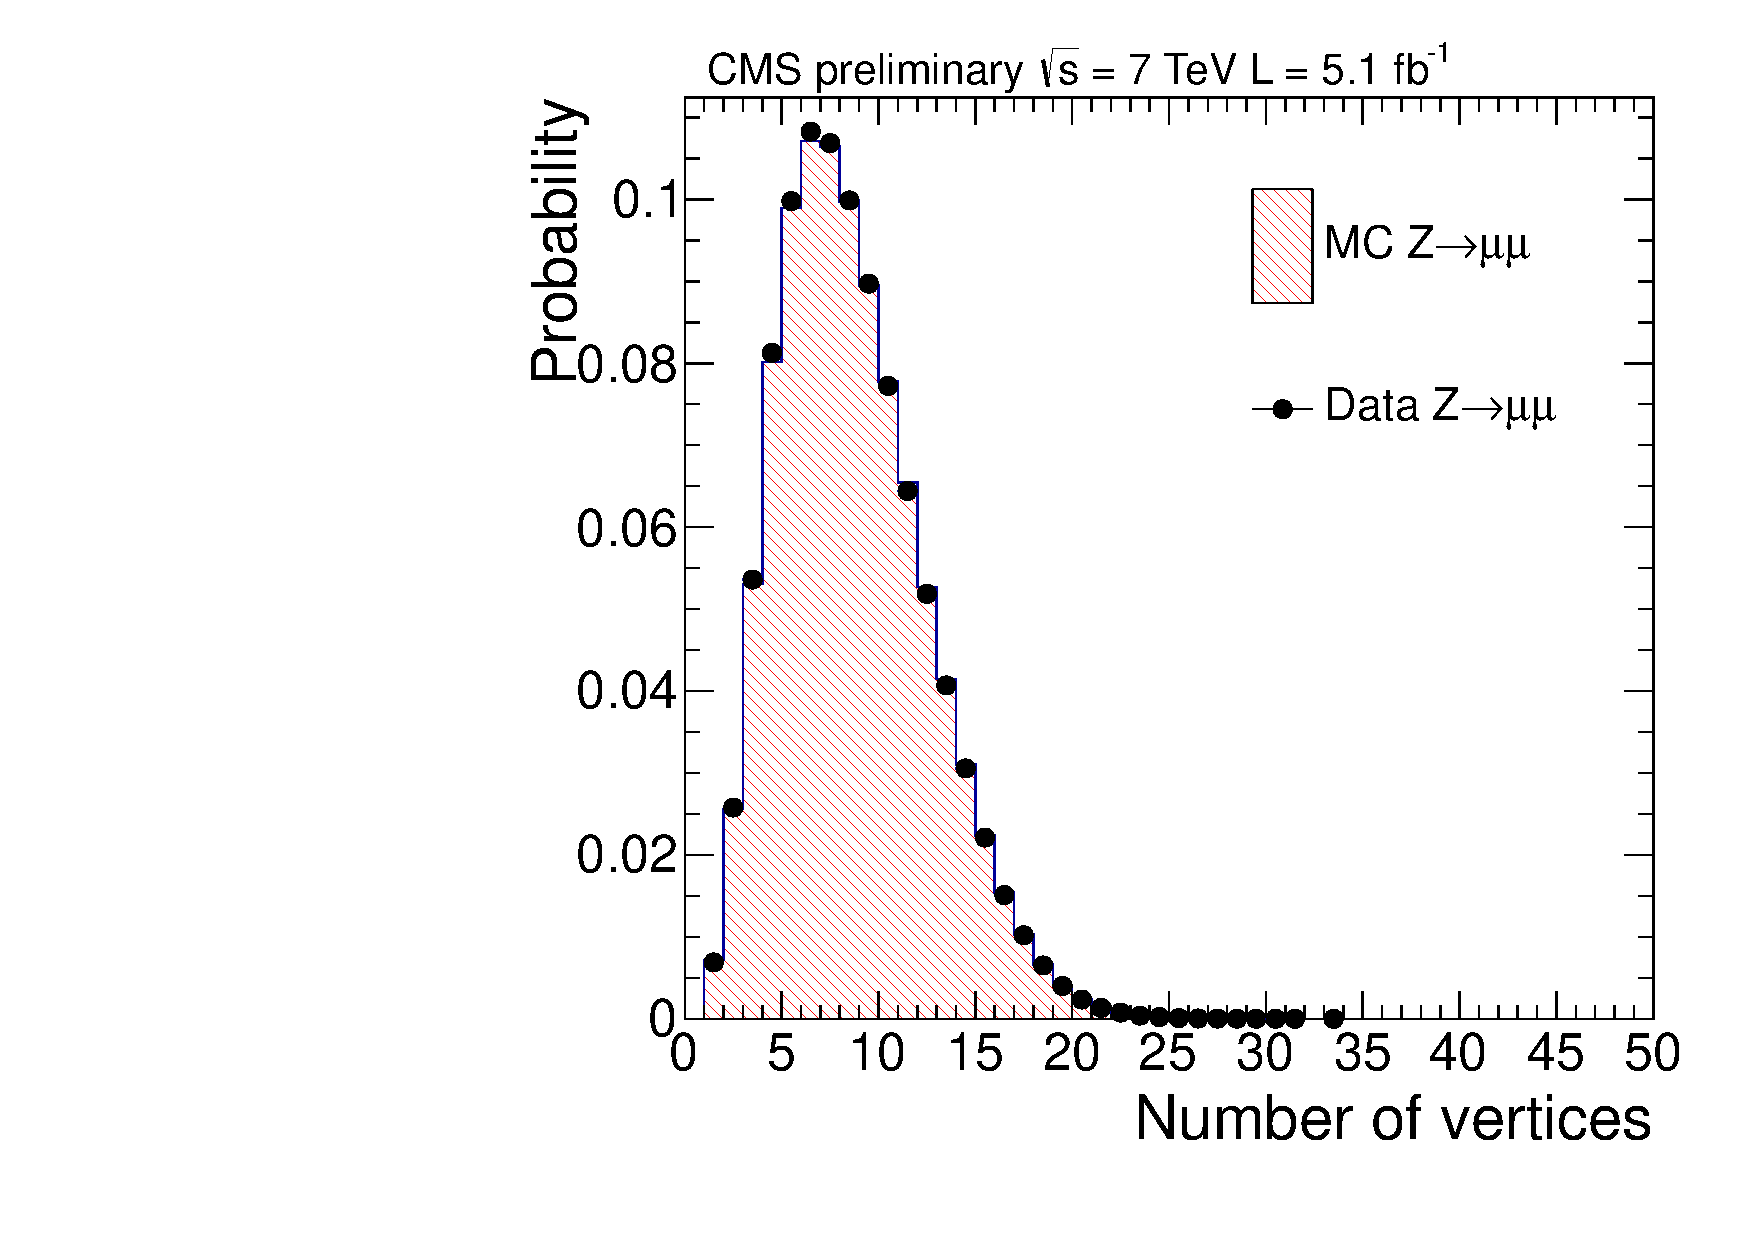
\includegraphics[width=0.49\textwidth]{analysis_comps/plots/nvtx_zmumu_2011.pdf}
  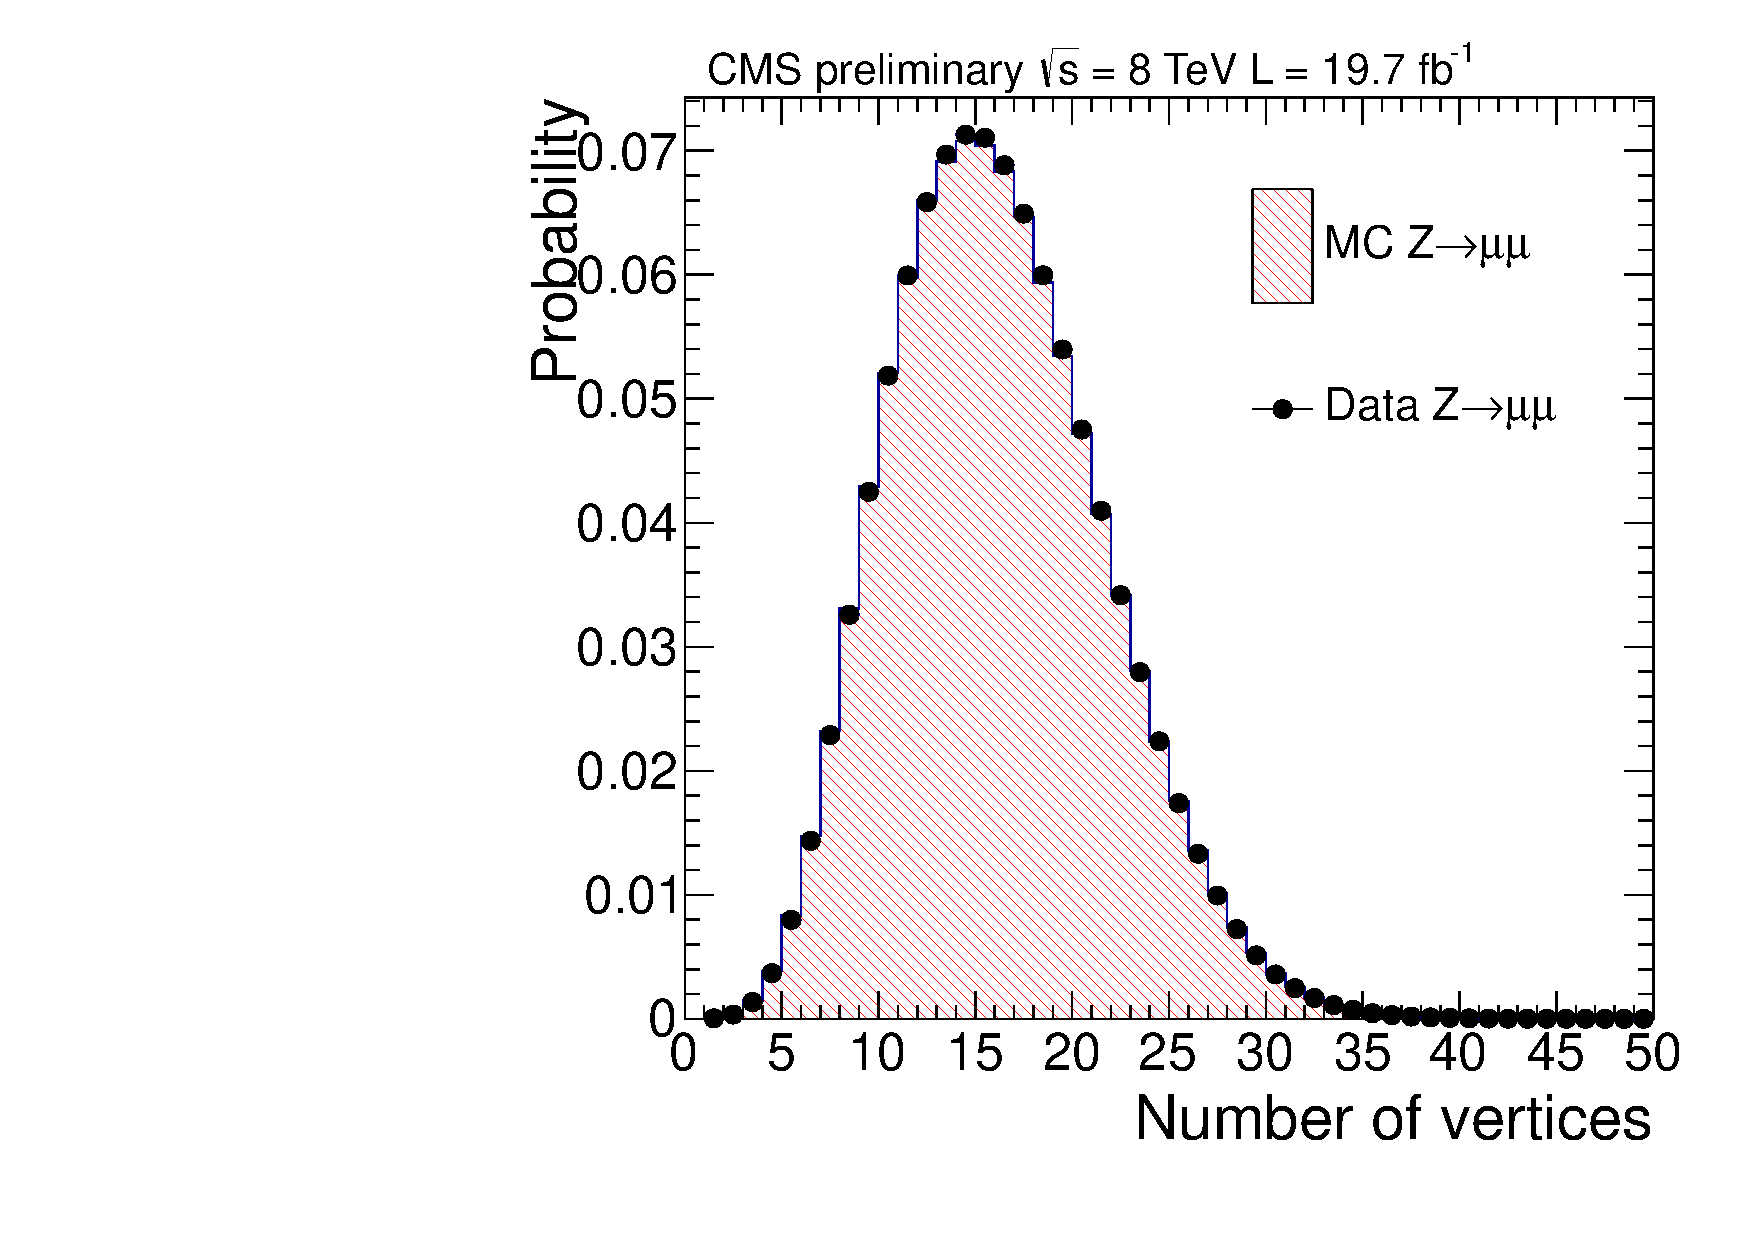
\includegraphics[width=0.49\textwidth]{analysis_comps/plots/nvtx_zmumu_2012.pdf}
  \caption[Distribution of the number of reconstructed vertices]{Distribution of the number of reconstructed vertices in the 2011 (left) and 2012 (right) run periods. Calculated using the Deterministic Annealing algorithm in~\cite{deterministic_annealing} for \Zmumu events in data (black dots) and MC events (red histogram) after reweighting.}
  \label{fig:pileup}
  \end{center}
\end{figure}

When the chosen vertex is incorrect the mass resolution is dominated by the spread in position of the pileup vertices (known as the beamspot width, $\sigma_{z}^{beamspot}$). Accurate modelling of this spread is important so that the resolution of wrong vertex events in simulation matches that in data. The \MC sample overestimates the beamspot spread by some 20\% so a simple reweighting is implemented for \MC events in which the wrong vertex is chosen (as the effect is negligible for events in which the chosen vertex is correct) such that the distribution of the distance between the chosen vertex position and the true vertex position, $\delta z=z_{chosen}-z_{true}$, match between data and \MC. The effect with and without reweighting compared to data is shown in Fig.~\ref{fig:beamspot}.

\begin{figure}
  \begin{center}
  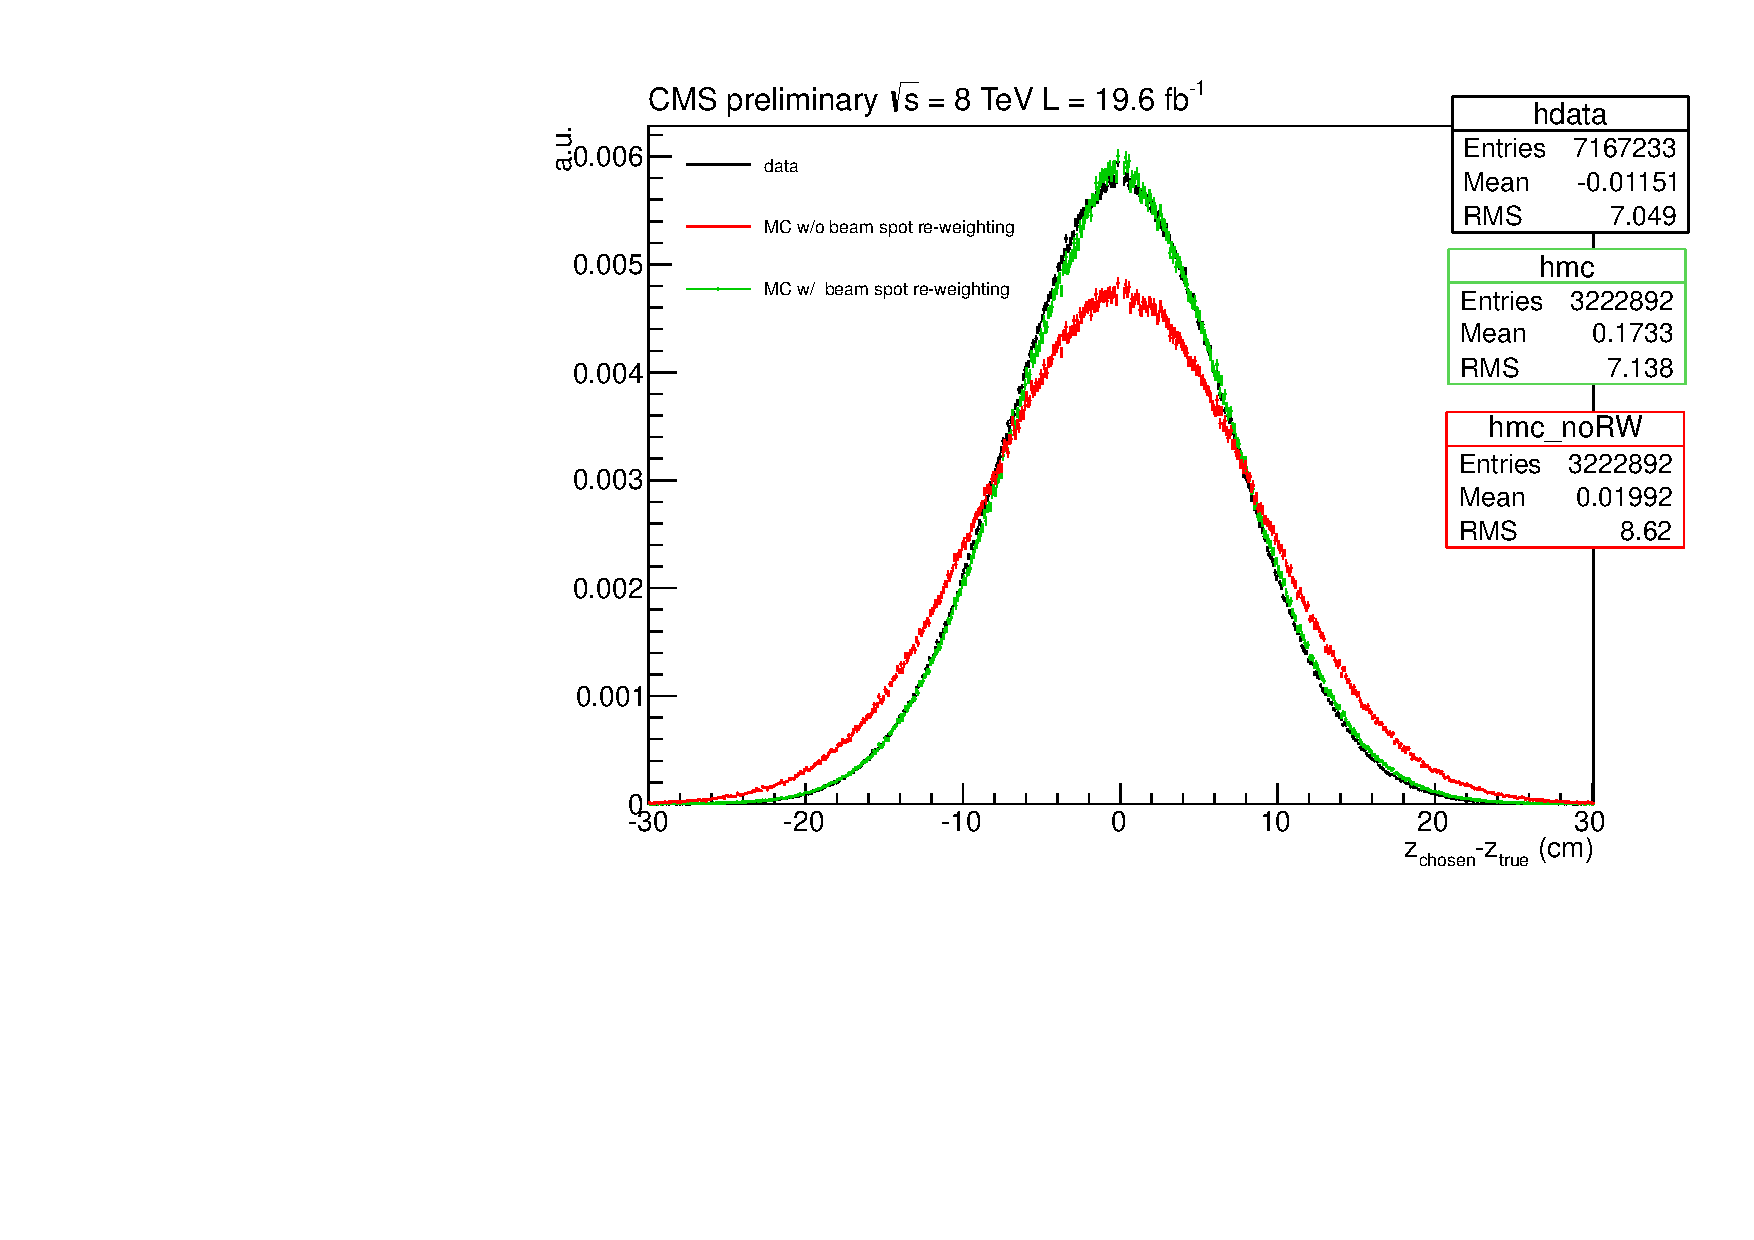
\includegraphics[width=0.55\textwidth]{analysis_comps/plots/beamspot.pdf}
  \caption[Distribution of $\Delta z$ (the distance between the chosen vertex and the true vertex in the $z$ direction)]{Distribution of $\Delta z$ (the distance between the chosen vertex and the true vertex in the $z$ direction) for data (black), the \MC simulation (red) and the \MC simulation after beam spot reweighting (green) for \Zmumu events.}
  \label{fig:beamspot}
  \end{center}
\end{figure}

\section{Energy measurement of photons}
\label{sec:photon_energy}

The photon energy obtained from the supercluster sum described in Section~\ref{sec:ecal}, even when including the intercalibration and transparency corrections shown in Fig.~\ref{fig:ecal_laser_corrs}, does not give the most optimal resolution for the energy measurement of photons at \CMS. On top of this energy (known as the \emph{raw} supercluster energy, $E_{raw}$) it is also valuable to correct for additional energy losses. These arise from bremsstrahlung; where the photon converts in the material upstream of the \ECAL and the two electrons radiate additional photons and thus some of the photon shower is missed, and from local non-containment of the shower; where some energy is lost due to small gaps between \ECAL crystals and larger gaps between ``modules" or sections of crystals. These corrections are obtained using a specialised regression \BDT (see Sec.~\ref{sec:bdts}) trained on a \MC source of prompt photons from a sample containing photons and jets. The \BDT targets accurate measurements of individual photons' energies by correcting the raw supercluster energy and provides an estimate for the energy resolution of each photon given the position and shower shape of the supercluster. The training is done separately for barrel and endcap photons (as the cluster shapes look very different for these two distinct regions) and is also performed separately for the 7 and 8 TeV datasets. The following input variables are used:
\begin{itemize}
  \item the global position of the supercluster in \eta and \phi;
  \item a collection of shower shape variables which aim at providing information on the likelihood and location of a photon conversion and the degree of showering in the material:
  \begin{itemize}
    \item the \rnine of the supercluster (as previously described in Section~\ref{sec:ecal});
    \item the ratio of the 5$\times$5 crystal energy to the raw supercluster energy (equivalent to $R_{25}$);
    \item the energy weighted \eta-width and \phi-width of the supercluster (in other words the spread of the shower);
    \item the number of basic clusters in the supercluster;
    \item the ratio of energy in the \HCAL behind the supercluster to the \ECAL energy of the supercluster, $H/E$;
    \item the ratio of the preshower energy to the raw supercluster energy (endcap only).
  \end{itemize}
  \item a collection of the seed crystal and the seed cluster variables which aim at providing information about energy lost through gaps and cracks between crystal and crystal modules:
  \begin{itemize}
    \item the relative energy and position of the seed cluster;
    \item the local energy covariance matrix;
    \item energy ratios between the seed and the 3$\times$3 and 5$\times$5 areas around the seed;
    \item the \eta and \phi index of the seed crystal and the position of the seed cluster relative to the crystal centre. 
  \end{itemize}
  \item additionally, the number of primary vertices and the median energy density, \rho, (see Sec.~\ref{sec:pileup}) are included to account for residual energy scale effects from pileup.
\end{itemize}
The regression is trained using an additional feature to that described in Sec.~\ref{sec:bdts} whereby the target is to predict the full probability distribution of the ratio of the true energy to the raw energy, $E_{true}/E_{raw}$. The target is a double Crystal Ball~\cite{CrystalBallShape} distribution which consists of a Gaussian core and power law tails on either side. This can be fully parametrised by six variables, the Gaussian mean and width ($\mu$, $\sigma$), the power parameters ($n_{L}$, $n_{R}$) and the power law tail cutoff parameters ($\alpha_{L}$, $\alpha_{R}$). Each of these parameters has a non-parametric dependence on the input variables, $\vec{x}$, and this is \emph{learned} by the regression training whilst simultaneously minimising the likelihood,
\begin{equation}
  -\ln \mathcal{L} = - \sum_{MC \; photons} \ln p\bigl[E_{true}/E_{raw} | \mu(\vec{x}),\sigma(\vec{x}),\alpha_{L}(\vec{x}),\alpha_{R}(\vec{x}),n_{L}(\vec{x}),n_{R}(\vec{x})\bigr],
\end{equation}
for the double Crystal Ball distribution, $p$. The most probable value for the true energy estimate of each photon is then given by,
\begin{equation}
  E(\vec{x},E_{raw}) = \mu(\vec{x})E_{raw}
\end{equation}
and the per-photon energy resolution is given by, 
\begin{equation}
  \frac{\sigma_{E}(\vec{x},E_{raw})}{E(\vec{x},E_{raw})} = \frac{\sigma(\vec{x})}{\mu(\vec{x})}.
\end{equation}
In this way the regression predicts the full probability distribution of $E_{true}/E_{raw}$ per photon given a particular configuration of the input variables, $\vec{x}$, and provides an estimate of the optimal energy correction and the energy resolution per photon. A comparison of this distribution with a statistically independent \MC sample is shown for the 8~\TeV training in Fig.~\ref{fig:regression_training}. 

\begin{figure}
  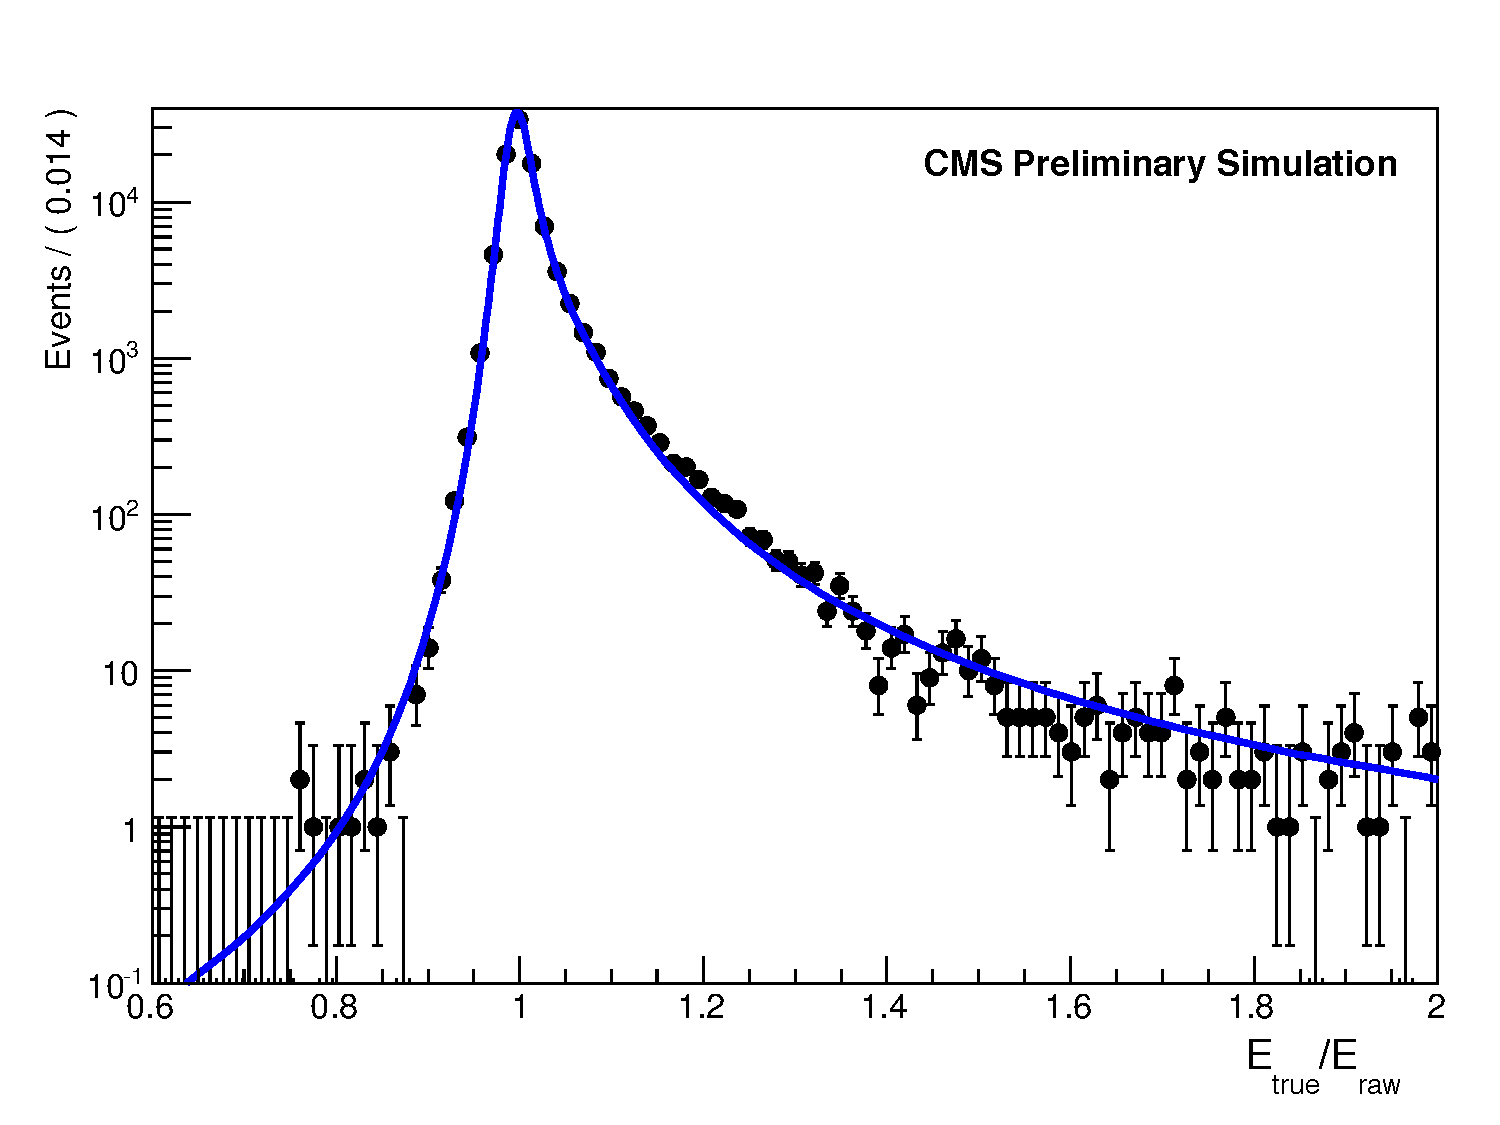
\includegraphics[width=0.48\textwidth]{analysis_comps/plots/regression_barrel_fix.pdf}
  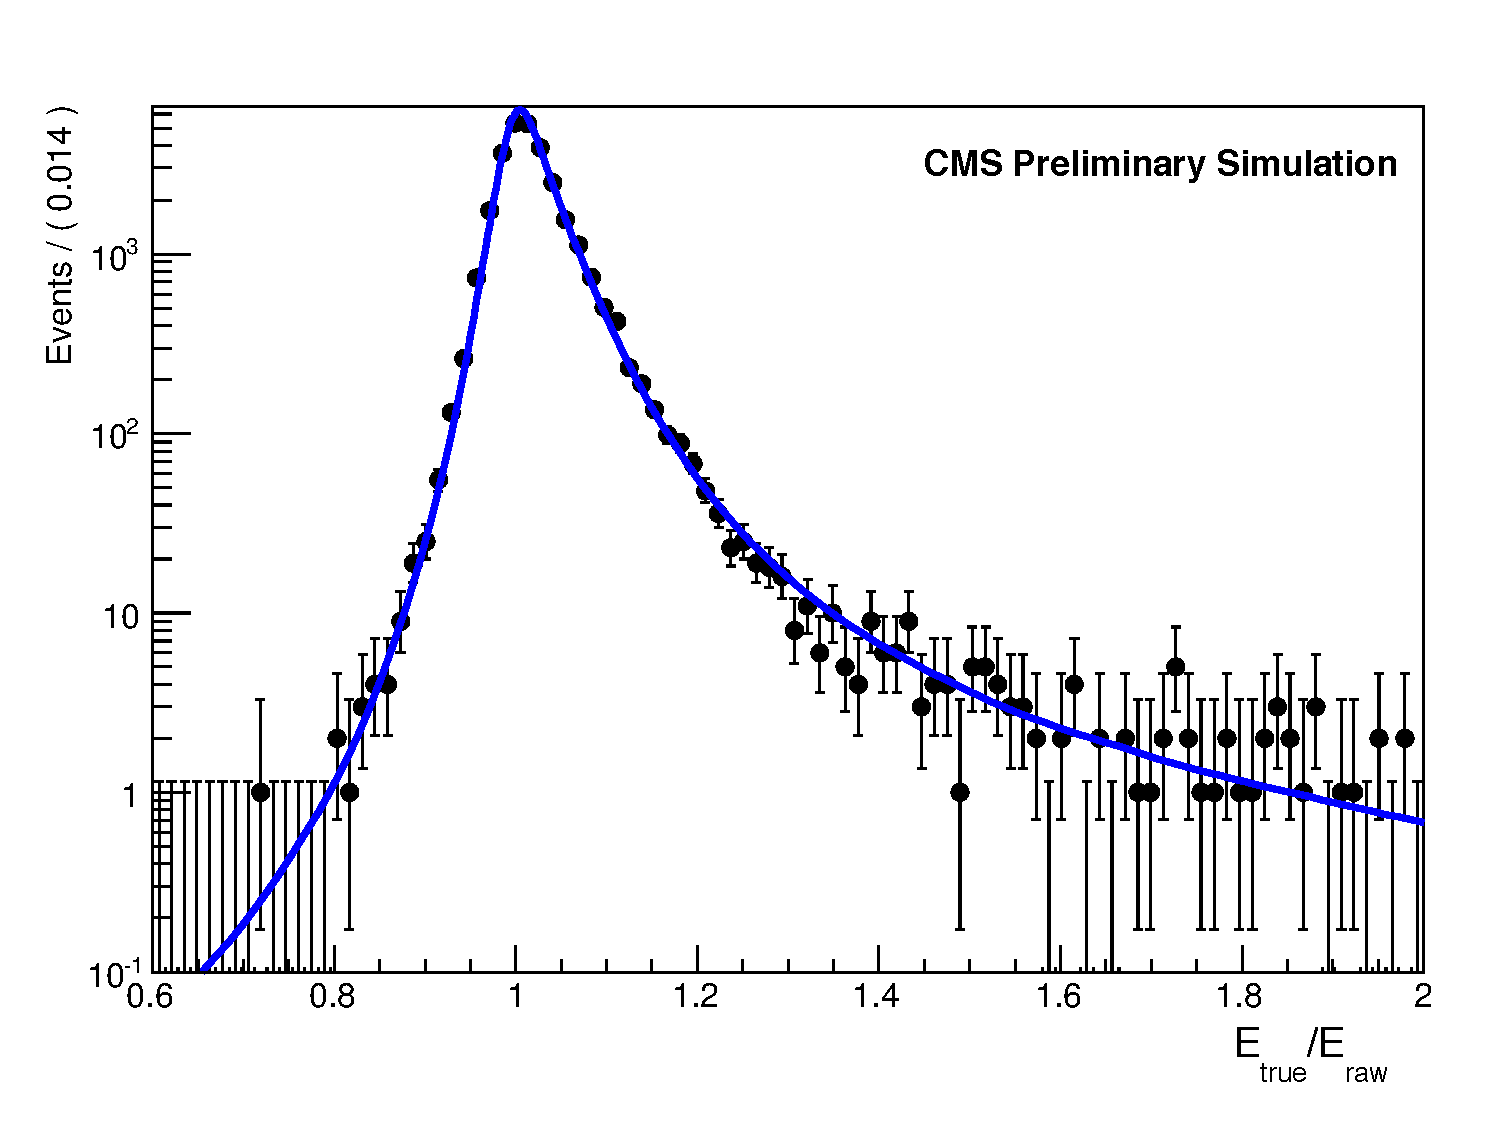
\includegraphics[width=0.48\textwidth]{analysis_comps/plots/regression_endcap_fix.pdf}
  \caption[A comparison of the predicted probability density of $E_{true}/E_{raw}$ from the regression training to the distribution in a statistically independent sample]{A comparison of the predicted probability density of $E_{true}/E_{raw}$ from the regression training (blue line) to the distribution in a statistically independent \MC sample (black points) for barrel photons (left) and endcap photons (right).}
  \label{fig:regression_training}
\end{figure}

\subsection{Correcting for residual discrepancies between data and Monte Carlo simulation}
\label{sec:scale_smearing}

After application of the energy regression correction there are some remaining discrepancies between data and \MC simulation. These residual effects are accounted for using \Zee events in data and simulation to correct the energy scale in the data and to apply an additional smearing term to the \MC events with systematic uncertainties propagated through the analysis to account for the uncertainties on these corrections.

\subsubsection{Energy scale corrections to the data}

The supercluster energy is identical for electrons and photons so by correcting the supercluster energy scale to a known source, namely the mass of the $Z$-boson, in dielectron decays the smaller residual energy scale effects are accounted for. When reconstructing the dielectron decays to derive these corrections, electrons are reconstructed as photons and the $Z$ mass calculated in the same way as for the diphoton invariant mass in Eq.~\ref{eq:dipho_inv_mass}, where the electron energy is obtained from the supercluster alone and the dielectron opening angle is obtained from the tracks. This can be done several times to account for various different effects. In the first stage scale corrections are derived in bins of time (run range) and \eta. After applying these corrections, further, much smaller, residual effects are accounted for in bins of \rnine (the size of the effect is different for converted and non-converted photons). After applying both of these a further step is taken for the 8 TeV data in the barrel to derive residual corrections in bins of \ET. Consequently the total scale correction is a product of three corrections in 59 bins of time $\times$ 4 bins in \eta $\times$ 2 bins in \rnine $\times$ 6 bins in \ET (where the last is applied for the 8~TeV barrel photons only).

The strategy for deriving these corrections is to take \Zee events in data and \MC simulation and extract the invariant dielectron mass in the relevant bin of interest. This mass distribution is fitted with a convolution of a relativistic Breit-Wigner (designed to handle the underlying Z line shape~\cite{pdg}) and a Crystal Ball function which models the calorimeter resolution effects and bremsstrahlung losses in the material upstream of the \ECAL. The Breit-Wigner parameters are fixed to the PDG values of $M_{Z}=91.188$~\GeV and $\Gamma_{Z}=2.495$~\GeV~\cite{pdg} whilst the Crystal Ball parameters which model the detector effects are allowed to float. The scale correction, $\Delta E$, is then defined as the relative difference between the Crystal Ball peak in data and simulation,
\begin{equation}
  \Delta E = \frac{m_{data}-m_{MC}}{M_{Z}}.
\end{equation}
\subsubsection{Energy resolution smearing for the Monte Carlo events}

A similar method is used to extract a smearing factor that can be applied to the \MC events such that the width of the invariant mass distribution in \Zee decays matches between data and \MC events. This is done in 4 bins of \eta $\times$ 2 bins of \rnine and is parametrised as the quadratic sum of two resolution components: a constant term, $\Delta C$, and a stochastic term, $\Delta S$, which aims to model the expected resolution effects explained in Eq.~\ref{eq:energy_res} in Sec.~\ref{sec:ecal}. The smearing term, $\Delta\sigma$, is parametrised as,
\begin{equation}
  \Delta\sigma = \frac{\Delta S}{\sqrt{E_{T}}} \oplus \Delta C.
\end{equation}
The effect of the scale and smearing corrections is shown for the \Zee data and \MC samples in Fig.~\ref{fig:scale_smearing_Zee}. Figure~\ref{fig:scale_smearing_analysis} shows the \Zee invariant mass distribution for data and \MC events at 8~TeV for events passing the analysis preselection. The discrepancy between the data and the \MC simulation in the tails of the dielectron invariant mass distribution, shown in the right hand plot of Fig.~\ref{fig:scale_smearing_analysis}, is considerably reduced (from $\sim20\%$ to $\sim10\%$) after the full analysis event selection is made (not just the preselection shown here). Furthermore the analyis sensitivty is decreased by less than 5\% when events with at least one photon in the endcap are removed and consequently the remaining discrepancy is not considered as significant. Each of the scale and resolution corrections has an associated uncertainty and these uncertainties are propagated per photon through the analysis. There are also additional uncertainties included which account for differences between electrons and photons and the difference between the $Z$ mass scale (around 90~\GeV) and the Higgs mass scale (around 125~\GeV). Systematic uncertainties are described in more detail in Sec.~\ref{sec:systematics}.

\begin{figure}
  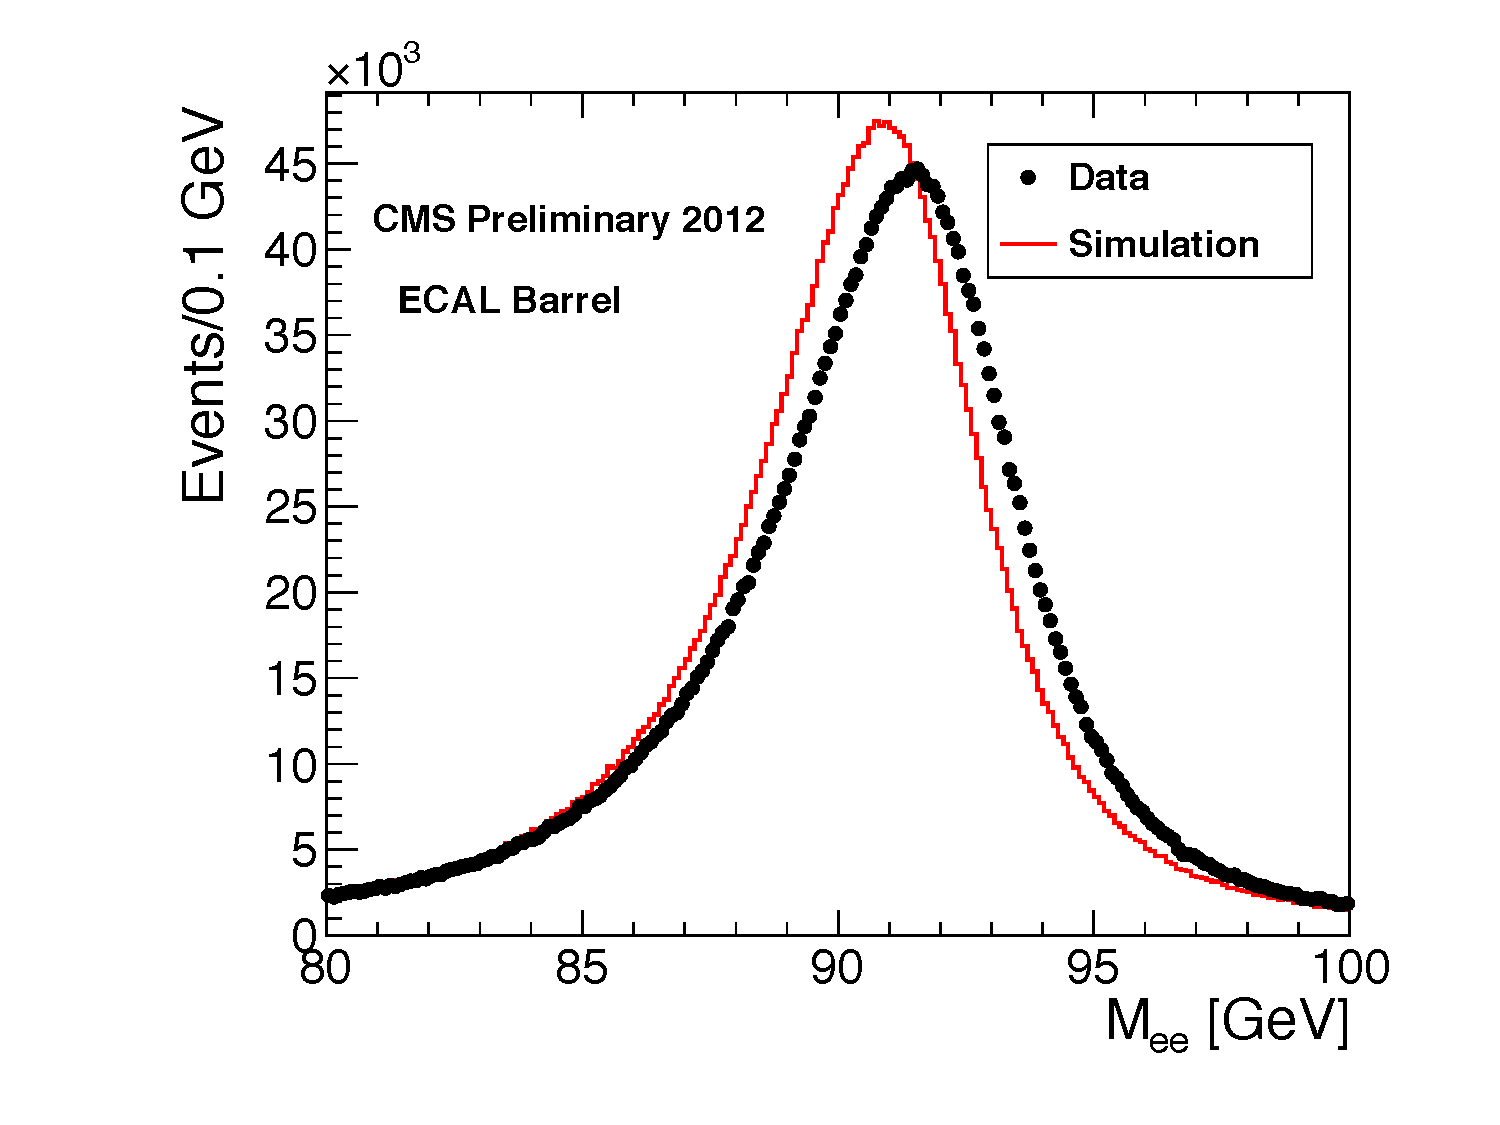
\includegraphics[width=0.48\textwidth]{analysis_comps/plots/zee_beforecorr_fix.pdf}
  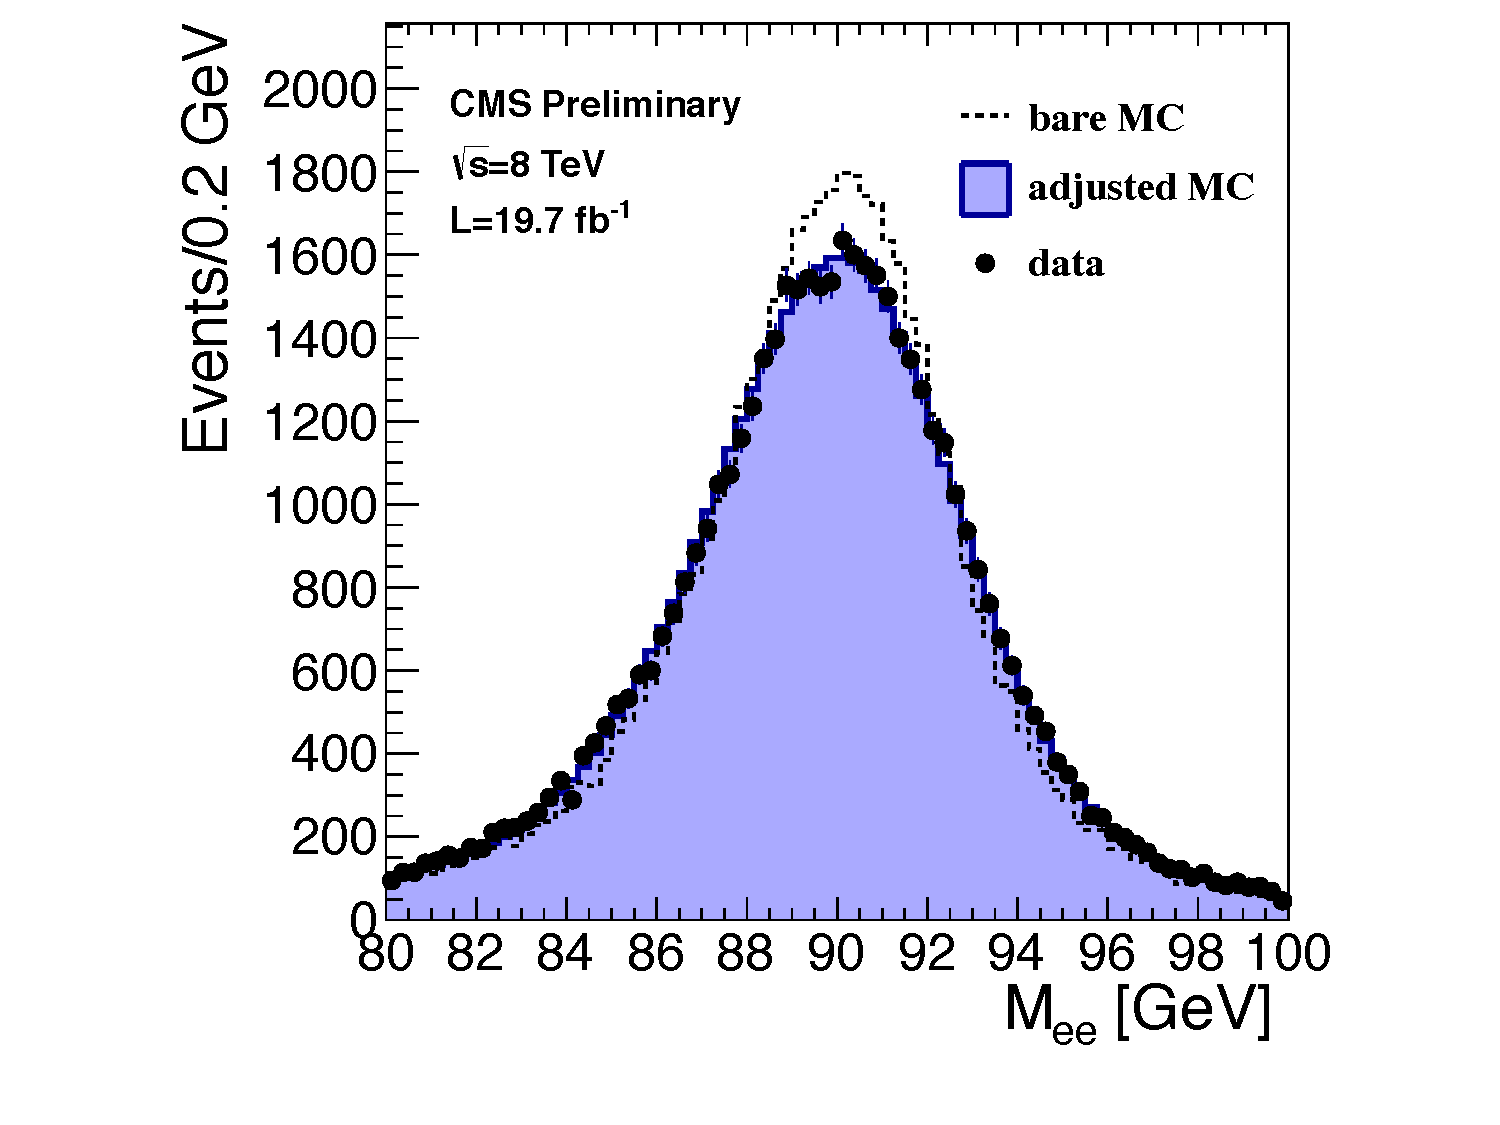
\includegraphics[width=0.48\textwidth]{analysis_comps/plots/zee_aftercorr_fix.pdf}
  \caption[The \Zee invariant mass shape before and after scale and smearing corrections are applied]{The \Zee invariant mass shape comparison of data and MC events before (left) and after (right) the scale and smearing corrections are applied. Shown for 8~TeV electrons (reconstructed as photons) in the barrel.}
  \label{fig:scale_smearing_Zee}
\end{figure}

\begin{figure}
  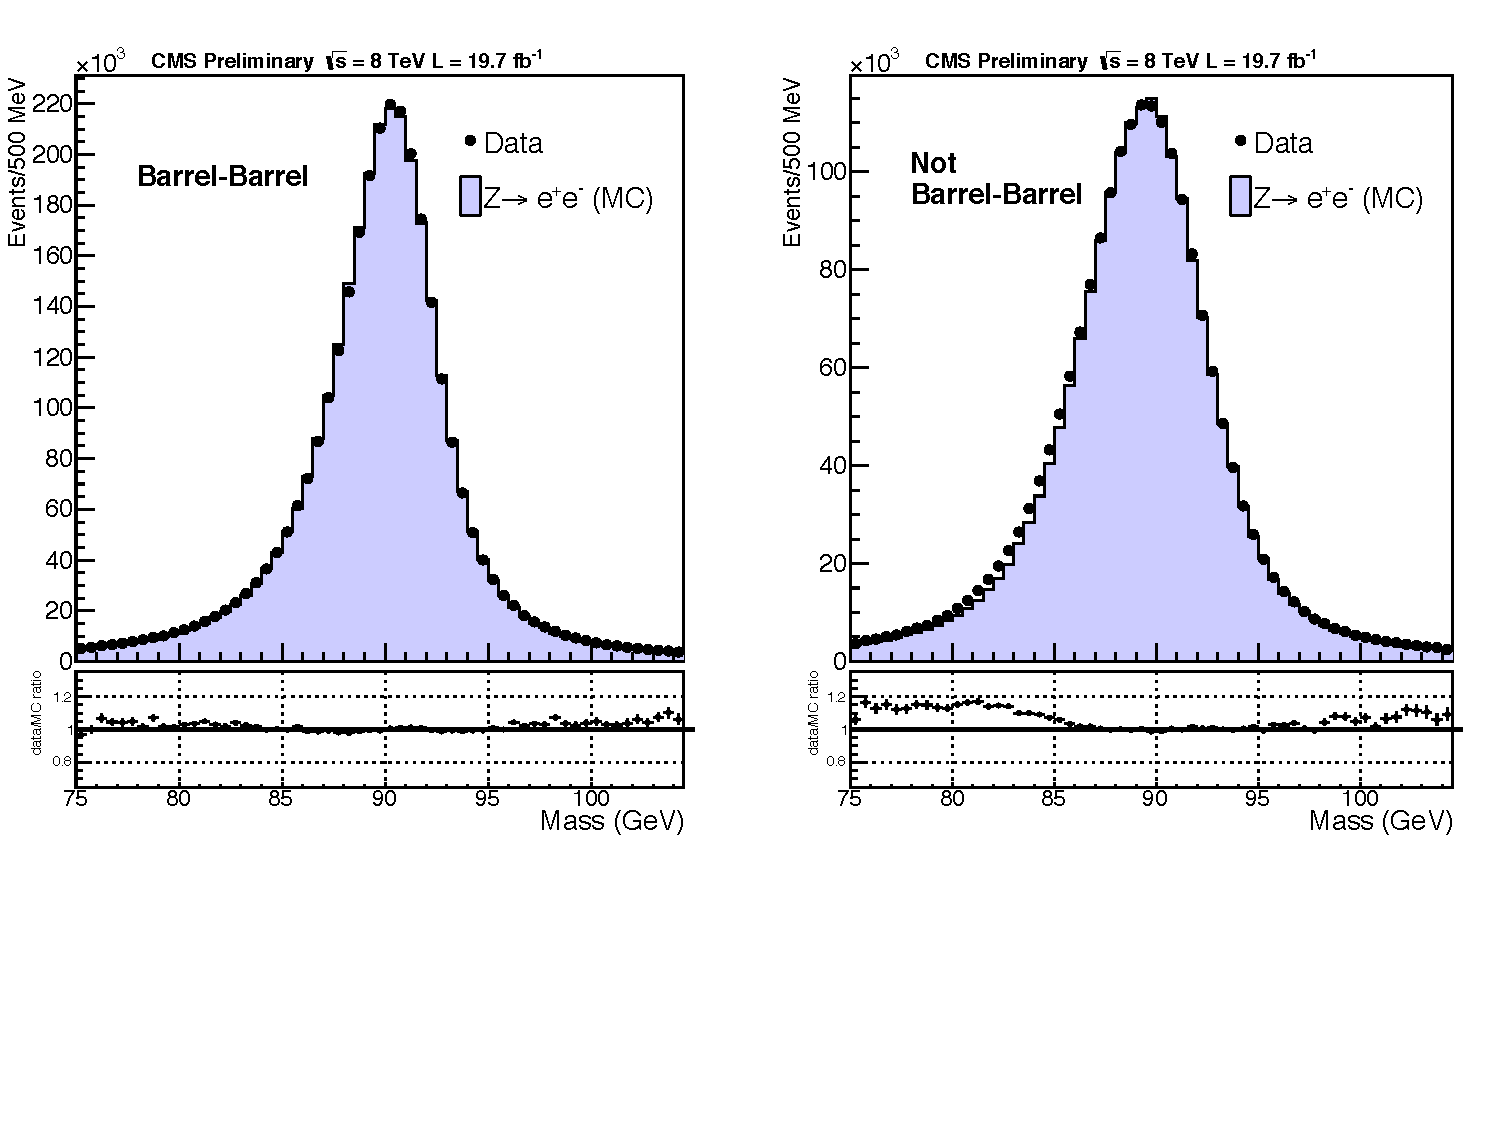
\includegraphics[width=0.99\textwidth]{analysis_comps/plots/massEBEE_fix.pdf}
  \caption[The \Zee invariant mass distribution at 8~TeV when the electrons are reconstructed as photons]{The \Zee invariant mass distribution at 8~TeV for electrons reconstructed as photons when both electrons are in the barrel (left) and when at least one is not in the barrel (right). Shown for data (black points) and \MC events (blue histogram) which pass the analysis preselection when the electron veto is inverted.}
  \label{fig:scale_smearing_analysis}
\end{figure}

\section{Vertex reconstruction}
\label{sec:vtx_reco}

The resolution on the opening angle has a negligible effect if the correct vertex can be found within 10~mm of the true interaction point. As seen in Sec.~\ref{sec:pileup_beamspot} the beamspot has an RMS spread of about 5~cm in the $z$ direction and there is an average of $\sim20$ vertices per bunch crossing. Because the beam direction is along the $z$-axis the spread of the vertex in the $x$ and $y$ directions is tiny ($<0.5$~mm) and consequently mismeasurement of the primary vertex in the $x$-$y$ plane is small and has no impact on the mass resolution. By assigning the correct vertex to the diphoton pair, using other information in the tracking system, most of the mass resolution can be preserved. The method used to extract the primary vertex is a classification \BDT which exploits the correlation between the diphoton pair and the recoiling tracks from the underlying interaction as well as additional information in the tracking system if there is a photon conversion pair. The output of this per-vertex \BDT is evaluated for each vertex in the event and the primary vertex is assigned as the one with the highest value of the \BDT output (i.e.\ the value nearest 1.). In addition, it is possible to construct another \BDT whose output is proportional to the probability that the chosen vertex is the correct one (described in Sec.~\ref{sec:bdt_prob}). This probability becomes a useful discriminating variable for the analyses later on.

The vertex \BDT uses the following input variables:

\begin{itemize}
  \item $\sum\limits_{i} |\vec{p}{}^{\;i}_{T}|^{2}$ - the sum of the transverse momentum squared of all of the tracks which originate from this vertex, representing how hard the interaction is at this vertex.
  \item $\frac{\vec{p}^{\gamma\gamma}_{T}}{|\vec{p}^{\gamma\gamma}_{T}|} \cdot \sum\limits_{i} \vec{p}_{T}^{i}$ - the dot product between the transverse momentum of the diphoton system and the sum of all other tracks originating from this vertex, representing the recoil of the tracks relative to the diphoton system.
  \item $\bigr(|\sum\limits_{i} \vec{p}^{\;i}_{T}| - |\vec{p}^{\gamma\gamma}_{T}|\bigl) / \bigr(|\sum\limits_{i} \vec{p}{}^{\;i}_{T}| + |\vec{p}^{\gamma\gamma}_{T}|\bigl)$ - the asymmetry between the diphoton system and the other tracks originating from this vertex.
  \item $|z_{v}-z_{c}|/\sigma_{c}$ - this is added for events which contain at least one photon conversion where $z_{v}$ is the $z$ position of the vertex in question and $z_{c}$ and $\sigma_{c}$ are the estimated $z$ position of the vertex from conversion information and its approximate error as defined below.
\end{itemize}

For events which contain at least one photon conversion, the conversion tracks and/or the conversion momentum can be used to point back to the beam line and estimate the vertex position. This can be achieved in one of two ways. In cases where the conversion occurs early, i.e.\ in one of the first layers of the tracking system, then the electron pair from the conversion will leave two clean and distinct tracks. This means that the momentum of the conversion pair can be accurately reconstructed and used to point from the conversion vertex position back to the beam line and thus the nearest primary vertex. In cases where the conversion occurs late in the tracking system, there are not enough track hits to accurately reconstruct the momentum of the conversion pair. However the incident position of the photon at the \ECAL face is well known in this case, so the line which connects the \ECAL position with the conversion vertex can be used to point back to the beam line. This is diagrammatically represented in Fig.~\ref{fig:conv_diags} for both cases.

\begin{figure}
  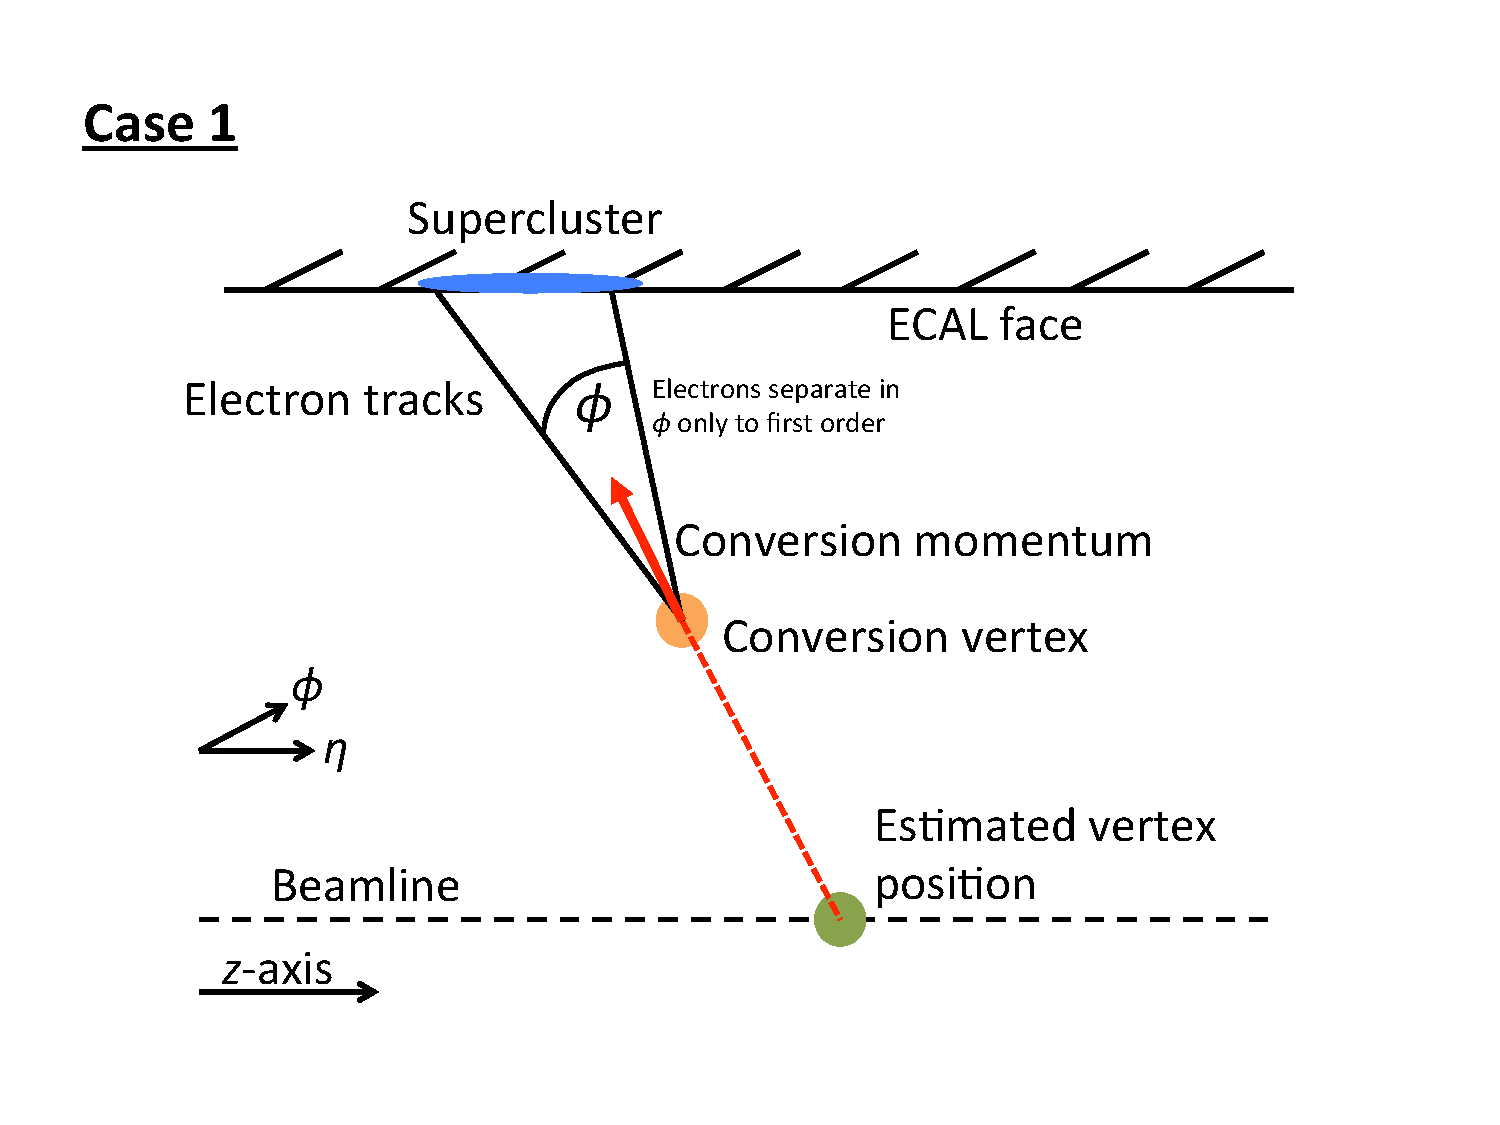
\includegraphics[width=0.49\textwidth]{analysis_comps/plots/ConvDiagNewCase1.pdf}
  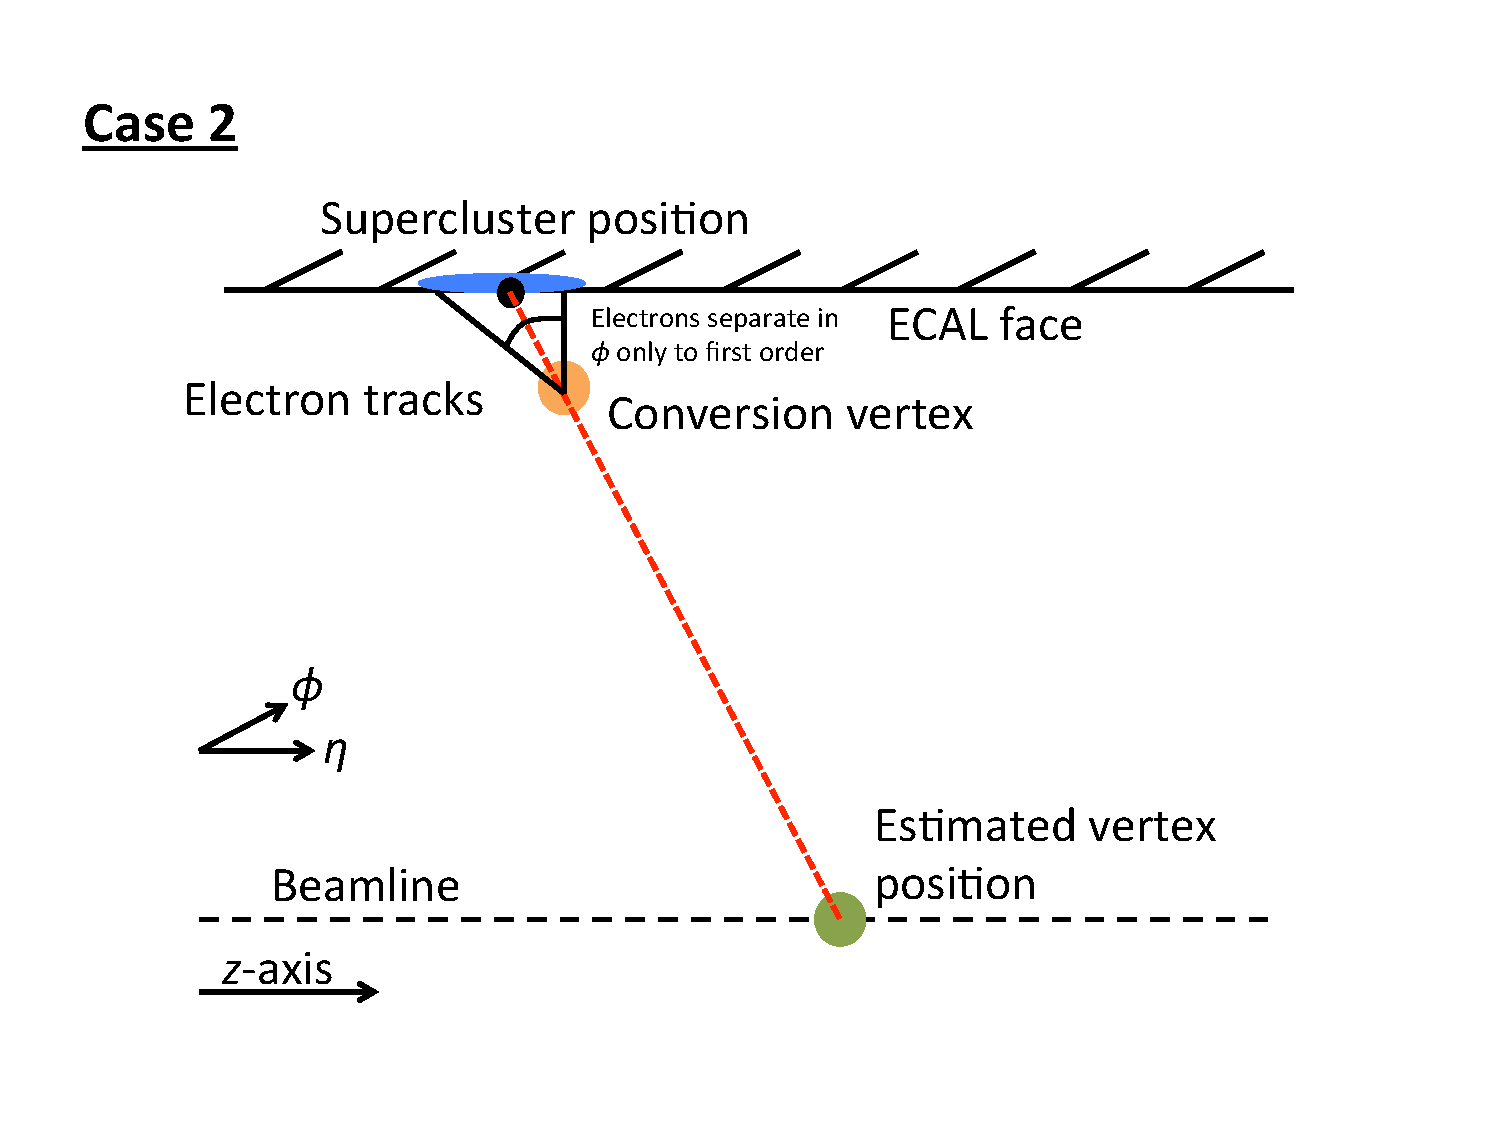
\includegraphics[width=0.49\textwidth]{analysis_comps/plots/ConvDiagNewCase2.pdf}
  \caption[A schematic showing the two methods used for locating the primary vertex]{A representation of the two methods for locating the primary vertex using photon conversion information. The left plot is for cases where the conversion occurs early enough in the tracker that the two electron tracks can be used to construct the converted pair momentum, which is then combined with the conversion vertex position to point back to the beam line. The right plot is for cases where the conversion occurs late in the tracker and the energy weighted supercluster position and the conversion vertex position are used to point back to the beam line.}
  \label{fig:conv_diags}
\end{figure}

For Case 1 conversions the primary vertex $z$ position is calculated as,
\begin{equation}
  z_{c} = z_{conv} - r_{conv}\cot(\alpha),
\end{equation}
where $z_{conv}$ is the $z$ position of the conversion vertex, $r_{conv}$ is the distance of the conversion vertex from the beam line and $\alpha$ is the angle between the beam line and the conversion momentum.

For Case 2 conversions the primary vertex $z$ position is calculated as,
\begin{equation}
  z_{c} = \frac{r_{conv}z_{SC} - r_{SC}z_{conv}}{r_{conv} - r_{SC}},
\end{equation}
where $z_{conv}$ and $z_{SC}$ are the $z$ positions of the conversion vertex and supercluster respectively, and $r_{conv}$ and $r_{SC}$ are the distance of the conversion vertex and the supercluster from the beamline.

There are six regions of the tracking system (refer back to Fig.~\ref{fig:cms_tracker}). When the conversion vertex is located in one of the inner regions; Pixel Barrel, Pixel Forward or TID, the Case 1 
conversion information is included in the \BDT, otherwise the Case 2 conversion information is used. The resolution on the primary vertex position in conversions is estimated per tracking region using \gjet events in data for which the primary vertex efficiency is high and the photon converts. Using these events, the conversion resolution, $\sigma_{c}$, is calculated as the effective width\footnote{Half the narrowest interval which contains 68.3\% of the distribution} of the distribution of the difference, $\Delta z=z_{v}-z_{c}$, between the estimated $z$ position of the primary vertex without any conversion information, $z_{v}$, and the estimated $z$ position of the primary vertex when using conversion information alone, $z_{c}$. Consequently the fourth input variable to the \BDT, shown in the list above as $|z_{v}-z_{c}|/\sigma_{c}$, is effectively a pull distribution for the conversion vertex. The \BDT will favour vertices whose value of this variable is near zero.

The \BDT is trained on a sample of \Hgg \MC events. It is tested with a statistically independent sample and further validated using \Zmumu decays in data and \MC samples. The efficiency is measured in data using the \Zmumu channel where the muon tracks are removed from the \BDT variables to simulate a diphoton-like situation in data. The \BDT response is shown for \Zmumu data and \MC events for both the signal (right vertex) and background (wrong vertex) in Fig.~\ref{fig:vertex_bdt_response}. The chosen primary vertex is the one which gives the highest score \BDT output. The efficiency of the vertex selection as a function of the $Z$ \pT and the number of reconstructed vertices as measured in \Zmumu data and \MC samples is shown in Fig.~\ref{fig:vertex_bdt_efficiency}. 

\begin{figure}
  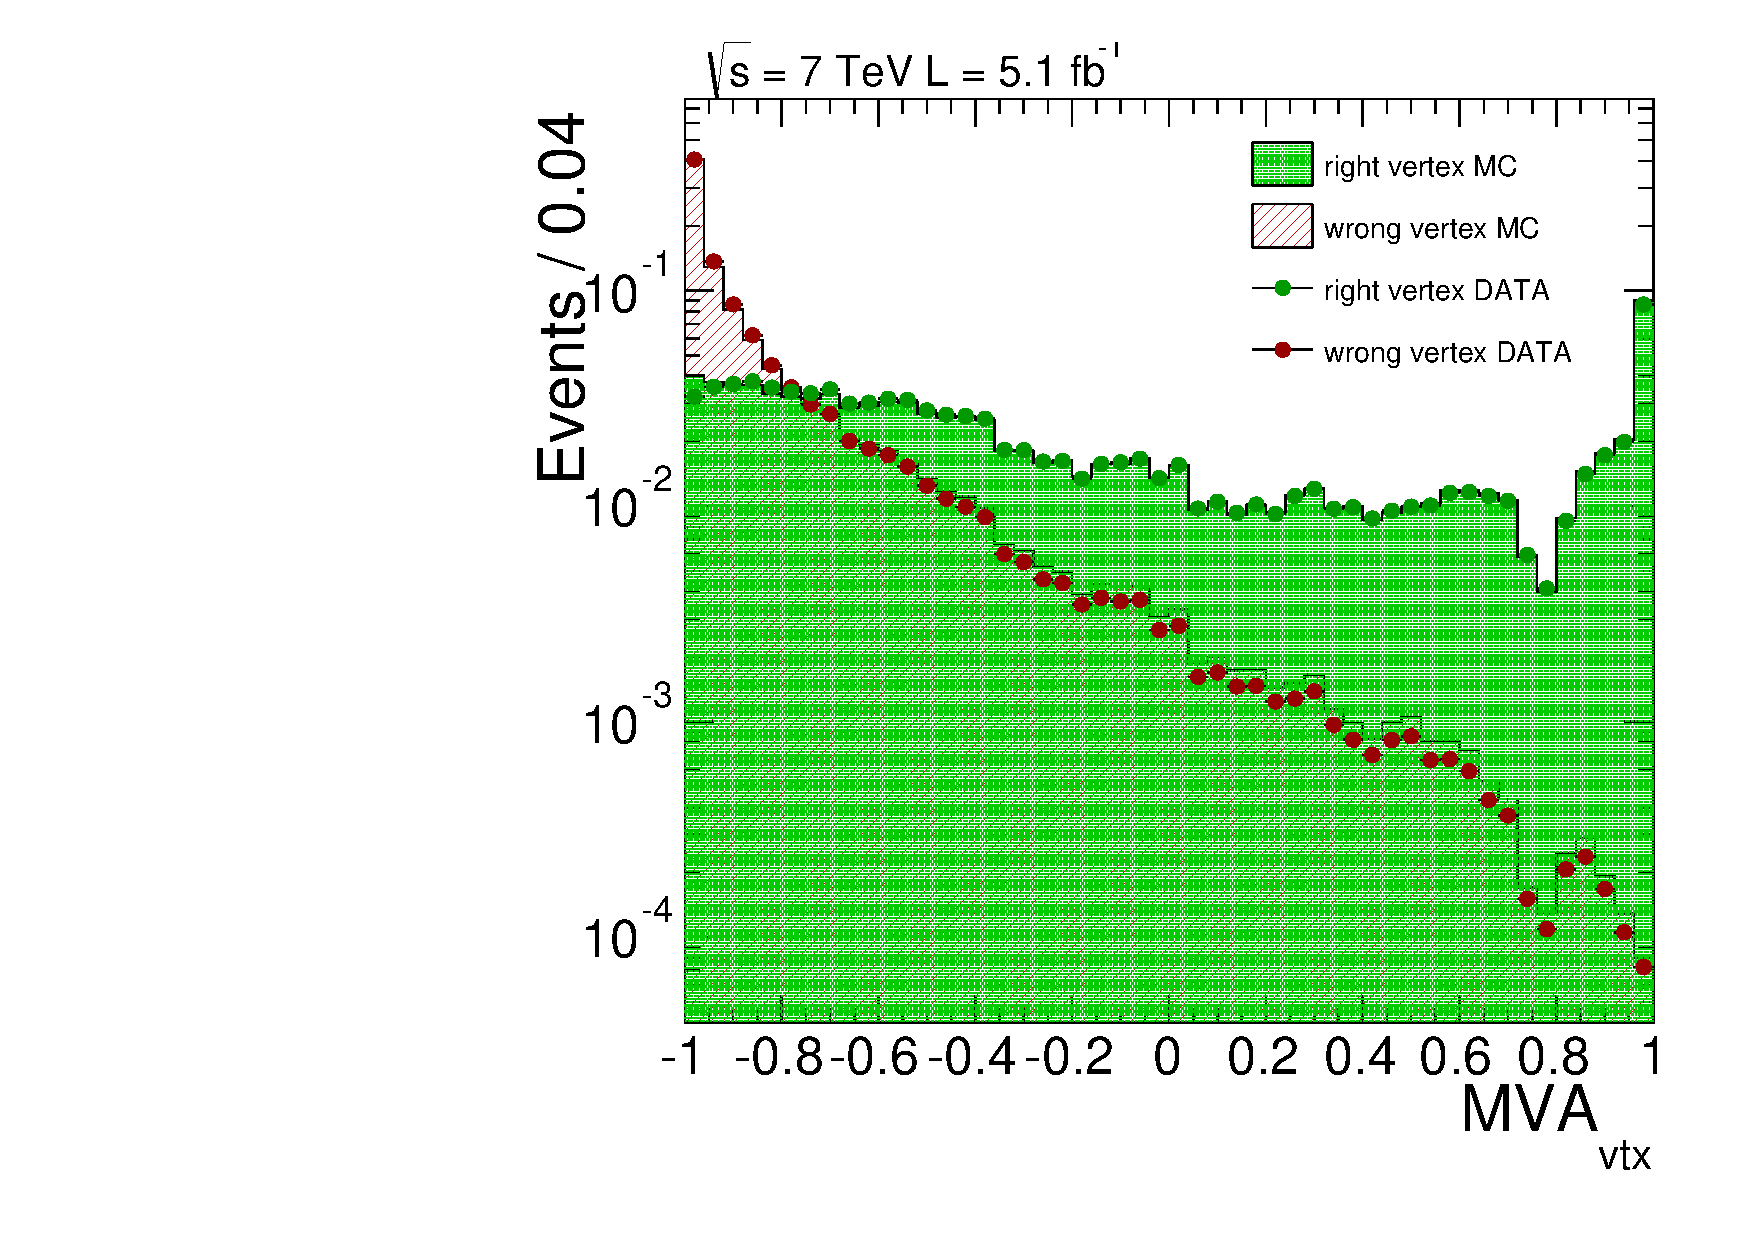
\includegraphics[width=0.48\textwidth]{analysis_comps/plots/vertex_bdt_output_7TeV_log.pdf}
  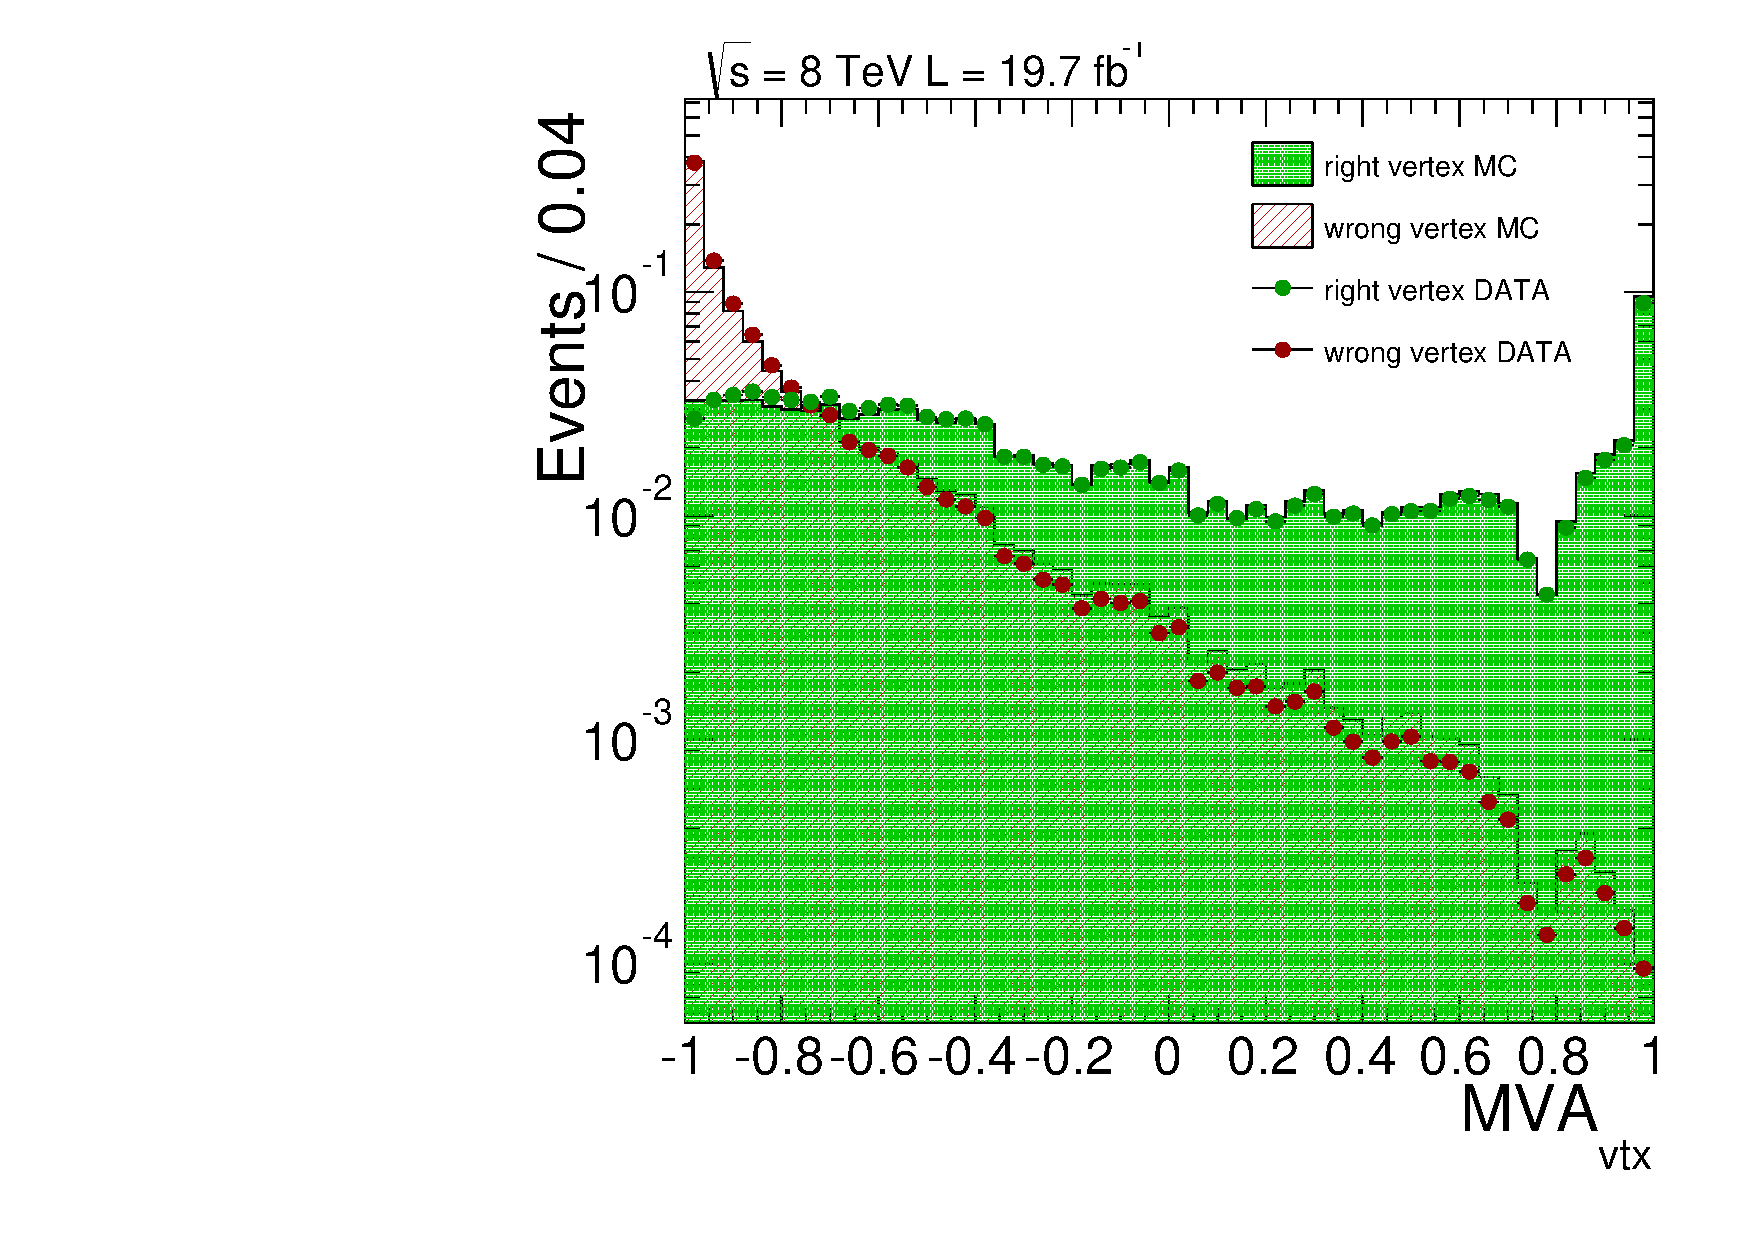
\includegraphics[width=0.48\textwidth]{analysis_comps/plots/vertex_bdt_output_8TeV_log.pdf}
  \caption[The vertex \acs{BDT} response for \Zmumu events]{The vertex \BDT response for \Zmumu events in data (points) and MC events (filled histogram) for the primary vertex (green) and the background pileup vertices (red).}
  \label{fig:vertex_bdt_response}
\end{figure}

\begin{figure}
  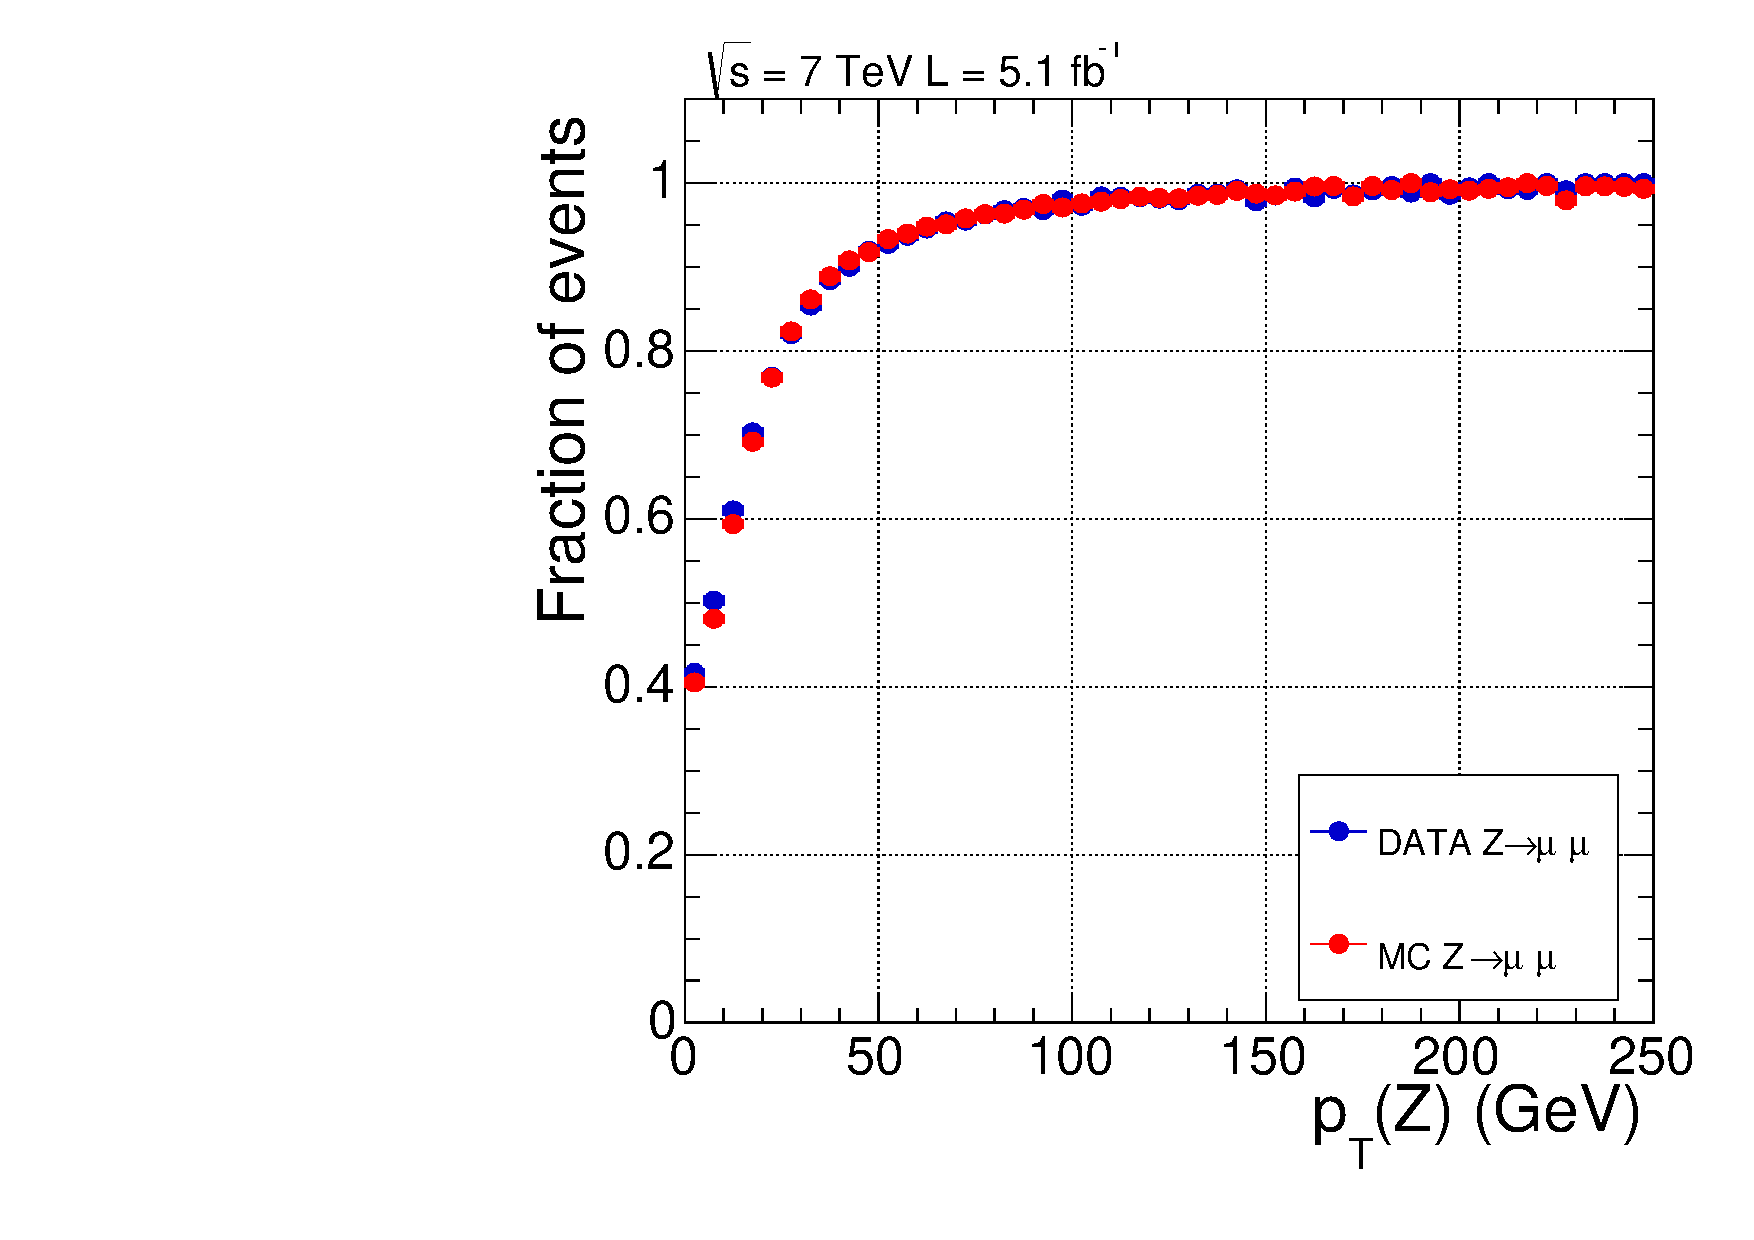
\includegraphics[width=0.48\textwidth]{analysis_comps/plots/vertex_bdt_efficiency_pt_7TeV.pdf}
  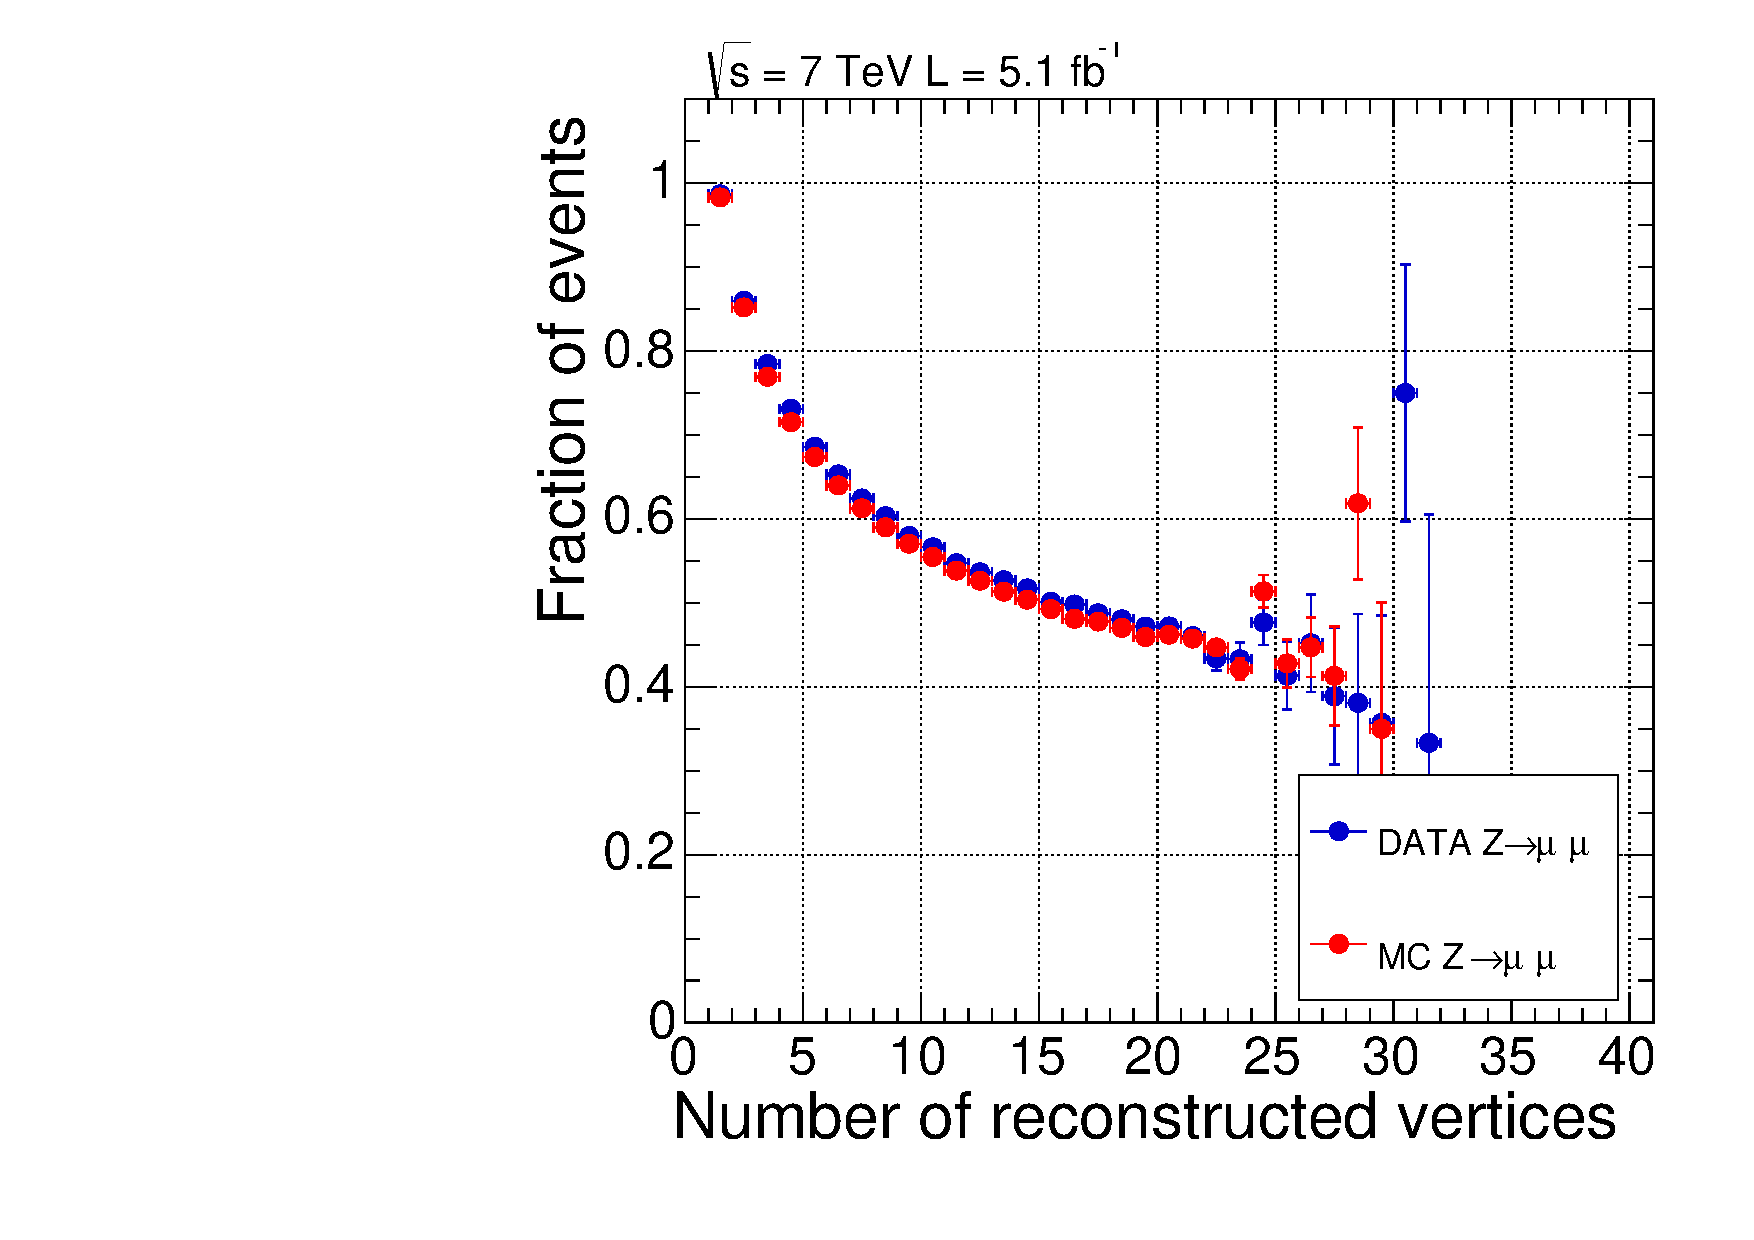
\includegraphics[width=0.48\textwidth]{analysis_comps/plots/vertex_bdt_efficiency_nvtx_7TeV.pdf} \\
  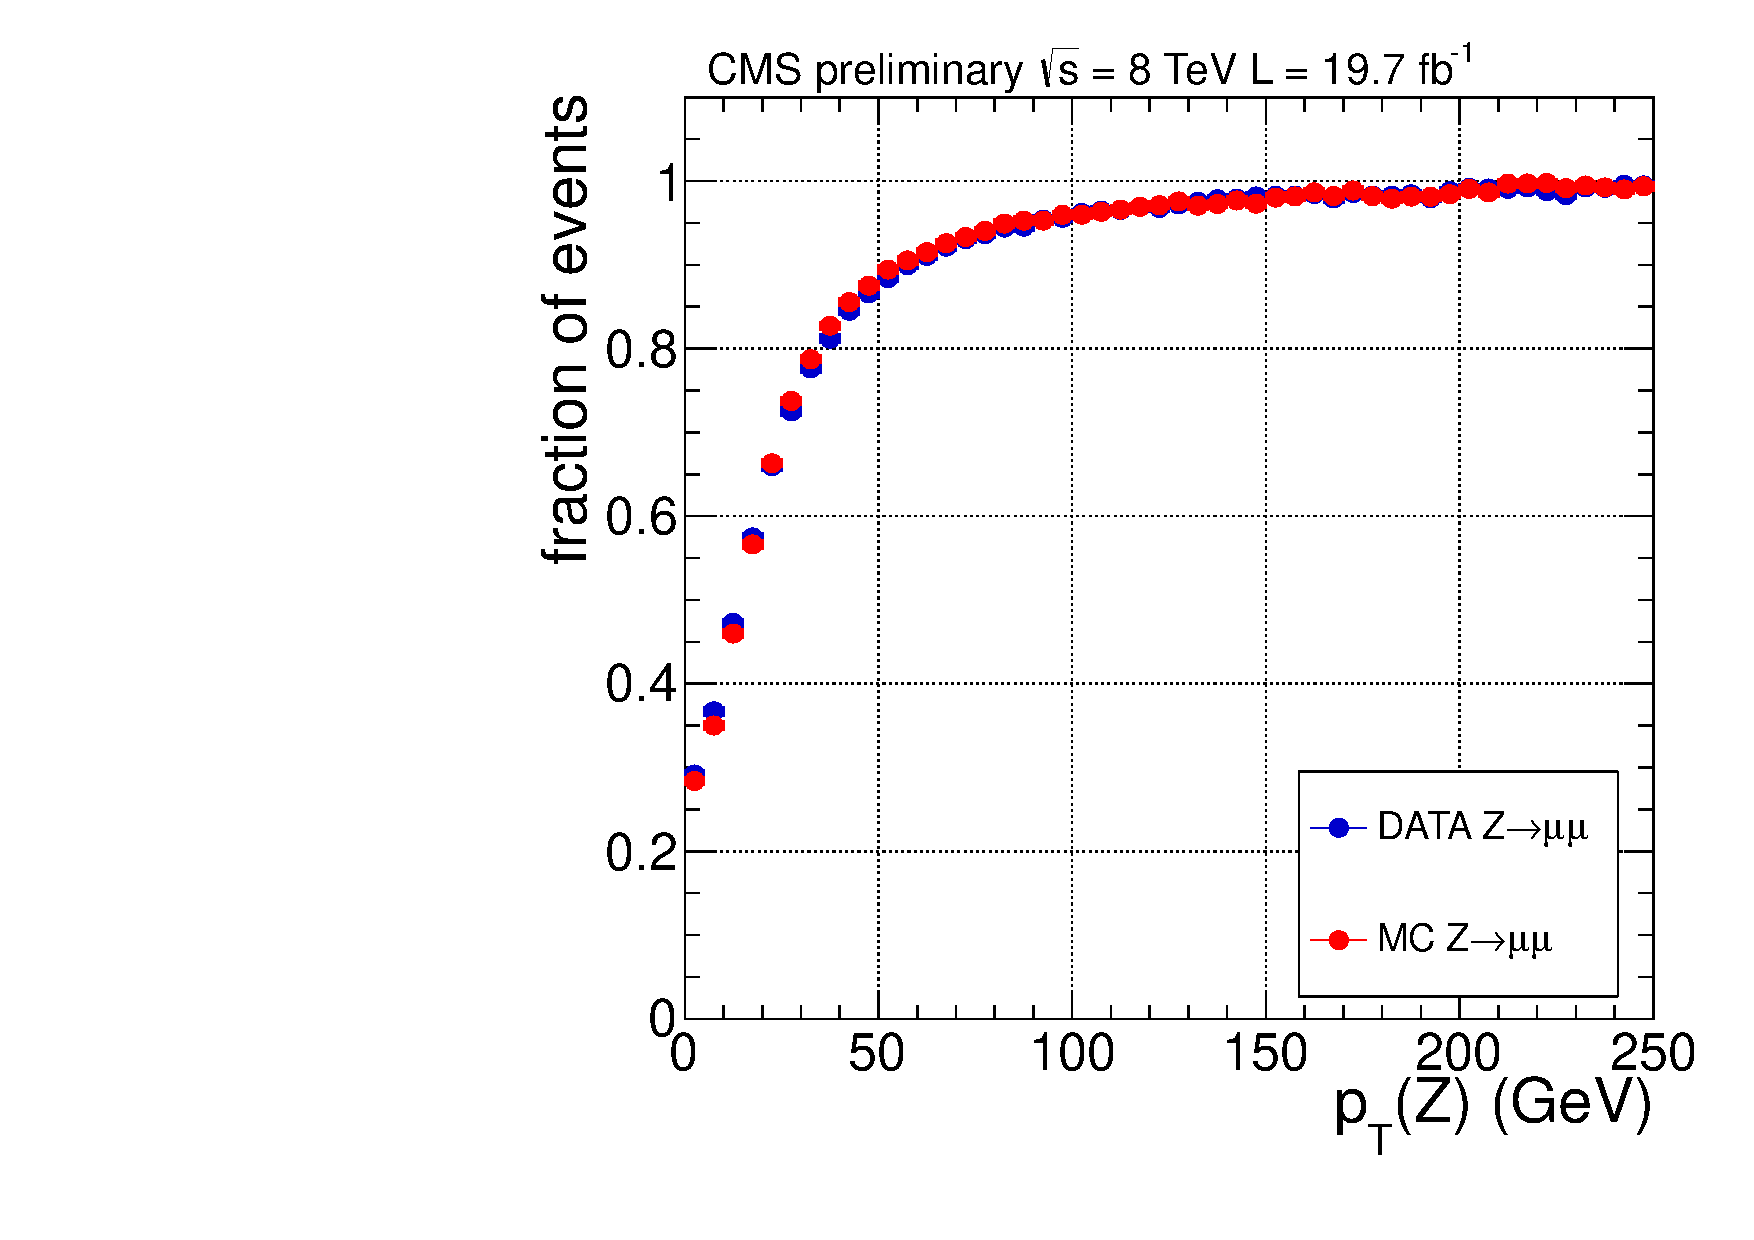
\includegraphics[width=0.48\textwidth]{analysis_comps/plots/vertex_bdt_efficiency_pt_8TeV.pdf}
  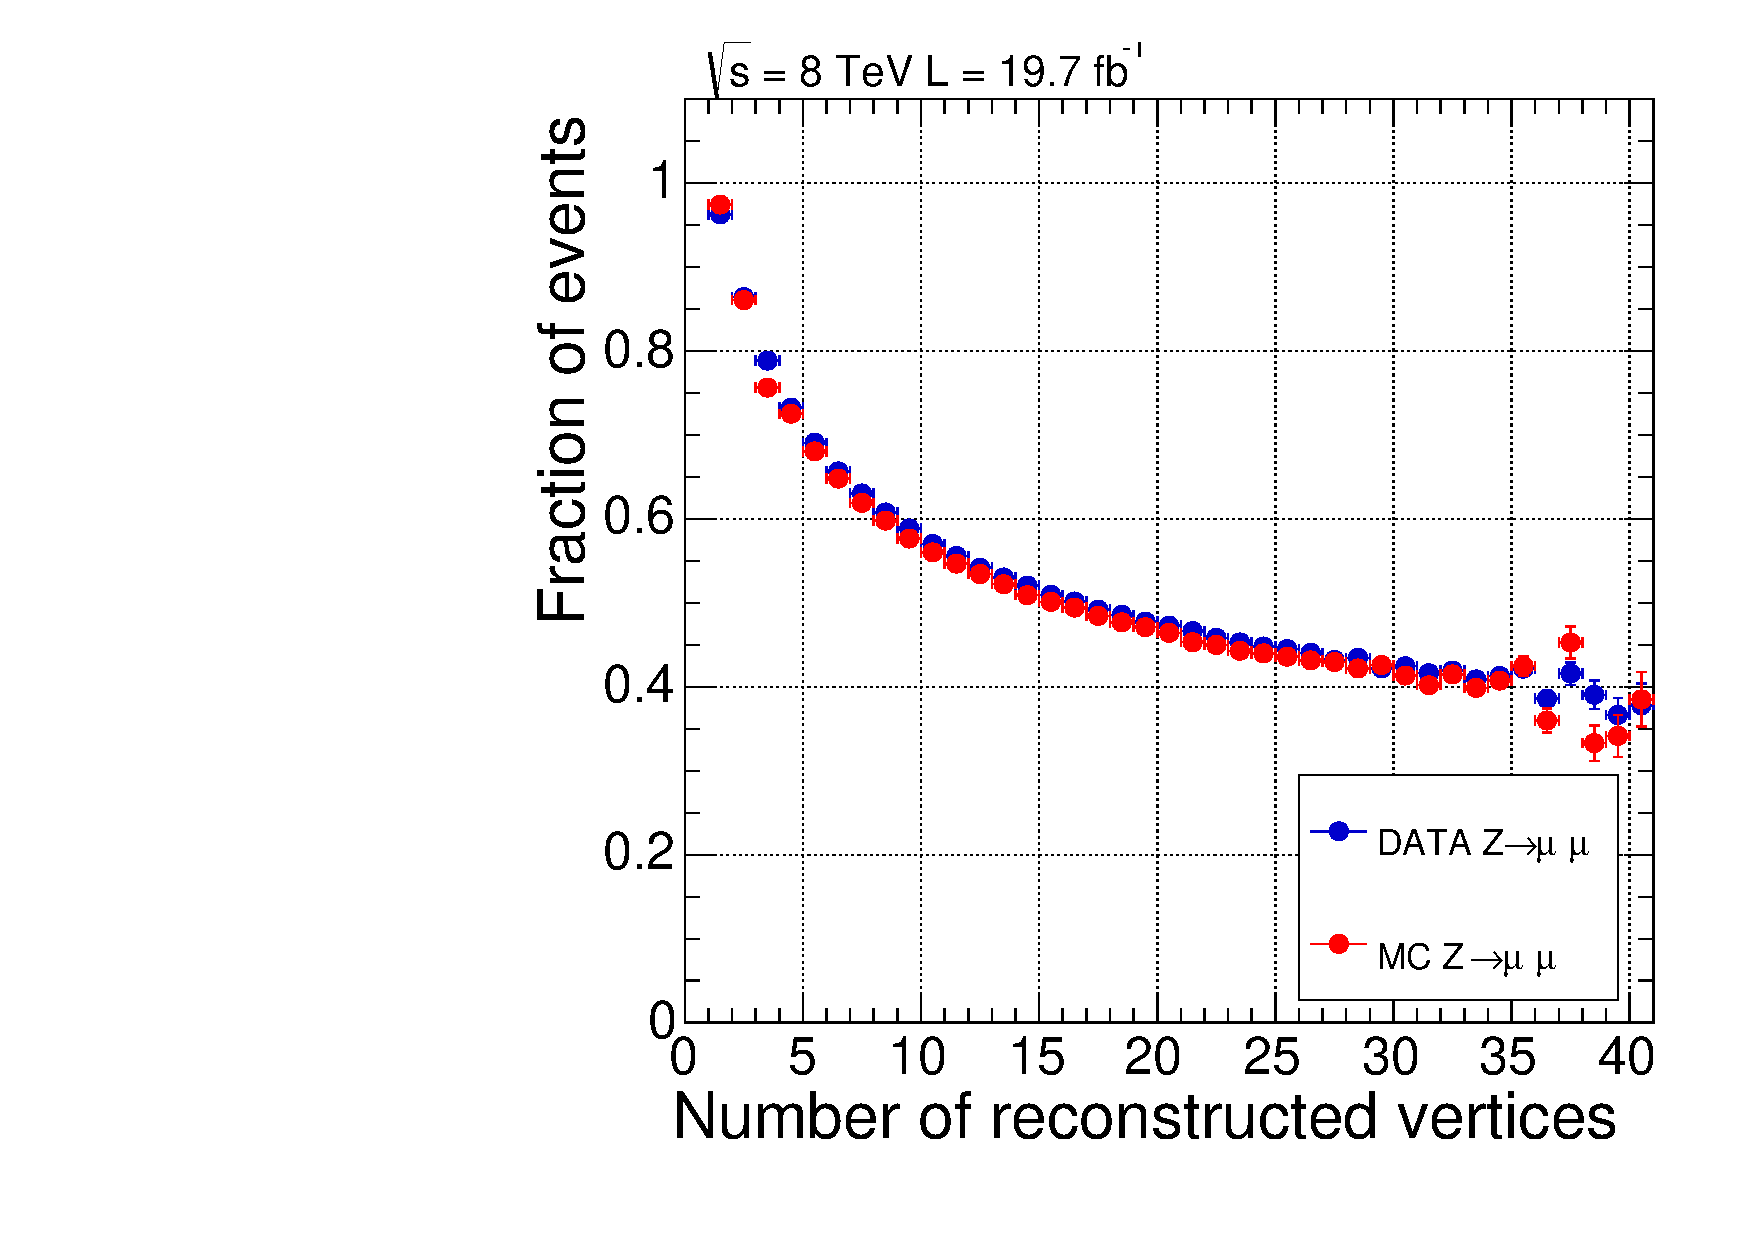
\includegraphics[width=0.48\textwidth]{analysis_comps/plots/vertex_bdt_efficiency_nvtx_8TeV.pdf} 
  \caption[The efficiency of locating the correct vertex]{The chosen vertex efficiency as measured in \Zmumu data and \MC simulation as a function of $Z$ \pT (left) and number of reconstructed vertices (right) for the 7~TeV (top row) and 8~TeV (bottom row) data samples.}
  \label{fig:vertex_bdt_efficiency}
\end{figure}

\subsection{Estimating the per-event probability that the correct vertex is chosen}
\label{sec:bdt_prob}

The total efficiency for assigning the correct vertex using the method described in the preceding section is at the level of 75\% during 2012 running conditions, where the correct vertex is defined as being within 10~mm of the true vertex. This means that for around 25\% of preselected events the mass resolution is dominated by the vertex resolution. Consequently, it is important to ascertain the probability that the chosen vertex is the correct one. An additional specific \BDT is constructed to address exactly this topic. The input variables used for this \BDT are:

\begin{itemize}
  \item the \pT of the diphoton system;
  \item the number of vertices in each event;
  \item the value of the per-vertex \BDT described above, for the three vertices with the highest score;
  \item the $z$ distance, $\Delta z$, between the chosen vertex and the second and third choice vertices;
  \item the number of photon conversions used; either 0, 1 or 2.
\end{itemize}

There is a linear relation between the response of this \BDT and the correct vertex efficiency (or probability). This is used to analytically obtain the per-event correct vertex probability for a given event. Figure~\ref{fig:vertex_bdt_prob_efficiency} shows that this estimation reproduces the required vertex efficiency as a function of Higgs \pT and number of reconstructed vertices.

\begin{figure}
  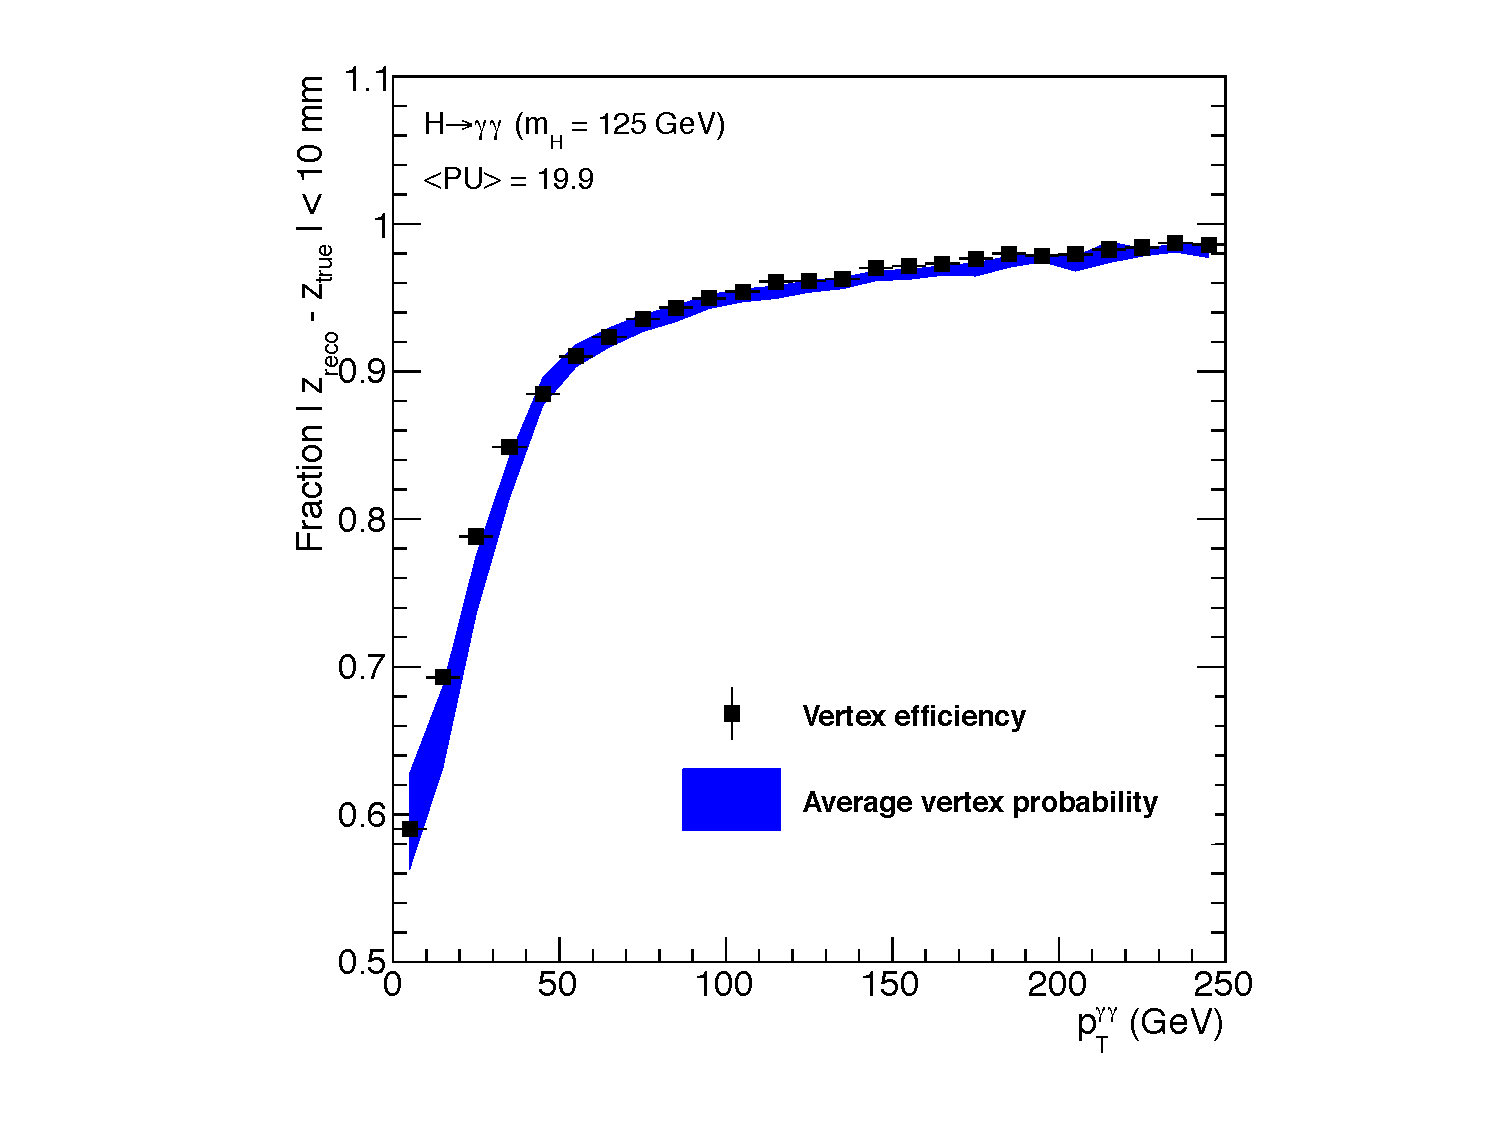
\includegraphics[width=0.48\textwidth]{analysis_comps/plots/vtxProbPt.pdf}
  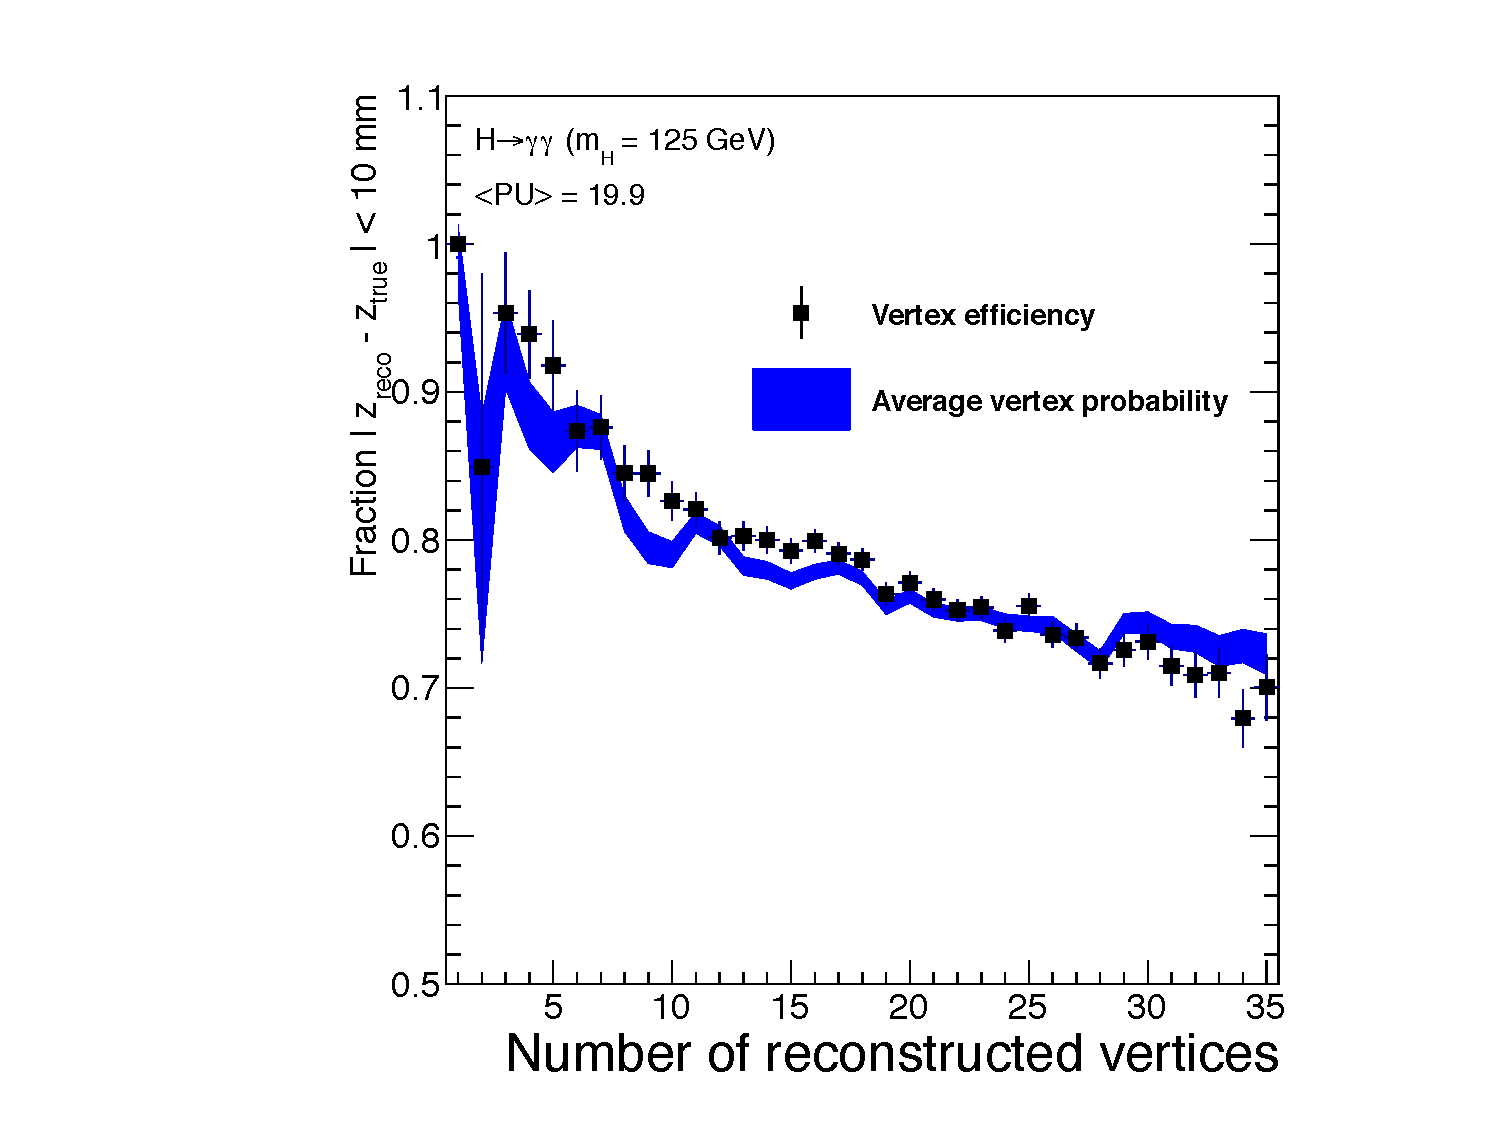
\includegraphics[width=0.48\textwidth]{analysis_comps/plots/vtxProbNvtx.pdf}
  \caption[A comparison of the true vertex efficiency and the average vertex probability]{A comparison of the true vertex efficiency (black points) and the average vertex probability (blue band) for a statistically independent \MC Higgs sample simulated with 2012 running conditions.}
  \label{fig:vertex_bdt_prob_efficiency}
\end{figure}

\section{Event preselection}
\label{sec:photon_presel}

A simple and loose preselection is applied to all photons before they enter the analysis. The preselection requirements are identical for all analysis approaches and are designed to remove some \emph{fake} photons whilst maintaining near 100\% trigger efficiency. The variables used for preselection are defined below and the preselection cuts are described in Table~\ref{tab:preselection}.

\begin{itemize}
  \item $H/E$ - The ratio of hadronic energy in the \HCAL tower behind the supercluster to the electromagnetic energy in the supercluster. Neutral jets which fake photons typically leave a fraction of their energy in the \HCAL so there is a requirement that the value of this variable is small.
  \item $\sigma^{2}_{i\eta i\eta}$ - The RMS spread of the shower in the $\eta$ direction. Multiple showers of a \pizero, or more than one \pizero, result in a wider shower in \eta (as the \pizero decay product photons are separated in space). This cannot be exploited in the \phi direction because conversion electrons get separated by the magnetic field, however single photons, even when converted, occupy a narrow region in \eta. The separation of the two photons from a \pizero is minimal when they share the energy equally and given that typically $p_{T}\gg m_{\pi}$ the separation is close to minimal for most \pizero decays. Taking the transverse plane in the barrel, the separation $d=2Rm_{\pi}/p_{T}$ (where $R$ is the radius of the barrel), which for $p_{T}=40$~GeV gives a value of $d=$8~mm$\sim0.006$ in $\eta$. By referring to Table~\ref{tab:preselection} it is clear that the preselection requirement is quite loose.
  \item $ISO_{ECAL}$ - The total \rho-corrected electromagnetic energy in a cone of radius 0.4 in (\eta,\phi) around the photon candidate - see Sec.~\ref{sec:iso}.
  \item $ISO_{HCAL}$ - The total \rho-corrected hadronic energy in a cone of radius 0.4 in (\eta,\phi) around the photon candidate - see Sec.~\ref{sec:iso}.
  \item $ISO_{Tracks}$ - The total \rho-corrected track energy in a cone of radius 0.4 in (\eta,\phi) around the photon candidate - see Sec.~\ref{sec:iso}.
  \item $ISO_{PFCh}$ - The total \rho-corrected particle flow charged hadron energy in a cone of radius 0.4 in (\eta,\phi) around the photon candidate - see Sec.~\ref{sec:iso}.
\end{itemize}

In addition to the above an electron veto is applied to prevent contamination of the photon sample with electrons which originate from Drell-Yan interactions. This is achieved by removing photon candidates whose supercluster is matched to an electron track which has no missing hits in the innermost tracking region.

\begin{table}
\noindent
  \begin{center}
  \caption{Preselection cut values.}
    \begin{tabular}{c | c c c c c c c c c c }
      \hline
                & \multicolumn{2}{c}{Barrel} & \multicolumn{2}{c}{Endcap} \\ 
      \hline
      $R_{9}$        & $H/E$ & $\sigma^{2}_{i\eta i\eta}$ & $H/E$ & $\sigma^{2}_{i\eta i\eta}$  \\ 
      $\le$ 0.9 & $<$ 0.075 & $<$ 0.014 & $<$ 0.075 & $<$ 0.034 \\
      $>$ 0.9   & $<$ 0.082 & $<$ 0.014 & $<$ 0.075 & $<$ 0.034  \\ 
      \hline    
                & \multicolumn{4}{c}{Both Barrel and Endcap}\\ 
      \hline
      $R_{9}$        & $ISO_{ECAL}$ & $ISO_{HCAL}$ &  $ISO_{Tracks}$ & $ISO_{PFCh}$ \\ 
      $\le$ 0.9 &$<$ 4 GeV & $<$ 4 GeV & $<$ 4 GeV & $<$ 4 GeV\\ 
      $>$ 0.9   &$<$ 50 GeV & $<$ 50 GeV & $<$ 50 GeV & $<$ 4 GeV\\ 
      \hline
    \end{tabular}
  \label{tab:preselection}
  \end{center}
\end{table}

\section{Using $Z$ decays for validation and efficiency measurements}
\label{sec:zee}

Whilst no known ``standard candles" with high statistics exist for high \pT photons in the \LHC environment a powerful control source for the \Hgg decay in both data and \MC simulation is the \Zee decay. From an \ECAL interaction view point electrons are very similar to photons and the $Z$ is relatively near the relevant Higgs search range in mass. The differences between the $Z$ and the Higgs, in both their mass and \pT distribution, and also the differences between electrons originating from a $Z$ and photons originating from a Higgs are important systematic uncertainties on the Higgs mass scale and resolution. By inverting the electron veto usually applied in the preselection, the Higgs to two photon analysis can be identically replicated but with the very pure diphoton sample replaced with a pure dielectron sample. One additional process which can be used as a direct control for photons is the \Zmumugamma decay although the statistics, even with the LHC luminosity, are very low. Many of the input variables used in training the \BDTs and cuts are validated with both \Zee and \Zmumugamma data/\MC comparison plots. An example has been shown in a previous figure (see Fig.~\ref{fig:scale_smearing_analysis}) for the reconstructed dielectron mass for events passing the preselection described in Table~\ref{tab:preselection}.

As previously shown (in Sec.~\ref{sec:scale_smearing}) data/\MC comparisons of the \Zee decay are used to derive scale corrections for the data and smearing of the \MC simulation. Discrepancies between data and \MC in \Zee decays of important analysis variables are accounted for by introducing systematic uncertainties to cover them. In addition the ``tag and probe" method ~\cite{tag_and_probe} is used on \Zee decays to evaluate the signal efficiency for the preselection and analysis cuts. Several stages of the analysis are validated in this way and where appropriate systematic uncertainties are included to account for any data/\MC differences. Although the numbers and uncertainties themselves are derived from \Zee samples (because of the much higher statistics), they are always cross-checked with the \Zmumugamma sample.

  \chapter{Selection and Categorisation}
\label{chap:selection_and_categorisation}

This thesis presents results of three different analyses used in the Higgs to two photon search at CMS. The nominal results and properties are obtained from the so-called \MFM analysis, which uses multivariate methods optimised specifically to search for a \SM Higgs boson to select and categorise events. This has a fully parametric definition of the diphoton invariant mass spectrum where the signal shape is derived from \MC simulation and the background shape from data. Events are selected by requiring that they pass a cut on the output of a \BDT trained to distinguish photons from jets (the \textit{photon ID BDT}) and furthermore that they pass a cut on an event-level classifier (the \textit{diphoton BDT}) designed to collapse photon kinematics, mass resolution and photon quality into a single discriminating variable. Using the output of this event-level classifier a number of analysis categories are defined to provide the optimal search sensitivity for a \SM Higgs boson.

The second analysis is the \acf{SMVA} analysis which is a cut and count method and serves to cross-check the background estimation in the \MFM analysis, the most significant unknown in a search like this, by extracting the background under the signal region from sidebands in the diphoton invariant mass spectrum. The \SMVA uses the same event selection as the \MFM although the categorisation is done differently.

The third analysis is the \CiC analysis which is designed for simplicity and robustness as a cut based approach and, owing to its low level of model dependence, is used for statistical tests which attempt to ascertain the spin of the observed boson.

% ---- SECTION ----
\section{Event selection}
\label{sec:event_selection}

There are two complementary event selections used in the three analyses. The \CiC analysis uses a cut-based photon selection whilst the \MFM and \SMVA analyses use a series of \BDTs to first select photons and then select events. The ultimate aim is a selection which accepts two prompt photons (i.e.\ does not contain any fakes) and exploits regions of phase space which have a narrow mass resolution and high signal to background ratio.

All events must contain at least two photons which pass $p_{T}^{\gamma_{1}}/m_{\gamma\gamma}>1/3$ (for the leading photon) and $p_{T}^{\gamma_{2}}/m_{\gamma\gamma}>1/4$ (for the subleading photon) and the invariant mass of the diphoton pair must be in the range $100<m_{\gamma\gamma}<180$~GeV. The reason for choosing \pT cuts which slide with \mgg is to avoid any Higgs mass, \mH, dependence in the selection. In the case where there are more than two photon candidates in an event, the two photons with the highest \pT are chosen.

\subsection{Selection using cuts in categories}
\label{sec:cic}

The selection cuts are optimised for photons in four non-overlapping categories to take advantage of the different photon energy resolution between the barrel and the endcap and between converted and non-converted photons. The cuts, applied to the leading and sub-leading photons, are used to select diphoton events. The categories are defined as $|\eta|<1.444$ or $|\eta|>1.556$ (i.e.\ either barrel or endcap) and $R_{9}<0.94$ or $R_{9}\geq 0.94$ (i.e.\ either converted or non-converted) and the values for each of the cut variables (shown in Table~\ref{tab:cic_cuts}) are chosen by targeting a specific signal to background ratio ($S/B$) of $~0.05$. The procedure to define the cuts is as follows:

\begin{itemize}
  \item a set of loose cuts are defined as the starting values;
  \item the ``N-1" distribution of each cut variable is produced. This is the distribution of each variable after the cuts on all other variables have been applied;
  \item a smooth curve is fitted to the distribution of the $S/B$ ratio versus the cut variable;
  \item the cut value is chosen by evaluating the curve for the required $S/B$ value and thus requires that photon candidates come from a region of phase space which has at least this $S/B$ ratio or higher;
  \item do the same for all the other variables.
\end{itemize}

Consequently a stable set of cut values is obtained by iterating this procedure a few times. Each cut will then select events with the same purity ($S/B$) and thus the efficiency for selected photons is maximised for the chosen purity level. As a result the cuts in the endcap are much tighter than in the barrel, similarly the cuts for low \rnine photons are much tighter than the cuts for high \rnine photons. The cut variables are described below and the cut values shown in Table~\ref{tab:cic_cuts}. The cut setting procedure is optimised on a signal sample of \Hgg \MC events (with \mH=120~\GeV) and a background sample of \gjet events. The photon efficiency of the cuts for the four different classes of photon is shown in Fig.~\ref{fig:cic_efficiency} as a function of the supercluster position, \eta, and the photon \pT. The cut variables are:

\begin{itemize}
  \item PF isolation sum, chosen vertex - Sum of particle flow photon, charged and neutral hadron isolation sums defined in Sec.~\ref{sec:iso} where all \PF candidates originate from the primary vertex selected in Sec.~\ref{sec:vtx_reco}
  \item PF isolation sum, worst vertex - As above but where all \PF candidates originate instead from the vertex which gives the largest charged hadron PF isolation sum. This adds protection for cases when the primary vertex is incorrectly assigned.
  \item Charged PF isolation sum - Described above in Sec.~\ref{sec:iso}.
  \item $\sigma_{i\eta i\eta}$ - Described above in Sec.~\ref{sec:photon_presel}.
  \item $H/E$ - Described above in Sec.~\ref{sec:photon_presel}.
  \item $R_{9}$ - Described above in Sec.~\ref{sec:ecal}.
\end{itemize}

\begin{table}
  \begin{center}
    \begin{tabular}{l l l l l}
      & \multicolumn{2}{c}{Barrel} & \multicolumn{2}{c}{Endcap} \\
      & \multicolumn{1}{l}{\rnine $\geq$ 0.94} & \multicolumn{1}{l}{\rnine $<$ 0.94 } & \multicolumn{1}{l}{\rnine $\geq$ 0.94 } & \multicolumn{1}{l}{\rnine $<$ 0.94 } \\
      \hline
      PF isolation sum, chosen vertex (GeV) & $<$6 & $<$4.7 & $<$5.6 & $<$3.6 \\
      PF isolation sum, worst vertex (GeV) & $<$10 & $<$6.5 & $<$5.6 & $<$4.4 \\
      Charged PF isolation sum (GeV) & $<$3.8 & $<$2.5 & $<$3.1 & $<$2.2 \\
      $\sigma_{i\eta i\eta}$ & $<$0.0108 & $<$0.0102 & $<$0.028 & $<$0.028 \\
      H/E & $<$0.124 & $<$0.092 & $<$0.142 & $<$0.063 \\
      \rnine & $\geq$0.94 & $>$0.298 & $\geq$0.94 & $>$0.24 \\
    \end{tabular}
  \end{center}
  \caption{Photon ID selection cut values. The cuts are applied to both the leading and subleading photons.}
  \label{tab:cic_cuts}
\end{table}

\begin{figure}
  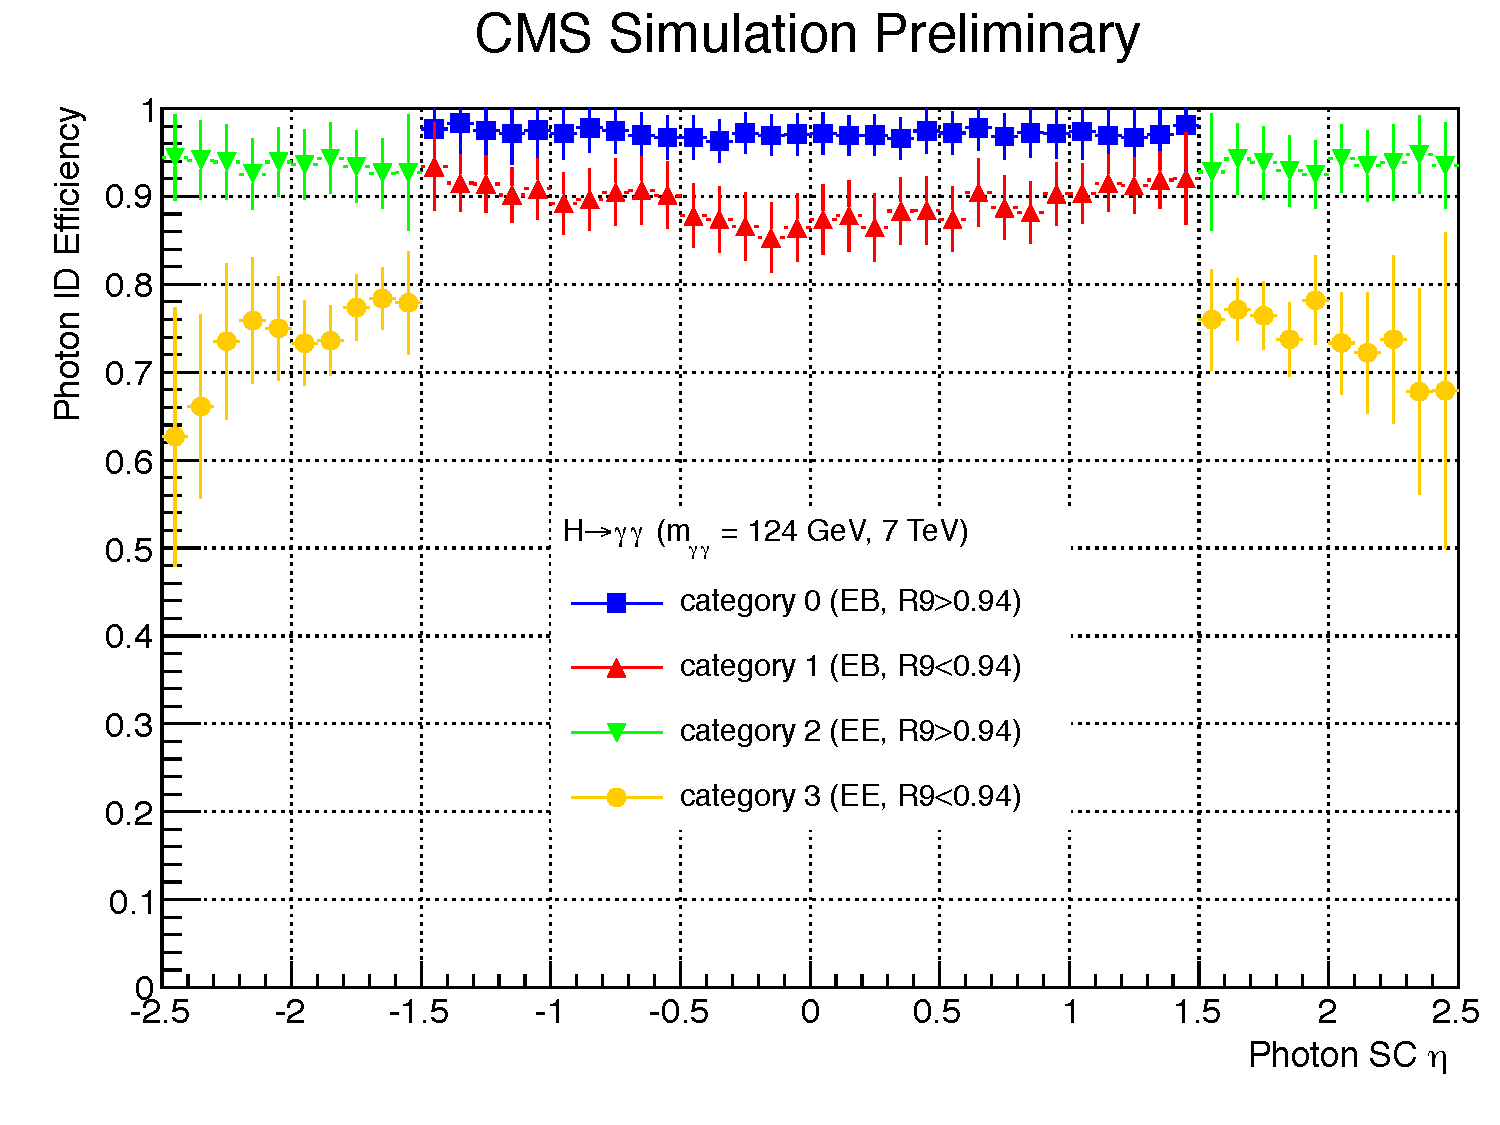
\includegraphics[width=0.49\textwidth]{selec_and_cats/plots/eff_7TeV_eta_fix.pdf}
  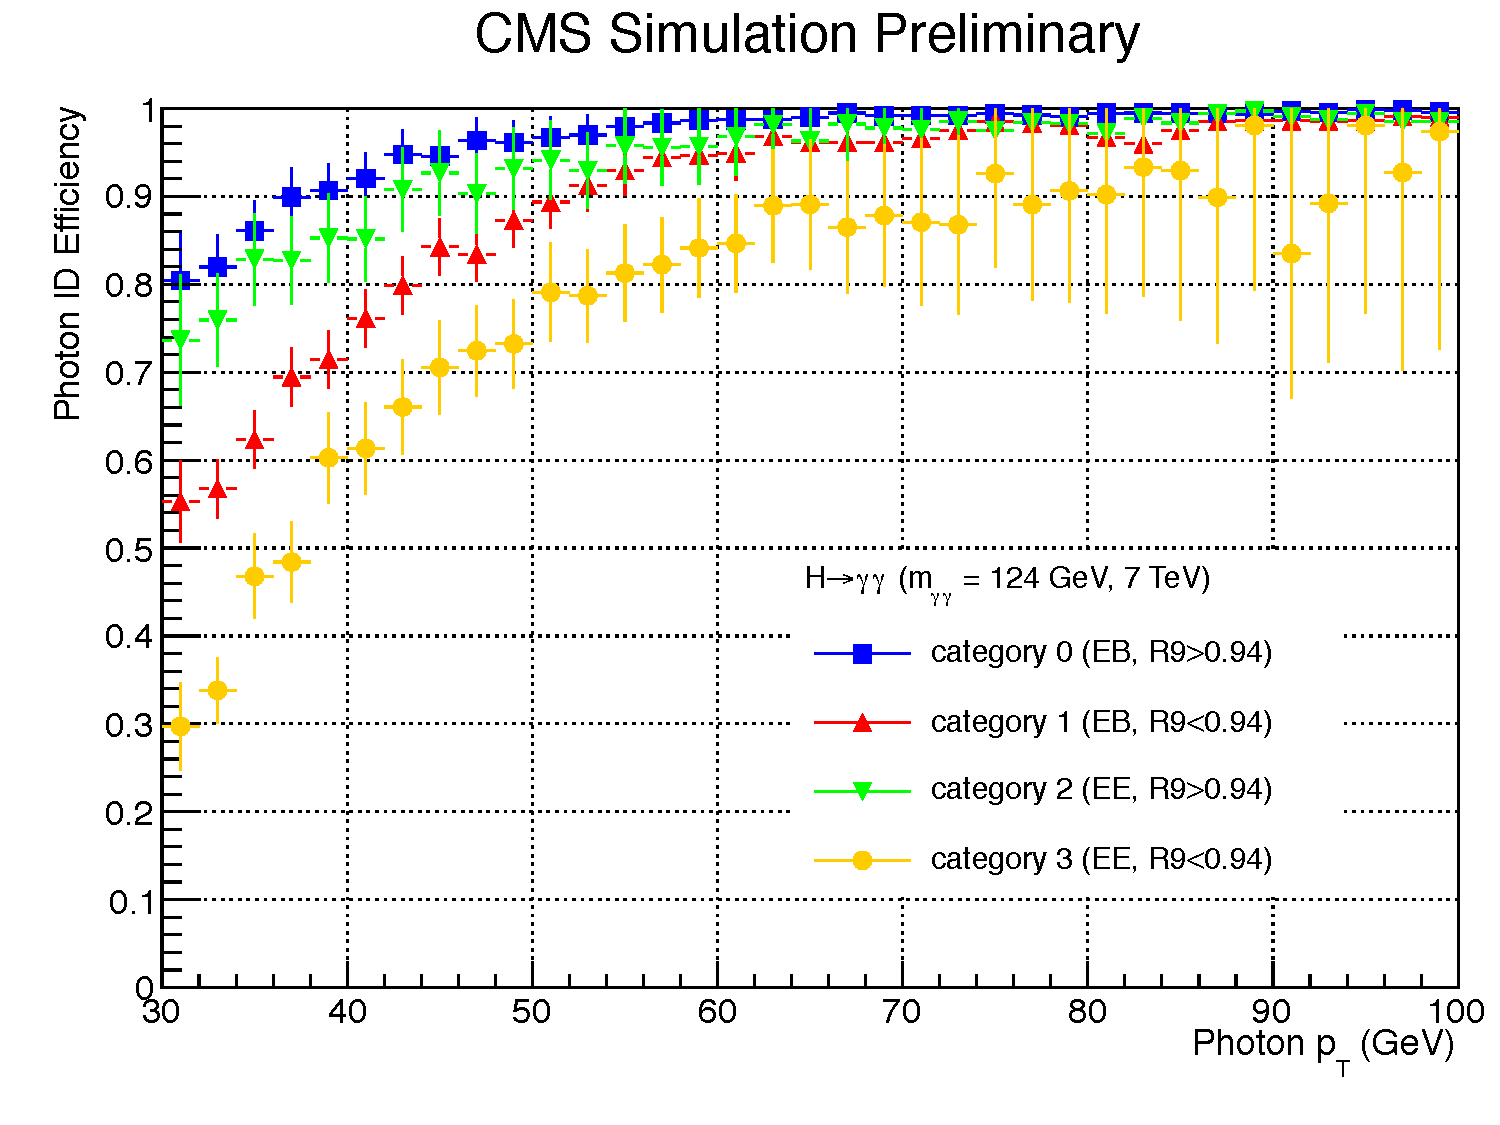
\includegraphics[width=0.49\textwidth]{selec_and_cats/plots/eff_7TeV_pt_fix.pdf}
  \includegraphics[width=0.49\textwidth]{selec_and_cats/plots/eff_8TeV_eta_fix.pdf}
  \includegraphics[width=0.49\textwidth]{selec_and_cats/plots/eff_8TeV_pt_fix.pdf}
  \caption[Cut based photon ID efficiency as measured in \Zee \acs{MC} simulation]{Cut based photon ID efficiency as measured in \Zee \MC simulation using the tag and probe method~\cite{tag_and_probe}. Shown for the 7~TeV dataset (top row) and 8~TeV dataset (bottom row) as a function of the photon supercluster position in \eta (left) and as a function of the photon \pT (right). Photons in the barrel which are unconverted (converted) are plotted as the blue (red) points and photons in the endcap which are unconverted (converted) are plotted as the green (yellow) points.}
  \label{fig:cic_efficiency}
\end{figure}

\subsection{Photon ID \acs{MVA}}
\label{sec:pho_id_mva}

For the \MFM and \SMVA analyses a \BDT is trained to discriminate between prompt photons and jets. The desire is to factorise the photon selection, which is required to distinguish prompt photons from neutral mesons faking photons, and the event selection, which is required to consider kinematics, resolution, etc.~to distinguish \Hgg from the $pp\rightarrow\gamma\gamma$, \gjet, $\mathrm{jet}+\mathrm{jet}$ background. The input variables used are designed specifically to distinguish between photons and fakes. They should not have any properties which make the identification Higgs specific. Consequently, the training samples used are \gjet samples where the identification \BDT signal is the prompt $\gamma$ and the background is the fake jet. The \pT and supercluster \eta distributions are reweighted such that they match between signal and background. This negates the \BDT exploiting any photon kinematics which could correlate to the Higgs mass. The photon ID \BDT is trained separately for the barrel and endcap as these regions of phase space are so different. Separate \BDTs were also trained for 7 and 8~TeV. The result is four separate trainings in total.

The input variables aim to exploit differences in the shower shape and isolation between prompt and non-prompt photons and the correlation between these variables and the supercluster position and energy. They are:

\noindent\textbf{Shower shape variables}
\begin{itemize}
  \item $\sigma_{i\eta i\eta}$ - Explained above in Sec.~\ref{sec:photon_presel}.
  \item $\sigma_{i\eta i\phi}$ - The equivalent diagonal spread (in \eta,\phi), representing the ($\eta$,$\phi$) correlation of the shower.
  \item $E_{2\times2}/E_{5\times5}$ - Ratio of the energy in the most energetic 2$\times$2 cluster which contains the seed to the energy in the 5$\times$5 cluster.
  \item $R_{9}$ - Explained above in Sec.~\ref{sec:ecal}.
  \item $\sigma_{\eta}$ - The energy-weighted standard deviation of single crystal \eta within the supercluster.
  \item $\sigma_{\phi}$ - The energy-weighted standard deviation of single crystal \phi within the supercluster.
  \item $\sigma_{xy}$ (for endcap only) - The standard deviation of the shower spread in the $x$, $y$ planes of the preshower, representing the $x$-$y$ correlation of the shower.
\end{itemize}

\noindent\textbf{Isolation variables}
\begin{itemize}
  \item PF Photon ISO - Particle flow photon isolation sum.
  \item PF Charged Hadron ISO (selected vertex) - Particle flow charged hadron isolation sum for candidates originating from selected vertex.
  \item PF Charged Hadron ISO (worst vertex) - Particle flow charged hadron isolation sum for candidates originating from the vertex with the largest isolation sum.
\end{itemize}

\noindent\textbf{Correlation variables}
\begin{itemize}
  \item $\rho$ - The median energy density in the event.
  \item $\eta$ - The \eta position of the photon supercluster.
  \item $E_{raw}$ - The raw energy of the photon supercluster.
\end{itemize}

The testing sample used to verify the output of the photon identification \BDT is a \MC \Hgg sample (\mH=124~\GeV). The photon identification \BDT output provides a measure of an individual photon's ``quality" and is used as an input to the event-level \BDT (described in the next section). Even so, a considerable amount of background is cut out by defining a loose cut (the \BDT output must be $>-0.2$) on the photon ID \BDT output value which is more than 99\% signal efficient. This is demonstrated in Fig.~\ref{fig:photon_id_bdt} which shows the photon ID \BDT output for a \Hgg signal \MC sample and for all the data events which pass the preselection defined in Sec.~\ref{sec:photon_presel}. It is clear that placing a cut at $>-0.2$ removes a considerable amount of the background whilst maintaining very high signal efficiency.

The photon ID \BDT response for each photon is used as a direct input to the event-level \MVA. Given that imperfect modeling of the detector response can result in a small change in the photon ID response, which has a direct impact on the event-level \MVA response, which is used to classify events, a systematic error on the photon quality is applied and propagated through to the event-level \MVA. Validation of the photon ID \BDT response in the \Zee decay is shown in Fig.~\ref{fig:photon_id_zee} with the size of the systematic error applied to account for any data/\MC discrepancies. The uniform response of the identification as a function of the number of primary vertices is demonstrated by the similarity of the two plots in this figure (Fig.~\ref{fig:photon_id_zee}) which are for events in which the number of primary vertices is $\leq 15$ (on the left) and for those in which the number of primary vertices is $>15$ (right).

\begin{figure}
  \includegraphics[width=0.48\textwidth]{selec_and_cats/plots/lowScoreID_7TeV_fix.pdf}
  \includegraphics[width=0.48\textwidth]{selec_and_cats/plots/lowScoreID_8TeV_fix.pdf}
  \caption[The output distribution of the photon identification \acs{BDT}]{The output distribution of the photon identification \BDT for 7~\TeV (left) and 8~\TeV (right) datasets. The black points show the output for data events which pass the preselection and the red histogram shows the output for a simulated \MC sample of \Hgg decays. A cut of $>-0.2$ is made on all photons.}
  \label{fig:photon_id_bdt}
\end{figure}

\begin{figure}
  \includegraphics[width=0.98\textwidth]{selec_and_cats/plots/idmva_nvtx_fix.pdf}
  \caption[The output distribution of the photon identification \acs{BDT} in \Zee decays]{The output distribution of the photon identification \BDT for the 8~\TeV training as validated by the \Zee decay for events which have $\leq15$ reconstructed primary vertices (left) and those which have $>15$ primary vertices (right). The data is shown as the black points with the \MC simulation as the blue histogram. The systematic uncertainty on the output as applied to the \MC sample is shown as the red band.}
  \label{fig:photon_id_zee}
\end{figure}

\subsection{Diphoton event-level \acs{MVA}}
\label{sec:diphoton_bdt}

Whilst the CiC analysis selects events based on photon identification, the \MVA analysis approach is to first select photons using the photon identification \BDT described in the section above and then pass all the relevant event information through an event-level \BDT. The event-level classifier, referred to as the diphoton \BDT, is constructed to give a high score to events which fulfill the following criteria:

\begin{enumerate}
  \item The event kinematics should be compatible with a Higgs decay.
  \item The event has good mass resolution.
  \item The event contains two ``high quality" photons (i.e.~they have a high score from the photon ID \BDT).
\end{enumerate}

It is highly important that the \BDT is completely independent of Higgs mass and consequently that the input variables have no, or at the least very little, dependence on the Higgs mass. This is essential to have a fair training. If the \BDT included the Higgs mass, or a variable highly correlated with it, it would preferentially select events with this mass therefore biasing the selection towards events which have a mass near the mass of the signal used to train with. The input variables used are:

\noindent\textbf{Event kinematics}
\begin{itemize}
  \item $p_{T}^{1(2)}/m_{\gamma\gamma}$ - The mass relative transverse momenta of each photon.
  \item $\eta^{1(2)}$ - The pseudorapidity of each photon.
  \item $\cos(\phi_{1}-\phi_{2})$ - The cosine of the angle between the two photons in the transverse plane. This variable reflects the \pT of the diphoton system (in other words the reconstructed Higgs candidate) without introducing a mass dependence.
\end{itemize}

\noindent\textbf{Mass resolution}
\begin{itemize}
  \item $\sigma_{m}^{right}/m_{\gamma\gamma}$ - The mass resolution of the event assuming the correct primary vertex has been selected. In this case the angular resolution is negligible so the variable is calculated using just the two photon energy resolution values as
    \begin{equation}
      \frac{\sigma_{m}^{right}}{m_{\gamma\gamma}} = \frac{1}{2}\Bigl(\frac{\sigma_{E_{1}}}{E_{1}} \oplus \frac{\sigma_{E_{2}}}{E_{2}}\Bigr).
    \end{equation}
  \item $\sigma_{m}^{wrong}/m_{\gamma\gamma}$ - The mass resolution of the event assuming the wrong vertex is selected. The vertex position in $z$ is distributed as a Gaussian with a width equivalent to $\sqrt{2}\sigma_{z}^{beamspot}$ and so the angular resolution $\sigma_{m}^{vtx}$ can be analytically calculated given the \ECAL impact positions of the two photons. Consequently the wrong vertex variable is calculated as
    \begin{equation}
      \frac{\sigma_{m}^{wrong}}{m_{\gamma\gamma}} = \frac{\sigma_{m}^{right}}{m_{\gamma\gamma}} \oplus \frac{\sigma_{m}^{vtx}}{m_{\gamma\gamma}}.
    \end{equation}
  \item $p_{vtx}$ - The probability that the selected primary vertex is correct. In order to tie together the mass resolution information given the right vertex hypothesis and the wrong vertex hypothesis, the probability that the vertex is correct is used in addition.
  \item It is also important to specify in the training that the signal to background ratio is inversely proportional to the mass resolution. Accordingly the signal events in the training are weighted by a factor,
    \begin{equation}
      w = \frac{p_{vtx}}{\sigma_{m}^{right}/m_{\gamma\gamma}} + \frac{1-p_{vtx}}{\sigma_{m}^{wrong}/m_{\gamma\gamma}}.
    \end{equation}
\end{itemize}

\noindent\textbf{Photon quality}
\begin{itemize}
  \item pho$ID^{1(2)}$ - The photon ID \BDT output value of each photon.
\end{itemize}

The training is performed separately for 7 and 8~\TeV and the samples used for the signal are all of the \SM \Hgg \MC samples (\ggH, \VBF, \VH, \ttH) appropriately weighted by cross section and the samples used for the background are the cross section-weighted mixture of \SM backgrounds which include contributions from $pp\rightarrow\gamma\gamma$ (prompt-prompt), $pp\rightarrow\gamma+\mathrm{jet}$ (prompt-fake) and $pp\rightarrow\mathrm{jet+jet}$ (fake-fake) as described in Sec.~\ref{sec:mc}. The training is performed on only half of each event sample (selected by even event number) so that the BDT response can be tested on the other half (selected by odd event number).

A cut is placed on the \BDT response in order to remove almost all of the events which contain two fake photons and a large fraction of those which contain one fake. The remaining events which pass this cut are those used in the results and get categorised in coarse bins based on the \BDT response. The strategy for optimising this cut value and the category boundaries is explained in Sec.~\ref{sec:categorisation}. The \BDT response in data, background and signal is shown in Fig.~\ref{fig:dipho_bdt}. The \BDT output in this figure has been transformed so that its response is flat for the total signal. This helps to see the differences between the signal (flat) and background (not flat) and also the differences between the gluon fusion signal and the other production modes. By examining the \BDT response in signal (top row of Fig.~\ref{fig:dipho_bdt}) one can see that the associated production modes (\VBF in yellow, \VH in green and \ttH in blue) peak closer to 1 relative to the gluon fusion signal (red). This is predominantly driven by the fact that Higgs bosons produced by associated modes are typically at higher \pT than for gluon fusion and this kinematic feature helps the \BDT to discriminate these events from the background. It can be seen in the bottom row of Fig.~\ref{fig:dipho_bdt} that the cut on the event-level \BDT removes a considerable amount of the fake-fake and prompt-fake contribution to the background with the remainder consisting of about 70\% prompt-prompt and 30\% prompt-fake.

\begin{figure}
  \includegraphics[width=0.475\textwidth]{selec_and_cats/plots/mixedbdt_transformed_7TeV_fix_fix.pdf} \hspace{0.05cm}
  \includegraphics[width=0.475\textwidth]{selec_and_cats/plots/mixedbdt_transformed_8TeV_fix_fix.pdf} \\
  \includegraphics[width=0.48\textwidth]{selec_and_cats/plots/diphobdt_transformed_bg_7TeV_fix_fix.pdf} \hspace{0.05cm}
  \includegraphics[width=0.48\textwidth]{selec_and_cats/plots/diphobdt_transformed_bg_8TeV_fix_fix.pdf}
  \caption[The diphoton \acs{BDT} response]{The diphoton \BDT response for the 7~\TeV training (left column) and 8~\TeV training (right column) transformed so that the output is flat in the signal. The top row shows the output in data (black points), which contains mostly background events, and signal \MC events (filled histograms) split by production mode; \ggH (red), \VBF (yellow), \VH (green), \ttH (blue). The bottom row shows the output in data (black points) and background \MC events (filled histograms) split by type; prompt-prompt (green), prompt-fake (yellow) and fake-fake (red). The data/background residual is shown as the blue points underneath these histograms. The vertical dashed lines show the analysis category definitions where those on the right (nearer a classifier score of 1) have the highest S/B ratio. All events which fall below the left most boundary, shown by the shaded area, are cut out of the analysis.}
  \label{fig:dipho_bdt}
\end{figure}

Any uncertainties which affect the shape of the output distribution of this \BDT result in event migrations between the final analysis categories; if the \BDT response is mismodelled then events can move across the boundaries represented as the vertical dashed lines in Fig.~\ref{fig:dipho_bdt}. The signal model in this analysis is obtained from \MC simulation and so these uncertainties can have an effect on the signal model shape in each of the categories. Whilst these migrations may also be true of the background the effect is not important because the background is extracted from data. The input variables whose uncertainties have the largest effect on the \BDT response in signal are the photon ID quality and the photon energy resolution estimate. This is because these variables have both i) relatively large uncertainties because of imperfect detector response modelling in the simulation and ii) are highly discriminative and hence can have a relatively large impact on the \BDT response. As the \BDT response varies monotonically with these variables, the systematic uncertainty on them is propagated through the analysis as an event migration. Systematic uncertainties are described in more detail in Sec.~\ref{sec:systematics}. The size of this effect is shown in the \BDT response validation plot using the \Zee decay in Fig.~\ref{fig:diphotonBDT_zee}.

\begin{figure}
  \includegraphics[width=0.95\textwidth]{selec_and_cats/plots/transformedBDT_single_syst_fix_fix.pdf}
  \caption[The diphoton \acs{BDT} response in \Zee decays]{The diphoton BDT response for the 8~\TeV training in the \Zee decay. The data is shown as the black points and the \MC events as the blue histogram. The systematic applied to account for variation in the BDT response from mismodelling in the photon quality response and the photon energy resolution estimate are shown as the red band. The vertical dashed lines show the boundaries of the analysis categories.}
  \label{fig:diphotonBDT_zee}
\end{figure}

% ---- SECTION ----
\section{Event categorisation}
\label{sec:categorisation}

In order to exploit different regions of phase space with dissimilar signal to background ratios the events are split into categories. Furthermore, additional categories can be designed to enrich the selection with events characteristic of particular Higgs production modes. The \VBF production mode is typically accompanied by a pair of jets with a large pseudorapidity separation. The \VH production, which includes contributions from \WH and \ZH, may be accompanied by a charged lepton, missing transverse energy or jets originating from the decay of the associated $W$ or $Z$ boson. Similarly, \ttH production may be accompanied by $b$ quarks and/or charged leptons. The predominant production mode, which accounts for about 88\% of the signal, is \ggH and is inclusive. The amount of signal produced from exclusive modes is approximately 8\% for \VBF, 4\% for \VH and $<$1\% for \ttH. By including a series of event tags, and separating events accordingly, all four production modes of the Higgs at the \LHC are harnessed in this analysis. This not only helps to increase the overall sensitivity to a \SM Higgs boson (given the very low background rates expected for the exclusive modes) but also significantly helps to reduce the error on measurements of the relative couplings of the observed boson to fermions and bosons, as the signal from the relative production modes gets split into distinct categories. This ``exclusive mode tagging" is done identically for both the nominal \MFM analysis and also the cross-check \SMVA, although the inclusive mode categorisation is done differently. The \CiC spin analysis uses no exclusive mode tagging as the spin-2 models considered (minimal coupling graviton) have only inclusive production modes. There is an alternate categorisation scheme used for the spin analysis which exploits both the event mass resolution and the differential decay angle.

\subsection{Exclusive mode tagging}
\label{sec:exclusive_tags}
All events which make it to this stage will have passed the photon preselection (Sec.~\ref{sec:photon_presel}), as well as the basic requirement of two high \pT photons with $100<m_{\gamma\gamma}<180$~GeV (Sec.~\ref{sec:event_selection}) and the \MFM analysis selection (Sec.~\ref{sec:diphoton_bdt}), which includes both the photon ID \MVA cut and the diphoton event-level \BDT cut. These make up the final event sample. They now pass through the ``tagging" procedure described below in which they are organised into a set of non-overlapping event classes. The tagging is done in a specific order to ensure there is no overlap between classes and the order is chosen such that preference is given to categories with a higher expected signal to background ratio. The aim of the exclusive mode tagging is to seperate events into their most probable production mode (one of \VBF, \VH or \ttH) where the events which are left ``Untagged" are mostly produced by \ggH. The tagging order is shown alongside a summary of the relevant cut values in Table~\ref{tab:cat_summary} at the end of the chapter. If an event does not meet the requirements of a particular tag it is passed onto the next tag and if it fails all tag requirements it is placed in one of the inclusive categories, whose structure is described below (Secs.~\ref{sec:inclusive_cats_massfac}-\ref{sec:inclusive_cats_sideband}), meaning that no event cannot be included in the analysis.

\subsubsection{Dijet-tagged categories for VBF}
\label{sec:vbf_tag}

The following variables are used to exploit the specific topology of the jet pairs associated to \VBF Higgs production:

\begin{itemize}
  \item $p_{T}^{\gamma}/m_{\gamma\gamma}$ - The transverse momenta of the leading and subleading photons as a ratio of the diphoton invariant mass.
  \item $p_{T}^{\mathrm{j}}/m_{\gamma\gamma}$ - The transverse momenta of the leading and subleading jets as a ratio of the diphoton invariant mass.
  \item $m_{\mathrm{jj}}$ - The dijet invariant mass.
  \item $|\Delta\eta_{\mathrm{j}_{1}\mathrm{j}_{2}}|$ - The absolute pseudorapidity difference between the two jets.
  \item $Z = \eta(\gamma_{1})+\eta(\gamma_{2}) - \bigl[\eta(\mathrm{j}_{1})+\eta(\mathrm{j}_{2})\bigr]/2$ - The so-called \emph{Zeppenfeld} variable~\cite{Zeppenfeld}.
  \item $\Delta\phi_{\mathrm{j}_{1}\mathrm{j}_{2}}$ - The angular difference between the two jets in the transverse plane.
\end{itemize}

Additionally the leading photon \pT requirement is raised to $p_{T}^{\gamma_{1}}/m_{\gamma\gamma}>1/2$. The energy measurement of jets in the event are calibrated to correct for detector effects~\cite{jet_energy_corrections} and additional energy in the jets from pileup is removed using the \textsc{FastJet} jet areas technique described in~\cite{pu_jets1,pu_jets2,pu_jets3}. Jets are required to be within the pseudorapidity range $|\eta|<4.7$.

The dijet tagging is done with use of two additional \MVAs. The first is designed to exploit the \VBF kinematic properties and the second is used to combine this information with the diphoton \BDT. Candidates are required to pass a \VBF preselection of two jets with $p_{T}^{\j_{1}}>30$~\GeV and $p_{T}^{\j_{2}}>20$~\GeV and invariant mass, \mjj$>75$~\GeV. The signal sample used for training is the \SM \MC simulation with just \VBF production, whilst the \SM gluon fusion \MC simulation is included as background along with the usual prompt-prompt, prompt-fake and fake-fake contributions. This helps produce an output in which a high score gives a very pure \VBF sample.

The combined dijet-diphoton \BDT has inputs of the kinematic dijet \BDT output, the diphoton \BDT output and $p_{T}^{\gamma\gamma}/m_{\gamma\gamma}$ in order to discriminate \VBF from both the other signal types and the background, utilising all the information available in the event. The transverse momenta of the diphoton system as a ratio of the diphoton invariant mass, $p_{T}^{\gamma\gamma}/m_{\gamma\gamma}$, is included both because of its discriminating power and the differences between signal and background of its correlation with both the dijet \BDT output and the diphoton \BDT output.

One finds that the background rejection for \VBF is significantly improved by the use of the combined dijet-diphoton \BDT whilst the \VBF purity (i.e.~separation from \ggH) is not as good when collapsing the kinematic dijet \BDT and the combined \BDT into one step. Consequently the trainings are performed separately and the \VBF categories are defined by picking out regions which have a high score in the combined dijet-diphoton \BDT response. Each successive \BDT training uses statistically independent \MC samples to avoid selection bias from fluctuations in the simulation. The optimisation procedure for deciding the category boundaries is analogous to the one used for the inclusive categories in the \MFM analysis where the target is to minimise the expected uncertainty of the signal strength from the \VBF process alone when moving the boundaries around. The optimisation procedure includes the statistical disadvantage of having too many categories for a given dataset size. This is explained further in Section~\ref{sec:inclusive_cats_massfac}. At 8~\TeV there are three \VBF categories and at 7~\TeV there are two, because of the considerably lower statistics in the 7~TeV dataset. The output distributions at 7 and 8~TeV for the signal are shown for the kinematic dijet \BDT in Fig.~\ref{fig:vbf_dijet_kin} and for the combined diphoton-dijet \BDT, along with the \VBF category boundaries, in Fig.~\ref{fig:vbf_dijet_comb}. The \BDT response shown in these plots is transformed so that it is flat in the \VBF signal (yellow histogram). One can see that the other signal types peak lower in the transformed score and the data, which contains mostly background, even more so.

\begin{figure}
  \includegraphics[width=0.48\textwidth]{selec_and_cats/plots/dijetbdt_transformed_signal_7TeV_fix_fix.pdf}
  \includegraphics[width=0.48\textwidth]{selec_and_cats/plots/dijetbdt_transformed_signal_8TeV_fix_fix.pdf}
  \caption[The kinematic dijet \acs{BDT} response]{The distributions of the kinematic dijet \BDT response at 7~TeV (left) and 8~TeV (right) for the signal split by production mode; \ggH (red), \VBF (yellow), \VH (green) and \ttH (blue). The output is transformed so that it is flat in the \VBF signal.}
  \label{fig:vbf_dijet_kin}
\end{figure}

\begin{figure}
  \includegraphics[width=0.48\textwidth]{selec_and_cats/plots/mixedcombbdt_transformed_7TeV_fix_fix.pdf}
  \includegraphics[width=0.48\textwidth]{selec_and_cats/plots/mixedcombbdt_transformed_8TeV_fix_fix.pdf}
  \caption[The distribution of the combined dijet-diphoton \acs{BDT} response]{The distributions of the combined dijet-diphoton \BDT response at 7~TeV (left) and 8~TeV (right) for the data (black points), which contains mostly background, and signal (filled histograms) split by production mode; \ggH (red), \VBF (yellow), \VH (green) and \ttH (blue). The output is transformed so that it is flat in the \VBF signal. The vertical dashed lines show the \VBF category definitions where those on the right (nearer a classifier score of 1) are purest \VBF signal. All events which fall below the left most boundary are not included in \VBF categories but fall back to being categorised amongst the inclusive categories.}
  \label{fig:vbf_dijet_comb}
\end{figure}

\subsubsection{Lepton-, jet- and \MET-tagged categories for \VH}
\label{sec:vh_tag}

The selection for the four categories designed to tag \VH production are optimised by minimising the expected uncertainty on the signal strength of this process alone. Two of the classes require at least one charged muon or electron and are split into a tight selection category and a looser selection category, the third is for events consistent with large \MET and the fourth for events consistent with two or more jets. The leading photon cut is raised to $p_{T}^{\gamma_{1}}/m_{\gamma\gamma}>3/8$ for all \VH-tagged categories. The category requirements are as follows:

\begin{itemize}
  \item \textbf{\VH Tight $l$}: The tightly selected lepton category is characterised by the signature of a leptonically decaying $W$ or $Z$ boson and as such requires the presence of \MET$>35$~\GeV or another lepton of the same flavour and opposite charge as the first. In the first case (of a lepton + \MET) the lepton is required to have $p_{T}>20$~\GeV, in the latter case (of two leptons) the requirement is $p_{T}>10$~\GeV for both leptons whilst the invariant mass of the dilepton pair must be $70 < m_{ll} < 110$~\GeV. The diphoton \BDT output is required to be $>0.1$ ($>-0.6$) for the 7 (8)~\TeV datasets.
  \item \textbf{\VH Loose $l$}: For the loosely selected lepton category the lepton \pT must satisfy $p_{T}>20$~\GeV. The selection requirements are designed to reduce the background from leptonic $Z$ bosons (not associated with a Higgs) that contain initial or final state radiation faking the diphoton signal. Consequently, leptons are required to be separated by at least $\Delta R>1.0$ from the closest photon and the invariant mass of any lepton-photon pairs must be more than 10~\GeV away from the $Z$ boson mass. In addition a conversion veto is applied to the electrons to reduce the rate of misidentified photons. The diphoton \BDT output is required to be $>0.1$ ($>-0.6$) for the 7 (8)~\TeV datasets.
  \item \textbf{\VH \MET tag}: Accurate measurement and simulation of the \MET vector has been studied in detail at \CMS and a set of standard corrections (for both data and simulation) are applied~\cite{met_corrs}. The corrected \MET is required to pass \MET$>70$~\GeV whilst the angular separation in the transverse plane between the momentum of the diphoton system and the \MET direction must pass $\Delta\phi(\gamma\gamma,\MET)>2.1$, and similarly the angle between the momentum of the diphoton system and the leading jet must pass $\Delta\phi(\gamma\gamma,\mbox{jet})<2.7$. The diphoton \BDT output is required to be $>0.8$ ($>0.0$) for the 7 (8)~\TeV datasets.
  \item \textbf{\VH dijet tag}: The event must contain at least one jet pair in which both jets have $p_{T}>40$~\GeV and $|\eta|<2.4$ and have an invariant mass within the range $60<m_{jj}<120$~\GeV. The diphoton transverse momentum must satisfy $p_{T}^{\gamma\gamma}/m_{\gamma\gamma}>13/12$. Additionally the angular correlation between the diphoton system and the dijet system from \VH-associated Higgs decays can be exploited. The angle, $\theta^{\star}$, between the diphoton direction in the diphoton-dijet rest frame and the lab frame is flat for events from \VH decays whereas for the background and gluon fusion-produced Higgs decays the distribution peaks at $|\cos(\theta^{\star})|=1$. Consequently, there is a requirement that $|\cos(\theta^{\star})|<0.5$. The diphoton \BDT output is required to be $>0.6$ ($>0.2$) for the 7 (8)~\TeV datasets.
\end{itemize}

\subsubsection{Lepton- and jet-tagged categories for \ttH}
\label{sec:tth_tag}

There are two categories for tagging production from \ttH decays, one of which is lepton-based and one of which is jet-based. The total fraction of signal expected from \ttH is $<$1\% so only a handful of events are expected. Consequently for the 7~\TeV dataset the two categories are merged into one class. As for the \VH-tagged categories, the cuts are optimised to minimise the expected uncertainty of the signal strength measurement of the \ttH process alone.

For both classes the leading photon \pT cut is raised to $p_{T}^{\gamma_{1}}/m_{\gamma\gamma}>1/2$, all jets are required to have \pT$>25$~\GeV and there must be at least one b-tagged jet present. The specific requirements of each category are as follows:

\begin{itemize}
  \item \textbf{\ttH multijet tag}: The requirement is at least four additional jets in the event and no lepton. The diphoton \BDT output is required to be $>0.6$ ($>-0.2$) for the 7 (8)~\TeV datasets.
  \item \textbf{\ttH lepton tag}: At least one more jet in the event and one muon or electron which has \pT$>20$~\GeV. The diphoton \BDT output is required to be $>0.6$ ($>-0.6$) for the 7 (8)~\TeV datasets.
\end{itemize}

%\subsection{Inclusive mode categorisation in the cut based analysis}
%\label{sec:inclusive_cats_cic}

%Any event which passes the cut based photon selection described in Section~\ref{sec:cic} and does not fall into one of the exclusive categories described above is split into one of eight inclusive categories depending on the supercluster position, \eta, of the two photons, the conversion variable, \rnine, of the two photons and the mass relative diphoton transverse momenta, \pToM. The categories are defined in Table~\ref{tab:cic_cats}.

%\begin{table}
%  \begin{center}
%    \begin{tabular}{lccc}
%                 & \pToM                            & Maximum \eta                                    & Minimum \rnine \\
%      \hline
%      Untagged 0 & \multirow{4}{*}{$>40$~\GeV}      & \multirow{2}{*}{$<$1.444}                       & $>0.94$ \\
%      Untagged 1 &                                  &                                                 & $<0.94$ \\
%      Untagged 2 &                                  & \multirow{2}{*}{$<$2.5}                         & $>0.94$ \\
%      Untagged 3 &                                  &                                                 & $<0.94$ \\
%      \hline
%      Untagged 4 & \multirow{4}{*}{$<40$~\GeV}      & \multirow{2}{*}{$<$1.444}                       & $>0.94$ \\
%      Untagged 5 &                                  &                                                 & $<0.94$ \\
%      Untagged 6 &                                  & \multirow{2}{*}{$<$2.5}                         & $>0.94$ \\
%      Untagged 7 &                                  &                                                 & $<0.94$ \\
%    \end{tabular}
%    \caption{The definition of the inclusive categories for the \CiC analysis}
%    \label{tab:cic_cats}
%  \end{center}
%\end{table}

\subsection{Inclusive mode categorisation and VBF dijet categorisation in the mass-factorised \acs{MVA} analysis}
\label{sec:inclusive_cats_massfac}

The combined dijet-diphoton \BDT output value is used to define a set of \VBF categories. The goal is to find the configuration of category boundaries which minimise the expected uncertainty on the signal strength for \VBF production alone, allowing the number of categories and where the category boundaries lie to be completely free floating, with the additional requirement that the efficiency $\times$ acceptance of the categories matches between 7 and 8~\TeV. This results in a tight \VBF category for events with a very high combined dijet-diphoton \BDT score, a somewhat looser category and then one or more very loose categories. It is found that dropping the loosest category has a negligible impact ($<$1\%) on the expected uncertainty and as such the upper boundary for the loosest category is turned into a lower cut. All events which pass the \VBF preselection (described in Sec.~\ref{sec:vbf_tag}) and fail the lower cut are then classified somewhere in the inclusive categories defined below.

Once the \VBF category boundaries have been found the same procedure is deployed using the diphoton \BDT output value. This time the target is to minimise the expected uncertainty on the total signal strength, allowing the number of categories and the category boundary values to be completely free floating. One finds a rather similar structure and that dropping events in the very loosest category has a negligible impact on the performance and consequently this dictates the lower cut value for the diphoton \BDT. The expected uncertainty minima, when floating both the number of category boundaries and the boundary locations, are fairly shallow so the exact position of the boundaries has a very small impact on the performance of the analysis. For the 7 (8)~\TeV datasets there are 4 (5) inclusive categories with a lower diphoton \BDT cut of 0.19 ($-0.78$) and 2 (3) \VBF categories\footnote{There are fewer categories in the 7~TeV dataset because there are less statistics.}.

\subsection{Inclusive mode categorisation in the sideband \acs{MVA} analysis}
\label{sec:inclusive_cats_sideband}

In the \SMVA analysis all the exclusive categories are identical to the \MFM analysis (including the \VBF categories). However the inclusive categorisation is done slightly differently. In the sideband analysis the signal region is defined in a $\pm2$\% window around the hypothesis Higgs mass and thus contains $\sim75\%$ of the signal. The analysis is performed as a cut and count in the signal window over several bins. There is one bin for each exclusive category and then several more for the inclusive. The binning scheme for the inclusive events is defined as follows,

\begin{itemize}
  \item Make two-dimensional distributions of the diphoton \BDT score and the distance of the invariant mass from the hypothesised Higgs mass, $\Delta m/m_{H}$, in the $\pm2$\% window for signal and background, as shown in Figure~\ref{fig:sideband_inputs}, where,
    \begin{equation}
      \frac{\Delta m}{m_{H}} = \frac{m_{\gamma\gamma} - m_{H}}{m_{H}}.
    \end{equation}
  \item Use a local regression smoothing technique~\cite{regression_smoothing} to smooth statistical fluctuations within the sample (demonstrated in Fig.~\ref{fig:sideband_inputs}).
  \item Select bins by isolating regions of this 2D phase space which have similar $S/B$ ratios and optimise the boundaries to give the maximum expected signal significance.
\end{itemize}

Clearly the most sensitive bins will be the ones which have a high diphoton \BDT score and have a low value of $|\dmom|$ (i.e.\ are near the signal peak). The category boundaries in this 2D plane are shown as different shades in Figure~\ref{fig:sideband_cats}. In total there are 8 (10) inclusive bins for the 7 (8)~\TeV samples in the \SMVA. There are some small residual differences between the raw \MC distributions and the smoothed distributions, shown in Fig.~\ref{fig:sideband_inputs}, especially near the high side boundary where smoothing algorithms can have difficulties. However, it has been found that artificially resolving such discrepancies results in a small change to the position of the category boundaries and furthermore that small changes in the boundary definitions have a very small impact on the sensitivity of the analysis. It should be noted that changing the location of the category boundaries cannot bias the result but only provide a non-optimal result. Consequently such discrepancies are considered unimportant as they do not influence the central value of the result and are only estimated to decrease the sensitivty by $<2\%$.

\begin{figure}
  \includegraphics[width=0.48\textwidth]{selec_and_cats/plots/sideband_bkg_7TeV_fix.pdf}
  \includegraphics[width=0.48\textwidth]{selec_and_cats/plots/sideband_sig_7TeV_fix.pdf} \\
  \includegraphics[width=0.48\textwidth]{selec_and_cats/plots/sideband_diphobdt_7TeV_fix.pdf}
  \includegraphics[width=0.48\textwidth]{selec_and_cats/plots/sideband_dmom_7TeV_fix.pdf} \\
  \caption[Two dimensional distributions of the diphoton \acs{BDT} output and \dmom for the sideband analysis]{Two dimensional distributions of the diphoton \BDT output and \dmom are shown on the top row for the background (left) and signal (right) for the 7~\TeV sample. The bottom rows shows the projections for signal (red) and background (blue) in the two variables.}
  \label{fig:sideband_inputs}
\end{figure}

\begin{figure}
  \includegraphics[width=0.48\textwidth]{selec_and_cats/plots/sideband_cats_7TeV_fix.pdf}
  \includegraphics[width=0.48\textwidth]{selec_and_cats/plots/sideband_cats_8TeV_fix.pdf}
  \caption[The inclusive category bin definitions for the \acs{SMVA} analysis]{The inclusive category bin definitions for the \SMVA analysis. Shown for the 7~\TeV dataset on the left and the 8~\TeV dataset on the right.}
  \label{fig:sideband_cats}
\end{figure}

\subsection{Inclusive mode categorisation in the spin analysis}
\label{sec:spin_cats}

The Landau-Yang theorem forbids the direct decay of a spin-1 particle into a pair of photons~\cite{Landau1948,Yang1950}.
Consequently the spin analysis compares the expectation of the spin-0 SM Higgs, $J^{P}=\zerop$, and the spin-2 \emph{graviton-like}
model with minimal couplings, \twomp,~\cite{Gao2010}. The \twomp graviton resonance is produced in one of two ways, gluon-fusion ($gg$)
or quark-antiquark annihilation (\qqbar). As the \twomp is just one of many spin-2 models it is desirable to make the analysis as model-independent as possible. As a means of
discriminating between the two hypotheses, use is made of the scattering angle in the Collins-Sopper frame, \costhetastar ~\cite{CollinsSoper1977}, which is defined as the angle, in the diphoton rest frame, between the collinear diphotons
and the line which bisects one incoming beam with the negative of the other beam,
\begin{equation}
  \cos(\theta^{\ast}_{\mbox{\tiny{CS}}}) = 2\times\frac{E_{2}p_{z1}-E_{1}p_{z2}}{m_{\gamma\gamma}\sqrt{m^{2}_{\gamma\gamma}+p^{2}_{T\gamma\gamma}}},
  \label{eq:costheta}
\end{equation}
where $E_{1}$ and $E_{2}$ are the energies of the leading and trailing photon, $p_{z1}$ and $p_{z2}$ are the $z$-component momenta
of the leading and trailing photon and $m_{\gamma\gamma}$ and $p_{T\gamma\gamma}$ are the invariant mass and transverse momenta of the diphoton system.

In the diphoton rest frame the photons from the decay of a spin-0 boson are isotropic. Hence prior to acceptance cuts, the distribution of \costhetastar
under the \zerop hypothesis is uniformly flat. In general this is not the case for spin-2 decays.

In order to reduce any model dependence in the analysis the cut-based photon selection, described in Sec.~\ref{sec:cic}, is used to pick events by applying the cuts to both the leading and subleading photon candidates. The \MVA methods used for event selection in the nominal analysis use specific \SM \MC training samples and most importantly one of the training variables used, namely $\cos(\phi_{1}-\phi_{2})$, is highly correlated to the angular variable, \costhetastar, which can be used to distinguish spin hypotheses. Furthermore, given the unusual production modes of a spin-2 boson, no exclusive tagging is used in the spin analysis. The impact of using jet variables was studied but it was found that the sensitivity for distinguishing spin hypotheses was improved by a negligible amount.

The effect of the photon selection cuts on the distributions of
\abscostheta is illustrated in Fig.~\ref{fig:acc_cuts}. Before any acceptance cuts, Fig.~\ref{fig:acc_cuts} (left), the \abscostheta
distribution of the \zerop processes is flat. This is not the case for the \twomp processes (gluon-fusion and quark-antiquark annihilation). After the selection cuts are applied these distributions are considerably distorted, Fig.~\ref{fig:acc_cuts} (right). As a Higgs produced from vector boson-fusion, which is $\sim$8\% of the total (compared to $\sim$88\% from gluon fusion),  is typically produced at higher transverse momentum there is some additional contribution of \zerop signal at high values of \abscostheta compared to the \twomp production modes after the selection cuts.

\begin{figure}
	\begin{center}
	\includegraphics[width=0.49\linewidth]{analysis/plots/spin/before_7TeV.pdf}
	\includegraphics[width=0.49\linewidth]{analysis/plots/spin/after_7TeV.pdf} \\
	\includegraphics[width=0.49\linewidth]{analysis/plots/spin/before_8TeV.pdf}
	\includegraphics[width=0.49\linewidth]{analysis/plots/spin/after_8TeV.pdf} \\
	\caption[The distribution of \abscostheta before and after selection cuts for different spin signals]{The distribution of \abscostheta before any selection cuts (left) and after the selection cuts (right) for the 7~\TeV dataset (top row) and the 8~\TeV dataset (bottom row). The three histograms represent the spin $0^+$ distribution with all SM production modes (red circular points), the spin $2^+_m$ distribution with the gluon-fusion production mode (blue square points) and the spin $2^+_m$ distribution with the quark-antiquark annihilation production mode (green triangular points). The \abscostheta category boundaries are shown as the black dashed lines.}
	\label{fig:acc_cuts}
	\end{center}
\end{figure}

A robust analysis is possible because although the acceptance $\times$ efficiency varies considerably as a function of \abscostheta, the shape of this variation is largely independent of the spin-parity model. This is also true in restricted ranges of $\eta$ and $R_{9}$ which allows us to extract the signal yield in bins of \abscostheta in a comparatively model-independent way.
Figure~\ref{fig:eff_acc} shows the efficiency $\times$ acceptance ratio between the \twomp (with gluon-fusion production only) and \zerop (all SM production modes) as a function of \abscostheta in the $|\eta|$ and $R_{9}$ categories defined in Table~\ref{table:cats1}. It is clear that the acceptance $\times$ efficiency between the spin-0 and spin-2 models is independent of \abscostheta apart from at high values of \abscostheta where the vector boson-fusion production in the SM plays a role. This motivates the choice of \abscostheta category boundaries described below where all the categories have similar efficiency $\times$ acceptance apart from the bin highest in \abscostheta.

\begin{figure}
	\begin{center}
	\includegraphics[width=0.49\linewidth]{analysis/plots/spin/effacccats_7TeV.pdf}
	\includegraphics[width=0.49\linewidth]{analysis/plots/spin/effacccats_8TeV.pdf}
  \caption[Acceptance $\times$ efficiency ratio between the \twomp (gluon fusion production) and \zerop (all SM production modes) of the spin analysis event selection]{Acceptance $\times$ efficiency ratio between the \twomp (gluon-fusion production) and \zerop (all SM production modes) of the event selection as a function of \abscostheta split into the $|\eta|$ and $R_{9}$ categories defined in Table~\ref{table:cats1}. The \abscostheta category boundaries are shown as the black dashed lines. The left hand plot is for the 7~\TeV and the right hand plot for the 8~\TeV.}
	\label{fig:eff_acc}
	\end{center}
\end{figure}

To benefit from the improved energy resolution of non-showering photons in
the barrel, each event is categorised in $\eta$ and $R_{9}$ according to Table~\ref{table:cats1}.

\begin{table}
  \begin{center}
    \caption[Definition of the photon resolution categories in the spin analysis]{Definition of the photon resolution categories in the spin analysis. Here $|\eta|_{\mbox{\tiny{max}}}$ and $R_{9\mbox{\tiny{min}}}$ refer to the maximum $\eta$ and minimum $R_{9}$ of the two photons.}
    \begin{tabular}{ l | l l l }
      Category 0 & $|\eta|_{\mbox{\tiny{max}}}<1.444$ & and & $R_{9\mbox{\tiny{min}}}\geq0.94$ \tabularnewline
      Category 1 & $|\eta|_{\mbox{\tiny{max}}}<1.444$ & and & $R_{9\mbox{\tiny{min}}}<0.94$ \tabularnewline
      Category 2 & $|\eta|_{\mbox{\tiny{max}}}>1.556$ & and & $R_{9\mbox{\tiny{min}}}\geq0.94$ \tabularnewline
      Category 3 & $|\eta|_{\mbox{\tiny{max}}}>1.556$ & and & $R_{9\mbox{\tiny{min}}}<0.94$ \tabularnewline
    \end{tabular}
    \label{table:cats1}
  \end{center}
\end{table}

%\begin{tabular}{l l l l l}
%  \textbullet & Category 0: & $|\eta|_{\mbox{\tiny{max}}}<1.444$ & and & $R_{9\mbox{\tiny{min}}}>0.94$ \\
%  \textbullet & Category 1: & $|\eta|_{\mbox{\tiny{max}}}<1.444$ & and & $R_{9\mbox{\tiny{min}}}\leq0.94$ \\
%  \textbullet & Category 2: & $|\eta|_{\mbox{\tiny{max}}}>1.444$ & and & $R_{9\mbox{\tiny{min}}}>0.94$ \\
%  \textbullet & Category 3: & $|\eta|_{\mbox{\tiny{max}}}>1.444$ & and & $R_{9\mbox{\tiny{min}}}\leq0.94$ \\
%\end{tabular}

Within each category events are binned in \abscostheta, to discriminate between the different spin hypotheses, according to Table.~\ref{table:cats2}.

\begin{table}
  \begin{center}
    \caption[Definition of diphoton \abscostheta categories in the spin analysis]{Definition of diphoton \abscostheta categories in the spin analysis.}
    \begin{tabular}{ l | r l }
      Spin Category 0 &             & \abscostheta $<0.2$ \tabularnewline
      Spin Category 1 & $0.2\leq$   & \abscostheta$<0.375$ \tabularnewline
      Spin Category 2 & $0.375\leq$ & \abscostheta$<0.55$ \tabularnewline
      Spin Category 3 & $0.55\leq$  & \abscostheta$<0.75$ \tabularnewline
      Spin Category 4 & $0.75\leq$  & \abscostheta$<1.0$ \tabularnewline
    \end{tabular}
    \label{table:cats2}
  \end{center}
\end{table}

The \abscostheta boundaries are optimised to make particular use of the most discriminating
bin (high \abscostheta) and to maintain uniform acceptance $\times$ efficiency in the
other bins. In total the analysis is split into 20 event classes (4 $\eta$/\rnine\xspace
categories $\times$ 5 \abscostheta categories) in each year which gives a total of 40 event classes.

\subsection{Event categorisation summary}

All the categories and the tagging order are summarised in Table~\ref{tab:cat_summary}.

\begin{table}[h!]
\caption[The event classes at 7 and 8~TeV and some of their main selection requirements]{The event classes at 7 and 8~\TeV and some of their main selection requirements. Events are tested against the selection requirements
of the classes in the order they are listed here. A breakdown of the amount of signal, background and data in each category is shown in Fig.~\ref{fig:signal_composition}.}
\begin{center}
\begin{tabular}{l c c p{10cm}}
\multirow{2}{*}{Label} & \multicolumn{2}{l}{No. of classes} & \multirow{2}{*}{Main requirements} \\
 & 7~\TeV & 8~\TeV & \\
\hline
\multirow{3}{*}{\ttH lepton tag} & \multirow{3}{*}{$\star$} & \multirow{3}{*}{1} & $\ptgom>1/2$ \\ %% $\text{diphoton BDT}>-0.6$
                                                                               & & & 1 b-tagged jet + 1 electron or muon \\
                                                                               & & & diphoton BDT $>0.6(-0.6)$ at 7(8)~\TeV \\
\hline
\multirow{4}{*}{\VH tight $\ell$ tag} & \multirow{4}{*}{1} & \multirow{4}{*}{1} & $\ptgom>3/8$ \\ %% $\text{diphoton BDT}>-0.6$
                                                                  & & & $e$ or $\mu$, $\pT>20$~\GeV, and $\MET>45$~\GeV OR\\
                                                                  & & & $2e$ or $2\mu$, $\pT>10$~\GeV; $70<m_{ll}<110$~\GeV \\
                                                                  & & & diphoton BDT $>0.1(-0.6)$ at 7(8)~\TeV \\
\hline
\multirow{3}{*}{\VH loose $\ell$ tag} & \multirow{3}{*}{1} & \multirow{3}{*}{1} & $\ptgom>3/8$ \\ %%  $\text{diphoton BDT}>-0.6$
                                                                   & & & $e$ or $\mu$, $\pT>20$~\GeV \\
                                                                   & & & diphoton BDT $>0.1(-0.6)$ at 7(8)~\TeV \\

\hline
\multirow{3}{*}{\VBF dijet tag} & \multirow{3}{*}{2} & \multirow{3}{*}{3} & $\ptgom>1/2$\\
                                                                             & & & 2 jets; dijet and combined diphoton-dijet BDTs used\\
\hline
\multirow{3}{*}{\VH \MET\ tag} & \multirow{3}{*}{1} & \multirow{3}{*}{1} & $\ptgom>3/8$ \\ %% , $\text{diphoton BDT}>0.0$
                                                                    & & & $\MET>70$~\GeV \\
                                                                    & & & diphoton BDT $>0.8(0.0)$ at 7(8)~\TeV \\

\hline
\multirow{3}{*}{\ttH multijet tag} & \multirow{3}{*}{$\star$} & \multirow{3}{*}{1} & $\ptgom>1/2$ \\ %% , $\text{diphoton BDT}>-0.3$
                                                                       & & & 1 b-tagged jet + 4 more jets \\
                                                                       & & & diphoton BDT $>0.6(-0.2)$ at 7(8)~\TeV \\
\hline
\multirow{3}{*}{\VH dijet tag} & \multirow{3}{*}{1} & \multirow{3}{*}{1} & $\ptgom>3/8$\\ %% , $\text{diphoton BDT}>0.2$
                                                                                         & & & jet pair, $\pT>40$~\GeV and $60<\mjj<120$~\GeV \\
                                                                                         & & & diphoton BDT $>0.6(0.2)$ at 7(8)~\TeV \\

\hline
\multirow{3}{*}{Untagged} & \multirow{3}{*}{4/8/20$^{\dagger}$} & \multirow{3}{*}{5/10/20$^{\dagger}$} & The remaining events, classified using diphoton BDT.\\
                                                                          & &  & These contain mostly \ggH production. \\
\hline
\multicolumn{4}{ p{16cm} }{$\star$ For the 7~\TeV dataset, events in the \ttH lepton tag and multijet tag classes are combined,
after selection, to form a single event class.} \\
\multicolumn{4}{ p{16cm} }{$\dagger$ For the \MFM there are 4 (5) categories at 7 (8)~\TeV, for the \SMVA there are 8 (10) and for the spin analysis there are 20 (20) with no exclusive categories.} \\
\end{tabular}
\end{center}
\label{tab:cat_summary}
\end{table}

%\begin{table}[h!]
%  \begin{center}
%    \begin{tabular}{l | l l l l l l}
%      \multirow{3}{*}{Category type} & \multicolumn{6}{c}{Number of categories} \\
%      & \multicolumn{2}{c}{\CiC} & \multicolumn{2}{c}{\MFM} & \multicolumn{2}{c}{\SMVA} \\
%      & 7~\TeV & 8~\TeV & 7~\TeV & 8~\TeV & 7~\TeV & 8~\TeV \\
%      \hline
%      Inclusive & 8 & 8 & 4 & 5 & 8 & 10 \\
%      \VBF tagged & 2 & 2 & 2 & 3 & 2 & 3 \\
%      \VH tagged & 4 & 4 & 4 & 4 & 4 & 4 \\
%      \ttH tagged & 1 & 2 & 1 & 2 & 1 & 2 \\
%    \end{tabular}
%    \caption{A summary of the number of categories for each of the analyses.}
%    \label{tab:cat_summary}
%  \end{center}
%\end{table}

  \chapter{Analysis}
\label{chap:analysis}
\chapterquote{Data, data, data. I cannot make bricks without clay}
{The Adventures of Sherlock Holmes.}

The analysis culminates in the search for a \SM like Higgs boson decaying into two photons in the mass range $110\leq\mH\leq 150$~\GeV. This is done by making use of two variables which have very different shapes in signal and background. The first is the invariant mass of the two photons, \mgg, relative to the expected signal position, \mH, for which the signal is peaking and the background is smoothly falling. The second is the output of the diphoton \BDT discussed in Sec.~\ref{sec:diphoton_bdt} in which the signal peaks towards positive values and the background peaks towards negative values. In the \SMVA analysis these two variables are combined and used to extract a number of analysis bins (see Sec.~\ref{sec:inclusive_cats_sideband}) in which events are counted. In the \MFM events are coarsely categorised according the diphoton \BDT output and then parametrically fitted as a function of the invariant mass \mgg. The methods used for extracting the background and signal expectations for both analyses are described in the following chapter. The important characteristics which define the signal are its yield relative to the \SM expectation, $\mu=\musm$, and its position, \mH.

% ---- SECTION ----
\subsection{Signal modelling}
\label{sec:signal_model}

The signal \MC samples (described in Sec.~\ref{sec:mc}) are propagated through the full analysis separately for each production mechanism (\ggH,\VBF,\WH,\ZH,\ttH). Events in the samples are weighted by the relevant \SM cross section, branching ratio, the integrated luminosity and the ``detector" weight which compensates for mismodelling in the \MC such as pileup, the beamspot width and discrepancies between the efficiency in data and \MC as measured in \Zee and \Zmumugamma decays. In this way the efficiency and acceptance of the detector, selection and categorisation is mapped by the \MC samples and the total number of expected \SM signal events is given by the sum of weights of the sample. The \MC is generated separately for hypothesised Higgs masses, \mH, in the search range of $110 \leq m_{H} \leq 150$~\GeV in steps of 5~\GeV. For any intermediate points the signal model is interpolated. The efficiency times acceptance of the analysis selection for a \SM Higgs boson is shown in Fig.~\ref{fig:effacc} as a function of the Higgs boson mass, \mH. For a Higgs at \mH=125~\GeV the $\ea=48.63\%$ (49.30\%) for the 7 (8)~\TeV datasets.

\begin{figure}
  \includegraphics[width=0.49\textwidth]{analysis/plots/effAcc7TeV.pdf}
  \includegraphics[width=0.49\textwidth]{analysis/plots/effAcc8TeV.pdf}
  \caption[The efficiency$\times$acceptance of the analysis selection for \SM Higgs \MC]{The efficiency$\times$acceptance of the analysis selection for a \SM Higgs signal as a function of Higgs mass for the 7~\TeV (left) and 8~\TeV datasets.}
  \label{fig:effacc}
\end{figure}

\subsection{Mass factorised analysis}
\label{sec:signal_mfm}

The diphoton invariant mass signal shape is modelled in a fully parametric way for the \MFM. A separate model, consisting of a sum of Gaussians, is constructed for each production mechanism and each event class where the two cases of right vertex and wrong (misidentified) vertex are fitted separately. The number of Gaussians used in the sum varies and can be as many as five although usually two or three provides an accurate description of the signal shape. A Gaussian sum is used because it has been found that this most accurately represents the shape of the invariant mass in signal. Many of the event classes contain a mixture of events from the resolution phase space (i.e.~there are mixtures of barrel/endcap and converted/unconverted photons) so by fitting with a sum of Gaussians these different components, which are in themselves Gaussian or close to Gaussian distributed, are accounted for. Some of the event classes for particular production mechanisms contain rather low \MC statistics (for example the lepton tagged category for signal produced by gluon fusion) and so fewer Gaussians are used in these cases. Clearly one expects a low signal yield for these particular cases and so a very accurate description of the shape is unneccessary. By allowing all the parameters in the Gaussian sums to float, including the means of the different Gaussian components, one obtains a parametrisation that models both the peak and tails of the signal distribution accurately. These fits are carried out at each value of \mH where signal \MC is available and then the individual fit parameters are linearly interpolated such that the shape is defined for any \mH in the range $[110,150]$~\GeV and the model now includes a floating parameter for the mass of the Higgs which can be fit to data. The right and wrong vertex shapes are then summed, with the relative fraction of right/wrong vertex events, to give a unique signal shape model in each event class for each production process. The signal normalisation, i.e.~the expected number of \SM signal events, is obtained by linearly interpolating the efficiency $\times$ acceptance, \ea, for each event class and production process as calcualted at the \mH points for which there is \MC. The total signal shape, summed over event classes and production mechanisms, is shown in Fig.~\ref{fig:sig_shape}. The total number of expected signal events, as well as the \sigeff (minimum interval containing 68.3\% of the distribution) and the \sigFW (full with at half the maximum divided by 2.35), for each event class are shown in Table~\ref{tab:sig_shape}. This information is additonally represented diagramatically in Fig.~\ref{fig:signal_composition}.

\begin{figure}
  \begin{center}
    \includegraphics[width=0.49\textwidth]{analysis/plots/thesis_signal_7TeV/all.pdf}
    \includegraphics[width=0.49\textwidth]{analysis/plots/thesis_signal_8TeV/all.pdf}
    \caption[The diphoton invariant mass shape for \SM Higgs signal]{The diphoton invariant mass shape of the \SM signal for the 7~\TeV dataset (left) and 8~\TeV dataset (right). The black square points show the distribution in \MC, where the sum of weights represents the expected number of signal events from a \SM Higgs Boson at 125~\GeV. The blue line shows the shape of the parametric model used to represent the signal.}
    \label{fig:sig_shape}
  \end{center}
\end{figure}

\begin{table}[htbp]
\begin{center}
\caption{Expected number of SM Higgs boson events ($\mH=125\GeV$) and
estimated background (``Bkg.'') at $\mgg=125\GeV$ for all event classes of the 7
and 8\TeV datasets.
The composition of the SM Higgs boson signal in terms of the production
processes and its mass resolution is also given.
Numbers are omitted for production processes contributing less than 0.05\% to the signal.}
\resizebox{\columnwidth}{!}{%%%% ---- beginning of resize
\begin{tabular}{|c|r|r|rrrrr|c|c|r|}
\hline                                                                                                                                          
\multicolumn{2}{|c|}{\multirow{3}{*}{Event classes}} & \multicolumn{8}{c|}{SM Higgs boson expected signal (\mH=125\GeV)} & \multicolumn{1}{c|}{Bkg.} \\
\cline{3-10}
\multicolumn{2}{|c|}{} & \multirow{2}{*}{Total} & \multirow{2}{*}{ggH} & \multirow{2}{*}{VBF} & \multirow{2}{*}{WH} & \multirow{2}{*}{ZH} & \multirow{2}{*}{\ttH} & $\sigma_\mathrm{eff}$ & $\sigma_\mathrm{FW}$ & \multicolumn{1}{c|}{\footnotesize{($\text{GeV}^{-1}$)}} \\
\multicolumn{2}{|c|}{} & & & & & & & \footnotesize{(GeV)} & \footnotesize{(GeV)} &  \\
\hline
\multirow{11}{*}{\begin{sideways}{7\TeV 5.1fb$^{-1}$}\end{sideways}}
& Untagged 0 & 5.8 & 79.8\% & 9.9\% & 6.0\% & 3.5\% & 0.8\% & 1.11 & 0.98 & 11.0 \\ 
& Untagged 1 & 22.7 & 91.9\% & 4.2\% & 2.4\% & 1.3\% & 0.2\% & 1.27 & 1.09 & 69.5 \\ 
& Untagged 2 & 27.1 & 91.9\% & 4.1\% & 2.4\% & 1.4\% & 0.2\% & 1.78 & 1.40 & 134.6 \\ 
& Untagged 3 & 34.1 & 92.1\% & 4.0\% & 2.4\% & 1.3\% & 0.2\% & 2.36 & 2.01 & 311.9 \\ 
\cline{2-11}
& VBF dijet 0 & 1.6 & 19.3\% & 80.1\% & 0.3\% & 0.2\% & 0.1\% & 1.41 & 1.17 & 0.5 \\ 
& VBF dijet 1 & 3.0 & 38.1\% & 59.5\% & 1.2\% & 0.7\% & 0.4\% & 1.65 & 1.32 & 3.5 \\ 
\cline{2-11}
& VH tight $\ell$ & 0.3 & ---~~ & ---~~ & 77.2\% & 20.6\% & 2.2\% & 1.61 & 1.31 & 0.1 \\ 
& VH loose $\ell$ & 0.2 & 3.6\% & 1.1\% & 79.1\% & 15.2\% & 1.0\% & 1.63 & 1.32 & 0.2 \\ 
& VH \MET & 0.3 & 4.5\% & 1.1\% & 41.5\% & 44.6\% & 8.2\% & 1.60 & 1.14 & 0.2 \\ 
& VH dijet & 0.4 & 27.1\% & 2.8\% & 43.7\% & 24.3\% & 2.1\% & 1.54 & 1.24 & 0.5 \\ 
\cline{2-11}
& \ttH tags & 0.2 & 3.1\% & 1.1\% & 2.2\% & 1.3\% & 92.3\% & 1.40 & 1.13 & 0.2 \\ 
\hline
\noalign{\vskip 1mm}
\hline
\multirow{14}{*}{\begin{sideways}{8\TeV 19.7fb$^{-1}$}\end{sideways}}
& Untagged 0 & 6.0 & 75.7\% & 11.9\% & 6.9\% & 3.6\% & 1.9\% & 1.05 & 0.79 & 4.7 \\ 
& Untagged 1 & 50.8 & 85.2\% & 7.9\% & 4.0\% & 2.4\% & 0.6\% & 1.19 & 1.00 & 119.6 \\ 
& Untagged 2 & 117.2 & 91.1\% & 4.7\% & 2.5\% & 1.4\% & 0.3\% & 1.46 & 1.15 & 418.2 \\ 
& Untagged 3 & 153.1 & 91.6\% & 4.4\% & 2.4\% & 1.4\% & 0.3\% & 2.04 & 1.56 & 870.3 \\ 
& Untagged 4 & 121.4 & 93.1\% & 3.6\% & 2.0\% & 1.1\% & 0.2\% & 2.62 & 2.14 & 1401.3 \\ 
\cline{2-11}
& VBF dijet 0 & 4.5 & 17.8\% & 81.8\% & 0.2\% & 0.1\% & 0.1\% & 1.30 & 0.94 & 0.8 \\ 
& VBF dijet 1 & 5.6 & 28.5\% & 70.5\% & 0.6\% & 0.2\% & 0.2\% & 1.43 & 1.07 & 2.7 \\ 
& VBF dijet 2 & 13.7 & 43.8\% & 53.2\% & 1.4\% & 0.8\% & 0.8\% & 1.59 & 1.24 & 22.1 \\ 
\cline{2-11}
& VH tight $\ell$ & 1.4 & 0.2\% & 0.2\% & 76.9\% & 19.0\% & 3.7\% & 1.63 & 1.24 & 0.4 \\ 
& VH loose $\ell$ & 0.9 & 2.6\% & 1.1\% & 77.9\% & 16.8\% & 1.5\% & 1.60 & 1.16 & 1.2 \\ 
& VH \MET & 1.8 & 16.3\% & 2.7\% & 34.4\% & 35.4\% & 11.1\% & 1.68 & 1.17 & 1.3 \\ 
& VH dijet & 1.6 & 30.3\% & 3.1\% & 40.6\% & 23.4\% & 2.6\% & 1.31 & 1.06 & 1.0 \\ 
\cline{2-11}
& \ttH lepton & 0.5 & ---~~ & ---~~ & 1.6\% & 1.6\% & 96.8\% & 1.34 & 1.03 & 0.2 \\ 
& \ttH multijet & 0.6 & 4.1\% & 0.9\% & 0.8\% & 0.9\% & 93.3\% & 1.34 & 1.03 & 0.6 \\ 
\hline
\end{tabular}
}%%%% ---- end of resize

\label{tab:sig_shape}
\end{center} 
\end{table}


                                                                                                             

  
\begin{figure}
  \begin{center}
    \includegraphics[width=0.9\textwidth]{analysis/plots/thesis_signal_7TeV/signalComposition.pdf} \\
    \includegraphics[width=0.9\textwidth]{analysis/plots/thesis_signal_8TeV/signalComposition.pdf}
    \caption[The composition and width of the signal in each analysis category]{The expected composition and resolution of the signal for a \SM Higgs at 125~\GeV in the 7~\TeV dataset (top) and 8~\TeV dataset (bottom). The left diagram shows the break down of the signal in each event class by category: \ggH (green), \VBF (red), \WH (turqoise), \ZH (blue), \ttH (orange). The middle shows the expected resolution in each event class in terms of \sigeff and \sigFW. The right diagram shows the expected signal over signal plus background ratio in a window of $\pm\sigeff$ around \mH=125~\GeV.}
    \label{fig:signal_composition}
  \end{center}
\end{figure}
  
\subsection{Sideband analysis}
\label{sec:sig_sideband}

The signal model shape is mapped by the categorisation scheme described in Sec.~\ref{sec:inclusive_cats_sideband} whereby events nearer the signal peak are collected in bins with higher sensitivity (see Fig.~\ref{fig:sideband_cats}). The statistical method used for the sideband method is not a parametric shape analysis like the \MFM but implemented as a simple counting experiment, across the analysis bins, inside the signal region, which is defined as a $\pm$2\% window around the hypothesised Higgs mass, \mH. This is simply the sum of weights of the \MC samples in each analysis bin inside the window for values of \mH for which their exists \MC. The signal shape, i.e.~the signal distribution in the analysis bins, is linearly interpolated for any intermediate values of \mH. As for the \MFM the \SM production mecahnisms are propagated through the analysis separately. The signal normalization at each Higgs mass is calculated in a similar way as for the \MFM in which the \ea is linearly interpolated between the masses at which there are \MC samples and then scaled by cross section, branching ratio and integrated luminosity. 

% ---- SECTION ----
\section{Background modelling}
\label{sec:background_model}

The background is the most significant unknown in this analysis. The size of the background relative to the signal is large and the invariant mass shape of the backgroud is poorly modelled in \MC. It is known to be a smoothly varying and falling spectrum, however various detector effects such as reconstruction, energy resolution and triggering which are imperfectly modelled in the \MC can distort the shape. Furthermore the contribution of fake photons to the background varies as a function of \mgg and this is not well modelled in the theory or detector simulation. One of the main motivations for having the two analyses described here is that they have completely different ways of measuring the background and consequently serve to cross check each other. Both analyses use entirely data driven methods for extracting the background.  

\subsection{Mass factorised analysis}
\label{sec:envelope}

A fairly unique and novel way of estimating the background, given we have no \emph{a priori} of its shape, has been developed specifically for this analysis. The method, laterly referred to as the ``envelope" method, attempts to parametrise our ignorance of the background shape in a similar way to what is done for normal nuisance parameters when using the negative log likelihood to obtain the best fit value of a quantity and its error using frequentist statistical methods~\cite{FredJames}. To explain better the method let us first consider the simplified case of fitting a probability distribution to a dataset where the probability distribution contains one physical \POI, $x$, (which could for example represent the signal mass) and one nuisance parameter, $\theta$, (which could represent the energy scale uncertainty). In this case we can calculate twice the negative log likelihood, \NLL, at different values of $x$ whilst at each point minmising the likelihood with respect to \theta. 
This would give us the best fit value of $x$ and its error given the variation allowed by \theta. This is represented in Fig.~\ref{fig:envelope_explain1} by the solid black line. The best fit value of $x$ is given at the minimum of the likelihood and the 1$\sigma$ error interval defined as the range where \NLL$\leq1$. This is known as the ``profile likelihood method" as the nuisance parameter, $\theta$, is ``profiled" in the fit. In other words, for a given value of $x$ the value of $\theta$ which minimizes the likelihood is chosen. One can redo the likelihood scan fixing $\theta$ to its value at the best fit and this gives a narrower likelihood curve, demonstrated by the solid blue line in Fig.~\ref{fig:envelope_explain1}. In this case the error, the range for which \NLL$\leq1$, is smaller as one would expect given the nuisance parameter is now frozen. This is equivalent to the statistical error only, as the systematic component parametrised by $\theta$ is ignored. One can now also build up a multitude of curves by setting the nuisance parameter $\theta$ to arbitary values and rescanning the likelihood, these are shown in Fig.~\ref{fig:envelope_explain1} as the red dashed lines. It should be clear that by taking the ``envelope" around the potentially infinite set of red curves one can reproduce the black line representing the full profile fit providing the full $\theta$ phase space is sampled enough times. 
This is shown in the figure by the magenta line which becomes smoother as more sets of $\theta$ values are chosen. It is worth noting that not all of the red curves (of which there are infinitely many) necessarily have to touch the black line: a very extreme value of $\theta$ will give a bad fit and the corresponding red dashed curve would be off the plot. In this way one could in principal ``reverse-engineer" the profile likelihood method such that the profiling of the nuisance parameter $\theta$ is not done as a continuous minimisation but as a series of discrete minimisations, where the minimum \NLL for a given value of $x$ is taken as the minimum \NLL over all discrete choices of $\theta$ at this value of $x$. Clearly, for a case in which the nuisance parameter $\theta$ is continous this is inefficient and unnecessary but it is effective if the nuisance parameter can only take discrete values.

\begin{figure}
\begin{center}
  \includegraphics[width=0.8\textwidth]{analysis/plots/envelope_explain.pdf}
  \caption[A demonstration of the method of likelihood profiling]{A demonstration of the method of ``profiling the likelihood". Here the \NLL is scanned as a function of a physical parameter of interest $x$ with a nuisance parameter $\theta$ in three cases: 1) where $\theta$ is freely floating (black line), 2) where $\theta$ is set to its value at the \NLL minimum (blue line), 3) for several arbitary choices of $\theta$ (red line).}
  \label{fig:envelope_explain1}
\end{center}
\end{figure}

In this analysis the background parametrisation is entirely unknown. So in principle if we could sample the infinite phase space of possible function choices we could use the method just described to profile the choice. In this way we find the function that minimises the negative likelihood for any given value of the parameter of interest $x$. This will then pick the function which fits the data best (minimises the neagtive likelihood) but can enlarge the error given that many different functions are tried.
Lets now consider a simplified case of the real situation. Imagine we have a large steeply falling background which can be parametrised by two possible choices: a single term power law, $x^{-p}$, and a single term exponential, $e^{-px}$. We have a small Gaussian like signal component and our \POI is the size of this single, $\mu$. The best fit distributions are shown for a generated pseduo-dataset in the left hand plot of Fig.~\ref{fig:envelope_explain2}. The right hand plot of Fig.~\ref{fig:envelope_explain2} shows the likelihood scan across the parameter $\mu$, which represents the size of the signal, for the two chosen functions (blue and redlines). The envelope (the minimum of the negative likelihood across both function choices) is shown as the yellow dashed line. One can see that the global best fit from the envelope is at a value of $\mu=2.83$ which is that obtained with the power law function. The $1\sigma$ error (the point where the \NLL crosses 1) is unchanged in the envelope with respect to the result using the power law function alone. However, the $2\sigma$ error (the point where the \NLL crosses 4) is increased with respect to the result using the power law function alone. This is the principal behind the ``envelope" background method. One can see that it is analagous to using a normal nuisance parameter which can only take discrete values. In this case the discrete values index which function is chosen. It means that a specific function choice never has to be made and the error on a given value will increase to account for situations where two or more functions give a similarly good fit. However, there is one more important feature of the method which must be discussed before it can be applied to the data.

\begin{figure}
  \begin{center}
    \includegraphics[width=0.49\textwidth]{analysis/plots/envelope_explain2.pdf}
    \includegraphics[width=0.49\textwidth]{analysis/plots/envelope_explain3.pdf}
    \caption[A toy example of using the envelope method for estimating the background]{An example of using the envelope in a realistic situation. The plot on the left shows a signal plus background fit to some pseudo-data using two different background function choices; a single term power law (red) and a single term exponential (blue). The plot on the right shows the profile likelihood curve for the signal size, $\mu$, for the two different function choices, where the global minimum is where $\mu=2.83$ and the power law is used as the background choice. The envelope likelihood curve, profiling over the function choices is shows as the yellow dashed line.}
    \label{fig:envelope_explain2}
  \end{center}
\end{figure}

The concept of the ``envelope" method has now been demonstrated with a simplified example in which two function choices were profiled and both these functions had one free parameter. However we would like to be able to sample as much of the function phase space possible (i.e.~as many functions as we can) which means there will be choices with different numbers of free parameters. Two functions of the same type but of a different order may give a very similar fit result but the function with more degrees freedom will give a lower negative likelihood value. For example consider the functions $E_{1} = e^{-p_{1}x}$ and $E_{2} = f_{1}e^{-p_{1}x}+(1-f_{1})e^{-p_{2}x}$, which are first and second order exponential sums and have one and three free parameters respectively, not including an overall normalisation term. There may be a case where these give an identical fit (as $f_{1}\to 1$ or $p_{1}\to p_{2}$) however the negative log likelihood will always be lower for a higher parameter fit and therefore the higher order function would always be the minimum of the envelope, at least at the best fit point. This means that for any embedded class of functions, the function which gives the global minimum of the likelihood will be of the highest order allowed. Consequently, a correction scheme has been devised to avoid this problem and to penalise functions in the envelope which have more free parameters but don't necessarily fit the data any better.

The negative log likelihood gets redefined as,
\begin{equation}
  \NLL = -2\ln(\mathcal{L}) + cN_{p},
\end{equation}
where $\mathcal{L}$ is the likelihood for the function, $N_{p}$ is the number of free parameters in that function and $c$ is a constant correction term. Two correction schemes were studid, for values of $c=1$ and $c=2$. The motivation for choosing $c=2$ is an application of the Akaike information criterion, described in Ref.~\cite{akaike}, which states that for large sample sizes the corrected likelihood is,
\begin{equation}
  A = -2\ln(\mathcal{L}) + 2N_{p}.
\end{equation}
It can be seen that the correction term here is $2N_{p}$, which gives a value of $c=2$, in others words a correction of 2 per free parameter. 

The argument for using a correction of $c=1$ is a little more natural and arises from the assumption that in the high statistics limit for a binned dataset, $\NLL\approx\chi^{2}$. Given a value of the $\chi^{2}$ one can calculate the $\chi^{2}$ $p$-value given the number of degrees of freedom, $N$, which is equal to the number of bins, $b$, minus the number of free parameters in the fit function, $N_{p}$. Thus the $p$-value can be expressed as $p(\chi^{2},b-N_{p})$. One can then determine a new chi squared value, $\chi^{\prime 2}$, defined as the one which would give the equivalent $p$-value but with a different number of degrees of freedom, namely the one in which there are no free parameters in the fit, $p(\chi^{\prime 2},b)$ . It can be seen that there is now an expression for $\chi^{\prime 2}$, which is approximately equivalent to \NLL, which is independet of the number of fit parameters, $N_{p}$, and thus the corrected likelihood is given by,
\begin{equation}
  \NLL = -2\ln(\mathcal{L}) + \chi^{\prime 2} - \chi^{2}.
\end{equation}
The correction term, $\chi^{\prime 2} -\chi^{2}$, depends on the number of bins, the number of free fit parameters and the quality of the original fit (the $\chi^{2}$ $p$-value). Figure~\ref{fig:envelope_chi2_correction} shows how the size of the correction varies for functions with different numbers of fit parameters. It can be seen that on average the correction is given by,
\begin{equation}
  \chi^{\prime 2} - \chi^{2} \approx N_{p}.
\end{equation}
\begin{figure}
  \begin{center}
    \includegraphics[width=0.49\textwidth]{analysis/plots/ChisqConv1.png}
    \includegraphics[width=0.49\textwidth]{analysis/plots/ChisqConv2.png}
    \caption[An estimation of the correction required in the envelope method]{The value of the correction, $\chi^{\prime 2} - \chi^{2}$, as a function of the fit $p$-value for a fit with 320 bins is shown on the left. The projection of the correction integrated uniformaly over $p$-values is shown on the right. The five different coloured lines represented fit function with different numbers of free parameters, ranging from one free parameter (pink) up to five free parameters (black).}
    \label{fig:envelope_chi2_correction}
  \end{center}
\end{figure}

The correction scheme used in the analysis was chosen to be $c=1$. This was decided using empirical results of studying the impact on the bias and error coverage when fitting the physical parameters of the signal yield, $\mu$, and the signal position, \mH, using the envelope method with either correction scheme. Before we cover the results and conclusions of this study, lets first discuss how one decides which functions to include in the envelope.

In principal it would be beneficial to choose any and every function one can think of that can reasonably describe a falling spectrum. In practise this is unfeasible as the combinatorics of the problem rapidly spiral out of control. If an analysis has multiple categories, $N_{c}$, and one chooses multiple background functions in each category, $N_{f}$, then the number of combinations goes like $N_{f}^{N_{c}}$ which rapidly makes the problem computationally impossible. Instead, one has to choose a smaller number of functions which reasonably cover the phase space of infinite functions. The functions used in this analysis come in four main classes. They are as follows (note an overall normalisation term is not included in the equations below),

\begin{itemize}
  \item \textit{Exponential recursive sum} - a sum of terms like $e^{-px}$.
    \begin{equation}
      p(x) = c_{1}e^{-p_{1}x} + (1-c_{1})c_{2}e^{-p_{2}x} + (1-c_{2})c_{3}e^{-p_{3}x} + ... + (1-c_{n-1})e^{-p_{n}x}
    \end{equation}
    \begin{itemize}
      \item This has $2n-1$ free parameters per order. The functions are labelled by the number of free parameters so the lowest order is \texttt{exp1} then \texttt{exp3}, \texttt{exp5} and so on.
    \end{itemize}

  \item \textit{Power law recursive sum} - a sum of terms like $x^{-p}$.
    \begin{equation}
      p(x) = c_{1}x^{-p_{1}} + (1-c_{1})c_{2}x^{-p_{2}} + (1-c_{2})c_{3}x^{-p_{3}} + ... + (1-c_{n-1})x^{-p_{n}}
    \end{equation}
    \begin{itemize}
      \item This has $2n-1$ free parameters per order. The functions are labelled by the number of free parameters so the lowest order is \texttt{pow1} then \texttt{pow3}, \texttt{pow5} and so on.
    \end{itemize}

  \item \textit{Laurent series} - The best fit value for a single order power term is around -4.3. Consequently the laurent series is a sum of terms like $x^{-n}$ expanded around $x^{-4}$.
    \begin{equation}
      p(x) = c_{1}x^{-4} + (1-c_{1})c_{2}x^{-5} + (1-c_{2})c_{3}x^{-3} + (1-c_{3})c_{4}x^{-6} + ...
    \end{equation}
    \begin{itemize}
      \item This has $n-1$ free parameters per order. The functions are labelled by the number of free parameters so the lowest order is \texttt{lau1} then \texttt{lau2}, \texttt{lau3} and so on.
    \end{itemize}

  \item \textit{Bernstein polynomials} - These are polynomials in the Bernstein basis~\cite{bernsteins1,bernsteins2}. A Bernstein polynomial of degree $n$ is given by,
  \begin{equation}
    p(x) = \displaystyle\sum_{1}^{n}c_{i}\frac{n!}{i!(n-i)!}x^{i}(1-x)^{n-i}
    \label{eq:bernsteins}
  \end{equation}
  \begin{itemize}
    \item This has $n$ free parameters per order. The functions are labelled by the number of free parameters so the lowest order is \texttt{pol1} then \texttt{pol2}, \texttt{pol3} and so on.
  \end{itemize}
\end{itemize}

One then has to determine which order functions of each of these classes is used in the envelope for a given dataset. To pick the lowest order included in the envelope a simple goodness of fit test is used and has the loose requirement that the $\chi^{2}$ $p$-value of the fit is greater than 0.01. To pick the higest order used in the envelope an $f$-test style requirement is imposed~\cite{ftest}. If two functions of the same class have $n$ and $n+m$ free parameters respectively then, in the high statistics limit, the difference in \NLL between the two functions is distributed as $\chi^{2}$ with $m$ degrees of freedom. Consequently the difference in \NLL between the two fits is converted into a $\chi^{2}$ $p$-value and the next higher order function is included if $p<0.1$. In other words if the higher order function does not improve the fit it is not included. This determines which functions are included in the envelope for each category and ranges anywhere between 4 and 9. It should be noted that the requirements to included a function are intentionally loose so that as much of the ``function-space" is sampled.

In order to assess the bias and coverage properties of the envelope method a few functions are chosen as ``truth" models from which to generate pseudo-data and test the statistical validity of the method. A single function of each class is chosen as a ``truth" model and the order determined by the same $f$-test but with a tighter requirement that $p<0.05$. These models are first fit to the data and then the pseduo-data generated from these values. The comparison of the systematic bias to statistical uncertainty is determined by the pull distribution,
\begin{equation}
  pull(\mu) = \frac{\mu_{fit} - \mu_{inj}}{\sigma_{fit}},
\end{equation}
where $\mu_{inj}$ is the injected signal strength in the toy, $\mu_{fit}$ is the fitted signal strength per toy and $\sigma_{fit}$ is the error on the fitted signal strength per toy. The systematic bias to statistical comparison is then the deviation of the mean of the distribution from zero as compared to the width of this distribution. An unbiased method will give a mean close to 0 and a method which covers accurately will give a width less than or equal to 1. The $X\sigma$ coverage is defined as the fraction of toys for which $\mu_{fit}-X\sigma_{fit}\leq\mu_{inj}\leq\mu_{fit}+X\sigma_{fit}$.

When using a correction factor of $c=1$, the systematic bias on the signal strength is less than 14\% of the statistical error from the fit and the coverage is accurate for 0.5, 1, 2 and 3$\sigma$ (all the points tested). This was found to be true when generating toy experiments for a range of different signal strengths and for signal at different mass values. The bias and coverage have also been tested when removing the ``truth" model from the set of envelope functions, when removing all functions of the same class as the ``truth" model and when using various convulted truth models such as a histogram spline of the data~\cite{regression_spline}, a kernel density estimator (sum of Gaussians)~\cite{kde} and a hybrid of different functions patched together. All of these cases also demonstrated a reasonable level of bias and coverage. 

When using a correction factor of $c=2$ the systemastic bias is larger than this, in extreme cases it can reach 30\% of the statistical uncertainty and in these cases it is common that the method undercovers especially at higher standard deviations, $\sigma$. Consequently, for this analysis a correction factor of $c=1$ is chosen. The tests described above to ascertain the statistical validity of the method are performed for each individual category of the analysis and furthermore for the categories combined together in years and the whole ensemble of categories. The method has sensible behaviour in all of these cases.

The invariant mass distributions with the different envelope functions, after having been fit to the data, for each of the analysis categories are shown in Figures~\cref{fig:multipdf1,fig:multipdf2,fig:multipdf3,fig:multipdf4,fig:multipdf5,fig:multipdf6}.

\begin{figure}
  \includegraphics[width=0.49\textwidth]{analysis/plots/mva_7TeV/multipdf_cat0.pdf}
  \includegraphics[width=0.49\textwidth]{analysis/plots/mva_7TeV/multipdf_cat1.pdf}\\
  \includegraphics[width=0.49\textwidth]{analysis/plots/mva_7TeV/multipdf_cat2.pdf}
  \includegraphics[width=0.49\textwidth]{analysis/plots/mva_7TeV/multipdf_cat3.pdf}\\
  \caption{The diphoton invariant mass distribution and the function choices for the background envelope for the inclusive categories in the 7~\TeV dataset. \red{Category labels not numbers?}}
  \label{fig:multipdf1}
\end{figure}

\begin{figure}
  \includegraphics[width=0.49\textwidth]{analysis/plots/mva_7TeV/multipdf_cat4.pdf}
  \includegraphics[width=0.49\textwidth]{analysis/plots/mva_7TeV/multipdf_cat5.pdf}\\
  \caption{The diphoton invariant mass distribution and the function choices for the background envelope for the dijet categories in the 7~\TeV dataset. \red{Category labels not numbers?}}
  \label{fig:multipdf2}
\end{figure}

\begin{figure}
  \includegraphics[width=0.49\textwidth]{analysis/plots/mva_8TeV/multipdf_cat6.pdf}
  \includegraphics[width=0.49\textwidth]{analysis/plots/mva_8TeV/multipdf_cat7.pdf}\\
  \includegraphics[width=0.49\textwidth]{analysis/plots/mva_8TeV/multipdf_cat8.pdf}
  \includegraphics[width=0.49\textwidth]{analysis/plots/mva_8TeV/multipdf_cat9.pdf}\\
  \includegraphics[width=0.49\textwidth]{analysis/plots/mva_8TeV/multipdf_cat10.pdf}
  \caption{The diphoton invariant mass distribution and the function choices for the background envelope for the \VH and \ttH categories in the 7~\TeV dataset. \red{Category labels not numbers?}}
  \label{fig:multipdf3}
\end{figure}

\begin{figure}
  \includegraphics[width=0.49\textwidth]{analysis/plots/mva_8TeV/multipdf_cat0.pdf}
  \includegraphics[width=0.49\textwidth]{analysis/plots/mva_8TeV/multipdf_cat1.pdf}\\
  \includegraphics[width=0.49\textwidth]{analysis/plots/mva_8TeV/multipdf_cat2.pdf}
  \includegraphics[width=0.49\textwidth]{analysis/plots/mva_8TeV/multipdf_cat3.pdf}\\
  \includegraphics[width=0.49\textwidth]{analysis/plots/mva_8TeV/multipdf_cat4.pdf}
  \caption{The diphoton invariant mass distribution and the function choices for the background envelope for the inclusive categories in the 8~\TeV dataset. \red{Category labels not numbers?}}
  \label{fig:multipdf4}
\end{figure}

\begin{figure}
  \includegraphics[width=0.49\textwidth]{analysis/plots/mva_8TeV/multipdf_cat5.pdf}
  \includegraphics[width=0.49\textwidth]{analysis/plots/mva_8TeV/multipdf_cat6.pdf}\\
  \includegraphics[width=0.49\textwidth]{analysis/plots/mva_8TeV/multipdf_cat7.pdf}
  \caption{The diphoton invariant mass distribution and the function choices for the background envelope for the dijet categories in the 8~\TeV dataset. \red{Category labels not numbers?}}
  \label{fig:multipdf5}
\end{figure}

\begin{figure}
  \includegraphics[width=0.49\textwidth]{analysis/plots/mva_8TeV/multipdf_cat8.pdf}
  \includegraphics[width=0.49\textwidth]{analysis/plots/mva_8TeV/multipdf_cat9.pdf}\\
  \includegraphics[width=0.49\textwidth]{analysis/plots/mva_8TeV/multipdf_cat10.pdf}
  \includegraphics[width=0.49\textwidth]{analysis/plots/mva_8TeV/multipdf_cat11.pdf}\\
  \includegraphics[width=0.49\textwidth]{analysis/plots/mva_8TeV/multipdf_cat12.pdf}
  \includegraphics[width=0.49\textwidth]{analysis/plots/mva_8TeV/multipdf_cat13.pdf}\\
  \caption{The diphoton invariant mass distribution and the function choices for the background envelope for the \VH and \ttH categories in the 8~\TeV dataset. \red{Category labels not numbers?}}
  \label{fig:multipdf6}
\end{figure}

\subsection{Sideband analysis}

In the sideband analysis the shape and normalisation of the background are obtained separately. The overall normalisation is extracted from a parametric fit of the entire invariant mass distribution excluding the $\pm$2\% signal window. The shape, which is to say the distribution of events in each analysis bin, is extracted from invariant mass sidebands. Each sideband is defined to have the equivalent width of $\pm$2\% relative to the invariant mass that corresponds to the centre of the sideband. For a \SM Higgs at 125~\GeV about 75\% of the signal is contained within the window. Consequently a sideband either side of the signal window is skipped and then three sidebands on either side of the hypothesised mass in question are used. Figure~\ref{fig:sideband_norm} shows the inclusive invariant mass distribution for the 8~\TeV dataset, the parametric function used to extract the normalisation of events in the window, the signal region (in red) and the six sidebands (in blue).

In order to avoid Drell-Yan contamination in the region of low invariant mass any sideband whose lower boundary is less than 100~\GeV is removed and an additional sideband is added to the high side of the signal region. Consequently any mass hypothesis in the range $111\leq\mH< 115.5$ has two lower and four upper sidebands and any mass hypothesis in the range $100\leq\mH<111$ has one lower and five upper sidebands.

\begin{figure}
  \begin{center}
    \includegraphics[width=0.85\textwidth]{analysis/plots/sideband/invmass.pdf}
    \caption[The invariant mass distribution for the 8~\TeV dataset]{The inclusive invariant mass distribution for the 8TeV dataset in data (black points). An illustration of the signal region (red) and the sidebands (blue) used for the mass hypothesis \mH=125~\GeV is shown. The parametric function used to obtain the normalisation in the signal region is shown as the blue line.}
    \label{fig:sideband_norm}
  \end{center}
\end{figure}

The parametric form used to obtain the normalisation is a single term power law (one degree of freedom) for the 8~\TeV dataset and a two term Laurent series (one degree of freedom) for the 7~\TeV dataset. The functions are defined identically to those described for the envelope method in Sec.~\ref{sec:envelope}. These functions are chosen because they give the smallest uncertainty when accounting for biases incurred by picking the wrong functional form. A systematic uncertainty is applied to the normalisation term of which there are more details later in Sec.~\ref{sec:systematics}.

The estimated number of background events in the signal region is obtained from the data in the sidebands. It is assumed that the fraction of events in each bin varies linearly with invariant mass (i.e.~across sidebands) and that there is negligble signal contamination in the sidebands. For each bin, $b$, the fraction of events for a given mass is taken to be,
\begin{equation}
  f_{b} = p_{0b} + p_{1b}(m-m_{H}),
\end{equation}
where $p_{0b}$ and $p_{1b}$ are the Taylor expansion coefficients for bin $b$. Since the fractions must sum to unity for any given mass (the noramlisation is extracted elsewhere) then for $N$ bins there are $2(N-1)$ coefficiets. These coefficients are determined by fitting a straight line across the sidebands in each bin, with the constraint that the fraction in each sideband must sum to 1 across all the bins. An example of ones of these fits is shown in Fig.~\ref{fig:sideband_shape}.

\begin{figure}
  \begin{center}
    \includegraphics[width=0.85\textwidth]{analysis/plots/sideband/sideband_fit.pdf}
    \caption[An example of one of the sideband fits for the \SMVA]{The number of data events is shown for a single analysis bin in each of the sidebands surrounding the signal window at \mH=125~\GeV (black points). The blue line show the straight line fit for this bin. In the 8~\TeV dataset there are 10 inclusive analysis bins and 9 exclusive analysis bins. Consequently there are 19 of these straight line fits at each \mH but only 18 of them are independent as the fractions must sum to unity.}
    \label{fig:sideband_shape}
  \end{center}
\end{figure}

The distribution for the data, background (along with the $\pm1\sigma$ and $\pm2\sigma$ errors) and signal for each of the sideband analysis bins are shown in Fig.~\ref{fig:sideband_output} for the mass hypothesis, \mH=124.7~\GeV.

\begin{figure}
  \includegraphics[width=0.48\textwidth]{{analysis/plots/sideband/model_7TeV_m124.7}.pdf}
  \includegraphics[width=0.48\textwidth]{{analysis/plots/sideband/model_8TeV_m124.7}.pdf}\\
  \includegraphics[width=0.48\textwidth]{{analysis/plots/sideband/diff_model_7TeV_m124.7}.pdf}
  \includegraphics[width=0.48\textwidth]{{analysis/plots/sideband/diff_model_8TeV_m124.7}.pdf}
  \caption[The distribution of data, background and signal for the \SMVA]{The distribution in sideband analysis bins for the data (black points), the background (blue line), the error on the background (green and yellow bands) and the signal (red line) for the mass hypothesis at \mH=124.7~\GeV. The top row shows the expected number of events of each type for the 7~\TeV (left) and 8~\TeV (right) datasets. The bottom row shows the background subtracted plot for data (black points) and signal (red line).}
  \label{fig:sideband_output}
\end{figure}


% ---- SECTION ----
\section{Systematic Uncertainties}
\label{sec:systematics}

There are several sources of systematic uncertainty in the analysis and these are described in the following section. Nearly all of these affect the signal model, although there is an uncertainty associated to the ``envelope" background method, discussed in Sec.~\ref{sec:envelope}, for the \MFM and there are two uncertainties to the background for the \SMVA discussed separately below. The signal systematics come in three broad categories; those associated to individual photons, those associated to individual events and those associated to specific tagged event classes. The systematics get applied to the model in different ways depending on the level of correlation required between them. The \MFM analysis has a more precise correlation model between photon energy uncertainties and the mass shape, predominately because this is used for the main result and is required to provide a measurement of the observed bosons' mass. For the \SMVA this is somewhat simplified as the analysis only serves as a cross check of the categorisation and background estimation for which the important systematics are on the overall signal yield and not so much its shape or position. The way the systematics are implemented in the two analyses is explained below afterwhich there is a description of the individual uncertainties used. Their is a summary of the main groups of systematic uncertainty and their contribution to the uncertainty on the signal strength, $\sigma/\sigma_{\mathrm{SM}}$, in Table~\ref{tab:systematics_mu} and their contribution to the uncertainty on the mass measurement, \mH, in Table~\ref{tab:systematics_mh}, at the end of the section.

\subsection{Implementation of the systematic uncertainties}

\subsubsection{Mass Factorised Analysis}

In the \MFM uncertainties are implemented in two different ways. The first type are generally associated to the photon energy scale and resolution and the diffrences between photons and electrons. These are implemented as Gaussian nuisance parameters which affect the position, shape and normalisation of the signal probability distribution function. The second type are uncertainties which result in events being misclassified or cut out of the analysis. These are implemented as log normal nuisance parameters which affect the normalisation of the signal and the relative signal yield in each event class. Log normal constraints are chosen for the latter so that the nuisance term cannot go negative. These unceratinties are somewhat easier to understand as they simply dictate that events can migrate between categories and that the overall normalisation of the signal can vary due to the theoretical cross section, luminosity measurement etc. The former type is perhaps slightly harder to understand as these uncertainties are applied to individual photons and their effect is propagated through to the invariant mass shape and normalization of the signal for each production process and event class. The methodology for this is as follows,

\begin{itemize}
  \item Each uncertainty is designed to address a specific class of photons with similar properties. For example one uncertainty might be the energy scale uncertainty for unconverted photons in the barrel. We can label this class $c$ and the uncertainty for this class $\theta_{c}$ which is the nuisance parameter that enters the signal model.
  \item Within the class $c$ there may be several sub groups of photons which have different uncertainties. For example photons in the central barrel and outer barrel. We will label this uncertainty as $\sigma_{s}$.
  \item The full analysis is run through where each photon in class $c$ has its scale altered acorrding to a random Gaussian number centered on its nominal value with a width of its individual uncertainty $\sigma_{s}$ and all other photons left alone. 
  \item The distribution of the diphoton invariant mass shape for the signal is compared when the random shift above is applied and when it is not. The relative difference between the mean, effective width and overall rate of these two shapes is calculated, labelled $k_{\mu}$, $k_{\sigma}$ and $k_{r}$ respectively, for each signal process and analysis event class separately. This then provides a measure of the $1\sigma$ systematic effect on the signal mass shape of the uncertainty $\theta_{c}$.
  \item Given there are several nuisance parameters $\theta$ for which this is done, the signal model Gaussian parameters then get reparametrised as follows;
    \begin{flalign}
      & \mbox{Gaussian mean:} \;\;\;\;\; \mu(\mH) = \hat{\mu}(\mH)\Biggl(1+\displaystyle\sum_{c}k_{\mu c}\theta_{c}\Biggr) & \\
      & \mbox{Gaussian sigma:} \;\;\;\; \sigma(\mH) = \hat{\sigma}(\mH)\Biggl(1+\sqrt{\displaystyle\sum_{c}k_{\sigma c}^{2}\theta_{c}^{2}}\Biggr) & \\
      & \mbox{Signal rate:} \;\;\;\;\;\;\;\;\;\;\; r(\mH) = \sigma_{\mathrm{xs}}\cdot BR \cdot \epsilon\cdot\alpha \cdot L\Biggl(1+\displaystyle\sum_{c}k_{r}\theta_{c}\Biggr) &
    \end{flalign}
\end{itemize}

where $\hat{\mu}$ and $\hat{\sigma}$ represented the nominal fitted values of the Gaussians means and widths in the \MC.
The final event classes contain mixtures of photons from several different regions (in \eta and \rnine) which all have different associated uncertainties. Using this method the full correlation between the individual photon uncertainties is completey mapped onto the final invariant mass signal shape of each analysis category. 

\subsubsection{Sideband Analysis}

As the sideband analysis is simply a cut and count experiment across 15 (19) bins in the 7 (8)~\TeV datasets the uncertainties are just implemented as normalisation errors effecting the yield in each bin. These can arise from the energy scale, resolution, reconstruction efficiency etc.~and result in event migrations between bins or arise from the theoretical cross section, luminosity measurement etc.~and effect the overall signal normalisation. There are two systematics in the \SMVA associated to the background estimation from the sidebands. The first arises from the assumption that the background varies linearly across sidebands, although this has a neglible impact on the overall signal yield error. The second arises from the assumed shape used to extract the background normalisation. This is the dominant systematic in the analysis and is extracted using a bias study similar to the one described for the envelope method in Sec.~\ref{sec:envelope}. The size of this uncertainty is X\% (X\%) on the background rate in the 7 (8)~\TeV dataset.

\subsection{Systematic uncertainties related to individual photons}

\subsubsection{Photon energy scale}
In Section~\ref{sec:photon_energy} a method for correcting the photon energy using \Zee decays was described. Although the statistical uncertainties on these corrections is small, there are some data/\MC discrepancies that gives rise to a systematic uncertainty. This uncertainty is individually calculated for the 8 categories (4 in \eta and 2 in \rnine) for which the energy scale correction is applied. There are four nuisance parameters for each of the 7 and 8~\TeV datasets propagated to the signal model representing the energy scale uncertainty for barrel/endcap, converted/unconverted photons.

\subsubsection{Photon energy resolution}
Section~\ref{sec:photon_energy} also describes the method used to smear the \MC such that the energy resolution matches that observed in data using the \Zee control sample. As above there are four nuisance parameters representing the stocastic smearing uncertainty for each of the 7 and 8~\TeV datasets for barrel/endcap, converted/uncoverted photons. Additionally for converted/unconverted photons in the barrel there is an additional pair of uncertainties for the constant smearing term.

\subsubsection{Energy scale uncertainty due to differences between electron and photon reconstruction}
As the uncertainties, and the corresponding corrections, to the energy scale and resolution described above are derived from the \Zee decay an important source of systematic uncertainty arises from differences between electrons and photons which are not well modelled by the \MC. The effect which is most significant is due to an imperfect description of the tracker and servicing material between the beampipe and the \ECAL in the simulation. Studies of photon conversions, electron bremstraulung and pion scattering suggest a material defecit in the simulation of up to 10\% in some areas of the \ECAL. The uncertainty on the energy scale is assessed by using specialised \MC samples in which the tracking material budget is increased by 10\% and 20\% in 8 categories (4 in \eta and 2 in \rnine). Two nuisance parameters, which get correlated across the 7 and 8~\TeV datasets, are implemented representing the energy scale uncertainty due to the material mismodelling in the central barrel, $|\eta|<1$, and the rest of the barrel.

A futher difference between electron and photons which is not modelled in the simulation is the variation in the amount of scintillation light which reaches the photodetector given the longitudinal position in the crystal at which the light is emitted. Typically the peak position of the amount of scintillation light for electron showers is earlier in the crystal than photon showers and this is assumed as uniform in the simulation. A single correlated nuisance parameter is applied to account for this effect.

Finally one further systematic is applied to account for improvements made in more recent versions of the simulation which model electron bremstraulung at low \pT and photon conversion at high \pT much better. An additional correlated nuisance parameter is applied to account for this effect.

\subsubsection{Photon preselection efficiency}

The efficiency of the preselection described in Sec.~\ref{sec:photon_presel} is measured using \Zee decays in data and \MC. The \MC efficiency is then corrected such that it matches the data and this incurs a systematic uncertainty which gets applied as an overall normalization on the expected signal event yield in each analysis category. 

\subsubsection{Photon identification BDT}

The photon identification BDT output (described in Sec.~\ref{sec:pho_id_mva}) is an important input to the diphoton BDT which is used to classify events. A shift in the photon ID BDT output, due to inaccurate simulation in the training samples, can have a direct effect on the ouput of the diphoton event BDT which in turn will lead to an event being misclassified; either it will fail the lower edge cut or it will go into a different analysis category. By examining the variation in the photon ID output for \Zee electrons, \Zmumugamma photons and diphoton events in data with \mgg>160~\GeV it is found that applying a systematic shift of 0.01 to the output covers any discrepancies between data and \MC. This shift is applied and then propagated through to the diphoton \BDT which in turn results in an uncertainty implemented as relative yield change across event class (in other words a category migration).

\subsubsection{Photon resolution estimate}

The most imporant input to the diphoton BDT, the variable with the most discriminating power, is the photon energy resolution estimate. As for the photon ID systematic above the differences between data and \MC are studied for \Zee decays, \Zmumugamma decays and high \pT photons and a systematic variation of $\pm10$\% of the nominal value adequately covers any discrepancy. This variation is applied to photons and then propagated through to the diphoton \BDT and as above is implemented as an event migration uncertainty.

\subsection{Systematic uncertainties related to diphoton events}

\subsubsection{Vertex efficiency}

The vertex efficiency in \MC is corrected by a scale factor obtained from the vertex efficiency ratio between data and \MC as measured in \Zmumu events where the muon tracks are ignored (to replicate the situation with photons). The uncertainty associated to this is implemented by changing the relative fraction of the right/wrong vertex signal shape. 

\subsubsection{Trigger efficiency}

The trigger efficiency in \MC is corrected to match the data using \Zee events with a tag and probe technique~\cite{tag_and_probe}. The uncertainty associated to this is implemented as an overall normalisation change in each category.

\subsubsection{Mass scale non-linearity}

Another important consideration when using the \Zee decay as a calibration and control tool in the analysis is not only the differences between electrons and photons but also the difference in the mass scale between the $Z$ ($m_{Z}=91.2$~\GeV~\cite{pdf}) and a Higgs boson at \mH=125~\GeV. Although the absolute difference is not imporant, the respective differences between data and \MC are. This effect is measured by comparing the energy measured from the eleromagnetic shower alone and the \pT from the tracker of electrons as a function of the scalar \ET sum of the two electrons in \Zee decays. This uncertainty is applied as global mass shift, independently in the 7 and 8~\TeV datasets, which has a correlated effect on the signal position in each category.

\subsubsection{Luminosity measurement}

The luminosity measurement and its uncertainty is a \CMS universal value and described in Refs.~\cite{lumi1,lumi2}.

\subsubsection{Theoretical cross section and branching ratio}

The uncertainties on the theoretically predicted \SM Higgs cross section and its branching fraction to two photons are implemented following the recommendations of the LHC Higgs Cross Section Working Group~\cite{LHCHiggsCrossSectionWorkingGroup3}. 

\subsection{Systematic uncertainties related to production mode tagged classes}

\subsubsection{Jet tagging efficiency}

One of the largest uncertainties for measurement of the respective couplings to fermions and bosons of the Higgs boson originates from the complexity in isolating events produced by gluon fusion and those produced by vector boson fusion. As described in Sec.~\ref{sec:exclusive_tags} this is done by tagging jets characteristc of \VBF Higgs decays however there is a large uncertainty involved when additional jets are produced by gluon fusion induced Higgs decays. Using the Stewart-Tackmann procedure~\cite{vbf_syst} the uncertainty on the yield of gluon fusion events in the \VBF tagged event classes is calculated and implemented as a category migration systematic. There are futher effects from the jet energy scale, jet id efficiency and the efficiency of rejecting pile up jets from geniune particles which are taken from Refs.~\cite{jet_energy_corrections,jet_energy_corrs2}. These effect the relative yields of the signal expectation between the \VBF categories and also from the \VBF categories as a whole to the inclusive categories.  

\subsubsection{Lepton, \MET and $b$-tagging efficiency}
Additional normalisation uncertainties are applied to the exclusive mode categories which account for the efficiency of reconstructing and tagging leptons, \MET and $b$-jets.

\subsection{Summary}

\begin{table}[htbp]
\caption[Magnitude of the uncertainty on the signal strength, $\musm$, induced by the systematic uncertainties on the signal]{Magnitude of the uncertainty on the signal strength, $\musm$, induced by the systematic uncertainties on the signal. These are not final numbers. Would also be nice to have plot of asimov likelihood curve of expected signal strength when adding different components in.}
\begin{center}
\begin{tabular}{ l c }
\hline
\multirow{2}{*}{\textbf{Systematic uncertainty}} & \textbf{Uncertainty} \\
 &  \textbf{on $\musm$} \\
\hline
\hline
%%%%%% per photon ----------------
Energy resolution, scale and resolution estimation & 0.04\\
\hline
Trigger, photon preselection, and vertex finding efficiencies& 0.02\\
\hline
Uncertainties specific to tagged classes & 0.02\\
\hline
Production cross sections, branching fractions, and integrated luminosity & 0.12\\
\hline
\hline
All systematic uncertainties on signal model & 0.15 \\
\hline
\end{tabular}
\end{center}
\label{tab:systematics_mu}
\end{table}

\begin{table}[htbp]
\caption[Magnitude of the uncertainty on the signal position, $\mH$, induced by the systematic uncertainties on the signal]{Magnitude of the uncertainty on the signal position, $\mH$, induced by the systematic uncertainties on the signal. These are not final numbers. Would also be nice to have plot of asimov likelihood curve of expected signal strength when adding different components in.}
\begin{center}
\begin{tabular}{ l c }
\hline
\multirow{2}{*}{\textbf{Systematic uncertainty}} & \textbf{Uncertainty} \\
 &  \textbf{on $\mH$} \\
\hline
\hline
%%%%%% per photon ----------------
Energy resolution, scale and resolution estimation & 0.02\% \\
\hline
Non linearity extrapolation from $Z$-boson scale to Higgs scale & 0.07\% \\
\hline
Differences between electrons and photons & 0.08\% \\
\hline
\hline
All systematic uncertainties on signal model & 0.12\% \\
\hline
\end{tabular}
\end{center}
\label{tab:systematics_mh}
\end{table}

\section{Statistical interpretation of the data}
\label{sec:stats}
To aid with statistical interpretation of the data it is useful to define two hypotheses to which the data can be compared. These are the background only model and the signal plus background model known as the null hypothesis, $H_{0}$, and the alternate hypothesis, $H_{1}$, respectively. The background model is obtained from the data by profiling the different parametrisation choices, as per the ``envelope" method described in Sec.~\ref{sec:envelope}. The benchmark used for the signal model is the \SM Higgs expectation as described in Sec.~\ref{sec:signal_model} which can be expressed in terms of the two physical parameters of interest; the signal strength relative to the \SM expectation, $\mu=\musm$, and the signal position or Higgs mass, \mH. The likelihood function for statiscal interpretation can be written as,
\begin{equation}
  \mathcal{L}(\mu,\mH;\theta,\theta_{d}|\mgg) = \mu\cdot\mathbf{S}(\mgg|\mu,\mH;\theta) + \mathbf{B}(\mgg|\theta_{d}),
  \label{eq:likelihood}
\end{equation}
where \mgg is the diphoton invariant mass, $\theta$ are continuous nuisance parameters effecting the signal model, $\theta_{d}$ are discrete nuisance parameters effecting the background model and $\mathbf{S}$ and $\mathbf{B}$ are the probability distribution functions for the signal and background repsectively. In the case of the \SMVA there is no dependence on \mgg as events are simply counted in the analysis bins. It can be seen that $\mu$ is continuous parameter which represents the size of the fitted signal. The null hypothesis, or background only model, is a simple case of the full model where $\mu=0$.

When determining the best fit values of parameters in our model and their errors the full likelihood function, as expressed in Eq.~\ref{eq:likelihood}, is fit to the data and the \NLL is scanned as a function of the parameter(s) of interest. This is a standard statistical procedure for measuring the value and error of a model parameter~\cite{FredJames}. An important measurement to make of the Higgs boson is its relative coupling to fermions and bosons respectively. Given that the signal model is expressed as a sum over the different production processes one can redefine the likelihood in this case so that the signal strength is split into two coupling strength parameters, $\mu_{\mathrm{fermions}}$ and $\mu_{\mathrm{bosons}}$.

\begin{align}
  \mu\cdot\mathbf{S}(\mgg|\mu,\mH;\theta) & = &  \mu_{\mathrm{fermions}}\cdot\biggl(\mathbf{S_{ggH}}(\mgg|\mu,\mH;\theta)+\mathbf{S_{ttH}}(\mgg|\mu,\mH;\theta) \biggr) \nonumber \\
 & & + \mu_{\mathrm{bosons}}\cdot\biggl(\mathbf{S_{qqH}}(\mgg|\mu,\mH;\theta)+\mathbf{S_{VH}}(\mgg|\mu,\mH;\theta)\biggr)
 \label{eq:rvrf}
\end{align}

where $\mathbf{S_{proc}}$ represents the signal model for the process ``proc" only.

There are two important statistical tests that get performed aside from ascertaining the best fit values of parameters in the model. The first is an exclusion test designed to reject the alternate hypothesis in data. The second is a probability, or $p$-value, test designed to ascertain the likelihood of the null hypothesis fluctuating to give a signal. This requires definition of a test statistic,
\begin{equation}  
  q_{\mu} = 
  \begin{cases}
    -2\ln\frac{\mathcal{L}(\mathrm{data}|\mu,\mH,\hat{\theta}_{\mu})}{\mathcal{L}(\mathrm{data}|\hat{\mu},\mH,\hat{\theta}_{\hat{\mu}})} & 0\leq\hat{\mu}\leq\mu \\
    0 & \hat{\mu}<0
  \end{cases}
  \label{eq:teststat}
\end{equation}
where $\hat{\theta}_{\mu}$ and $\hat{\theta}_{\hat{\mu}}$ represent the nuisance parameters at their best fit values given a particular value of \mu and given \mu is freely floating and at its global best fit value $\hat{\mu}$. The statistical tests which require $q_{\mu}$ are carried out at a specific hypothesised Higgs mass and so \mH is set to a particular value when defining the test statistic. It can be shown that $q_{\mu}$ is the most powerful test of hypothesis $H_{0}$ against hypothesis $H_{1}$ and this is known as the \textit{Neymann-Pearson Lemma}~\cite{FredJames}.

For exclusion limits the $CL_{s}$ method is used, which is desgined to give less stringent limits in situations where there is little discriminatory power between the null and alternate hypotheses~\cite{cls}. The $CL_{s}$ exclusion requires caluclation of two p-values given the test statistic distribution of the two hypotheses is known, as shown in~\cref{eq:cls1,eq:cls2,eq:cls3}. A common way of obtaining this distribution is by generating pseudo-data under each hypothesis however at \CMS asymptotic approximations are used to avoid the computational overhead of generating toys~\cite{asymptotic_form}. A one sided upper limit is determined on $\mu$ by enforcing the constraint that $\hat{\mu}\leq\mu$ and the exclusion power of the limit is given by 1-$CL_{s}$. The defintion of the $CL_{s}$ is, 

\begin{align}
  & CL_{s} = \frac{CL_{s+b}}{CL_{b}} \label{eq:cls1}, \\
  & CL_{s+b} = \int_{q_{\mu}^{obs}}^{\infty}f(q_{\mu}|\mu=\hat{\mu})dq_{\mu} \label{eq:cls2}, \\
  & CL_{b} = \int_{q_{\mu}^{obs}}^{\infty}f(q_{\mu}|\mu=0)dq_{\mu} \label{eq:cls3}, 
\end{align}

where $q_{\mu}^{obs}$ is the observed value of the test statistic in data and $f(q_{\mu}|\mu)$ is the distribution of the test statistic for the hypothesis with value $\mu$. The $CL_{s}$ exclusion method is demonstrated by an example in Fig.~\ref{fig:cls}. In this case a \SM Higgs boson with values of signal strength $\mu>0.8$ is excluded at 92.48\%. In reality the desired exclusion level is 95\% and consequently the value of $\mu$ is adjusted until the $CL_{s}$ reaches 0.05 and then all values of $\mu$ greater than or equal to this value are considered as excluded. When referring to the ``expected" exclusion (as opposed to the ``observed" exclusion just explained) the observation value is considered as being at the mean of the null hypothesis test statistic distribution.

\begin{figure}
  \begin{center}
    \includegraphics[width=0.8\textwidth]{analysis/plots/testStatDrawing.pdf}
    \caption[A demonstration of the test statistic distribution]{A demonstration of the test statistic distribution for the background only model (red) and the signal plus background model (blue) and the observed value in data (black line). The exclusion power is given by 1-$CL_{S}$, in this case values of $\mu>0.8$ are excluded at 92.48\% confidence.}
    \label{fig:cls}
  \end{center}
\end{figure}

When quantifying the significance of an observed excess the test statistic $q_{0}$ is used which is obtained by setting $\mu=0$ in Eq.~\ref{eq:teststat}. The requirement that $\hat{\mu}\geq0$ ensures that only positive excesses are considered significant. The probability that the background only hypothesis is rejected in favour of the signal plus background hypothesis is given in terms of the $p$-value, $p_{0}$, defined as,
\begin{equation}
  p_{0} = \int_{q_{0}^{obs}}^{\infty}f(q_{0}|\mu=0)dq_{0}.
  \label{eq:pvalue}
\end{equation}
Typically a value of $p_{0}\leq1.3\times10^{-3}=3\sigma$ is enough to claim observation of new physics while $p_{0}\leq2.87\times10^{-7}=5\sigma$ is enough to claim a discovery of new physics.

\section{Spin analysis}

The Landau-Yang theorem forbids the direct decay of a spin-1 particle into a pair of photons~\cite{Landau1948,Yang1950}. 
Consequently the spin analysis compares the expectation of the spin-0 SM Higgs, \zerop, and the spin-2 \emph{graviton-like} 
model with minimal couplings, \twomp,~\cite{Gao2010}. The \twomp graviton resonance is produced in one of two ways, gluon-fusion ($gg$) 
or quark-antiquark annihilation (\qqbar). This chapter presents hypothesis tests between the \zerop and the \twomp varying the the amount of 
\twomp production from \qqbar. For the \zerop SM 
resonance all production modes have been considered; \ggH, \VBF, \WH, \ZH, \ttH. 

As the \twomp is just one of many spin-2 models it is desirable to make the analysis as model independent as possible. As a means of 
discriminating the two hypotheses we use the scattering angle in the Collins-Sopper frame, \costhetastar ~\cite{CollinsSoper1977}, which is defined as the angle, in the diphoton rest frame, between the collinear diphotons 
and the line which bisects one incoming beam with the negative of the other beam, 
\begin{equation}
  \cos(\theta^{\ast}_{\mbox{\tiny{CS}}}) = 2\times\frac{E_{2}p_{z1}-E_{1}p_{z2}}{m_{\gamma\gamma}\sqrt{m^{2}_{\gamma\gamma}+p^{2}_{T\gamma\gamma}}},
\end{equation}
where $E_{1}$ and $E_{2}$ are the energies of the leading and trailing photon, $p_{z1}$ and $p_{z2}$ are the $z$-component momenta 
of the leading and trailing photon and $m_{\gamma\gamma}$ and $p_{T\gamma\gamma}$ are the invariant mass and transerve momenta of the diphoton system.

In its rest frame the photons from the decay of a spin-0 boson are isotropic. Hence prior to acceptance cuts, the distribution of \costhetastar 
under the \zerop hypothesis is uniformly flat. In general this is not the case for spin-2 decays. 

In order to reduce any model dependence in the analysis the cut based photon selection, described in Sec.~\ref{sec:cic}, is used to pick events. The \MVA methods used for event selection in the nominal analysis use specific \SM \MC training samples and most importantly one of the training variables used, namely $\cos(\phi_{1}-\phi_{2})$, is highly correlated to the angular variable, \costhetastar, which can be used to distinguish spin hypotheses. Furthermore, given the unusual production modes of a spin-2 boson, no exclusive tagging is used in the spin analysis. The impact of using jet variables was studied but it was found that the sensitivty for distinguishing spin hypotheses was improved by a neglible amount.

Two statistical tests are carried out in the spin analysis:

\begin{enumerate}
  \item The signal strength, $\mu$, is extracted differentially in bins of \abscostheta. This is a relatively model independent test and in principal allows any spin model to be compared to the data.
  \item The statistical separation between different spin hypotheses is calculated using a test statistic similar to the one described in Sec.~\ref{sec:stats} and the $CL_{s}$ exclusion method is used to quantify the separation power. This is a highly model dependent test but allows for the exclusion of specific spin models.
\end{enumerate}

\subsection{Event categorisation}
\label{sec:spin_cats}

%Preceding the cut based selection mentioned in section \ref{sec:photonID} and described in Ref.~\cite{HIG-13-001}, photons
%are preselected requiring, $p_{T}/m_{\gamma\gamma}>1/3$ ($p_{T}/m_{\gamma\gamma}>1/4$) for the leading (subleading) photon and
%$|\eta_{\mbox{\tiny{cluster}}}|<2.5$ for all photons, where $p_{T}$ is the transverse momentum of a photon, $m_{\gamma\gamma}$ is the diphoton invariant mass and $|\eta_{\mbox{\tiny{cluster}}}|$ is the pseudorapidity of the photon supercluster. In addition photons are rejected whose supercluster lies within the barrel-endcap transition region, $1.4442<|\eta_{\mbox{\tiny{cluster}}}|<1.566$.
The effect of the photon selection cuts on the distributions of 
\abscostheta is illustrated in Fig.~\ref{fig:acc_cuts}. Before any acceptance cuts, Fig.~\ref{fig:acc_cuts} (left), the \abscostheta
distribution of the \zerop processes is flat. This is not the case for the \twomp processes (gluon-fusion and quark-antiquark annihilation). After the selection cuts are applied these distributions are considerably distorted, Fig.~\ref{fig:acc_cuts} (right). As a Higgs produced from vector-boson-fusion, which is $\sim$8\% of the total (compared to $\sim$88\% from gluon fusion),  is typically produced at higher transverse momentum there is some additional contribution of \zerop signal at high values of \abscostheta compared to the \twomp production modes after the selection cuts.

\begin{figure}
	\begin{center}
	\includegraphics[width=0.49\linewidth]{spin/plots/before_7TeV.pdf}
	\includegraphics[width=0.49\linewidth]{spin/plots/after_7TeV.pdf} \\
	\includegraphics[width=0.49\linewidth]{spin/plots/before_8TeV.pdf}
	\includegraphics[width=0.49\linewidth]{spin/plots/after_8TeV.pdf} \\
	\caption[The distribution of \abscostheta before and after selection cuts for different spin signals]{The distribution of \abscostheta before any selection cuts (left) and after the selection cuts (right) for the 7~\TeV dataset top row and the 8~\TeV dataset bottom row. The three histograms represent the spin $0^+$ distribution with all SM production modes (red circular points), the spin $2^+_m$ distribution with the gluon-fusion production mode (blue square points) and the spin $2^+_m$ distribution with the quark-antiquark annihilation production mode (green triangular points). The \abscostheta category boundaries are shown as the black dashed lines.}
	\label{fig:acc_cuts}
	\end{center}
\end{figure}	

A robust analysis is possible because although the acceptance $\times$ efficiency varies considerably as a function of \abscostheta, the shape of this variation is largely independent of the spin-parity model. This is also true in restricted ranges of $\eta$ and $R_{9}$ which allows us to extract the signal yield in bins of \abscostheta in a comparatively model independent way. 
Figure~\ref{fig:eff_acc} shows the efficiency $\times$ acceptance ratio between the \twomp (with gluon-fusion production only) and \zerop (all SM production modes) as a function of \abscostheta in the $|\eta|$ and $R_{9}$ categories defined in Table~\ref{table:cats1}. It is clear that the acceptance $\times$ efficiency between the spin-0 and spin-2 models is independent of \abscostheta apart from at high values of \abscostheta where the vector-boson-fusion production in the SM plays a role. This motivates the choice of \abscostheta category boundaries described below where all the categories have similar efficiency $\times$ acceptance apart from the bin highest in \abscostheta.

\begin{figure}
	\begin{center}
	\includegraphics[width=0.49\linewidth]{spin/plots/effacccats_7TeV.pdf}
	\includegraphics[width=0.49\linewidth]{spin/plots/effacccats_8TeV.pdf}
  \caption[Acceptance $\times$ efficiency ratio between the \twomp (gluon fusion production) and \zerop (all SM production modes) of the spin analysis event selection]{Acceptance $\times$ efficiency ratio between the \twomp (gluon-fusion production) and \zerop (all SM production modes) of the event selection as a function of \abscostheta split into the $|\eta|$ and $R_{9}$ categories defined in Table.~\ref{table:cats1}. The \abscostheta category boundaries are shown as the black dashed lines. The left hand plot is for the 7~\TeV \MC and the right hand plot for the 8~\TeV.}
	\label{fig:eff_acc}
	\end{center}
\end{figure}	


To benefit from the improved energy resolution of non-showering photons in 
the barrel, each event is categorised in $\eta$ and $R_{9}$ according to Table~\ref{table:cats1}.

\begin{table}
  \begin{center}
    \begin{tabular}{| l | l l l |}
      \hline
      Category 0 & $|\eta|_{\mbox{\tiny{max}}}<1.5$ & and & $R_{9\mbox{\tiny{min}}}>0.94$ \tabularnewline 
      Category 1 & $|\eta|_{\mbox{\tiny{max}}}<1.5$ & and & $R_{9\mbox{\tiny{min}}}\leq0.94$ \tabularnewline 
      Category 2 & $|\eta|_{\mbox{\tiny{max}}}>1.5$ & and & $R_{9\mbox{\tiny{min}}}>0.94$ \tabularnewline 
      Category 3 & $|\eta|_{\mbox{\tiny{max}}}>1.5$ & and & $R_{9\mbox{\tiny{min}}}\leq0.94$ \tabularnewline
      \hline
    \end{tabular}
    \caption{Definition of photon resolution categories}
    \label{table:cats1}
  \end{center}
\end{table}

%\begin{tabular}{l l l l l}
%  \textbullet & Category 0: & $|\eta|_{\mbox{\tiny{max}}}<1.444$ & and & $R_{9\mbox{\tiny{min}}}>0.94$ \\ 
%  \textbullet & Category 1: & $|\eta|_{\mbox{\tiny{max}}}<1.444$ & and & $R_{9\mbox{\tiny{min}}}\leq0.94$ \\ 
%  \textbullet & Category 2: & $|\eta|_{\mbox{\tiny{max}}}>1.444$ & and & $R_{9\mbox{\tiny{min}}}>0.94$ \\ 
%  \textbullet & Category 3: & $|\eta|_{\mbox{\tiny{max}}}>1.444$ & and & $R_{9\mbox{\tiny{min}}}\leq0.94$ \\
%\end{tabular}

Within each category events are binned in \abscostheta, to discrimate between the different spin hypotheses, according to Table.~\ref{table:cats2}.

\begin{table}
  \begin{center}
    \begin{tabular}{| l | r l |}
      \hline
      Spin Category 0 &             & \abscostheta $<0.2$ \tabularnewline 
      Spin Category 1 & $0.2\leq$   & \abscostheta$<0.375$ \tabularnewline 
      Spin Category 2 & $0.375\leq$ & \abscostheta$<0.55$ \tabularnewline 
      Spin Category 3 & $0.55\leq$  & \abscostheta$<0.75$ \tabularnewline 
      Spin Category 4 & $0.75\leq$  & \abscostheta$<1.0$ \tabularnewline 
      \hline
    \end{tabular}
    \caption{Definition of photon \abscostheta categories}
    \label{table:cats2}
  \end{center}
\end{table}


The \abscostheta boundaries are optimised to make particular use of the most disciminating 
bin (high \abscostheta) and to maintain uniform acceptance $\times$ efficiency in the 
other bins. In total the analysis is split into 20 event classes (4 $\eta$/\rnine\xspace 
categories $\times$ 5 \abscostheta categories) in each year which gives a total of 40 event classes.

\subsection{Signal and Background modelling}

The signal models are obtained from \MC simulation as described in Sec.~\ref{sec:mc} for the spin-0 \SM processes and the spin-2 processes. A parametric model identical to the one built for the nominal analysis is constructed as per the method described in Sec.~\ref{sec:signal_mfm}. The signal model is then parametrised as before in terms of $\mu$, \mH and two additional parameters, $x$ and \fqqbar, which dictate the amount of signal from spin-2 and the amount of spin-2 from $q\bar{q}$ production. The signal model parametrisation can be written as,
\begin{equation}
  \textbf{S}(m_{H},fqq,x;\hat{\theta}) = (1-x)\cdot\boldsymbol{S_{SM}}(m_{H};\hat{\theta})  + x\cdot\Bigl[f_{q\bar{q}}\cdot \boldsymbol{S_{q\bar{q}}}(m_{H};\hat{\theta}) + (1-f_{q\bar{q}})\boldsymbol{S_{gg}}(m_{H};\hat{\theta})\Bigr],  
  \label{eq:spin_sig}
\end{equation}
where $x$ is the amount of signal originating from spin-2, \fqqbar is the amount of spin-2 signal originating from $q\bar{q}$ production, \mH is the signal position and $\theta$ are the nuisance parameters.

The background model for the spin analysis comes in two forms. For the differntial measurement of the signal strength in bins of \abscostheta the envelope background method is used as per the description in Sec.~\ref{sec:envelope}. However, when calculating the statistical separation between various spin hypotheses a single parametrisation of the background is used in each category, namely a polynomial in the Bernstein basis~\cite{bernsteins1,bernsteins2} as per the description in eq.~\ref{eq:bernsteins}. The reason for this is that there is no asymptotic approximation for the test statistic distribution when the null hypothesis is not embedded in the alternative hypothesis. Consequently, in order to obtain the test statistic distributions (like the ones shown in Fig.~\ref{fig:cls}) one has to generate lots of pseudo-data and then refit this data to obtain the likelihood ratio and hence test statistic value. Given the complexity of the spin signal model and the combinatorics involved when using the envelope method with 40 analysis categories this becomes CPU impractical. It has been trialled using the GRID computing network but was found to take the order of hundreds of CPU years.
Given this complication, and the fact that small losses in sensitivity to the background normalisation have a small impact on the spin hypothesis separation power, a single parametrisation in each category was chosen for ease and simplicity. The choice is to use 4th order Bernstein polynomials in all categories apart from the highest \abscostheta categories in which a 3rd order was chosen. The motivation behind this choice is that these order of polynomials show a similarly small level of bias as the envelope method when tested against ``truth" models for the spin categories analogous to the description in Sec.~\ref{sec:envelope}.


  \chapter{Results}
\label{chap:results}


  \chapter{Conclusions}
\label{chap:conclusions}

Results have been presented for a search of the \SM Higgs boson decaying into two photons at the \CMS experiment. An excess of events is observed over the background expectation with a local significance of $5.7\sigma$, where the \SM expectation is $5.2\sigma$, constituting a standalone discovery of the particle first observed by the ATLAS and \CMS experiments in 2012~\cite{ATLASDiscovery,CMSDiscovery}. The analysis strategy is to split events into a number of non-overlapping categories in order to increase the sensitivity to a signal and reduce the errors on measurements of the signal's couplings. The observed signal strength of the particle, relative to the \SM Higgs boson prediction, is $\sigma/\sigma_{SM} = 1.14^{+0.26}_{-0.23} \;\Bigl[\;^{+0.21}_{-0.21} \mathrm{(stat)} ^{+0.13}_{-0.09} \mathrm{(theory)} ^{+0.09}_{-0.05} \mathrm{(syst)} \Bigr]$. The observed excess is more apparent in the 7~TeV dataset in which the signal strength is found to be $\musm=2.22^{+0.60}_{-0.54}$, compared to a value of $\musm=0.90^{+0.25}_{-0.23}$ for the 8~TeV dataset. When forcing the signal in the two separate datasets to have the same mass the compatibility between these two measurements is $1.9\sigma$. The observed mass of the particle is $m_{H} = 124.72 \pm 0.35 \; \Bigl[ 0.31 \mathrm{\;(stat)} \pm 0.16 \mathrm{\;(syst)} \Bigr] \mathrm{\;GeV}$. To probe the coupling of the observed state to fermions and bosons, relative to the \SM, the signal strength is reparametrised to consist of two separate components, with a common mass, namely that from \ggH and \ttH production, \RF, and from \VBF and \VH production, \RV. The observed values of these parameters is $\RF=1.13^{+0.37}_{-0.31}$ and $\RV=1.16^{+0.63}_{-0.57}$ showing a high level of compatibility with the \SM prediction. The observed compatibility between the signal strength from each of the separate production modes, \ggH, \VBF, \VH and \ttH, is found to have a probability, $p(\chi^{2})=49\%$. The observed compatibility between all of the analysis categories is found to have a probability, $p(\chi^{2})=74\%$. An analysis constructed to study the spin of the observed state is found to show consistency with the \SM at a level of $\p(\chi^{2})=86\%$. A spin-2 graviton produced entirely by gluon fusion is excluded at 94\%~C.L.~(where 92\% is expected) and a spin-2 graviton produced entirely by quark-antiquark annihilation is excluded at 85\%~C.L.~(where 83\% is expected).

In summary there is a clear observation of the new state in this channel, and it is found to be very compatible with the \SM Higgs. Futhermore, many studies of this particle's properties, since its discovery, in other decay modes and at other experiments suggest similar agreement with the \SM prediction. Whilst there is strong theoretical motivation for the existence of a Higgs-like state somewhere in the low mass region (see Chapter~\ref{chap:theory}) it is quite remarkable that many of the results shown here and elsewhere are compatible with preditions made several decades ago. Perhaps this is not the most interesting configuration of nature we could have hoped to see at the \LHC. It is beyond doubt that there is physics beyond the \SM; the Higgs self-coupling is quadratically divergent, neutrinos are not massless, the universe is known to consist of more than just the matter fermions discussed in Sec.~\ref{sec:standardmodel} with a plethora of evidence for dark matter and dark energy, the lack of anti-matter in the universe does not fit with our expectation from creation and annihilation and the difference is not accounted for by current measurements of charge-parity violation, etc. There are theories which can explain some of these features, and many detectors looking for direct experimental signatures of them, but discussion of these is beyond the scope of this thesis. However, it is apparent that more detailed study of the Higgs sector could provide insight. Any deviations from the \SM, probed by precise measurements of the observed boson's couplings, could provide evidence for new physics, whether through the loop in \Hgg decays or via decay chains such as $X\rightarrow H\rightarrow Y$ for a new particle $X$ and known decay products $Y$. Consequently, it is really only the beginning of Higgs physics. The discovery has happened and now the focus must turn to precision measurements of the particle's properties in the hope that it points the way to a new sector of unification in particle physics.

\hfill\textit{Matthew Kenzie}

\end{mainmatter}

\bibliographystyle{lucas_unsrt}
\bibliography{mythesis}

%\begin{appendix}
\appendix
%% The "\appendix" call has already been made in the declaration
%% of the "appendices" environment (see thesis.tex).
\chapter{Pointless extras}
\label{app:Pointless}

\chapterquote[french]%
{Le savant n'\'etudie pas la nature parce que cela est utile; \\
\indent il l'\'etudie parce qu'il y prend plaisir, \\ 
\indent et il y prend plaisir parce qu'elle est belle.}%
{Henri Poincar\'e, 1854--1912}

Appendixes (or should that be ``appendices''?) make you look really clever, 'cos
it's like you had more clever stuff to say than could be fitted into the main
bit of your thesis. Yeah. So everyone should have at least three of them\dots

\section{Like, duh}
\label{sec:Duh}
Padding? What do you mean?

\section{$y = \alpha x^2$}
\label{sec:EqnTitle}
See, maths in titles automatically goes bold where it should (and check the 
table of contents: it \emph{isn't} bold there!) Check the source: nothing
needs to be specified to make this work. Thanks to Donald Arsenau for the
teeny hack that makes this work.

%% Big appendixes should be split off into separate files, just like chapters
%\input{app-myreallybigappendix}

%\end{appendix}
%% Produce the appendices
%\begin{appendices}
%	%% The "\appendix" call has already been made in the declaration
%% of the "appendices" environment (see thesis.tex).
\chapter{Pointless extras}
\label{app:Pointless}

\chapterquote[french]%
{Le savant n'\'etudie pas la nature parce que cela est utile; \\
\indent il l'\'etudie parce qu'il y prend plaisir, \\ 
\indent et il y prend plaisir parce qu'elle est belle.}%
{Henri Poincar\'e, 1854--1912}

Appendixes (or should that be ``appendices''?) make you look really clever, 'cos
it's like you had more clever stuff to say than could be fitted into the main
bit of your thesis. Yeah. So everyone should have at least three of them\dots

\section{Like, duh}
\label{sec:Duh}
Padding? What do you mean?

\section{$y = \alpha x^2$}
\label{sec:EqnTitle}
See, maths in titles automatically goes bold where it should (and check the 
table of contents: it \emph{isn't} bold there!) Check the source: nothing
needs to be specified to make this work. Thanks to Donald Arsenau for the
teeny hack that makes this work.

%% Big appendixes should be split off into separate files, just like chapters
%\input{app-myreallybigappendix}

%\end{appendices}

%% Produce the un-numbered back matter (e.g. colophon,
%% bibliography, tables of figures etc., index...)
%\begin{backmatter}
%  %\begin{colophon}
  %This thesis was made in \LaTeXe{} using the ``hepthesis'' class~\cite{hepthesis}.
%\end{colophon}

%% You're recommended to use the eprint-aware biblio styles which
%% can be obtained from e.g. www.arxiv.org. The file mythesis.bib
%% is derived from the source using the SPIRES Bibtex service.
\bibliographystyle{h-physrev}
\bibliography{mythesis}

%% I prefer to put these tables here rather than making the
%% front matter seemingly interminable. No-one cares, anyway!
\listoffigures
\listoftables

%% If you have time and interest to generate a (decent) index,
%% then you've clearly spent more time on the write-up than the 
%% research ;-)
%\printindex

% declare acronyms
\newpage
\thispagestyle{empty}
\phantomsection
\addcontentsline{toc}{chapter}{List of Acronyms}
\vspace*{1.95cm} \hspace*{-0.155cm} %,88
\textbf{{\huge List of Acronyms}\\}
\vspace*{0.5cm}
\begin{acronym}[AAAAAA]
\acro {BDT} [BDT] {Boosted Decision Tree}
\acro {BDTs} [BDTs] {Boosted Decision Trees}
\acro {CERN} [CERN] {European Organization for Nuclear Research}
\acro {CMS} [CMS] {Compact Muon Solenoid}
\acro {ECAL} [ECAL] {Electromagnetic calorimeter}
\acro {HCAL} [HCAL] {Hadronic calorimeter}
\acro {LHC} [LHC] {Large Hadron Collider}
\acro {MVA} [MVA] {Multivariate analysis}
\acro {MVAs} [MVAs] {Multivariate analyses}
\acro {CiC} [CiC] {Cuts in Categories}
\acro {MFM} [MFM] {Mass Factorized MVA}
\acro {MBM} [MBM] {Mass Blind MVA}
\acro {SMVA} [SMVA] {Sideband MVA}
\acro {SM} [SM] {Standard Model}
\acro {PbWO} [PbWO$_{4}$] {lead tungstate}
\acro {APD} [APD] {avalance photodiode}
\acro {APDs} [APDs] {avalance photodiodes}
\acro {VPTs} [VPTs] {vacuum phototriodes}
\acro {GED} [GED] {global event description}
\end{acronym}





%\end{backmatter}

%% Close
\end{document}
